\documentclass[twoside]{book}

% Packages required by doxygen
\usepackage{calc}
\usepackage{doxygen}
\usepackage{graphicx}
\usepackage[utf8]{inputenc}
\usepackage{makeidx}
\usepackage{multicol}
\usepackage{multirow}
\usepackage{textcomp}
\usepackage[table]{xcolor}

% Font selection
\usepackage[T1]{fontenc}
\usepackage{mathptmx}
\usepackage[scaled=.90]{helvet}
\usepackage{courier}
\usepackage{amssymb}
\usepackage{sectsty}
\renewcommand{\familydefault}{\sfdefault}
\allsectionsfont{%
  \fontseries{bc}\selectfont%
  \color{darkgray}%
}
\renewcommand{\DoxyLabelFont}{%
  \fontseries{bc}\selectfont%
  \color{darkgray}%
}

% Page & text layout
\usepackage{geometry}
\geometry{%
  a4paper,%
  top=2.5cm,%
  bottom=2.5cm,%
  left=2.5cm,%
  right=2.5cm%
}
\tolerance=750
\hfuzz=15pt
\hbadness=750
\setlength{\emergencystretch}{15pt}
\setlength{\parindent}{0cm}
\setlength{\parskip}{0.2cm}
\makeatletter
\renewcommand{\paragraph}{%
  \@startsection{paragraph}{4}{0ex}{-1.0ex}{1.0ex}{%
    \normalfont\normalsize\bfseries\SS@parafont%
  }%
}
\renewcommand{\subparagraph}{%
  \@startsection{subparagraph}{5}{0ex}{-1.0ex}{1.0ex}{%
    \normalfont\normalsize\bfseries\SS@subparafont%
  }%
}
\makeatother

% Headers & footers
\usepackage{fancyhdr}
\pagestyle{fancyplain}
\fancyhead[LE]{\fancyplain{}{\bfseries\thepage}}
\fancyhead[CE]{\fancyplain{}{}}
\fancyhead[RE]{\fancyplain{}{\bfseries\leftmark}}
\fancyhead[LO]{\fancyplain{}{\bfseries\rightmark}}
\fancyhead[CO]{\fancyplain{}{}}
\fancyhead[RO]{\fancyplain{}{\bfseries\thepage}}
\fancyfoot[LE]{\fancyplain{}{}}
\fancyfoot[CE]{\fancyplain{}{}}
\fancyfoot[RE]{\fancyplain{}{\bfseries\scriptsize Generated on Sun Oct 4 2015 16\-:18\-:33 for My Project by Doxygen }}
\fancyfoot[LO]{\fancyplain{}{\bfseries\scriptsize Generated on Sun Oct 4 2015 16\-:18\-:33 for My Project by Doxygen }}
\fancyfoot[CO]{\fancyplain{}{}}
\fancyfoot[RO]{\fancyplain{}{}}
\renewcommand{\footrulewidth}{0.4pt}
\renewcommand{\chaptermark}[1]{%
  \markboth{#1}{}%
}
\renewcommand{\sectionmark}[1]{%
  \markright{\thesection\ #1}%
}

% Indices & bibliography
\usepackage{natbib}
\usepackage[titles]{tocloft}
\setcounter{tocdepth}{3}
\setcounter{secnumdepth}{5}
\makeindex

% Hyperlinks (required, but should be loaded last)
\usepackage{ifpdf}
\ifpdf
  \usepackage[pdftex,pagebackref=true]{hyperref}
\else
  \usepackage[ps2pdf,pagebackref=true]{hyperref}
\fi
\hypersetup{%
  colorlinks=true,%
  linkcolor=blue,%
  citecolor=blue,%
  unicode%
}

% Custom commands
\newcommand{\clearemptydoublepage}{%
  \newpage{\pagestyle{empty}\cleardoublepage}%
}


%===== C O N T E N T S =====

\begin{document}

% Titlepage & ToC
\hypersetup{pageanchor=false}
\pagenumbering{roman}
\begin{titlepage}
\vspace*{7cm}
\begin{center}%
{\Large My Project }\\
\vspace*{1cm}
{\large Generated by Doxygen 1.8.6}\\
\vspace*{0.5cm}
{\small Sun Oct 4 2015 16:18:33}\\
\end{center}
\end{titlepage}
\clearemptydoublepage
\tableofcontents
\clearemptydoublepage
\pagenumbering{arabic}
\hypersetup{pageanchor=true}

%--- Begin generated contents ---
\chapter{Class Index}
\section{Class List}
Here are the classes, structs, unions and interfaces with brief descriptions\-:\begin{DoxyCompactList}
\item\contentsline{section}{\hyperlink{classMD5}{M\-D5} }{\pageref{classMD5}}{}
\item\contentsline{section}{\hyperlink{structPastryNode}{Pastry\-Node} }{\pageref{structPastryNode}}{}
\item\contentsline{section}{\hyperlink{structRoutingTable}{Routing\-Table} }{\pageref{structRoutingTable}}{}
\end{DoxyCompactList}

\chapter{File Index}
\section{File List}
Here is a list of all files with brief descriptions\-:\begin{DoxyCompactList}
\item\contentsline{section}{\hyperlink{md5_8cpp}{md5.\-cpp} }{\pageref{md5_8cpp}}{}
\item\contentsline{section}{\hyperlink{md5_8h}{md5.\-h} }{\pageref{md5_8h}}{}
\item\contentsline{section}{\hyperlink{pastryfinal_8cpp}{pastryfinal.\-cpp} }{\pageref{pastryfinal_8cpp}}{}
\end{DoxyCompactList}

\chapter{Class Documentation}
\hypertarget{classMD5}{\section{M\-D5 Class Reference}
\label{classMD5}\index{M\-D5@{M\-D5}}
}


{\ttfamily \#include $<$md5.\-h$>$}

\subsection*{Public Types}
\begin{DoxyCompactItemize}
\item 
typedef unsigned int \hyperlink{classMD5_aa836972700679dbcff6ae8337f6db464}{size\-\_\-type}
\end{DoxyCompactItemize}
\subsection*{Public Member Functions}
\begin{DoxyCompactItemize}
\item 
\hyperlink{classMD5_afa6155ec36de415ab2dcf5e54b670d13}{M\-D5} ()
\item 
\hyperlink{classMD5_a155356ffd713345e69e6dcbd9f8da6ce}{M\-D5} (const std\-::string \&text)
\item 
void \hyperlink{classMD5_ac5ddf6cd8f940422396d321ea90ed045}{update} (const unsigned char $\ast$buf, \hyperlink{classMD5_aa836972700679dbcff6ae8337f6db464}{size\-\_\-type} length)
\item 
void \hyperlink{classMD5_ac5ccba375539b993958fb235f8ac849c}{update} (const char $\ast$buf, \hyperlink{classMD5_aa836972700679dbcff6ae8337f6db464}{size\-\_\-type} length)
\item 
\hyperlink{classMD5}{M\-D5} \& \hyperlink{classMD5_a10f607494a3f2e3e515fc4b99d1a06cc}{finalize} ()
\item 
std\-::string \hyperlink{classMD5_ad36c65acf87e397bf717bc3defbc0c7a}{hexdigest} () const 
\end{DoxyCompactItemize}
\subsection*{Friends}
\begin{DoxyCompactItemize}
\item 
std\-::ostream \& \hyperlink{classMD5_a0739666fd0f3a7117546f6c50e0783b2}{operator$<$$<$} (std\-::ostream \&, \hyperlink{classMD5}{M\-D5} \hyperlink{md5_8h_a92c6eed2e9b51298af559aff6792770b}{md5})
\end{DoxyCompactItemize}


\subsection{Member Typedef Documentation}
\hypertarget{classMD5_aa836972700679dbcff6ae8337f6db464}{\index{M\-D5@{M\-D5}!size\-\_\-type@{size\-\_\-type}}
\index{size\-\_\-type@{size\-\_\-type}!MD5@{M\-D5}}
\subsubsection[{size\-\_\-type}]{\setlength{\rightskip}{0pt plus 5cm}typedef unsigned int {\bf M\-D5\-::size\-\_\-type}}}\label{classMD5_aa836972700679dbcff6ae8337f6db464}


\subsection{Constructor \& Destructor Documentation}
\hypertarget{classMD5_afa6155ec36de415ab2dcf5e54b670d13}{\index{M\-D5@{M\-D5}!M\-D5@{M\-D5}}
\index{M\-D5@{M\-D5}!MD5@{M\-D5}}
\subsubsection[{M\-D5}]{\setlength{\rightskip}{0pt plus 5cm}M\-D5\-::\-M\-D5 (
\begin{DoxyParamCaption}
{}
\end{DoxyParamCaption}
)}}\label{classMD5_afa6155ec36de415ab2dcf5e54b670d13}

\begin{DoxyCode}
72 \{
73   init();
74 \}
\end{DoxyCode}
\hypertarget{classMD5_a155356ffd713345e69e6dcbd9f8da6ce}{\index{M\-D5@{M\-D5}!M\-D5@{M\-D5}}
\index{M\-D5@{M\-D5}!MD5@{M\-D5}}
\subsubsection[{M\-D5}]{\setlength{\rightskip}{0pt plus 5cm}M\-D5\-::\-M\-D5 (
\begin{DoxyParamCaption}
\item[{const std\-::string \&}]{text}
\end{DoxyParamCaption}
)}}\label{classMD5_a155356ffd713345e69e6dcbd9f8da6ce}

\begin{DoxyCode}
80 \{
81   init();
82   \hyperlink{classMD5_ac5ddf6cd8f940422396d321ea90ed045}{update}(text.c\_str(), text.length());
83   \hyperlink{classMD5_a10f607494a3f2e3e515fc4b99d1a06cc}{finalize}();
84 \}
\end{DoxyCode}


\subsection{Member Function Documentation}
\hypertarget{classMD5_a10f607494a3f2e3e515fc4b99d1a06cc}{\index{M\-D5@{M\-D5}!finalize@{finalize}}
\index{finalize@{finalize}!MD5@{M\-D5}}
\subsubsection[{finalize}]{\setlength{\rightskip}{0pt plus 5cm}{\bf M\-D5} \& M\-D5\-::finalize (
\begin{DoxyParamCaption}
{}
\end{DoxyParamCaption}
)}}\label{classMD5_a10f607494a3f2e3e515fc4b99d1a06cc}

\begin{DoxyCode}
267 \{
268   \textcolor{keyword}{static} \textcolor{keywordtype}{unsigned} \textcolor{keywordtype}{char} padding[64] = \{
269     0x80, 0, 0, 0, 0, 0, 0, 0, 0, 0, 0, 0, 0, 0, 0, 0, 0, 0, 0, 0, 0, 0,
270     0, 0, 0, 0, 0, 0, 0, 0, 0, 0, 0, 0, 0, 0, 0, 0, 0, 0, 0, 0, 0, 0, 0,
271     0, 0, 0, 0, 0, 0, 0, 0, 0, 0, 0, 0, 0, 0, 0, 0, 0, 0, 0
272   \};
273  
274   \textcolor{keywordflow}{if} (!finalized) \{
275     \textcolor{comment}{// Save number of bits}
276     \textcolor{keywordtype}{unsigned} \textcolor{keywordtype}{char} bits[8];
277     encode(bits, count, 8);
278  
279     \textcolor{comment}{// pad out to 56 mod 64.}
280     \hyperlink{classMD5_aa836972700679dbcff6ae8337f6db464}{size\_type} index = count[0] / 8 % 64;
281     \hyperlink{classMD5_aa836972700679dbcff6ae8337f6db464}{size\_type} padLen = (index < 56) ? (56 - index) : (120 - index);
282     \hyperlink{classMD5_ac5ddf6cd8f940422396d321ea90ed045}{update}(padding, padLen);
283  
284     \textcolor{comment}{// Append length (before padding)}
285     \hyperlink{classMD5_ac5ddf6cd8f940422396d321ea90ed045}{update}(bits, 8);
286  
287     \textcolor{comment}{// Store state in digest}
288     encode(digest, state, 16);
289  
290     \textcolor{comment}{// Zeroize sensitive information.}
291     memset(buffer, 0, \textcolor{keyword}{sizeof} buffer);
292     memset(count, 0, \textcolor{keyword}{sizeof} count);
293  
294     finalized=\textcolor{keyword}{true};
295   \}
296  
297   \textcolor{keywordflow}{return} *\textcolor{keyword}{this};
298 \}
\end{DoxyCode}
\hypertarget{classMD5_ad36c65acf87e397bf717bc3defbc0c7a}{\index{M\-D5@{M\-D5}!hexdigest@{hexdigest}}
\index{hexdigest@{hexdigest}!MD5@{M\-D5}}
\subsubsection[{hexdigest}]{\setlength{\rightskip}{0pt plus 5cm}std\-::string M\-D5\-::hexdigest (
\begin{DoxyParamCaption}
{}
\end{DoxyParamCaption}
) const}}\label{classMD5_ad36c65acf87e397bf717bc3defbc0c7a}

\begin{DoxyCode}
304 \{
305   \textcolor{keywordflow}{if} (!finalized)
306     \textcolor{keywordflow}{return} \textcolor{stringliteral}{""};
307  
308   \textcolor{keywordtype}{char} buf[33];
309   \textcolor{keywordflow}{for} (\textcolor{keywordtype}{int} i=0; i<16; i++)
310     sprintf(buf+i*2, \textcolor{stringliteral}{"%02x"}, digest[i]);
311   buf[32]=0;
312  
313   \textcolor{keywordflow}{return} std::string(buf);
314 \}
\end{DoxyCode}
\hypertarget{classMD5_ac5ddf6cd8f940422396d321ea90ed045}{\index{M\-D5@{M\-D5}!update@{update}}
\index{update@{update}!MD5@{M\-D5}}
\subsubsection[{update}]{\setlength{\rightskip}{0pt plus 5cm}void M\-D5\-::update (
\begin{DoxyParamCaption}
\item[{const unsigned char $\ast$}]{buf, }
\item[{{\bf size\-\_\-type}}]{length}
\end{DoxyParamCaption}
)}}\label{classMD5_ac5ddf6cd8f940422396d321ea90ed045}
\hypertarget{classMD5_ac5ccba375539b993958fb235f8ac849c}{\index{M\-D5@{M\-D5}!update@{update}}
\index{update@{update}!MD5@{M\-D5}}
\subsubsection[{update}]{\setlength{\rightskip}{0pt plus 5cm}void M\-D5\-::update (
\begin{DoxyParamCaption}
\item[{const char $\ast$}]{buf, }
\item[{{\bf size\-\_\-type}}]{length}
\end{DoxyParamCaption}
)}}\label{classMD5_ac5ccba375539b993958fb235f8ac849c}


\subsection{Friends And Related Function Documentation}
\hypertarget{classMD5_a0739666fd0f3a7117546f6c50e0783b2}{\index{M\-D5@{M\-D5}!operator$<$$<$@{operator$<$$<$}}
\index{operator$<$$<$@{operator$<$$<$}!MD5@{M\-D5}}
\subsubsection[{operator$<$$<$}]{\setlength{\rightskip}{0pt plus 5cm}std\-::ostream\& operator$<$$<$ (
\begin{DoxyParamCaption}
\item[{std\-::ostream \&}]{out, }
\item[{{\bf M\-D5}}]{md5}
\end{DoxyParamCaption}
)\hspace{0.3cm}{\ttfamily [friend]}}}\label{classMD5_a0739666fd0f3a7117546f6c50e0783b2}

\begin{DoxyCode}
319 \{
320   \textcolor{keywordflow}{return} out << md5.\hyperlink{classMD5_ad36c65acf87e397bf717bc3defbc0c7a}{hexdigest}();
321 \}
\end{DoxyCode}


The documentation for this class was generated from the following files\-:\begin{DoxyCompactItemize}
\item 
\hyperlink{md5_8h}{md5.\-h}\item 
\hyperlink{md5_8cpp}{md5.\-cpp}\end{DoxyCompactItemize}

\hypertarget{structPastryNode}{\section{Pastry\-Node Struct Reference}
\label{structPastryNode}\index{Pastry\-Node@{Pastry\-Node}}
}


Collaboration diagram for Pastry\-Node\-:
\nopagebreak
\begin{figure}[H]
\begin{center}
\leavevmode
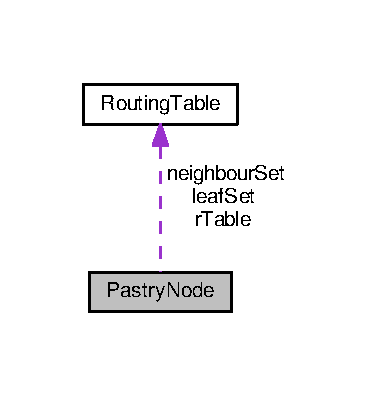
\includegraphics[width=178pt]{structPastryNode__coll__graph}
\end{center}
\end{figure}
\subsection*{Public Attributes}
\begin{DoxyCompactItemize}
\item 
char \hyperlink{structPastryNode_a2d2056d1f2b89b7369d1b96a38c6a5ae}{node\-I\-D} \mbox{[}9\mbox{]}
\item 
char \hyperlink{structPastryNode_a810f7ecb9b6479076a6ef533382b6fe1}{server\-\_\-ip\-\_\-port} \mbox{[}22\mbox{]}
\item 
struct \hyperlink{structRoutingTable}{Routing\-Table} \hyperlink{structPastryNode_a6092d47e197f9df34a0b29613cd2a053}{r\-Table} \mbox{[}8\mbox{]}\mbox{[}16\mbox{]}
\item 
struct \hyperlink{structRoutingTable}{Routing\-Table} \hyperlink{structPastryNode_aa529c7f78df5bb37013eeb96a2f4f83d}{leaf\-Set} \mbox{[}4\mbox{]}
\item 
struct \hyperlink{structRoutingTable}{Routing\-Table} \hyperlink{structPastryNode_a89eba401351ef59d5892a47416b7b874}{neighbour\-Set} \mbox{[}4\mbox{]}
\item 
map$<$ string, string $>$ \hyperlink{structPastryNode_ac6fc5a45aefb40f056954664d4820423}{my\-Map}
\end{DoxyCompactItemize}


\subsection{Member Data Documentation}
\hypertarget{structPastryNode_aa529c7f78df5bb37013eeb96a2f4f83d}{\index{Pastry\-Node@{Pastry\-Node}!leaf\-Set@{leaf\-Set}}
\index{leaf\-Set@{leaf\-Set}!PastryNode@{Pastry\-Node}}
\subsubsection[{leaf\-Set}]{\setlength{\rightskip}{0pt plus 5cm}struct {\bf Routing\-Table} Pastry\-Node\-::leaf\-Set\mbox{[}4\mbox{]}}}\label{structPastryNode_aa529c7f78df5bb37013eeb96a2f4f83d}
\hypertarget{structPastryNode_ac6fc5a45aefb40f056954664d4820423}{\index{Pastry\-Node@{Pastry\-Node}!my\-Map@{my\-Map}}
\index{my\-Map@{my\-Map}!PastryNode@{Pastry\-Node}}
\subsubsection[{my\-Map}]{\setlength{\rightskip}{0pt plus 5cm}map$<$string,string$>$ Pastry\-Node\-::my\-Map}}\label{structPastryNode_ac6fc5a45aefb40f056954664d4820423}
\hypertarget{structPastryNode_a89eba401351ef59d5892a47416b7b874}{\index{Pastry\-Node@{Pastry\-Node}!neighbour\-Set@{neighbour\-Set}}
\index{neighbour\-Set@{neighbour\-Set}!PastryNode@{Pastry\-Node}}
\subsubsection[{neighbour\-Set}]{\setlength{\rightskip}{0pt plus 5cm}struct {\bf Routing\-Table} Pastry\-Node\-::neighbour\-Set\mbox{[}4\mbox{]}}}\label{structPastryNode_a89eba401351ef59d5892a47416b7b874}
\hypertarget{structPastryNode_a2d2056d1f2b89b7369d1b96a38c6a5ae}{\index{Pastry\-Node@{Pastry\-Node}!node\-I\-D@{node\-I\-D}}
\index{node\-I\-D@{node\-I\-D}!PastryNode@{Pastry\-Node}}
\subsubsection[{node\-I\-D}]{\setlength{\rightskip}{0pt plus 5cm}char Pastry\-Node\-::node\-I\-D\mbox{[}9\mbox{]}}}\label{structPastryNode_a2d2056d1f2b89b7369d1b96a38c6a5ae}
\hypertarget{structPastryNode_a6092d47e197f9df34a0b29613cd2a053}{\index{Pastry\-Node@{Pastry\-Node}!r\-Table@{r\-Table}}
\index{r\-Table@{r\-Table}!PastryNode@{Pastry\-Node}}
\subsubsection[{r\-Table}]{\setlength{\rightskip}{0pt plus 5cm}struct {\bf Routing\-Table} Pastry\-Node\-::r\-Table\mbox{[}8\mbox{]}\mbox{[}16\mbox{]}}}\label{structPastryNode_a6092d47e197f9df34a0b29613cd2a053}
\hypertarget{structPastryNode_a810f7ecb9b6479076a6ef533382b6fe1}{\index{Pastry\-Node@{Pastry\-Node}!server\-\_\-ip\-\_\-port@{server\-\_\-ip\-\_\-port}}
\index{server\-\_\-ip\-\_\-port@{server\-\_\-ip\-\_\-port}!PastryNode@{Pastry\-Node}}
\subsubsection[{server\-\_\-ip\-\_\-port}]{\setlength{\rightskip}{0pt plus 5cm}char Pastry\-Node\-::server\-\_\-ip\-\_\-port\mbox{[}22\mbox{]}}}\label{structPastryNode_a810f7ecb9b6479076a6ef533382b6fe1}


The documentation for this struct was generated from the following file\-:\begin{DoxyCompactItemize}
\item 
\hyperlink{pastryfinal_8cpp}{pastryfinal.\-cpp}\end{DoxyCompactItemize}

\hypertarget{structRoutingTable}{\section{Routing\-Table Struct Reference}
\label{structRoutingTable}\index{Routing\-Table@{Routing\-Table}}
}
\subsection*{Public Attributes}
\begin{DoxyCompactItemize}
\item 
char \hyperlink{structRoutingTable_a68e60b82de7028edf994a6947b5419ae}{node\-Entry} \mbox{[}9\mbox{]}
\item 
char \hyperlink{structRoutingTable_a78bd90c64e38c527a16ed702ca9c2b00}{ip} \mbox{[}22\mbox{]}
\end{DoxyCompactItemize}


\subsection{Member Data Documentation}
\hypertarget{structRoutingTable_a78bd90c64e38c527a16ed702ca9c2b00}{\index{Routing\-Table@{Routing\-Table}!ip@{ip}}
\index{ip@{ip}!RoutingTable@{Routing\-Table}}
\subsubsection[{ip}]{\setlength{\rightskip}{0pt plus 5cm}char Routing\-Table\-::ip\mbox{[}22\mbox{]}}}\label{structRoutingTable_a78bd90c64e38c527a16ed702ca9c2b00}
\hypertarget{structRoutingTable_a68e60b82de7028edf994a6947b5419ae}{\index{Routing\-Table@{Routing\-Table}!node\-Entry@{node\-Entry}}
\index{node\-Entry@{node\-Entry}!RoutingTable@{Routing\-Table}}
\subsubsection[{node\-Entry}]{\setlength{\rightskip}{0pt plus 5cm}char Routing\-Table\-::node\-Entry\mbox{[}9\mbox{]}}}\label{structRoutingTable_a68e60b82de7028edf994a6947b5419ae}


The documentation for this struct was generated from the following file\-:\begin{DoxyCompactItemize}
\item 
\hyperlink{pastryfinal_8cpp}{pastryfinal.\-cpp}\end{DoxyCompactItemize}

\chapter{File Documentation}
\hypertarget{md5_8cpp}{\section{md5.\-cpp File Reference}
\label{md5_8cpp}\index{md5.\-cpp@{md5.\-cpp}}
}
{\ttfamily \#include \char`\"{}md5.\-h\char`\"{}}\\*
{\ttfamily \#include $<$cstdio$>$}\\*
Include dependency graph for md5.\-cpp\-:
\nopagebreak
\begin{figure}[H]
\begin{center}
\leavevmode
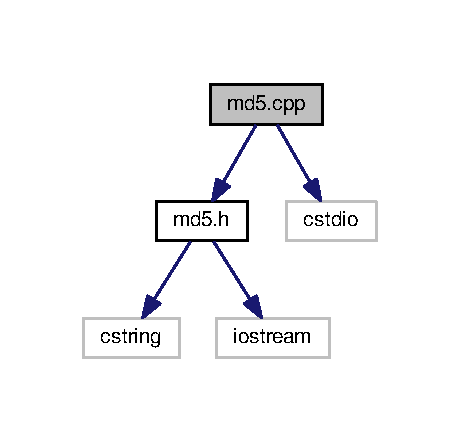
\includegraphics[width=220pt]{md5_8cpp__incl}
\end{center}
\end{figure}
\subsection*{Macros}
\begin{DoxyCompactItemize}
\item 
\#define \hyperlink{md5_8cpp_a51398c0e5541164ad4d6615880073305}{S11}~7
\item 
\#define \hyperlink{md5_8cpp_a1ec499cd0e54ecc28c2ac2afea5b038e}{S12}~12
\item 
\#define \hyperlink{md5_8cpp_aaeec90429105fb54d853dd4fc7027a54}{S13}~17
\item 
\#define \hyperlink{md5_8cpp_a78342b0ccde2ed12fdf19a113cc266cf}{S14}~22
\item 
\#define \hyperlink{md5_8cpp_ab6d5354f647a0e7592a1f051fc8377b2}{S21}~5
\item 
\#define \hyperlink{md5_8cpp_addad30455da936bc1879ee9c72b46d59}{S22}~9
\item 
\#define \hyperlink{md5_8cpp_a6321a8b29628936f76e9e78cf5bda95f}{S23}~14
\item 
\#define \hyperlink{md5_8cpp_a0c09eb77d30a0d5f9154914147b86c20}{S24}~20
\item 
\#define \hyperlink{md5_8cpp_aef26590f8a880ee6f4a158168defcd89}{S31}~4
\item 
\#define \hyperlink{md5_8cpp_a1d512424dd8a91e0a5bcc98563f33914}{S32}~11
\item 
\#define \hyperlink{md5_8cpp_a1c854214533f6220e859b0063196abb3}{S33}~16
\item 
\#define \hyperlink{md5_8cpp_af6472be1d535970afee8e5266a74aa07}{S34}~23
\item 
\#define \hyperlink{md5_8cpp_ab674ba129e588da55d1d494e1cf3c15e}{S41}~6
\item 
\#define \hyperlink{md5_8cpp_a268ef1a49114a94b931cc6b313e3cd1b}{S42}~10
\item 
\#define \hyperlink{md5_8cpp_a5aaa7121f39650d472746942ca68f959}{S43}~15
\item 
\#define \hyperlink{md5_8cpp_a6a3989af72b55d169bd73a66f8620aae}{S44}~21
\end{DoxyCompactItemize}
\subsection*{Functions}
\begin{DoxyCompactItemize}
\item 
std\-::ostream \& \hyperlink{md5_8cpp_a80cbf042ee22a0e557ac7938a6218e55}{operator$<$$<$} (std\-::ostream \&out, \hyperlink{classMD5}{M\-D5} \hyperlink{md5_8h_a92c6eed2e9b51298af559aff6792770b}{md5})
\item 
std\-::string \hyperlink{md5_8cpp_a92c6eed2e9b51298af559aff6792770b}{md5} (const std\-::string str)
\end{DoxyCompactItemize}


\subsection{Macro Definition Documentation}
\hypertarget{md5_8cpp_a51398c0e5541164ad4d6615880073305}{\index{md5.\-cpp@{md5.\-cpp}!S11@{S11}}
\index{S11@{S11}!md5.cpp@{md5.\-cpp}}
\subsubsection[{S11}]{\setlength{\rightskip}{0pt plus 5cm}\#define S11~7}}\label{md5_8cpp_a51398c0e5541164ad4d6615880073305}
\hypertarget{md5_8cpp_a1ec499cd0e54ecc28c2ac2afea5b038e}{\index{md5.\-cpp@{md5.\-cpp}!S12@{S12}}
\index{S12@{S12}!md5.cpp@{md5.\-cpp}}
\subsubsection[{S12}]{\setlength{\rightskip}{0pt plus 5cm}\#define S12~12}}\label{md5_8cpp_a1ec499cd0e54ecc28c2ac2afea5b038e}
\hypertarget{md5_8cpp_aaeec90429105fb54d853dd4fc7027a54}{\index{md5.\-cpp@{md5.\-cpp}!S13@{S13}}
\index{S13@{S13}!md5.cpp@{md5.\-cpp}}
\subsubsection[{S13}]{\setlength{\rightskip}{0pt plus 5cm}\#define S13~17}}\label{md5_8cpp_aaeec90429105fb54d853dd4fc7027a54}
\hypertarget{md5_8cpp_a78342b0ccde2ed12fdf19a113cc266cf}{\index{md5.\-cpp@{md5.\-cpp}!S14@{S14}}
\index{S14@{S14}!md5.cpp@{md5.\-cpp}}
\subsubsection[{S14}]{\setlength{\rightskip}{0pt plus 5cm}\#define S14~22}}\label{md5_8cpp_a78342b0ccde2ed12fdf19a113cc266cf}
\hypertarget{md5_8cpp_ab6d5354f647a0e7592a1f051fc8377b2}{\index{md5.\-cpp@{md5.\-cpp}!S21@{S21}}
\index{S21@{S21}!md5.cpp@{md5.\-cpp}}
\subsubsection[{S21}]{\setlength{\rightskip}{0pt plus 5cm}\#define S21~5}}\label{md5_8cpp_ab6d5354f647a0e7592a1f051fc8377b2}
\hypertarget{md5_8cpp_addad30455da936bc1879ee9c72b46d59}{\index{md5.\-cpp@{md5.\-cpp}!S22@{S22}}
\index{S22@{S22}!md5.cpp@{md5.\-cpp}}
\subsubsection[{S22}]{\setlength{\rightskip}{0pt plus 5cm}\#define S22~9}}\label{md5_8cpp_addad30455da936bc1879ee9c72b46d59}
\hypertarget{md5_8cpp_a6321a8b29628936f76e9e78cf5bda95f}{\index{md5.\-cpp@{md5.\-cpp}!S23@{S23}}
\index{S23@{S23}!md5.cpp@{md5.\-cpp}}
\subsubsection[{S23}]{\setlength{\rightskip}{0pt plus 5cm}\#define S23~14}}\label{md5_8cpp_a6321a8b29628936f76e9e78cf5bda95f}
\hypertarget{md5_8cpp_a0c09eb77d30a0d5f9154914147b86c20}{\index{md5.\-cpp@{md5.\-cpp}!S24@{S24}}
\index{S24@{S24}!md5.cpp@{md5.\-cpp}}
\subsubsection[{S24}]{\setlength{\rightskip}{0pt plus 5cm}\#define S24~20}}\label{md5_8cpp_a0c09eb77d30a0d5f9154914147b86c20}
\hypertarget{md5_8cpp_aef26590f8a880ee6f4a158168defcd89}{\index{md5.\-cpp@{md5.\-cpp}!S31@{S31}}
\index{S31@{S31}!md5.cpp@{md5.\-cpp}}
\subsubsection[{S31}]{\setlength{\rightskip}{0pt plus 5cm}\#define S31~4}}\label{md5_8cpp_aef26590f8a880ee6f4a158168defcd89}
\hypertarget{md5_8cpp_a1d512424dd8a91e0a5bcc98563f33914}{\index{md5.\-cpp@{md5.\-cpp}!S32@{S32}}
\index{S32@{S32}!md5.cpp@{md5.\-cpp}}
\subsubsection[{S32}]{\setlength{\rightskip}{0pt plus 5cm}\#define S32~11}}\label{md5_8cpp_a1d512424dd8a91e0a5bcc98563f33914}
\hypertarget{md5_8cpp_a1c854214533f6220e859b0063196abb3}{\index{md5.\-cpp@{md5.\-cpp}!S33@{S33}}
\index{S33@{S33}!md5.cpp@{md5.\-cpp}}
\subsubsection[{S33}]{\setlength{\rightskip}{0pt plus 5cm}\#define S33~16}}\label{md5_8cpp_a1c854214533f6220e859b0063196abb3}
\hypertarget{md5_8cpp_af6472be1d535970afee8e5266a74aa07}{\index{md5.\-cpp@{md5.\-cpp}!S34@{S34}}
\index{S34@{S34}!md5.cpp@{md5.\-cpp}}
\subsubsection[{S34}]{\setlength{\rightskip}{0pt plus 5cm}\#define S34~23}}\label{md5_8cpp_af6472be1d535970afee8e5266a74aa07}
\hypertarget{md5_8cpp_ab674ba129e588da55d1d494e1cf3c15e}{\index{md5.\-cpp@{md5.\-cpp}!S41@{S41}}
\index{S41@{S41}!md5.cpp@{md5.\-cpp}}
\subsubsection[{S41}]{\setlength{\rightskip}{0pt plus 5cm}\#define S41~6}}\label{md5_8cpp_ab674ba129e588da55d1d494e1cf3c15e}
\hypertarget{md5_8cpp_a268ef1a49114a94b931cc6b313e3cd1b}{\index{md5.\-cpp@{md5.\-cpp}!S42@{S42}}
\index{S42@{S42}!md5.cpp@{md5.\-cpp}}
\subsubsection[{S42}]{\setlength{\rightskip}{0pt plus 5cm}\#define S42~10}}\label{md5_8cpp_a268ef1a49114a94b931cc6b313e3cd1b}
\hypertarget{md5_8cpp_a5aaa7121f39650d472746942ca68f959}{\index{md5.\-cpp@{md5.\-cpp}!S43@{S43}}
\index{S43@{S43}!md5.cpp@{md5.\-cpp}}
\subsubsection[{S43}]{\setlength{\rightskip}{0pt plus 5cm}\#define S43~15}}\label{md5_8cpp_a5aaa7121f39650d472746942ca68f959}
\hypertarget{md5_8cpp_a6a3989af72b55d169bd73a66f8620aae}{\index{md5.\-cpp@{md5.\-cpp}!S44@{S44}}
\index{S44@{S44}!md5.cpp@{md5.\-cpp}}
\subsubsection[{S44}]{\setlength{\rightskip}{0pt plus 5cm}\#define S44~21}}\label{md5_8cpp_a6a3989af72b55d169bd73a66f8620aae}


\subsection{Function Documentation}
\hypertarget{md5_8cpp_a92c6eed2e9b51298af559aff6792770b}{\index{md5.\-cpp@{md5.\-cpp}!md5@{md5}}
\index{md5@{md5}!md5.cpp@{md5.\-cpp}}
\subsubsection[{md5}]{\setlength{\rightskip}{0pt plus 5cm}std\-::string md5 (
\begin{DoxyParamCaption}
\item[{const std\-::string}]{str}
\end{DoxyParamCaption}
)}}\label{md5_8cpp_a92c6eed2e9b51298af559aff6792770b}

\begin{DoxyCode}
326 \{
327     \hyperlink{classMD5}{MD5} \hyperlink{md5_8cpp_a92c6eed2e9b51298af559aff6792770b}{md5} = \hyperlink{classMD5}{MD5}(str);
328  
329     \textcolor{keywordflow}{return} md5.\hyperlink{classMD5_ad36c65acf87e397bf717bc3defbc0c7a}{hexdigest}();
330 \}\end{DoxyCode}
\hypertarget{md5_8cpp_a80cbf042ee22a0e557ac7938a6218e55}{\index{md5.\-cpp@{md5.\-cpp}!operator$<$$<$@{operator$<$$<$}}
\index{operator$<$$<$@{operator$<$$<$}!md5.cpp@{md5.\-cpp}}
\subsubsection[{operator$<$$<$}]{\setlength{\rightskip}{0pt plus 5cm}std\-::ostream\& operator$<$$<$ (
\begin{DoxyParamCaption}
\item[{std\-::ostream \&}]{out, }
\item[{{\bf M\-D5}}]{md5}
\end{DoxyParamCaption}
)}}\label{md5_8cpp_a80cbf042ee22a0e557ac7938a6218e55}

\begin{DoxyCode}
319 \{
320   \textcolor{keywordflow}{return} out << md5.\hyperlink{classMD5_ad36c65acf87e397bf717bc3defbc0c7a}{hexdigest}();
321 \}
\end{DoxyCode}

\hypertarget{md5_8h}{\section{md5.\-h File Reference}
\label{md5_8h}\index{md5.\-h@{md5.\-h}}
}
{\ttfamily \#include $<$cstring$>$}\\*
{\ttfamily \#include $<$iostream$>$}\\*
Include dependency graph for md5.\-h\-:
\nopagebreak
\begin{figure}[H]
\begin{center}
\leavevmode
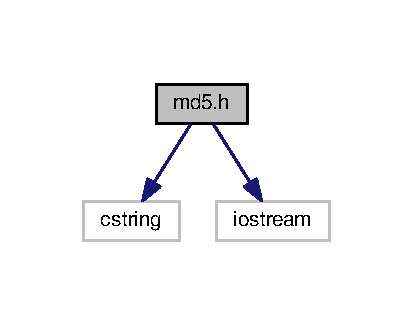
\includegraphics[width=198pt]{md5_8h__incl}
\end{center}
\end{figure}
This graph shows which files directly or indirectly include this file\-:
\nopagebreak
\begin{figure}[H]
\begin{center}
\leavevmode
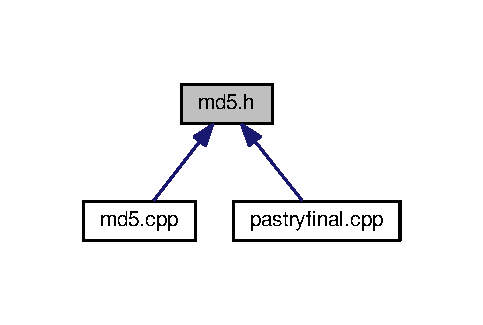
\includegraphics[width=232pt]{md5_8h__dep__incl}
\end{center}
\end{figure}
\subsection*{Classes}
\begin{DoxyCompactItemize}
\item 
class \hyperlink{classMD5}{M\-D5}
\end{DoxyCompactItemize}
\subsection*{Macros}
\begin{DoxyCompactItemize}
\item 
\#define \hyperlink{md5_8h_ac16c7a80c4d1e5f2c77e9b8c20e1ad64}{B\-Z\-F\-\_\-\-M\-D5\-\_\-\-H}
\item 
\#define \hyperlink{md5_8h_ac16c7a80c4d1e5f2c77e9b8c20e1ad64}{B\-Z\-F\-\_\-\-M\-D5\-\_\-\-H}
\end{DoxyCompactItemize}
\subsection*{Functions}
\begin{DoxyCompactItemize}
\item 
std\-::string \hyperlink{md5_8h_a92c6eed2e9b51298af559aff6792770b}{md5} (const std\-::string str)
\end{DoxyCompactItemize}


\subsection{Macro Definition Documentation}
\hypertarget{md5_8h_ac16c7a80c4d1e5f2c77e9b8c20e1ad64}{\index{md5.\-h@{md5.\-h}!B\-Z\-F\-\_\-\-M\-D5\-\_\-\-H@{B\-Z\-F\-\_\-\-M\-D5\-\_\-\-H}}
\index{B\-Z\-F\-\_\-\-M\-D5\-\_\-\-H@{B\-Z\-F\-\_\-\-M\-D5\-\_\-\-H}!md5.h@{md5.\-h}}
\subsubsection[{B\-Z\-F\-\_\-\-M\-D5\-\_\-\-H}]{\setlength{\rightskip}{0pt plus 5cm}\#define B\-Z\-F\-\_\-\-M\-D5\-\_\-\-H}}\label{md5_8h_ac16c7a80c4d1e5f2c77e9b8c20e1ad64}
\hypertarget{md5_8h_ac16c7a80c4d1e5f2c77e9b8c20e1ad64}{\index{md5.\-h@{md5.\-h}!B\-Z\-F\-\_\-\-M\-D5\-\_\-\-H@{B\-Z\-F\-\_\-\-M\-D5\-\_\-\-H}}
\index{B\-Z\-F\-\_\-\-M\-D5\-\_\-\-H@{B\-Z\-F\-\_\-\-M\-D5\-\_\-\-H}!md5.h@{md5.\-h}}
\subsubsection[{B\-Z\-F\-\_\-\-M\-D5\-\_\-\-H}]{\setlength{\rightskip}{0pt plus 5cm}\#define B\-Z\-F\-\_\-\-M\-D5\-\_\-\-H}}\label{md5_8h_ac16c7a80c4d1e5f2c77e9b8c20e1ad64}


\subsection{Function Documentation}
\hypertarget{md5_8h_a92c6eed2e9b51298af559aff6792770b}{\index{md5.\-h@{md5.\-h}!md5@{md5}}
\index{md5@{md5}!md5.h@{md5.\-h}}
\subsubsection[{md5}]{\setlength{\rightskip}{0pt plus 5cm}std\-::string md5 (
\begin{DoxyParamCaption}
\item[{const std\-::string}]{str}
\end{DoxyParamCaption}
)}}\label{md5_8h_a92c6eed2e9b51298af559aff6792770b}

\begin{DoxyCode}
326 \{
327     \hyperlink{classMD5}{MD5} \hyperlink{md5_8cpp_a92c6eed2e9b51298af559aff6792770b}{md5} = \hyperlink{classMD5}{MD5}(str);
328  
329     \textcolor{keywordflow}{return} md5.\hyperlink{classMD5_ad36c65acf87e397bf717bc3defbc0c7a}{hexdigest}();
330 \}\end{DoxyCode}

\hypertarget{pastryfinal_8cpp}{\section{pastryfinal.\-cpp File Reference}
\label{pastryfinal_8cpp}\index{pastryfinal.\-cpp@{pastryfinal.\-cpp}}
}
{\ttfamily \#include $<$iostream$>$}\\*
{\ttfamily \#include $<$sys/types.\-h$>$}\\*
{\ttfamily \#include $<$sys/socket.\-h$>$}\\*
{\ttfamily \#include $<$netinet/in.\-h$>$}\\*
{\ttfamily \#include $<$netdb.\-h$>$}\\*
{\ttfamily \#include $<$arpa/inet.\-h$>$}\\*
{\ttfamily \#include $<$ifaddrs.\-h$>$}\\*
{\ttfamily \#include $<$stdio.\-h$>$}\\*
{\ttfamily \#include $<$stdlib.\-h$>$}\\*
{\ttfamily \#include $<$unistd.\-h$>$}\\*
{\ttfamily \#include $<$errno.\-h$>$}\\*
{\ttfamily \#include $<$string.\-h$>$}\\*
{\ttfamily \#include $<$string$>$}\\*
{\ttfamily \#include $<$map$>$}\\*
{\ttfamily \#include $<$openssl/evp.\-h$>$}\\*
{\ttfamily \#include $<$math.\-h$>$}\\*
{\ttfamily \#include $<$pthread.\-h$>$}\\*
{\ttfamily \#include $<$zlib.\-h$>$}\\*
{\ttfamily \#include $<$vector$>$}\\*
{\ttfamily \#include $<$sstream$>$}\\*
{\ttfamily \#include $<$iomanip$>$}\\*
{\ttfamily \#include $<$utility$>$}\\*
{\ttfamily \#include \char`\"{}md5.\-h\char`\"{}}\\*
Include dependency graph for pastryfinal.\-cpp\-:
\nopagebreak
\begin{figure}[H]
\begin{center}
\leavevmode
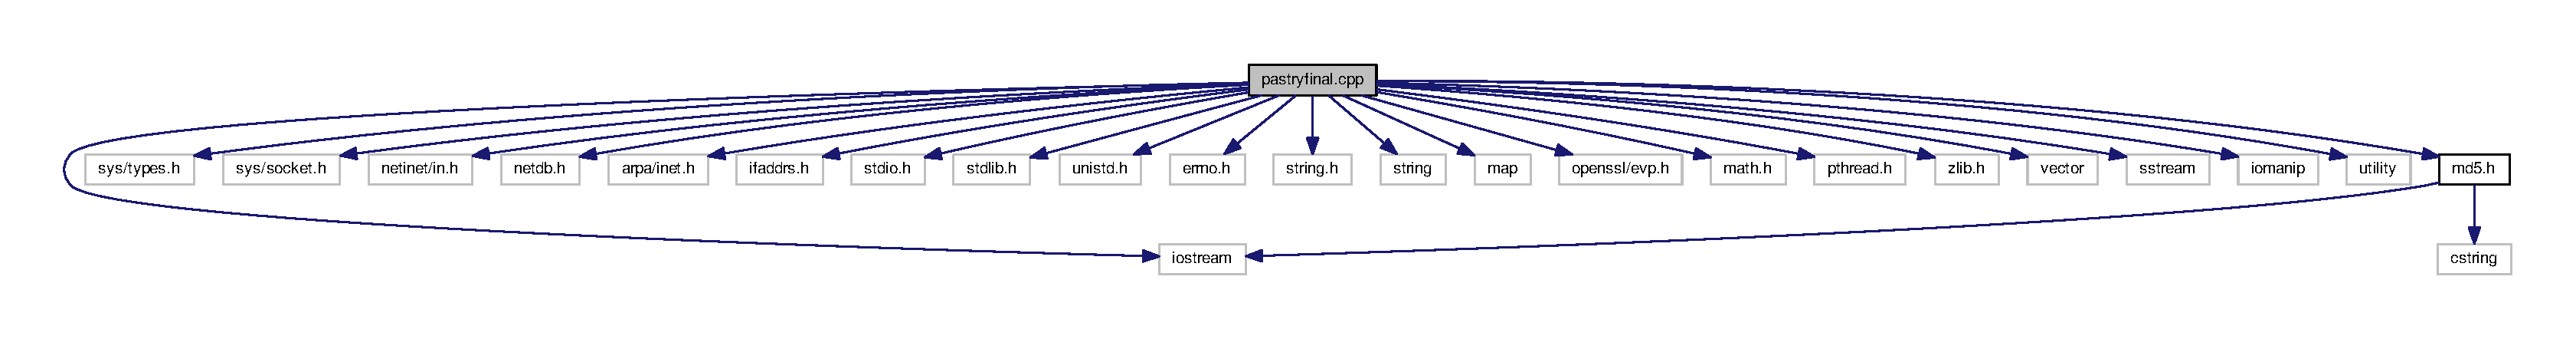
\includegraphics[width=350pt]{pastryfinal_8cpp__incl}
\end{center}
\end{figure}
\subsection*{Classes}
\begin{DoxyCompactItemize}
\item 
struct \hyperlink{structRoutingTable}{Routing\-Table}
\item 
struct \hyperlink{structPastryNode}{Pastry\-Node}
\end{DoxyCompactItemize}
\subsection*{Macros}
\begin{DoxyCompactItemize}
\item 
\#define \hyperlink{pastryfinal_8cpp_a89e0f81d51b75f05bc8f3b7cde0233d0}{D\-A\-T\-A\-\_\-\-S\-I\-Z\-E\-\_\-\-K\-I\-L\-O}~12000
\item 
\#define \hyperlink{pastryfinal_8cpp_a2b0b8b640f7863e341022226a4084ad9}{I\-P\-\_\-\-S\-I\-Z\-E}~40
\item 
\#define \hyperlink{pastryfinal_8cpp_abe3dabb3e10bf03a92a0d1c1672f62b6}{S\-E\-R\-V\-E\-R\-\_\-\-B\-U\-S\-Y}~'x'
\item 
\#define \hyperlink{pastryfinal_8cpp_a8de518a0f7ee14522952f707ce2dbbf1}{S\-A\-T\-\_\-\-M\-O\-D\-E}~\char`\"{}satm\char`\"{}
\item 
\#define \hyperlink{pastryfinal_8cpp_aa045b6864425ecb90f2c253e8440d21c}{N\-O\-R\-M\-A\-L\-\_\-\-M\-O\-D\-E}~\char`\"{}norm\char`\"{}
\end{DoxyCompactItemize}
\subsection*{Functions}
\begin{DoxyCompactItemize}
\item 
void \hyperlink{pastryfinal_8cpp_a468bd692c216e575d021f44568fc1157}{helper\-Put} (char $\ast$)
\item 
void \hyperlink{pastryfinal_8cpp_a6452aff3e646d22f67649cea090dbade}{store\-In\-Key\-Map} (char $\ast$)
\item 
void \hyperlink{pastryfinal_8cpp_ae1763fdff5462f8c3e6dd9847ad213a8}{print\-Dest\-Key\-Map} (char $\ast$)
\item 
void \hyperlink{pastryfinal_8cpp_a3e8373193ae1f11a9b04a7ae28d249b3}{helper\-Get} (char $\ast$)
\item 
void \hyperlink{pastryfinal_8cpp_a142e6a4218dba36486affd3276281242}{print\-Key\-Value} (char $\ast$)
\item 
void \hyperlink{pastryfinal_8cpp_a8ded397ed996b6269e734242eda2467a}{get\-Value\-For\-Key} (char $\ast$, char $\ast$)
\item 
int \hyperlink{pastryfinal_8cpp_a9c15e80b8820a8fd7e9e189c20fcaedd}{prefix} (char $\ast$, char $\ast$)
\item 
void \hyperlink{pastryfinal_8cpp_a22ed96355736095f167f22c16f2be7ae}{print\-My\-Keys} ()
\item 
void \hyperlink{pastryfinal_8cpp_ae521f52de7d40edb90b5b6c42caa61e0}{helper\-Dump} ()
\item 
void \hyperlink{pastryfinal_8cpp_a1c1fde8adc5a67d57281c25272a0b2b5}{helper\-Self} ()
\item 
bool \hyperlink{pastryfinal_8cpp_a92585621ba18a3ed294c6d13ee797655}{is\-Key\-Present\-In\-Map} (char $\ast$)
\item 
void \hyperlink{pastryfinal_8cpp_af53bffeda7bda17dda8ee69fd19b06e2}{update\-Recv\-Value} (char $\ast$)
\item 
long int \hyperlink{pastryfinal_8cpp_acc387a1e2442cd88fb4a313b29d64b1b}{absolute} (long int val)
\item 
char $\ast$ \hyperlink{pastryfinal_8cpp_a6267c19ae253842dbeeed10b3a846eb2}{substring} (char $\ast$string, int position, int length)
\item 
int \hyperlink{pastryfinal_8cpp_a3a587d9300fa6175e65ca3a41eab5279}{hex\-To\-Decimal} (char c)
\item 
char \hyperlink{pastryfinal_8cpp_ab9bfff8919fdf178d4c03431064fa2df}{decimal\-To\-Hex} (int i)
\item 
char $\ast$ \hyperlink{pastryfinal_8cpp_a1dd389d77cbb824b2aaf0d3b5fda5312}{decrement} (char $\ast$c, int i)
\item 
long int \hyperlink{pastryfinal_8cpp_a18e0867f46092f6c257671dae59f1b36}{hex\-String\-To\-Int} (char $\ast$str)
\item 
char $\ast$ \hyperlink{pastryfinal_8cpp_af26f3b71104fca10f7b8d6772c62b4bc}{calc\-\_\-hex\-\_\-diff} (char $\ast$n1, char $\ast$n2)
\item 
char $\ast$ \hyperlink{pastryfinal_8cpp_a2ad53a16e1556c8671a7b59625363f97}{calc\-\_\-hex\-\_\-sum} (char $\ast$n1, char $\ast$n2)
\item 
long int \hyperlink{pastryfinal_8cpp_a27351166f800aa7b19a73e7263982cc5}{calc\-\_\-min\-\_\-hex\-\_\-difference} (char $\ast$n1, char $\ast$n2)
\item 
int \hyperlink{pastryfinal_8cpp_a4c9699205efd1ee2e29abc56c0500f73}{index\-Of} (char $\ast$string, char of)
\item 
void \hyperlink{pastryfinal_8cpp_ab031a82c4539538a9102cae9c4a91458}{helper\-Help} ()
\item 
const char $\ast$ \hyperlink{pastryfinal_8cpp_a8fa2b8c55fe57bd42a07e3003e71358d}{hash\-Value} (const char $\ast$ip\-Port)
\item 
char \hyperlink{pastryfinal_8cpp_a6f0368b200fec3aecdb28f198c638c3b}{binary\-To\-Hex} (char $\ast$c1)
\item 
char $\ast$ \hyperlink{pastryfinal_8cpp_a57d6d12b551a24bebf60f7b2fe77fabc}{hex\-To\-Binary} (char c)
\item 
char $\ast$ \hyperlink{pastryfinal_8cpp_a5945104e9471526fc471409041b9e68f}{perform\-Xor} (char $\ast$c1, char $\ast$c2)
\item 
long int \hyperlink{pastryfinal_8cpp_a29e0a2388086c99b48ffc44ae6bd145d}{get\-Neighbour\-Distance} (char $\ast$Xnode\-I\-D)
\item 
void \hyperlink{pastryfinal_8cpp_a7dcf034cb1ffd8170cff3d49caca17b2}{print\-Current\-Leaf\-Set} ()
\item 
void \hyperlink{pastryfinal_8cpp_a9102e7eccfe3bf903e7405128d00742a}{print\-Current\-Neighbour\-Set} ()
\item 
void \hyperlink{pastryfinal_8cpp_a1b4bf23591332e697fd0b4ca029aaf8a}{print\-Current\-Routing\-Table} ()
\item 
bool \hyperlink{pastryfinal_8cpp_a6883fe4cc74905d454da109e053e43bd}{connect\-To\-Server} (int \&sock)
\item 
void \hyperlink{pastryfinal_8cpp_a7d0f00f54686b7ecfb1c73edca3ee4f4}{client} ()
\item 
void $\ast$ \hyperlink{pastryfinal_8cpp_a3679f5196b12605e3072f3086d5d4231}{reset} (void $\ast$arg)
\item 
void \hyperlink{pastryfinal_8cpp_a115e3d98ef69d6c97eccee42ec11d38d}{recv\-State\-Table} (char $\ast$str)
\item 
void \hyperlink{pastryfinal_8cpp_abb4efa658ce0ea4f573869e7594f8e77}{send\-State\-Table} (char $\ast$ipport)
\item 
void \hyperlink{pastryfinal_8cpp_aa35e17b04fd2ad03f7114555685e08aa}{insert\-X\-In\-Neighbour\-Set} (char $\ast$ip\-Port)
\item 
void \hyperlink{pastryfinal_8cpp_aec673b1eeef0340f3db2c31578edc022}{add\-Node\-To\-Pastry} (char $\ast$fcmd, char $\ast$ip\-Port)
\item 
void \hyperlink{pastryfinal_8cpp_a7d07f517b89cb9fb475f69dc144f2f6c}{send\-Keys} (char $\ast$ip\-Port)
\item 
void \hyperlink{pastryfinal_8cpp_acee6c6b14270974a7ee7d40c9c810291}{update\-X\-Entry} (char $\ast$ip\-Port)
\item 
void \hyperlink{pastryfinal_8cpp_a627622edff3c941da11bf793814eac08}{remove\-X\-Entry} (char $\ast$cmd)
\item 
void \hyperlink{pastryfinal_8cpp_ab3806dbbc38a26b3e07531ef8e9615a3}{send\-Requested\-Data} (char $\ast$cmd)
\item 
void \hyperlink{pastryfinal_8cpp_a7faa975c7da46b02b82b47a1309a30bf}{forward\-Command} ()
\item 
void \hyperlink{pastryfinal_8cpp_a2e72d907e4ac0cd9e674a5beb34d1a13}{send\-My\-Data\-Asked} (char $\ast$cmd)
\item 
void \hyperlink{pastryfinal_8cpp_a093f6efdf0d170922af9cd7ca96c9eda}{forward\-My\-Data\-Asked} (char $\ast$fcmd)
\item 
void $\ast$ \hyperlink{pastryfinal_8cpp_af012e0aa6674c56785bdad10e2b872d4}{execute\-Finger} (void $\ast$arg)
\item 
void \hyperlink{pastryfinal_8cpp_a2f2b76f5ca5f296be377aa8ae68b6a83}{helper\-Shut\-Down} ()
\item 
void \hyperlink{pastryfinal_8cpp_ab79321f704296b7049a6c7c09ab6af5c}{helper\-Finger} ()
\item 
void \hyperlink{pastryfinal_8cpp_a76a94da3dee6599446d1eeb06f577d96}{helper\-Dump\-All} ()
\item 
void \hyperlink{pastryfinal_8cpp_a8c2cedec69784642b4ee94ae1b725c69}{run\-Command} (char $\ast$cmd)
\item 
void \hyperlink{pastryfinal_8cpp_a9fae275b612d7d219589f514f5fd49fb}{update\-My\-Map} (char $\ast$cmd)
\item 
void \hyperlink{pastryfinal_8cpp_ad9f89a35bd039bd73e4c61eecaf348bd}{update\-State\-Tables} (char $\ast$cmd)
\item 
int \hyperlink{pastryfinal_8cpp_a44d8ac1af2e8754f6ababc8a13553e6e}{get\-Closet\-Leaf\-Index} ()
\item 
void \hyperlink{pastryfinal_8cpp_a99403f676431602751251f53b5b16263}{helper\-Quit} ()
\item 
void \hyperlink{pastryfinal_8cpp_a251e2ad37e848330e918ee00b2f59e47}{receive\-Route\-Table} (char $\ast$cmd)
\item 
void \hyperlink{pastryfinal_8cpp_a0fb882a6731b7db4c7f608f127653565}{receieve\-Leaf\-Set} (char $\ast$cmd)
\item 
void \hyperlink{pastryfinal_8cpp_a8ffd8c2d070313ba0271a55ba4992821}{recieve\-Neighbour\-Set} (char $\ast$cmd)
\item 
void \hyperlink{pastryfinal_8cpp_a50d190d1b7deaf7bc91d8e716f0ef150}{print\-Finger\-Data} (char $\ast$ip\-Port)
\item 
void \hyperlink{pastryfinal_8cpp_ad2389748d804e59b2968dfb1c3877de0}{print\-Dump\-Data} (char $\ast$Data)
\item 
void $\ast$ \hyperlink{pastryfinal_8cpp_a99bdc6ac85abe818a8047f8b5d20a2d7}{server} (void $\ast$arg)
\item 
char $\ast$ \hyperlink{pastryfinal_8cpp_ae8772c3a19ce9cf65fda2d5260f0e276}{get\-Self\-Ip\-Port} ()
\item 
void \hyperlink{pastryfinal_8cpp_a7962241d477be3e8f614619c77010003}{fill\-Node\-Entries} ()
\item 
void \hyperlink{pastryfinal_8cpp_aa83bad93098ea1d54dff28ae237473b2}{helper\-Create} ()
\item 
void \hyperlink{pastryfinal_8cpp_ac3252b0274a9243c5b9726ea4bb8fa5d}{helper\-Join} (char $\ast$cmd\-Data)
\item 
void \hyperlink{pastryfinal_8cpp_ace216b3a3671ae62b3214c3e95e4bcaa}{helperputsat} (char $\ast$str)
\item 
void \hyperlink{pastryfinal_8cpp_a82a31b53caab33e79a5a4cf265f01376}{helper\-Verify\-Sat} (char $\ast$str)
\item 
void \hyperlink{pastryfinal_8cpp_a58cb93359a143e99c2ab8d2388f1885b}{helper\-Get\-All\-Sat} (char $\ast$str)
\item 
void \hyperlink{pastryfinal_8cpp_a34e324a6daa93143460c37691d2c65f3}{help\-Helper\-Finger} ()
\item 
void \hyperlink{pastryfinal_8cpp_a6767908493d9b4495191746e1027fb33}{help\-Helper\-Dump\-All} ()
\item 
void \hyperlink{pastryfinal_8cpp_ac87c47da1891229705b5df82dca65015}{helper\-Print\-Route\-Table} (char $\ast$cmd)
\item 
void \hyperlink{pastryfinal_8cpp_a2e7bc4f207c102ab92ed2307b44bb9c1}{helper\-Print\-Leaf\-Set} (char $\ast$cmd)
\item 
void \hyperlink{pastryfinal_8cpp_aff992ddb41b041e2c5a1f31b69431d78}{helper\-Print\-Neighbour\-Set} (char $\ast$cmd)
\item 
void \hyperlink{pastryfinal_8cpp_a6991fb0afed08eeb21882d686c1a3114}{helper\-Print\-Dump} (char $\ast$cmd)
\item 
void \hyperlink{pastryfinal_8cpp_a4a1fdb1788f68507b7eedf25211ea301}{helper\-Route\-Table} (char $\ast$Data)
\item 
void \hyperlink{pastryfinal_8cpp_a22b5e9295406409e56a919dade9b0bb6}{helper\-Port} (char $\ast$cmd)
\item 
void \hyperlink{pastryfinal_8cpp_aad45f0999503b49219bcdfef99d14c09}{execute\-Command} ()
\item 
int \hyperlink{pastryfinal_8cpp_a0ddf1224851353fc92bfbff6f499fa97}{main} (int argc, char $\ast$argv\mbox{[}$\,$\mbox{]})
\end{DoxyCompactItemize}
\subsection*{Variables}
\begin{DoxyCompactItemize}
\item 
char \hyperlink{pastryfinal_8cpp_a5ca3a49008fc4cbde63d55a0f19aa17c}{ui\-\_\-data} \mbox{[}\hyperlink{pastryfinal_8cpp_a89e0f81d51b75f05bc8f3b7cde0233d0}{D\-A\-T\-A\-\_\-\-S\-I\-Z\-E\-\_\-\-K\-I\-L\-O}\mbox{]}
\item 
char \hyperlink{pastryfinal_8cpp_ac9675264bc1bfaf547e47f10073ecfb4}{server\-\_\-send\-\_\-data} \mbox{[}\hyperlink{pastryfinal_8cpp_a89e0f81d51b75f05bc8f3b7cde0233d0}{D\-A\-T\-A\-\_\-\-S\-I\-Z\-E\-\_\-\-K\-I\-L\-O}\mbox{]}
\item 
char \hyperlink{pastryfinal_8cpp_a69fb389cc58d682182528040876cead8}{server\-\_\-recv\-\_\-data} \mbox{[}\hyperlink{pastryfinal_8cpp_a89e0f81d51b75f05bc8f3b7cde0233d0}{D\-A\-T\-A\-\_\-\-S\-I\-Z\-E\-\_\-\-K\-I\-L\-O}\mbox{]}
\item 
char \hyperlink{pastryfinal_8cpp_a0c095ae203cce061e0e8c3ae9025ab94}{client\-\_\-send\-\_\-data} \mbox{[}\hyperlink{pastryfinal_8cpp_a89e0f81d51b75f05bc8f3b7cde0233d0}{D\-A\-T\-A\-\_\-\-S\-I\-Z\-E\-\_\-\-K\-I\-L\-O}\mbox{]}
\item 
char \hyperlink{pastryfinal_8cpp_a538d93f9ad243e6a20d0468a37094c39}{client\-\_\-recv\-\_\-data} \mbox{[}\hyperlink{pastryfinal_8cpp_a89e0f81d51b75f05bc8f3b7cde0233d0}{D\-A\-T\-A\-\_\-\-S\-I\-Z\-E\-\_\-\-K\-I\-L\-O}\mbox{]}
\item 
char \hyperlink{pastryfinal_8cpp_a062486df77f175d79bd505da7626bba5}{ff\-\_\-client\-\_\-send\-\_\-data} \mbox{[}\hyperlink{pastryfinal_8cpp_a89e0f81d51b75f05bc8f3b7cde0233d0}{D\-A\-T\-A\-\_\-\-S\-I\-Z\-E\-\_\-\-K\-I\-L\-O}\mbox{]}
\item 
char \hyperlink{pastryfinal_8cpp_ab925fbb6c6e14c2aac0afcf3a5f409e3}{ff\-\_\-client\-\_\-recv\-\_\-data} \mbox{[}\hyperlink{pastryfinal_8cpp_a89e0f81d51b75f05bc8f3b7cde0233d0}{D\-A\-T\-A\-\_\-\-S\-I\-Z\-E\-\_\-\-K\-I\-L\-O}\mbox{]}
\item 
char \hyperlink{pastryfinal_8cpp_acece90d87b107a3bddb23511a4ed7fa4}{dd\-\_\-client\-\_\-send\-\_\-data} \mbox{[}\hyperlink{pastryfinal_8cpp_a89e0f81d51b75f05bc8f3b7cde0233d0}{D\-A\-T\-A\-\_\-\-S\-I\-Z\-E\-\_\-\-K\-I\-L\-O}\mbox{]}
\item 
char \hyperlink{pastryfinal_8cpp_a08cf3708785702a364c84f794ff7d7c1}{dd\-\_\-client\-\_\-recv\-\_\-data} \mbox{[}\hyperlink{pastryfinal_8cpp_a89e0f81d51b75f05bc8f3b7cde0233d0}{D\-A\-T\-A\-\_\-\-S\-I\-Z\-E\-\_\-\-K\-I\-L\-O}\mbox{]}
\item 
unsigned int \hyperlink{pastryfinal_8cpp_a3ebc706f0e54e0b203467570244b0ca3}{server\-\_\-port} = 0
\item 
int \hyperlink{pastryfinal_8cpp_adefe76971a34b75ad8f6b1363959e558}{server\-Sock}
\item 
bool \hyperlink{pastryfinal_8cpp_ad0749475175c0944e0379c12910a8b48}{is\-Created} = false
\item 
bool \hyperlink{pastryfinal_8cpp_a57f6de21dc67db4f40e381eb356db18d}{has\-Joined} = false
\item 
int \hyperlink{pastryfinal_8cpp_a79d9a1941d35eea97ea57ea98d6ac2ae}{retry\-\_\-count} = 5
\item 
int \hyperlink{pastryfinal_8cpp_a1beeff7e5f8d525c010c132183d8fdc0}{nop} = 3
\item 
unsigned int \hyperlink{pastryfinal_8cpp_a938bdc6ae46c346147b6d4f67ad1e704}{port} = 0
\item 
char $\ast$ \hyperlink{pastryfinal_8cpp_a94ec905a3fc10207acdd27707182f337}{s\-Port}
\item 
char $\ast$ \hyperlink{pastryfinal_8cpp_af3e6c6fd14559b2176c2ba6848bffe2a}{dest\-Port}
\item 
char \hyperlink{pastryfinal_8cpp_a965c131de25d30c7aaf9269ad4b03222}{first\-\_\-ip\-Port} \mbox{[}22\mbox{]}
\item 
const char $\ast$ \hyperlink{pastryfinal_8cpp_a162736b74a8b74ce0c347b17b597928f}{dest\-I\-P}
\item 
char \hyperlink{pastryfinal_8cpp_a4318aba8f1dbec9f9819784eb1d7b0d8}{recv\-\_\-value} \mbox{[}4\mbox{]}
\item 
char \hyperlink{pastryfinal_8cpp_aa7cc75a672640c573291d1a53ab63d71}{mode} \mbox{[}4\mbox{]}
\item 
char \hyperlink{pastryfinal_8cpp_a6505a024ecdb42cacc1baa97656161c1}{key\-\_\-value} \mbox{[}20\mbox{]}
\item 
char \hyperlink{pastryfinal_8cpp_a0c42167b6bee371acf2f3c52c01df552}{cor\-\_\-get\-\_\-value} \mbox{[}6\mbox{]}
\item 
int \hyperlink{pastryfinal_8cpp_a72e27dee31b1c4c6a504fbed29542d97}{last} =0
\item 
int \hyperlink{pastryfinal_8cpp_ac8261e7cbff4aff66263175e1ca2b2a9}{f\-R} =0
\item 
int \hyperlink{pastryfinal_8cpp_ad3c05a32c566761a7a4c7759ed3d5986}{recvd\-\_\-last} =0
\item 
char \hyperlink{pastryfinal_8cpp_a4211c8ae3d8024a31c0414ee15aceafc}{cmd\-In\-Exec} \mbox{[}10\mbox{]}
\item 
bool \hyperlink{pastryfinal_8cpp_ac5746c41564997a51f0fb9cab1ef927c}{shut\-Flag} =false
\item 
bool \hyperlink{pastryfinal_8cpp_af2d5a9c696d1d55b6b8194ce63eb45ca}{is\-Sending} =false
\item 
bool \hyperlink{pastryfinal_8cpp_a8feac6df73e1c19e619f21887b094124}{dmp\-Flag} =false
\item 
bool \hyperlink{pastryfinal_8cpp_afbaf51ae23b8fefd3921e375b4b417ef}{getsat} =false
\item 
struct \hyperlink{structPastryNode}{Pastry\-Node} Node \hyperlink{pastryfinal_8cpp_a7d0867968b662a0ed1dc24d0633cf107}{recvd}
\end{DoxyCompactItemize}


\subsection{Macro Definition Documentation}
\hypertarget{pastryfinal_8cpp_a89e0f81d51b75f05bc8f3b7cde0233d0}{\index{pastryfinal.\-cpp@{pastryfinal.\-cpp}!D\-A\-T\-A\-\_\-\-S\-I\-Z\-E\-\_\-\-K\-I\-L\-O@{D\-A\-T\-A\-\_\-\-S\-I\-Z\-E\-\_\-\-K\-I\-L\-O}}
\index{D\-A\-T\-A\-\_\-\-S\-I\-Z\-E\-\_\-\-K\-I\-L\-O@{D\-A\-T\-A\-\_\-\-S\-I\-Z\-E\-\_\-\-K\-I\-L\-O}!pastryfinal.cpp@{pastryfinal.\-cpp}}
\subsubsection[{D\-A\-T\-A\-\_\-\-S\-I\-Z\-E\-\_\-\-K\-I\-L\-O}]{\setlength{\rightskip}{0pt plus 5cm}\#define D\-A\-T\-A\-\_\-\-S\-I\-Z\-E\-\_\-\-K\-I\-L\-O~12000}}\label{pastryfinal_8cpp_a89e0f81d51b75f05bc8f3b7cde0233d0}
\hypertarget{pastryfinal_8cpp_a2b0b8b640f7863e341022226a4084ad9}{\index{pastryfinal.\-cpp@{pastryfinal.\-cpp}!I\-P\-\_\-\-S\-I\-Z\-E@{I\-P\-\_\-\-S\-I\-Z\-E}}
\index{I\-P\-\_\-\-S\-I\-Z\-E@{I\-P\-\_\-\-S\-I\-Z\-E}!pastryfinal.cpp@{pastryfinal.\-cpp}}
\subsubsection[{I\-P\-\_\-\-S\-I\-Z\-E}]{\setlength{\rightskip}{0pt plus 5cm}\#define I\-P\-\_\-\-S\-I\-Z\-E~40}}\label{pastryfinal_8cpp_a2b0b8b640f7863e341022226a4084ad9}
\hypertarget{pastryfinal_8cpp_aa045b6864425ecb90f2c253e8440d21c}{\index{pastryfinal.\-cpp@{pastryfinal.\-cpp}!N\-O\-R\-M\-A\-L\-\_\-\-M\-O\-D\-E@{N\-O\-R\-M\-A\-L\-\_\-\-M\-O\-D\-E}}
\index{N\-O\-R\-M\-A\-L\-\_\-\-M\-O\-D\-E@{N\-O\-R\-M\-A\-L\-\_\-\-M\-O\-D\-E}!pastryfinal.cpp@{pastryfinal.\-cpp}}
\subsubsection[{N\-O\-R\-M\-A\-L\-\_\-\-M\-O\-D\-E}]{\setlength{\rightskip}{0pt plus 5cm}\#define N\-O\-R\-M\-A\-L\-\_\-\-M\-O\-D\-E~\char`\"{}norm\char`\"{}}}\label{pastryfinal_8cpp_aa045b6864425ecb90f2c253e8440d21c}
\hypertarget{pastryfinal_8cpp_a8de518a0f7ee14522952f707ce2dbbf1}{\index{pastryfinal.\-cpp@{pastryfinal.\-cpp}!S\-A\-T\-\_\-\-M\-O\-D\-E@{S\-A\-T\-\_\-\-M\-O\-D\-E}}
\index{S\-A\-T\-\_\-\-M\-O\-D\-E@{S\-A\-T\-\_\-\-M\-O\-D\-E}!pastryfinal.cpp@{pastryfinal.\-cpp}}
\subsubsection[{S\-A\-T\-\_\-\-M\-O\-D\-E}]{\setlength{\rightskip}{0pt plus 5cm}\#define S\-A\-T\-\_\-\-M\-O\-D\-E~\char`\"{}satm\char`\"{}}}\label{pastryfinal_8cpp_a8de518a0f7ee14522952f707ce2dbbf1}
\hypertarget{pastryfinal_8cpp_abe3dabb3e10bf03a92a0d1c1672f62b6}{\index{pastryfinal.\-cpp@{pastryfinal.\-cpp}!S\-E\-R\-V\-E\-R\-\_\-\-B\-U\-S\-Y@{S\-E\-R\-V\-E\-R\-\_\-\-B\-U\-S\-Y}}
\index{S\-E\-R\-V\-E\-R\-\_\-\-B\-U\-S\-Y@{S\-E\-R\-V\-E\-R\-\_\-\-B\-U\-S\-Y}!pastryfinal.cpp@{pastryfinal.\-cpp}}
\subsubsection[{S\-E\-R\-V\-E\-R\-\_\-\-B\-U\-S\-Y}]{\setlength{\rightskip}{0pt plus 5cm}\#define S\-E\-R\-V\-E\-R\-\_\-\-B\-U\-S\-Y~'x'}}\label{pastryfinal_8cpp_abe3dabb3e10bf03a92a0d1c1672f62b6}


\subsection{Function Documentation}
\hypertarget{pastryfinal_8cpp_acc387a1e2442cd88fb4a313b29d64b1b}{\index{pastryfinal.\-cpp@{pastryfinal.\-cpp}!absolute@{absolute}}
\index{absolute@{absolute}!pastryfinal.cpp@{pastryfinal.\-cpp}}
\subsubsection[{absolute}]{\setlength{\rightskip}{0pt plus 5cm}long int absolute (
\begin{DoxyParamCaption}
\item[{long int}]{val}
\end{DoxyParamCaption}
)}}\label{pastryfinal_8cpp_acc387a1e2442cd88fb4a313b29d64b1b}

\begin{DoxyCode}
102 \{
103     \textcolor{keywordflow}{if}(val<0)
104         \textcolor{keywordflow}{return} (val*(-1));
105     \textcolor{keywordflow}{else} 
106         \textcolor{keywordflow}{return} val;
107 \}
\end{DoxyCode}
\hypertarget{pastryfinal_8cpp_aec673b1eeef0340f3db2c31578edc022}{\index{pastryfinal.\-cpp@{pastryfinal.\-cpp}!add\-Node\-To\-Pastry@{add\-Node\-To\-Pastry}}
\index{add\-Node\-To\-Pastry@{add\-Node\-To\-Pastry}!pastryfinal.cpp@{pastryfinal.\-cpp}}
\subsubsection[{add\-Node\-To\-Pastry}]{\setlength{\rightskip}{0pt plus 5cm}void add\-Node\-To\-Pastry (
\begin{DoxyParamCaption}
\item[{char $\ast$}]{fcmd, }
\item[{char $\ast$}]{ip\-Port}
\end{DoxyParamCaption}
)}}\label{pastryfinal_8cpp_aec673b1eeef0340f3db2c31578edc022}

\begin{DoxyCode}
683 \{
684     \textcolor{keywordtype}{int} i,k;
685     \textcolor{keywordtype}{char} nextNodeId[9];
686     \textcolor{keywordtype}{char} dipPort[22];     \textcolor{comment}{//1st}
687     \textcolor{keywordtype}{char} XnodeID[9];
688     strcpy(XnodeID,\hyperlink{pastryfinal_8cpp_a8fa2b8c55fe57bd42a07e3003e71358d}{hashValue}(ipPort));
689     
690     \textcolor{keywordflow}{for}(i=0;i<8;i++)
691         \textcolor{keywordflow}{if}(XnodeID[i]!=Node.nodeID[i])
692             \textcolor{keywordflow}{break};
693 
694     \textcolor{keywordtype}{int} j=\hyperlink{pastryfinal_8cpp_a3a587d9300fa6175e65ca3a41eab5279}{hexToDecimal}(XnodeID[i]);
695 
696     \textcolor{keywordflow}{if}(Node.rTable[i][j].nodeEntry[0]!=\textcolor{charliteral}{'\(\backslash\)0'})
697     \{   
698         strcpy(nextNodeId, Node.rTable[i][j].nodeEntry);
699         strcpy(dipPort,Node.rTable[i][j].ip);
700     \}   
701     \textcolor{keywordflow}{else}    
702         \hyperlink{pastryfinal_8cpp_a72e27dee31b1c4c6a504fbed29542d97}{last} = 1;
703 
704     \hyperlink{pastryfinal_8cpp_abb4efa658ce0ea4f573869e7594f8e77}{sendStateTable}(ipPort);   
705 
706     \textcolor{keywordflow}{if}(\hyperlink{pastryfinal_8cpp_a72e27dee31b1c4c6a504fbed29542d97}{last}==0)
707     \{   
708     strcpy(\hyperlink{pastryfinal_8cpp_a0c095ae203cce061e0e8c3ae9025ab94}{client\_send\_data},\textcolor{stringliteral}{"cmd "});    
709     \hyperlink{pastryfinal_8cpp_a162736b74a8b74ce0c347b17b597928f}{destIP}=\hyperlink{pastryfinal_8cpp_a6267c19ae253842dbeeed10b3a846eb2}{substring}(dipPort,0,\hyperlink{pastryfinal_8cpp_a4c9699205efd1ee2e29abc56c0500f73}{indexOf}(dipPort,\textcolor{charliteral}{':'}));
710     \hyperlink{pastryfinal_8cpp_af3e6c6fd14559b2176c2ba6848bffe2a}{destPort}=\hyperlink{pastryfinal_8cpp_a6267c19ae253842dbeeed10b3a846eb2}{substring}(dipPort,\hyperlink{pastryfinal_8cpp_a4c9699205efd1ee2e29abc56c0500f73}{indexOf}(dipPort,\textcolor{charliteral}{':'})+1, strlen(dipPort)-
      \hyperlink{pastryfinal_8cpp_a4c9699205efd1ee2e29abc56c0500f73}{indexOf}(dipPort,\textcolor{charliteral}{':'})-1);
711     strcat(\hyperlink{pastryfinal_8cpp_a0c095ae203cce061e0e8c3ae9025ab94}{client\_send\_data},fcmd);
712     \hyperlink{pastryfinal_8cpp_a7d0f00f54686b7ecfb1c73edca3ee4f4}{client}();
713     \}
714 
715     \hyperlink{pastryfinal_8cpp_a72e27dee31b1c4c6a504fbed29542d97}{last}=0;
716 
717 \}
\end{DoxyCode}
\hypertarget{pastryfinal_8cpp_a6f0368b200fec3aecdb28f198c638c3b}{\index{pastryfinal.\-cpp@{pastryfinal.\-cpp}!binary\-To\-Hex@{binary\-To\-Hex}}
\index{binary\-To\-Hex@{binary\-To\-Hex}!pastryfinal.cpp@{pastryfinal.\-cpp}}
\subsubsection[{binary\-To\-Hex}]{\setlength{\rightskip}{0pt plus 5cm}char binary\-To\-Hex (
\begin{DoxyParamCaption}
\item[{char $\ast$}]{c1}
\end{DoxyParamCaption}
)}}\label{pastryfinal_8cpp_a6f0368b200fec3aecdb28f198c638c3b}

\begin{DoxyCode}
351 \{
352     \textcolor{keywordtype}{int} sum=0;
353     \textcolor{keywordflow}{for}(\textcolor{keywordtype}{int} i=0;i<4;i++)
354         sum+= ((\textcolor{keywordtype}{int})c1[i]-48)*((int)(pow(2,3-i)));
355 
356     \textcolor{keywordflow}{return} \hyperlink{pastryfinal_8cpp_ab9bfff8919fdf178d4c03431064fa2df}{decimalToHex}(sum);
357 \}
\end{DoxyCode}
\hypertarget{pastryfinal_8cpp_af26f3b71104fca10f7b8d6772c62b4bc}{\index{pastryfinal.\-cpp@{pastryfinal.\-cpp}!calc\-\_\-hex\-\_\-diff@{calc\-\_\-hex\-\_\-diff}}
\index{calc\-\_\-hex\-\_\-diff@{calc\-\_\-hex\-\_\-diff}!pastryfinal.cpp@{pastryfinal.\-cpp}}
\subsubsection[{calc\-\_\-hex\-\_\-diff}]{\setlength{\rightskip}{0pt plus 5cm}char$\ast$ calc\-\_\-hex\-\_\-diff (
\begin{DoxyParamCaption}
\item[{char $\ast$}]{n1, }
\item[{char $\ast$}]{n2}
\end{DoxyParamCaption}
)}}\label{pastryfinal_8cpp_af26f3b71104fca10f7b8d6772c62b4bc}

\begin{DoxyCode}
175 \{
176     \textcolor{keywordtype}{char} c1[9],c2[9],temp[9];
177     \textcolor{keywordtype}{char} *res;
178     res=(\textcolor{keywordtype}{char}*) malloc(9*\textcolor{keyword}{sizeof}(\textcolor{keywordtype}{char}));
179     strcpy(c1,n1);
180     strcpy(c2,n2);
181     \textcolor{keywordflow}{if}(strcmp(c1,c2)<0)
182     \{
183         strcpy(temp,c1);
184         strcpy(c1,c2);
185         strcpy(c2,temp);
186     \}   
187 
188     \textcolor{keywordflow}{for}(\textcolor{keywordtype}{int} i=7;i>=0;i--)
189     \{
190         \textcolor{keywordflow}{if}(c1[i]>c2[i])
191             res[i]=\hyperlink{pastryfinal_8cpp_ab9bfff8919fdf178d4c03431064fa2df}{decimalToHex}(\hyperlink{pastryfinal_8cpp_a3a587d9300fa6175e65ca3a41eab5279}{hexToDecimal}(c1[i])-
      \hyperlink{pastryfinal_8cpp_a3a587d9300fa6175e65ca3a41eab5279}{hexToDecimal}(c2[i]));
192         \textcolor{keywordflow}{else} \textcolor{keywordflow}{if}(c1[i]<c2[i])
193         \{
194             res[i]=\hyperlink{pastryfinal_8cpp_ab9bfff8919fdf178d4c03431064fa2df}{decimalToHex}(16+\hyperlink{pastryfinal_8cpp_a3a587d9300fa6175e65ca3a41eab5279}{hexToDecimal}(c1[i])-
      \hyperlink{pastryfinal_8cpp_a3a587d9300fa6175e65ca3a41eab5279}{hexToDecimal}(c2[i]));
195             strcpy(c1,\hyperlink{pastryfinal_8cpp_a1dd389d77cbb824b2aaf0d3b5fda5312}{decrement}(c1,i-1));
196         \}
197         \textcolor{keywordflow}{else}
198             res[i]=\textcolor{charliteral}{'0'}; 
199     \}   
200     res[8]=\textcolor{charliteral}{'\(\backslash\)0'};
201     \textcolor{keywordflow}{return} res;
202 \}
\end{DoxyCode}
\hypertarget{pastryfinal_8cpp_a2ad53a16e1556c8671a7b59625363f97}{\index{pastryfinal.\-cpp@{pastryfinal.\-cpp}!calc\-\_\-hex\-\_\-sum@{calc\-\_\-hex\-\_\-sum}}
\index{calc\-\_\-hex\-\_\-sum@{calc\-\_\-hex\-\_\-sum}!pastryfinal.cpp@{pastryfinal.\-cpp}}
\subsubsection[{calc\-\_\-hex\-\_\-sum}]{\setlength{\rightskip}{0pt plus 5cm}char$\ast$ calc\-\_\-hex\-\_\-sum (
\begin{DoxyParamCaption}
\item[{char $\ast$}]{n1, }
\item[{char $\ast$}]{n2}
\end{DoxyParamCaption}
)}}\label{pastryfinal_8cpp_a2ad53a16e1556c8671a7b59625363f97}

\begin{DoxyCode}
205 \{
206     \textcolor{keywordtype}{char}* res=(\textcolor{keywordtype}{char}*)malloc(9);
207     res[8]=\textcolor{charliteral}{'\(\backslash\)0'};
208     \textcolor{keywordtype}{long} \textcolor{keywordtype}{int} i = \hyperlink{pastryfinal_8cpp_a18e0867f46092f6c257671dae59f1b36}{hexStringToInt}(n1);
209     \textcolor{keywordtype}{long} \textcolor{keywordtype}{int} j = \hyperlink{pastryfinal_8cpp_a18e0867f46092f6c257671dae59f1b36}{hexStringToInt}(n2);
210     \textcolor{keywordtype}{long} \textcolor{keywordtype}{int} sum = i+j;
211 
212     \textcolor{keywordflow}{for}(\textcolor{keywordtype}{int} k=7;k>=0;k--)
213     \{
214         res[k]= \hyperlink{pastryfinal_8cpp_ab9bfff8919fdf178d4c03431064fa2df}{decimalToHex}(sum%16);
215         sum=sum/16;
216     \}
217 
218     \textcolor{keywordflow}{return} res; 
219 \}
\end{DoxyCode}
\hypertarget{pastryfinal_8cpp_a27351166f800aa7b19a73e7263982cc5}{\index{pastryfinal.\-cpp@{pastryfinal.\-cpp}!calc\-\_\-min\-\_\-hex\-\_\-difference@{calc\-\_\-min\-\_\-hex\-\_\-difference}}
\index{calc\-\_\-min\-\_\-hex\-\_\-difference@{calc\-\_\-min\-\_\-hex\-\_\-difference}!pastryfinal.cpp@{pastryfinal.\-cpp}}
\subsubsection[{calc\-\_\-min\-\_\-hex\-\_\-difference}]{\setlength{\rightskip}{0pt plus 5cm}long int calc\-\_\-min\-\_\-hex\-\_\-difference (
\begin{DoxyParamCaption}
\item[{char $\ast$}]{n1, }
\item[{char $\ast$}]{n2}
\end{DoxyParamCaption}
)}}\label{pastryfinal_8cpp_a27351166f800aa7b19a73e7263982cc5}

\begin{DoxyCode}
222 \{
223     \textcolor{keywordtype}{char} c1[9]=\textcolor{stringliteral}{"ffffffff"};
224     c1[8]=\textcolor{charliteral}{'\(\backslash\)0'};
225     \textcolor{keywordtype}{char}* temp;
226     \textcolor{keywordflow}{if}(n1[0]<n2[0])
227     \{
228         temp=n1;
229         n1=n2;
230         n2=temp;
231     \}   
232 
233     \textcolor{keywordtype}{char}* d1 = \hyperlink{pastryfinal_8cpp_af26f3b71104fca10f7b8d6772c62b4bc}{calc\_hex\_diff}(n1,n2);
234     \textcolor{keywordtype}{char}* d21 = \hyperlink{pastryfinal_8cpp_af26f3b71104fca10f7b8d6772c62b4bc}{calc\_hex\_diff}(c1,n1);
235     \textcolor{keywordtype}{char}* d2 = \hyperlink{pastryfinal_8cpp_a2ad53a16e1556c8671a7b59625363f97}{calc\_hex\_sum}(d21,n2);
236 
237     \textcolor{keywordflow}{if}(strcmp(d1,d2)<=0)
238         \textcolor{keywordflow}{return} \hyperlink{pastryfinal_8cpp_a18e0867f46092f6c257671dae59f1b36}{hexStringToInt}(d1);
239     \textcolor{keywordflow}{else}
240         \textcolor{keywordflow}{return} \hyperlink{pastryfinal_8cpp_a18e0867f46092f6c257671dae59f1b36}{hexStringToInt}(d2);
241 
242 \}
\end{DoxyCode}
\hypertarget{pastryfinal_8cpp_a7d0f00f54686b7ecfb1c73edca3ee4f4}{\index{pastryfinal.\-cpp@{pastryfinal.\-cpp}!client@{client}}
\index{client@{client}!pastryfinal.cpp@{pastryfinal.\-cpp}}
\subsubsection[{client}]{\setlength{\rightskip}{0pt plus 5cm}void client (
\begin{DoxyParamCaption}
{}
\end{DoxyParamCaption}
)}}\label{pastryfinal_8cpp_a7d0f00f54686b7ecfb1c73edca3ee4f4}

\begin{DoxyCode}
500 \{
501     \textcolor{keywordtype}{int} sock,bytes\_received;
502 
503     \textcolor{keywordflow}{if}(!\hyperlink{pastryfinal_8cpp_a6883fe4cc74905d454da109e053e43bd}{connectToServer}(sock))
504     \{
505         \textcolor{keywordflow}{if}(strcmp(\hyperlink{pastryfinal_8cpp_a4211c8ae3d8024a31c0414ee15aceafc}{cmdInExec},\textcolor{stringliteral}{"shutdown"})==0)
506             \textcolor{keywordflow}{return};
507         \hyperlink{pastryfinal_8cpp_a538d93f9ad243e6a20d0468a37094c39}{client\_recv\_data}[0] = \hyperlink{pastryfinal_8cpp_abe3dabb3e10bf03a92a0d1c1672f62b6}{SERVER\_BUSY};
508         cout<<\textcolor{stringliteral}{"Retuning..."};
509         \textcolor{keywordflow}{return};
510     \}   
511     \textcolor{comment}{//cout<<"SENDING DATA :"<<client\_send\_data<<endl;}
512     send(sock, \hyperlink{pastryfinal_8cpp_a0c095ae203cce061e0e8c3ae9025ab94}{client\_send\_data}, strlen(\hyperlink{pastryfinal_8cpp_a0c095ae203cce061e0e8c3ae9025ab94}{client\_send\_data}), 0);
513 
514     close(sock);
515 \}
\end{DoxyCode}
\hypertarget{pastryfinal_8cpp_a6883fe4cc74905d454da109e053e43bd}{\index{pastryfinal.\-cpp@{pastryfinal.\-cpp}!connect\-To\-Server@{connect\-To\-Server}}
\index{connect\-To\-Server@{connect\-To\-Server}!pastryfinal.cpp@{pastryfinal.\-cpp}}
\subsubsection[{connect\-To\-Server}]{\setlength{\rightskip}{0pt plus 5cm}bool connect\-To\-Server (
\begin{DoxyParamCaption}
\item[{int \&}]{sock}
\end{DoxyParamCaption}
)}}\label{pastryfinal_8cpp_a6883fe4cc74905d454da109e053e43bd}

\begin{DoxyCode}
451                                 \{
452     \textcolor{keyword}{struct }hostent *host;
453     \textcolor{keyword}{struct }sockaddr\_in server\_addr;
454 
455     \textcolor{keywordtype}{char} hostname[128];
456     gethostname(hostname, 128);
457     host = gethostbyname(hostname);
458 
459     \textcolor{keywordflow}{if} ((sock = socket(AF\_INET, SOCK\_STREAM, 0)) == -1) \{
460         perror(\textcolor{stringliteral}{"Socket"});
461         exit(1);
462     \}
463 
464     \textcolor{comment}{//cout<<"DPORT: "<<destPort<<"   IP: "<<destIP<<"    Data:"<<client\_send\_data<<endl;}
465     \textcolor{keywordtype}{int} dPort = atoi(\hyperlink{pastryfinal_8cpp_af3e6c6fd14559b2176c2ba6848bffe2a}{destPort});
466     \textcolor{keywordtype}{int} q=inet\_aton(\hyperlink{pastryfinal_8cpp_a162736b74a8b74ce0c347b17b597928f}{destIP}, &server\_addr.sin\_addr);
467     server\_addr.sin\_family = AF\_INET;
468     server\_addr.sin\_port = htons(dPort);
469 
470     bzero(&(server\_addr.sin\_zero), 8);
471 
472     \textcolor{keywordtype}{int} retriedCount = 0;
473     \textcolor{keywordflow}{while} (connect(sock, (\textcolor{keyword}{struct} sockaddr *) &server\_addr,
474             \textcolor{keyword}{sizeof}(\textcolor{keyword}{struct} sockaddr)) == -1) \{
475 
476 
477         \textcolor{keywordflow}{if}(strcmp(\hyperlink{pastryfinal_8cpp_a4211c8ae3d8024a31c0414ee15aceafc}{cmdInExec},\textcolor{stringliteral}{"shutdown"})==0)
478             \textcolor{keywordflow}{return} \textcolor{keyword}{false};
479         \textcolor{comment}{//trying again assuming the server is busy}
480         retriedCount++;
481         cout << \textcolor{stringliteral}{"Server busy --- retrying("} << retriedCount << \textcolor{stringliteral}{"/"}
482                 << \hyperlink{pastryfinal_8cpp_a79d9a1941d35eea97ea57ea98d6ac2ae}{retry\_count} << \textcolor{stringliteral}{")"} << endl;
483         
484         sleep(1);
485         \textcolor{keywordflow}{if} (retriedCount == \hyperlink{pastryfinal_8cpp_a79d9a1941d35eea97ea57ea98d6ac2ae}{retry\_count}) \{
486             cout
487                     << \textcolor{stringliteral}{"Server is not up or not responding, terminating client...please try again"}
488                     << endl;
489             close(sock);
490             \textcolor{keywordflow}{return} \textcolor{keyword}{false};
491         \}
492     \}
493     \hyperlink{pastryfinal_8cpp_a57f6de21dc67db4f40e381eb356db18d}{hasJoined}=\textcolor{keyword}{true};
494 
495     \textcolor{keywordflow}{return} \textcolor{keyword}{true};
496 \}
\end{DoxyCode}
\hypertarget{pastryfinal_8cpp_ab9bfff8919fdf178d4c03431064fa2df}{\index{pastryfinal.\-cpp@{pastryfinal.\-cpp}!decimal\-To\-Hex@{decimal\-To\-Hex}}
\index{decimal\-To\-Hex@{decimal\-To\-Hex}!pastryfinal.cpp@{pastryfinal.\-cpp}}
\subsubsection[{decimal\-To\-Hex}]{\setlength{\rightskip}{0pt plus 5cm}char decimal\-To\-Hex (
\begin{DoxyParamCaption}
\item[{int}]{i}
\end{DoxyParamCaption}
)}}\label{pastryfinal_8cpp_ab9bfff8919fdf178d4c03431064fa2df}

\begin{DoxyCode}
139 \{
140     \textcolor{keywordflow}{if}(i>=0&&i<=9)
141         \textcolor{keywordflow}{return} ((\textcolor{keywordtype}{char})(i+48));
142     \textcolor{keywordflow}{else}
143         \textcolor{keywordflow}{return} ((\textcolor{keywordtype}{char})(i+87));
144 \}
\end{DoxyCode}
\hypertarget{pastryfinal_8cpp_a1dd389d77cbb824b2aaf0d3b5fda5312}{\index{pastryfinal.\-cpp@{pastryfinal.\-cpp}!decrement@{decrement}}
\index{decrement@{decrement}!pastryfinal.cpp@{pastryfinal.\-cpp}}
\subsubsection[{decrement}]{\setlength{\rightskip}{0pt plus 5cm}char$\ast$ decrement (
\begin{DoxyParamCaption}
\item[{char $\ast$}]{c, }
\item[{int}]{i}
\end{DoxyParamCaption}
)}}\label{pastryfinal_8cpp_a1dd389d77cbb824b2aaf0d3b5fda5312}

\begin{DoxyCode}
147 \{
148     \textcolor{keywordflow}{if}(c[i]==\textcolor{charliteral}{'0'})
149     \{   
150         c[i]=\textcolor{charliteral}{'f'};
151         \hyperlink{pastryfinal_8cpp_a1dd389d77cbb824b2aaf0d3b5fda5312}{decrement}(c,i-1);
152     \}   
153     \textcolor{keywordflow}{else} \textcolor{keywordflow}{if}(c[i]==\textcolor{charliteral}{'a'})
154         c[i]=\textcolor{charliteral}{'9'};
155     \textcolor{keywordflow}{else}
156         c[i]=c[i]-1;
157 
158     \textcolor{keywordflow}{return} c;
159 \}
\end{DoxyCode}
\hypertarget{pastryfinal_8cpp_aad45f0999503b49219bcdfef99d14c09}{\index{pastryfinal.\-cpp@{pastryfinal.\-cpp}!execute\-Command@{execute\-Command}}
\index{execute\-Command@{execute\-Command}!pastryfinal.cpp@{pastryfinal.\-cpp}}
\subsubsection[{execute\-Command}]{\setlength{\rightskip}{0pt plus 5cm}void execute\-Command (
\begin{DoxyParamCaption}
{}
\end{DoxyParamCaption}
)}}\label{pastryfinal_8cpp_aad45f0999503b49219bcdfef99d14c09}

\begin{DoxyCode}
2810 \{
2811 
2812 
2813     \textcolor{keywordflow}{while} (1) \{
2814         cout << \textcolor{stringliteral}{"\(\backslash\)n------------------------------"} << endl;
2815 
2816         cout << \textcolor{stringliteral}{">>>: "};
2817         fgets(\hyperlink{pastryfinal_8cpp_a5ca3a49008fc4cbde63d55a0f19aa17c}{ui\_data}, \textcolor{keyword}{sizeof}(\hyperlink{pastryfinal_8cpp_a5ca3a49008fc4cbde63d55a0f19aa17c}{ui\_data}), stdin);
2818 
2819         cout << \textcolor{stringliteral}{"<<<: "} << \hyperlink{pastryfinal_8cpp_a5ca3a49008fc4cbde63d55a0f19aa17c}{ui\_data};
2820 
2821         \textcolor{keywordtype}{char}* cmdType = \hyperlink{pastryfinal_8cpp_a6267c19ae253842dbeeed10b3a846eb2}{substring}(ui\_data, 0, \hyperlink{pastryfinal_8cpp_a4c9699205efd1ee2e29abc56c0500f73}{indexOf}(ui\_data, \textcolor{charliteral}{' '}));
2822         \textcolor{keywordtype}{char}* Data   = \hyperlink{pastryfinal_8cpp_a6267c19ae253842dbeeed10b3a846eb2}{substring}(ui\_data,\hyperlink{pastryfinal_8cpp_a4c9699205efd1ee2e29abc56c0500f73}{indexOf}(ui\_data,\textcolor{charliteral}{' '})+1,strlen(ui\_data)-
      \hyperlink{pastryfinal_8cpp_a4c9699205efd1ee2e29abc56c0500f73}{indexOf}(ui\_data,\textcolor{charliteral}{' '})-1);
2823         \textcolor{comment}{//strcpy(mode,SAT\_MODE);}
2824 
2825 
2826         \textcolor{keywordflow}{if}(strcmp(cmdType, \textcolor{stringliteral}{"help"}) == 0)
2827             \hyperlink{pastryfinal_8cpp_ab031a82c4539538a9102cae9c4a91458}{helperHelp}();
2828 
2829         \textcolor{keywordflow}{else} \textcolor{keywordflow}{if} (strcmp(cmdType, \textcolor{stringliteral}{"store"})==0)
2830         \{
2831             \textcolor{keywordflow}{if}(strcmp(\hyperlink{pastryfinal_8cpp_aa7cc75a672640c573291d1a53ab63d71}{mode},\hyperlink{pastryfinal_8cpp_a8de518a0f7ee14522952f707ce2dbbf1}{SAT\_MODE})==0)
2832                 \textcolor{comment}{//if you implement fr more than 3 parts take input here and accordingly concat the value to
       ui\_data}
2833                 \hyperlink{pastryfinal_8cpp_ace216b3a3671ae62b3214c3e95e4bcaa}{helperputsat}(ui\_data);
2834             \textcolor{keywordflow}{else} 
2835                 cout<<\textcolor{stringliteral}{"UnAuthorized Operation... \(\backslash\)n You need to be in Satellite Mode to perform this
       operation..."}<<endl;
2836         \}
2837 
2838         \textcolor{keywordflow}{else} \textcolor{keywordflow}{if} (strcmp(cmdType, \textcolor{stringliteral}{"verify"})==0)
2839         \{
2840             \textcolor{keywordflow}{if}(strcmp(\hyperlink{pastryfinal_8cpp_aa7cc75a672640c573291d1a53ab63d71}{mode},\hyperlink{pastryfinal_8cpp_a8de518a0f7ee14522952f707ce2dbbf1}{SAT\_MODE})==0)
2841                 \hyperlink{pastryfinal_8cpp_a82a31b53caab33e79a5a4cf265f01376}{helperVerifySat}(ui\_data);
2842             \textcolor{keywordflow}{else}
2843                 cout<<\textcolor{stringliteral}{"UnAuthorized Operation... \(\backslash\)n You need to be in Satellite Mode to perform this
       operation..."}<<endl;
2844         \}
2845 
2846         \textcolor{keywordflow}{else} \textcolor{keywordflow}{if} (strcmp(cmdType, \textcolor{stringliteral}{"getall"})==0)
2847         \{
2848             \textcolor{keywordflow}{if}(strcmp(\hyperlink{pastryfinal_8cpp_aa7cc75a672640c573291d1a53ab63d71}{mode},\hyperlink{pastryfinal_8cpp_a8de518a0f7ee14522952f707ce2dbbf1}{SAT\_MODE})==0)
2849                 \hyperlink{pastryfinal_8cpp_a58cb93359a143e99c2ab8d2388f1885b}{helperGetAllSat}(ui\_data);
2850             \textcolor{keywordflow}{else}
2851                 cout<<\textcolor{stringliteral}{"UnAuthorized Operation... \(\backslash\)n You need to be in Satellite Mode to perform this
       operation..."}<<endl;
2852         \}
2853 
2854         \textcolor{keywordflow}{else} \textcolor{keywordflow}{if} (strcmp(cmdType, \textcolor{stringliteral}{"dump"}) == 0)
2855             \hyperlink{pastryfinal_8cpp_a6991fb0afed08eeb21882d686c1a3114}{helperPrintDump}(ui\_data);
2856 
2857         \textcolor{keywordflow}{else} \textcolor{keywordflow}{if}(strcmp(cmdType, \textcolor{stringliteral}{"lset"}) == 0)
2858             \hyperlink{pastryfinal_8cpp_a2e7bc4f207c102ab92ed2307b44bb9c1}{helperPrintLeafSet}(ui\_data);
2859 
2860         \textcolor{keywordflow}{else} \textcolor{keywordflow}{if} (strcmp(cmdType, \textcolor{stringliteral}{"nset"}) == 0)
2861             \hyperlink{pastryfinal_8cpp_aff992ddb41b041e2c5a1f31b69431d78}{helperPrintNeighbourSet}(ui\_data);
2862 
2863         \textcolor{keywordflow}{else} \textcolor{keywordflow}{if} (strcmp(cmdType, \textcolor{stringliteral}{"create"}) == 0)
2864             \hyperlink{pastryfinal_8cpp_aa83bad93098ea1d54dff28ae237473b2}{helperCreate}();
2865 
2866         \textcolor{keywordflow}{else} \textcolor{keywordflow}{if} (strcmp(cmdType, \textcolor{stringliteral}{"join"}) == 0)
2867             \hyperlink{pastryfinal_8cpp_ac3252b0274a9243c5b9726ea4bb8fa5d}{helperJoin}(ui\_data);
2868 
2869         \textcolor{keywordflow}{else} \textcolor{keywordflow}{if} (strcmp(cmdType, \textcolor{stringliteral}{"put"})==0)\{
2870             \textcolor{keywordtype}{char}* key=\hyperlink{pastryfinal_8cpp_a6267c19ae253842dbeeed10b3a846eb2}{substring}(Data,0,\hyperlink{pastryfinal_8cpp_a4c9699205efd1ee2e29abc56c0500f73}{indexOf}(Data,\textcolor{charliteral}{' '}));
2871             \textcolor{keywordtype}{char}* value=\hyperlink{pastryfinal_8cpp_a6267c19ae253842dbeeed10b3a846eb2}{substring}(Data , \hyperlink{pastryfinal_8cpp_a4c9699205efd1ee2e29abc56c0500f73}{indexOf}(Data,\textcolor{charliteral}{' '}),strlen(Data)-
      \hyperlink{pastryfinal_8cpp_a4c9699205efd1ee2e29abc56c0500f73}{indexOf}(Data,\textcolor{charliteral}{' '})-1);
2872             \textcolor{keywordtype}{char} keyHash[9];
2873             strcpy(keyHash,\hyperlink{pastryfinal_8cpp_a8fa2b8c55fe57bd42a07e3003e71358d}{hashValue}(key));
2874             keyHash[8]=\textcolor{charliteral}{'\(\backslash\)0'};
2875             strcpy(ui\_data,\textcolor{stringliteral}{""});
2876             strcpy(ui\_data,cmdType);
2877             strcat(ui\_data,\textcolor{stringliteral}{" "});
2878             strcat(ui\_data,keyHash);
2879             strcat(ui\_data,\textcolor{stringliteral}{" "});
2880             strcat(ui\_data,value);
2881             strcat(ui\_data,\textcolor{stringliteral}{" "} );
2882             strcat(ui\_data,Node.server\_ip\_port);
2883             \hyperlink{pastryfinal_8cpp_a468bd692c216e575d021f44568fc1157}{helperPut}(ui\_data);
2884         \}
2885 
2886         \textcolor{keywordflow}{else} \textcolor{keywordflow}{if} (strcmp(cmdType, \textcolor{stringliteral}{"get"})==0)\{
2887             \textcolor{keywordtype}{char}* key=\hyperlink{pastryfinal_8cpp_a6267c19ae253842dbeeed10b3a846eb2}{substring}(Data,0,\hyperlink{pastryfinal_8cpp_a4c9699205efd1ee2e29abc56c0500f73}{indexOf}(Data,\textcolor{charliteral}{' '}));
2888             \textcolor{keywordtype}{char} keyHash[9];
2889             strcpy(keyHash,\hyperlink{pastryfinal_8cpp_a8fa2b8c55fe57bd42a07e3003e71358d}{hashValue}(key));
2890             keyHash[8]=\textcolor{charliteral}{'\(\backslash\)0'};
2891             strcpy(ui\_data,\textcolor{stringliteral}{""});
2892             strcpy(ui\_data,cmdType);
2893             strcat(ui\_data,\textcolor{stringliteral}{" "});
2894             strcat(ui\_data,keyHash);
2895             strcat(ui\_data,\textcolor{stringliteral}{" "});
2896             strcat(ui\_data,Node.server\_ip\_port);
2897             \hyperlink{pastryfinal_8cpp_a3e8373193ae1f11a9b04a7ae28d249b3}{helperGet}(ui\_data);
2898         \}
2899 
2900         \textcolor{keywordflow}{else} \textcolor{keywordflow}{if} (strcmp(cmdType, \textcolor{stringliteral}{"routetable"}) == 0)
2901             \hyperlink{pastryfinal_8cpp_ac87c47da1891229705b5df82dca65015}{helperPrintRouteTable}(ui\_data);
2902 
2903         \textcolor{keywordflow}{else} \textcolor{keywordflow}{if} (strcmp(cmdType, \textcolor{stringliteral}{"port"}) == 0)
2904             \hyperlink{pastryfinal_8cpp_a22b5e9295406409e56a919dade9b0bb6}{helperPort}(ui\_data);
2905 
2906         \textcolor{keywordflow}{else} \textcolor{keywordflow}{if}(strcmp(cmdType, \textcolor{stringliteral}{"mykeys"}) == 0)
2907             \hyperlink{pastryfinal_8cpp_a22ed96355736095f167f22c16f2be7ae}{printMyKeys}();
2908 
2909         \textcolor{keywordflow}{else} \textcolor{keywordflow}{if}(strcmp(cmdType, \textcolor{stringliteral}{"self"}) == 0)
2910             \hyperlink{pastryfinal_8cpp_a1c1fde8adc5a67d57281c25272a0b2b5}{helperSelf}();
2911 
2912         \textcolor{keywordflow}{else} \textcolor{keywordflow}{if}(strcmp(cmdType, \textcolor{stringliteral}{"quit"}) == 0)
2913             \hyperlink{pastryfinal_8cpp_a99403f676431602751251f53b5b16263}{helperQuit}();
2914 
2915         \textcolor{keywordflow}{else} \textcolor{keywordflow}{if}(strcmp(cmdType, \textcolor{stringliteral}{"shutdown"})==0)
2916             \hyperlink{pastryfinal_8cpp_a2f2b76f5ca5f296be377aa8ae68b6a83}{helperShutDown}();
2917 
2918         \textcolor{keywordflow}{else} \textcolor{keywordflow}{if}(strcmp(cmdType, \textcolor{stringliteral}{"finger"})==0)
2919             \hyperlink{pastryfinal_8cpp_a34e324a6daa93143460c37691d2c65f3}{helpHelperFinger}();
2920 
2921         \textcolor{keywordflow}{else} \textcolor{keywordflow}{if}(strcmp(cmdType, \textcolor{stringliteral}{"dumpall"})==0)
2922             \hyperlink{pastryfinal_8cpp_a6767908493d9b4495191746e1027fb33}{helpHelperDumpAll}();
2923 
2924         \textcolor{keywordflow}{else}
2925             cout << \textcolor{stringliteral}{"Please Enter a Valid command or Type help for list of Commands"}<<endl;
2926 
2927 
2928         fflush(stdout);
2929     \}
2930 \}
\end{DoxyCode}
\hypertarget{pastryfinal_8cpp_af012e0aa6674c56785bdad10e2b872d4}{\index{pastryfinal.\-cpp@{pastryfinal.\-cpp}!execute\-Finger@{execute\-Finger}}
\index{execute\-Finger@{execute\-Finger}!pastryfinal.cpp@{pastryfinal.\-cpp}}
\subsubsection[{execute\-Finger}]{\setlength{\rightskip}{0pt plus 5cm}void$\ast$ execute\-Finger (
\begin{DoxyParamCaption}
\item[{void $\ast$}]{arg}
\end{DoxyParamCaption}
)}}\label{pastryfinal_8cpp_af012e0aa6674c56785bdad10e2b872d4}

\begin{DoxyCode}
1080 \{
1081     \hyperlink{pastryfinal_8cpp_a2e72d907e4ac0cd9e674a5beb34d1a13}{sendMyDataAsked}(\hyperlink{pastryfinal_8cpp_a69fb389cc58d682182528040876cead8}{server\_recv\_data});
1082 \}
\end{DoxyCode}
\hypertarget{pastryfinal_8cpp_a7962241d477be3e8f614619c77010003}{\index{pastryfinal.\-cpp@{pastryfinal.\-cpp}!fill\-Node\-Entries@{fill\-Node\-Entries}}
\index{fill\-Node\-Entries@{fill\-Node\-Entries}!pastryfinal.cpp@{pastryfinal.\-cpp}}
\subsubsection[{fill\-Node\-Entries}]{\setlength{\rightskip}{0pt plus 5cm}void fill\-Node\-Entries (
\begin{DoxyParamCaption}
{}
\end{DoxyParamCaption}
)}}\label{pastryfinal_8cpp_a7962241d477be3e8f614619c77010003}

\begin{DoxyCode}
1835 \{    
1836     \textcolor{keywordtype}{char}* ipPort = \hyperlink{pastryfinal_8cpp_ae8772c3a19ce9cf65fda2d5260f0e276}{getSelfIpPort}();
1837     strcpy(Node.server\_ip\_port,ipPort);
1838 
1839     \textcolor{keywordtype}{char}* nodeId=(\textcolor{keywordtype}{char} *)\hyperlink{pastryfinal_8cpp_a8fa2b8c55fe57bd42a07e3003e71358d}{hashValue}(ipPort);
1840     strcpy(Node.nodeID,nodeId);
1841 
1842     \textcolor{keywordflow}{for}(\textcolor{keywordtype}{int} i=0;i<8;i++)
1843     \{   
1844         Node.rTable[i][\hyperlink{pastryfinal_8cpp_a3a587d9300fa6175e65ca3a41eab5279}{hexToDecimal}(*(nodeId+i))].nodeEntry[0]=*(nodeId+i);
1845         strcpy(Node.rTable[i][\hyperlink{pastryfinal_8cpp_a3a587d9300fa6175e65ca3a41eab5279}{hexToDecimal}(*(nodeId+i))].ip,Node.server\_ip\_port);
1846     \}   
1847 \}   
\end{DoxyCode}
\hypertarget{pastryfinal_8cpp_a7faa975c7da46b02b82b47a1309a30bf}{\index{pastryfinal.\-cpp@{pastryfinal.\-cpp}!forward\-Command@{forward\-Command}}
\index{forward\-Command@{forward\-Command}!pastryfinal.cpp@{pastryfinal.\-cpp}}
\subsubsection[{forward\-Command}]{\setlength{\rightskip}{0pt plus 5cm}void forward\-Command (
\begin{DoxyParamCaption}
{}
\end{DoxyParamCaption}
)}}\label{pastryfinal_8cpp_a7faa975c7da46b02b82b47a1309a30bf}

\begin{DoxyCode}
1003 \{
1004     \textcolor{keywordflow}{for}(\textcolor{keywordtype}{int} i=0;i<4;i++)
1005         \textcolor{keywordflow}{if}(Node.leafSet[i].nodeEntry[0]!=\textcolor{charliteral}{'\(\backslash\)0'})  
1006         \{
1007             \hyperlink{pastryfinal_8cpp_a162736b74a8b74ce0c347b17b597928f}{destIP} = \hyperlink{pastryfinal_8cpp_a6267c19ae253842dbeeed10b3a846eb2}{substring}(Node.leafSet[i].ip , 0, \hyperlink{pastryfinal_8cpp_a4c9699205efd1ee2e29abc56c0500f73}{indexOf}(Node.leafSet[i].ip, \textcolor{charliteral}{
      ':'}));
1008             \hyperlink{pastryfinal_8cpp_af3e6c6fd14559b2176c2ba6848bffe2a}{destPort} = \hyperlink{pastryfinal_8cpp_a6267c19ae253842dbeeed10b3a846eb2}{substring}(Node.leafSet[i].ip, \hyperlink{pastryfinal_8cpp_a4c9699205efd1ee2e29abc56c0500f73}{indexOf}(Node.leafSet[i].ip, \textcolor{charliteral}{
      ':'})+1, strlen(Node.leafSet[i].ip)-\hyperlink{pastryfinal_8cpp_a4c9699205efd1ee2e29abc56c0500f73}{indexOf}(Node.leafSet[i].ip, \textcolor{charliteral}{':'})-1);
1009             \hyperlink{pastryfinal_8cpp_a7d0f00f54686b7ecfb1c73edca3ee4f4}{client}();
1010         \}   
1011 
1012     \textcolor{keywordflow}{for}(\textcolor{keywordtype}{int} i=0;i<4;i++)
1013         \textcolor{keywordflow}{if}(Node.neighbourSet[i].nodeEntry[0]!=\textcolor{charliteral}{'\(\backslash\)0'}) 
1014         \{
1015             \hyperlink{pastryfinal_8cpp_a162736b74a8b74ce0c347b17b597928f}{destIP} = \hyperlink{pastryfinal_8cpp_a6267c19ae253842dbeeed10b3a846eb2}{substring}(Node.neighbourSet[i].ip , 0, 
      \hyperlink{pastryfinal_8cpp_a4c9699205efd1ee2e29abc56c0500f73}{indexOf}(Node.neighbourSet[i].ip, \textcolor{charliteral}{':'}));
1016             \hyperlink{pastryfinal_8cpp_af3e6c6fd14559b2176c2ba6848bffe2a}{destPort} = \hyperlink{pastryfinal_8cpp_a6267c19ae253842dbeeed10b3a846eb2}{substring}(Node.neighbourSet[i].ip, 
      \hyperlink{pastryfinal_8cpp_a4c9699205efd1ee2e29abc56c0500f73}{indexOf}(Node.neighbourSet[i].ip, \textcolor{charliteral}{':'})+1, strlen(Node.neighbourSet[i].ip)-
      \hyperlink{pastryfinal_8cpp_a4c9699205efd1ee2e29abc56c0500f73}{indexOf}(Node.neighbourSet[i].ip, \textcolor{charliteral}{':'})-1);
1017             \hyperlink{pastryfinal_8cpp_a7d0f00f54686b7ecfb1c73edca3ee4f4}{client}();
1018         \}   
1019         
1020 
1021     \textcolor{keywordflow}{for}(\textcolor{keywordtype}{int} i=0;i<8;i++)
1022         \textcolor{keywordflow}{for}(\textcolor{keywordtype}{int} j=0;j<16;j++)
1023             \textcolor{keywordflow}{if}(Node.rTable[i][j].nodeEntry[1]!=\textcolor{charliteral}{'\(\backslash\)0'})
1024             \{
1025                 \hyperlink{pastryfinal_8cpp_a162736b74a8b74ce0c347b17b597928f}{destIP} = \hyperlink{pastryfinal_8cpp_a6267c19ae253842dbeeed10b3a846eb2}{substring}(Node.rTable[i][j].ip , 0, 
      \hyperlink{pastryfinal_8cpp_a4c9699205efd1ee2e29abc56c0500f73}{indexOf}(Node.rTable[i][j].ip, \textcolor{charliteral}{':'}));
1026                 \hyperlink{pastryfinal_8cpp_af3e6c6fd14559b2176c2ba6848bffe2a}{destPort} = \hyperlink{pastryfinal_8cpp_a6267c19ae253842dbeeed10b3a846eb2}{substring}(Node.rTable[i][j].ip, 
      \hyperlink{pastryfinal_8cpp_a4c9699205efd1ee2e29abc56c0500f73}{indexOf}(Node.rTable[i][j].ip, \textcolor{charliteral}{':'})+1, strlen(Node.rTable[i][j].ip)-
      \hyperlink{pastryfinal_8cpp_a4c9699205efd1ee2e29abc56c0500f73}{indexOf}(Node.rTable[i][j].ip, \textcolor{charliteral}{':'})-1);
1027                 \hyperlink{pastryfinal_8cpp_a7d0f00f54686b7ecfb1c73edca3ee4f4}{client}();
1028             \}
1029 \}
\end{DoxyCode}
\hypertarget{pastryfinal_8cpp_a093f6efdf0d170922af9cd7ca96c9eda}{\index{pastryfinal.\-cpp@{pastryfinal.\-cpp}!forward\-My\-Data\-Asked@{forward\-My\-Data\-Asked}}
\index{forward\-My\-Data\-Asked@{forward\-My\-Data\-Asked}!pastryfinal.cpp@{pastryfinal.\-cpp}}
\subsubsection[{forward\-My\-Data\-Asked}]{\setlength{\rightskip}{0pt plus 5cm}void forward\-My\-Data\-Asked (
\begin{DoxyParamCaption}
\item[{char $\ast$}]{fcmd}
\end{DoxyParamCaption}
)}}\label{pastryfinal_8cpp_a093f6efdf0d170922af9cd7ca96c9eda}

\begin{DoxyCode}
1062 \{
1063     \textcolor{keywordtype}{char}* command = \hyperlink{pastryfinal_8cpp_a6267c19ae253842dbeeed10b3a846eb2}{substring}(fcmd,0,\hyperlink{pastryfinal_8cpp_a4c9699205efd1ee2e29abc56c0500f73}{indexOf}(fcmd, \textcolor{charliteral}{' '}));
1064     \textcolor{keywordtype}{char}* ipPort = \hyperlink{pastryfinal_8cpp_a6267c19ae253842dbeeed10b3a846eb2}{substring}(fcmd,\hyperlink{pastryfinal_8cpp_a4c9699205efd1ee2e29abc56c0500f73}{indexOf}(fcmd,\textcolor{charliteral}{' '})+1, strlen(fcmd)-
      \hyperlink{pastryfinal_8cpp_a4c9699205efd1ee2e29abc56c0500f73}{indexOf}(fcmd,\textcolor{charliteral}{' '})-1);    
1065 
1066     \textcolor{keywordflow}{if}(\hyperlink{pastryfinal_8cpp_af2d5a9c696d1d55b6b8194ce63eb45ca}{isSending}==\textcolor{keyword}{true})
1067     \{
1068         memset(\hyperlink{pastryfinal_8cpp_a0c095ae203cce061e0e8c3ae9025ab94}{client\_send\_data},\textcolor{charliteral}{'\(\backslash\)0'},30);
1069         strcpy(\hyperlink{pastryfinal_8cpp_a0c095ae203cce061e0e8c3ae9025ab94}{client\_send\_data},fcmd);
1070         \hyperlink{pastryfinal_8cpp_a7faa975c7da46b02b82b47a1309a30bf}{forwardCommand}();
1071         pthread\_t yid;
1072         pthread\_create(&yid,NULL,\hyperlink{pastryfinal_8cpp_a3679f5196b12605e3072f3086d5d4231}{reset},NULL);
1073         
1074     \}   
1075 
1076 
1077 \}
\end{DoxyCode}
\hypertarget{pastryfinal_8cpp_a44d8ac1af2e8754f6ababc8a13553e6e}{\index{pastryfinal.\-cpp@{pastryfinal.\-cpp}!get\-Closet\-Leaf\-Index@{get\-Closet\-Leaf\-Index}}
\index{get\-Closet\-Leaf\-Index@{get\-Closet\-Leaf\-Index}!pastryfinal.cpp@{pastryfinal.\-cpp}}
\subsubsection[{get\-Closet\-Leaf\-Index}]{\setlength{\rightskip}{0pt plus 5cm}int get\-Closet\-Leaf\-Index (
\begin{DoxyParamCaption}
{}
\end{DoxyParamCaption}
)}}\label{pastryfinal_8cpp_a44d8ac1af2e8754f6ababc8a13553e6e}

\begin{DoxyCode}
1390 \{
1391     \textcolor{keywordtype}{int} i=0,j=0;
1392     \textcolor{keywordflow}{for}(i=0;i<8;i++)
1393         \textcolor{keywordflow}{if}(Node.nodeID[i]!=Node.leafSet[1].nodeEntry[i])
1394             \textcolor{keywordflow}{break};
1395 
1396     \textcolor{keywordflow}{for}(j=0;j<8;j++)
1397         \textcolor{keywordflow}{if}(Node.nodeID[j]!=Node.leafSet[2].nodeEntry[j])
1398             \textcolor{keywordflow}{break};
1399 
1400     \textcolor{keywordflow}{if}(i>j)
1401         \textcolor{keywordflow}{return} 1;
1402     \textcolor{keywordflow}{else} \textcolor{keywordflow}{if}(i<j)
1403         \textcolor{keywordflow}{return} 2;
1404     \textcolor{keywordflow}{else} \textcolor{keywordflow}{if}(i==j && Node.leafSet[1].nodeEntry[0]!=\textcolor{charliteral}{'\(\backslash\)0'} && Node.leafSet[2].nodeEntry[0]==\textcolor{charliteral}{'\(\backslash\)0'})
1405         \textcolor{keywordflow}{return} 1;
1406     \textcolor{keywordflow}{else} \textcolor{keywordflow}{if}(i==j && Node.leafSet[1].nodeEntry[0]==\textcolor{charliteral}{'\(\backslash\)0'} && Node.leafSet[1].nodeEntry[0]!=\textcolor{charliteral}{'\(\backslash\)0'})
1407         \textcolor{keywordflow}{return} 2;
1408     \textcolor{keywordflow}{else} \textcolor{keywordflow}{if}(i==j && Node.leafSet[1].nodeEntry[0]==\textcolor{charliteral}{'\(\backslash\)0'} && Node.leafSet[2].nodeEntry[0]==\textcolor{charliteral}{'\(\backslash\)0'})
1409         \textcolor{keywordflow}{return} -1;
1410     \textcolor{keywordflow}{else} \textcolor{keywordflow}{if}(i==j && Node.leafSet[1].nodeEntry[0]!=\textcolor{charliteral}{'\(\backslash\)0'} && Node.leafSet[2].nodeEntry[0]!=\textcolor{charliteral}{'\(\backslash\)0'})
1411     \{
1412         \textcolor{keywordtype}{long} \textcolor{keywordtype}{int} nid = \hyperlink{pastryfinal_8cpp_a18e0867f46092f6c257671dae59f1b36}{hexStringToInt}(Node.nodeID);
1413         \textcolor{keywordtype}{long} \textcolor{keywordtype}{int} li = \hyperlink{pastryfinal_8cpp_a18e0867f46092f6c257671dae59f1b36}{hexStringToInt}(Node.leafSet[1].nodeEntry);
1414         \textcolor{keywordtype}{long} \textcolor{keywordtype}{int} lj = \hyperlink{pastryfinal_8cpp_a18e0867f46092f6c257671dae59f1b36}{hexStringToInt}(Node.leafSet[2].nodeEntry);
1415         \textcolor{keywordflow}{if}(\hyperlink{pastryfinal_8cpp_acc387a1e2442cd88fb4a313b29d64b1b}{absolute}(nid-li)<=\hyperlink{pastryfinal_8cpp_acc387a1e2442cd88fb4a313b29d64b1b}{absolute}(lj-nid))
1416             \textcolor{keywordflow}{return} 1;
1417         \textcolor{keywordflow}{else}
1418             \textcolor{keywordflow}{return} 2;
1419     \}           
1420 \}
\end{DoxyCode}
\hypertarget{pastryfinal_8cpp_a29e0a2388086c99b48ffc44ae6bd145d}{\index{pastryfinal.\-cpp@{pastryfinal.\-cpp}!get\-Neighbour\-Distance@{get\-Neighbour\-Distance}}
\index{get\-Neighbour\-Distance@{get\-Neighbour\-Distance}!pastryfinal.cpp@{pastryfinal.\-cpp}}
\subsubsection[{get\-Neighbour\-Distance}]{\setlength{\rightskip}{0pt plus 5cm}long int get\-Neighbour\-Distance (
\begin{DoxyParamCaption}
\item[{char $\ast$}]{Xnode\-I\-D}
\end{DoxyParamCaption}
)}}\label{pastryfinal_8cpp_a29e0a2388086c99b48ffc44ae6bd145d}

\begin{DoxyCode}
401 \{
402     \textcolor{keywordtype}{long} \textcolor{keywordtype}{int} d = \hyperlink{pastryfinal_8cpp_a18e0867f46092f6c257671dae59f1b36}{hexStringToInt}(\hyperlink{pastryfinal_8cpp_a5945104e9471526fc471409041b9e68f}{performXor}(XnodeID, Node.nodeID));
403     \textcolor{keywordflow}{return} d;
404 \}
\end{DoxyCode}
\hypertarget{pastryfinal_8cpp_ae8772c3a19ce9cf65fda2d5260f0e276}{\index{pastryfinal.\-cpp@{pastryfinal.\-cpp}!get\-Self\-Ip\-Port@{get\-Self\-Ip\-Port}}
\index{get\-Self\-Ip\-Port@{get\-Self\-Ip\-Port}!pastryfinal.cpp@{pastryfinal.\-cpp}}
\subsubsection[{get\-Self\-Ip\-Port}]{\setlength{\rightskip}{0pt plus 5cm}char$\ast$ get\-Self\-Ip\-Port (
\begin{DoxyParamCaption}
{}
\end{DoxyParamCaption}
)}}\label{pastryfinal_8cpp_ae8772c3a19ce9cf65fda2d5260f0e276}

\begin{DoxyCode}
1822 \{
1823     \textcolor{keywordtype}{char} hostname[40];
1824     \textcolor{keyword}{struct }hostent *host;
1825     \textcolor{keywordflow}{if}(gethostname(hostname,40)==0)
1826         host=gethostbyname(hostname);
1827     \textcolor{keywordtype}{char}* selfIP = inet\_ntoa(*(\textcolor{keyword}{struct} in\_addr *)* host->h\_addr\_list);
1828     \textcolor{keywordtype}{char}* ipPort = strcat(selfIP,\textcolor{stringliteral}{":"});
1829     ipPort = strcat(ipPort,\hyperlink{pastryfinal_8cpp_a94ec905a3fc10207acdd27707182f337}{sPort});
1830 
1831     \textcolor{keywordflow}{return} ipPort;
1832 \}
\end{DoxyCode}
\hypertarget{pastryfinal_8cpp_a8ded397ed996b6269e734242eda2467a}{\index{pastryfinal.\-cpp@{pastryfinal.\-cpp}!get\-Value\-For\-Key@{get\-Value\-For\-Key}}
\index{get\-Value\-For\-Key@{get\-Value\-For\-Key}!pastryfinal.cpp@{pastryfinal.\-cpp}}
\subsubsection[{get\-Value\-For\-Key}]{\setlength{\rightskip}{0pt plus 5cm}void get\-Value\-For\-Key (
\begin{DoxyParamCaption}
\item[{char $\ast$}]{key, }
\item[{char $\ast$}]{ipport}
\end{DoxyParamCaption}
)}}\label{pastryfinal_8cpp_a8ded397ed996b6269e734242eda2467a}

\begin{DoxyCode}
2175 \{
2176     \hyperlink{pastryfinal_8cpp_a162736b74a8b74ce0c347b17b597928f}{destIP}=\hyperlink{pastryfinal_8cpp_a6267c19ae253842dbeeed10b3a846eb2}{substring}(ipport,0,\hyperlink{pastryfinal_8cpp_a4c9699205efd1ee2e29abc56c0500f73}{indexOf}(ipport,\textcolor{charliteral}{':'}));
2177     \hyperlink{pastryfinal_8cpp_af3e6c6fd14559b2176c2ba6848bffe2a}{destPort}=\hyperlink{pastryfinal_8cpp_a6267c19ae253842dbeeed10b3a846eb2}{substring}(ipport,\hyperlink{pastryfinal_8cpp_a4c9699205efd1ee2e29abc56c0500f73}{indexOf}(ipport,\textcolor{charliteral}{':'})+1,strlen(ipport)-
      \hyperlink{pastryfinal_8cpp_a4c9699205efd1ee2e29abc56c0500f73}{indexOf}(ipport,\textcolor{charliteral}{':'})-1);
2178     \textcolor{keywordtype}{char}* value;    
2179     \textcolor{keywordtype}{char} keyHash[9];
2180     strcpy(keyHash,key);
2181     keyHash[8]=\textcolor{charliteral}{'\(\backslash\)0'};        
2182     \textcolor{keywordflow}{if}(!(\hyperlink{pastryfinal_8cpp_a92585621ba18a3ed294c6d13ee797655}{isKeyPresentInMap}(keyHash)))
2183     \{
2184         value=(\textcolor{keywordtype}{char}*)\textcolor{stringliteral}{"D\_N\_F"};
2185     \}
2186     \textcolor{keywordflow}{else}
2187     \{
2188 
2189         map<string,string>::iterator iter = Node.myMap.find(keyHash);
2190         value=(\textcolor{keywordtype}{char}*)((*iter).second).c\_str(); 
2191     \}
2192     strcpy(\hyperlink{pastryfinal_8cpp_a0c095ae203cce061e0e8c3ae9025ab94}{client\_send\_data},\textcolor{stringliteral}{""});
2193     strcpy(\hyperlink{pastryfinal_8cpp_a0c095ae203cce061e0e8c3ae9025ab94}{client\_send\_data},\textcolor{stringliteral}{"gmv "});
2194     strcat(\hyperlink{pastryfinal_8cpp_a0c095ae203cce061e0e8c3ae9025ab94}{client\_send\_data},value);
2195     \hyperlink{pastryfinal_8cpp_a7d0f00f54686b7ecfb1c73edca3ee4f4}{client}();
2196 \}
\end{DoxyCode}
\hypertarget{pastryfinal_8cpp_a8fa2b8c55fe57bd42a07e3003e71358d}{\index{pastryfinal.\-cpp@{pastryfinal.\-cpp}!hash\-Value@{hash\-Value}}
\index{hash\-Value@{hash\-Value}!pastryfinal.cpp@{pastryfinal.\-cpp}}
\subsubsection[{hash\-Value}]{\setlength{\rightskip}{0pt plus 5cm}const char$\ast$ hash\-Value (
\begin{DoxyParamCaption}
\item[{const char $\ast$}]{ip\-Port}
\end{DoxyParamCaption}
)}}\label{pastryfinal_8cpp_a8fa2b8c55fe57bd42a07e3003e71358d}

\begin{DoxyCode}
340 \{
341     \textcolor{keywordtype}{unsigned} \textcolor{keywordtype}{long} hash;
342     stringstream ss;
343     hash=crc32(0L,(\textcolor{keyword}{const} Bytef*)ipPort,strlen(ipPort));
344     ss<<setfill (\textcolor{charliteral}{'0'}) << setw(8) << hex << hash;
345     \textcolor{keywordtype}{string} result=ss.str();
346     \textcolor{keywordflow}{return} result.c\_str();
347 
348 \}
\end{DoxyCode}
\hypertarget{pastryfinal_8cpp_aa83bad93098ea1d54dff28ae237473b2}{\index{pastryfinal.\-cpp@{pastryfinal.\-cpp}!helper\-Create@{helper\-Create}}
\index{helper\-Create@{helper\-Create}!pastryfinal.cpp@{pastryfinal.\-cpp}}
\subsubsection[{helper\-Create}]{\setlength{\rightskip}{0pt plus 5cm}void helper\-Create (
\begin{DoxyParamCaption}
{}
\end{DoxyParamCaption}
)}}\label{pastryfinal_8cpp_aa83bad93098ea1d54dff28ae237473b2}

\begin{DoxyCode}
1850 \{
1851     \textcolor{keywordflow}{if}(\hyperlink{pastryfinal_8cpp_ad0749475175c0944e0379c12910a8b48}{isCreated})
1852     \{       
1853         cout<<\textcolor{stringliteral}{"A network already created.....Give some other port this time."}<<endl;
1854         \textcolor{keywordflow}{return};
1855     \}   
1856     \textcolor{keywordflow}{else}
1857     \{
1858         pthread\_t sid,cid;
1859         pthread\_create(&sid,NULL,\hyperlink{pastryfinal_8cpp_a99bdc6ac85abe818a8047f8b5d20a2d7}{server},NULL);
1860         \hyperlink{pastryfinal_8cpp_a7962241d477be3e8f614619c77010003}{fillNodeEntries}();
1861         cout<<\textcolor{stringliteral}{"Pastry is Up !!!   Keep Distributing !!"}<<endl;
1862     \}   
1863 \}
\end{DoxyCode}
\hypertarget{pastryfinal_8cpp_ae521f52de7d40edb90b5b6c42caa61e0}{\index{pastryfinal.\-cpp@{pastryfinal.\-cpp}!helper\-Dump@{helper\-Dump}}
\index{helper\-Dump@{helper\-Dump}!pastryfinal.cpp@{pastryfinal.\-cpp}}
\subsubsection[{helper\-Dump}]{\setlength{\rightskip}{0pt plus 5cm}void helper\-Dump (
\begin{DoxyParamCaption}
{}
\end{DoxyParamCaption}
)}}\label{pastryfinal_8cpp_ae521f52de7d40edb90b5b6c42caa61e0}

\begin{DoxyCode}
1811 \{
1812     cout<<\textcolor{stringliteral}{"NodeID: "}<<Node.nodeID<<endl;
1813     cout<<\textcolor{stringliteral}{"IP: "}<<Node.server\_ip\_port<<endl;
1814     \hyperlink{pastryfinal_8cpp_a7dcf034cb1ffd8170cff3d49caca17b2}{printCurrentLeafSet}();
1815     \hyperlink{pastryfinal_8cpp_a1b4bf23591332e697fd0b4ca029aaf8a}{printCurrentRoutingTable}();
1816     \hyperlink{pastryfinal_8cpp_a9102e7eccfe3bf903e7405128d00742a}{printCurrentNeighbourSet}();
1817     \textcolor{comment}{//printMyKeys();}
1818 
1819 \}
\end{DoxyCode}
\hypertarget{pastryfinal_8cpp_a76a94da3dee6599446d1eeb06f577d96}{\index{pastryfinal.\-cpp@{pastryfinal.\-cpp}!helper\-Dump\-All@{helper\-Dump\-All}}
\index{helper\-Dump\-All@{helper\-Dump\-All}!pastryfinal.cpp@{pastryfinal.\-cpp}}
\subsubsection[{helper\-Dump\-All}]{\setlength{\rightskip}{0pt plus 5cm}void helper\-Dump\-All (
\begin{DoxyParamCaption}
{}
\end{DoxyParamCaption}
)}}\label{pastryfinal_8cpp_a76a94da3dee6599446d1eeb06f577d96}

\begin{DoxyCode}
1167 \{
1168     \hyperlink{pastryfinal_8cpp_ae521f52de7d40edb90b5b6c42caa61e0}{helperDump}();
1169     memset(\hyperlink{pastryfinal_8cpp_a0c095ae203cce061e0e8c3ae9025ab94}{client\_send\_data},\textcolor{charliteral}{'\(\backslash\)0'},15);
1170     strcpy(\hyperlink{pastryfinal_8cpp_a0c095ae203cce061e0e8c3ae9025ab94}{client\_send\_data},\textcolor{stringliteral}{"cmd dumpall "});
1171     strcat(\hyperlink{pastryfinal_8cpp_a0c095ae203cce061e0e8c3ae9025ab94}{client\_send\_data},Node.server\_ip\_port);
1172 
1173     \hyperlink{pastryfinal_8cpp_a7faa975c7da46b02b82b47a1309a30bf}{forwardCommand}();
1174 \}
\end{DoxyCode}
\hypertarget{pastryfinal_8cpp_ab79321f704296b7049a6c7c09ab6af5c}{\index{pastryfinal.\-cpp@{pastryfinal.\-cpp}!helper\-Finger@{helper\-Finger}}
\index{helper\-Finger@{helper\-Finger}!pastryfinal.cpp@{pastryfinal.\-cpp}}
\subsubsection[{helper\-Finger}]{\setlength{\rightskip}{0pt plus 5cm}void helper\-Finger (
\begin{DoxyParamCaption}
{}
\end{DoxyParamCaption}
)}}\label{pastryfinal_8cpp_ab79321f704296b7049a6c7c09ab6af5c}

\begin{DoxyCode}
1156 \{
1157     \hyperlink{pastryfinal_8cpp_a1c1fde8adc5a67d57281c25272a0b2b5}{helperSelf}();
1158     memset(\hyperlink{pastryfinal_8cpp_a0c095ae203cce061e0e8c3ae9025ab94}{client\_send\_data},\textcolor{charliteral}{'\(\backslash\)0'},15);
1159     strcpy(\hyperlink{pastryfinal_8cpp_a0c095ae203cce061e0e8c3ae9025ab94}{client\_send\_data},\textcolor{stringliteral}{"cmd finger "});
1160     strcat(\hyperlink{pastryfinal_8cpp_a0c095ae203cce061e0e8c3ae9025ab94}{client\_send\_data},Node.server\_ip\_port);
1161                 
1162     \hyperlink{pastryfinal_8cpp_a7faa975c7da46b02b82b47a1309a30bf}{forwardCommand}();
1163 \}
\end{DoxyCode}
\hypertarget{pastryfinal_8cpp_a3e8373193ae1f11a9b04a7ae28d249b3}{\index{pastryfinal.\-cpp@{pastryfinal.\-cpp}!helper\-Get@{helper\-Get}}
\index{helper\-Get@{helper\-Get}!pastryfinal.cpp@{pastryfinal.\-cpp}}
\subsubsection[{helper\-Get}]{\setlength{\rightskip}{0pt plus 5cm}void helper\-Get (
\begin{DoxyParamCaption}
\item[{char $\ast$}]{str}
\end{DoxyParamCaption}
)}}\label{pastryfinal_8cpp_a3e8373193ae1f11a9b04a7ae28d249b3}

\begin{DoxyCode}
2199 \{
2200     \textcolor{keywordtype}{string} s1,s2,s3;
2201     istringstream ss(str);
2202     ss>>s1>>s2>>s3;
2203     \textcolor{keywordtype}{char} keyHash[9]; ;
2204     strcpy(keyHash,(\textcolor{keywordtype}{char}*)s2.c\_str());
2205     keyHash[8]=\textcolor{charliteral}{'\(\backslash\)0'};
2206     \textcolor{keywordtype}{char}* ipport= (\textcolor{keywordtype}{char}*)s3.c\_str();
2207     \textcolor{keywordflow}{if}(strcmp(keyHash,Node.nodeID)==0)
2208     \{
2209         \hyperlink{pastryfinal_8cpp_a8ded397ed996b6269e734242eda2467a}{getValueForKey}(keyHash,ipport);
2210     \}
2211     \textcolor{keywordflow}{else}
2212     \{
2213         \textcolor{keywordtype}{int} left=0;
2214         \textcolor{keywordtype}{int} right=3;
2215         \textcolor{keywordflow}{while}(left<2)
2216         \{
2217             \textcolor{keywordflow}{if}(Node.leafSet[left].nodeEntry[0]!=\textcolor{charliteral}{'\(\backslash\)0'})               \textcolor{comment}{// check nodeEntry != '\(\backslash\)0';}
2218                 \textcolor{keywordflow}{break};
2219             \textcolor{keywordflow}{else}
2220                 left++;
2221         \}
2222         \textcolor{keywordflow}{while}(right>1)
2223         \{
2224             \textcolor{keywordflow}{if}(Node.leafSet[right].nodeEntry[0]!=\textcolor{charliteral}{'\(\backslash\)0'})
2225                 \textcolor{keywordflow}{break};
2226             \textcolor{keywordflow}{else}
2227                 right--;
2228         \}
2229 
2230         \textcolor{keywordflow}{if}((left<right)&&((strcmp(keyHash,Node.leafSet[left].nodeEntry)>0) && (strcmp(keyHash,Node.leafSet[
      right].nodeEntry)<0)))
2231             \{
2232                 \textcolor{keywordtype}{long} \textcolor{keywordtype}{int} min=\hyperlink{pastryfinal_8cpp_a18e0867f46092f6c257671dae59f1b36}{hexStringToInt}((\textcolor{keywordtype}{char}*)\textcolor{stringliteral}{"ffffffff"});
2233                 \textcolor{keywordtype}{long} \textcolor{keywordtype}{int} x;
2234                 \hyperlink{structRoutingTable}{RoutingTable} temp\_node;
2235                 x=\hyperlink{pastryfinal_8cpp_acc387a1e2442cd88fb4a313b29d64b1b}{absolute}((\hyperlink{pastryfinal_8cpp_a18e0867f46092f6c257671dae59f1b36}{hexStringToInt}(keyHash)-
      \hyperlink{pastryfinal_8cpp_a18e0867f46092f6c257671dae59f1b36}{hexStringToInt}(Node.nodeID)));
2236                 \textcolor{keywordflow}{if}(x<min)
2237                 \{
2238                     strcpy(temp\_node.\hyperlink{structRoutingTable_a68e60b82de7028edf994a6947b5419ae}{nodeEntry},Node.nodeID);
2239                     strcpy(temp\_node.\hyperlink{structRoutingTable_a78bd90c64e38c527a16ed702ca9c2b00}{ip},Node.server\_ip\_port);
2240                     min = x;
2241                 \}
2242                 \textcolor{keywordflow}{for}(\textcolor{keywordtype}{int} i=left;i<=right;i++)
2243                 \{
2244                     x=\hyperlink{pastryfinal_8cpp_acc387a1e2442cd88fb4a313b29d64b1b}{absolute}((\hyperlink{pastryfinal_8cpp_a18e0867f46092f6c257671dae59f1b36}{hexStringToInt}(keyHash))-(
      \hyperlink{pastryfinal_8cpp_a18e0867f46092f6c257671dae59f1b36}{hexStringToInt}(Node.leafSet[i].nodeEntry)));
2245                     \textcolor{keywordflow}{if}(x<min)
2246                     \{
2247                         strcpy(temp\_node.\hyperlink{structRoutingTable_a68e60b82de7028edf994a6947b5419ae}{nodeEntry},Node.leafSet[i].nodeEntry);
2248                         strcpy(temp\_node.\hyperlink{structRoutingTable_a78bd90c64e38c527a16ed702ca9c2b00}{ip},Node.leafSet[i].ip);
2249                         min=x;
2250                     \}
2251                 \}
2252                 
2253                 \textcolor{keywordtype}{char} msgtype[30];
2254                 strcpy(msgtype,\textcolor{stringliteral}{"nxt "});
2255                 strcpy(\hyperlink{pastryfinal_8cpp_a0c095ae203cce061e0e8c3ae9025ab94}{client\_send\_data},\textcolor{stringliteral}{""});
2256                 strcpy(\hyperlink{pastryfinal_8cpp_a0c095ae203cce061e0e8c3ae9025ab94}{client\_send\_data},msgtype);
2257                 strcat(\hyperlink{pastryfinal_8cpp_a0c095ae203cce061e0e8c3ae9025ab94}{client\_send\_data},str);
2258                 \textcolor{keywordtype}{char} *destIpPort=temp\_node.\hyperlink{structRoutingTable_a78bd90c64e38c527a16ed702ca9c2b00}{ip};
2259                 \hyperlink{pastryfinal_8cpp_a162736b74a8b74ce0c347b17b597928f}{destIP}=\hyperlink{pastryfinal_8cpp_a6267c19ae253842dbeeed10b3a846eb2}{substring}(destIpPort,0,\hyperlink{pastryfinal_8cpp_a4c9699205efd1ee2e29abc56c0500f73}{indexOf}(destIpPort,\textcolor{charliteral}{':'}));
2260                 \hyperlink{pastryfinal_8cpp_af3e6c6fd14559b2176c2ba6848bffe2a}{destPort}=\hyperlink{pastryfinal_8cpp_a6267c19ae253842dbeeed10b3a846eb2}{substring}(destIpPort,\hyperlink{pastryfinal_8cpp_a4c9699205efd1ee2e29abc56c0500f73}{indexOf}(destIpPort,\textcolor{charliteral}{':'})+1,strlen(
      destIpPort)-\hyperlink{pastryfinal_8cpp_a4c9699205efd1ee2e29abc56c0500f73}{indexOf}(destIpPort,\textcolor{charliteral}{':'})-1);
2261                 \hyperlink{pastryfinal_8cpp_a7d0f00f54686b7ecfb1c73edca3ee4f4}{client}(); 
2262             \}
2263         \textcolor{keywordflow}{else}
2264             \{
2265                 \textcolor{keywordtype}{int} l=\hyperlink{pastryfinal_8cpp_a9c15e80b8820a8fd7e9e189c20fcaedd}{prefix}(keyHash,Node.nodeID);
2266                 \textcolor{keywordtype}{int} j=\hyperlink{pastryfinal_8cpp_a3a587d9300fa6175e65ca3a41eab5279}{hexToDecimal}(keyHash[l]);
2267                 \textcolor{keywordflow}{if}(Node.rTable[l][j].nodeEntry[0]!=\textcolor{charliteral}{'\(\backslash\)0'})
2268                 \{
2269                     \textcolor{keywordtype}{char} *destIpPort = Node.rTable[l][j].ip;
2270                     
2271                     \hyperlink{pastryfinal_8cpp_a162736b74a8b74ce0c347b17b597928f}{destIP}=\hyperlink{pastryfinal_8cpp_a6267c19ae253842dbeeed10b3a846eb2}{substring}(destIpPort,0,\hyperlink{pastryfinal_8cpp_a4c9699205efd1ee2e29abc56c0500f73}{indexOf}(destIpPort,\textcolor{charliteral}{':'}));
2272                     \hyperlink{pastryfinal_8cpp_af3e6c6fd14559b2176c2ba6848bffe2a}{destPort}=\hyperlink{pastryfinal_8cpp_a6267c19ae253842dbeeed10b3a846eb2}{substring}(destIpPort,\hyperlink{pastryfinal_8cpp_a4c9699205efd1ee2e29abc56c0500f73}{indexOf}(destIpPort,\textcolor{charliteral}{':'})+1,strlen(
      destIpPort)-\hyperlink{pastryfinal_8cpp_a4c9699205efd1ee2e29abc56c0500f73}{indexOf}(destIpPort,\textcolor{charliteral}{':'})-1);
2273                     \textcolor{keywordtype}{char} msgtype[30];
2274                     strcpy(msgtype,\textcolor{stringliteral}{"cmd "});
2275                     strcpy(\hyperlink{pastryfinal_8cpp_a0c095ae203cce061e0e8c3ae9025ab94}{client\_send\_data},\textcolor{stringliteral}{""});
2276                     strcpy(\hyperlink{pastryfinal_8cpp_a0c095ae203cce061e0e8c3ae9025ab94}{client\_send\_data},msgtype);
2277                     strcat(\hyperlink{pastryfinal_8cpp_a0c095ae203cce061e0e8c3ae9025ab94}{client\_send\_data},str);
2278                     \hyperlink{pastryfinal_8cpp_a7d0f00f54686b7ecfb1c73edca3ee4f4}{client}();
2279                 \}
2280                 \textcolor{keywordflow}{else}
2281                 \{
2282                     \textcolor{keywordtype}{long} \textcolor{keywordtype}{int} min=\hyperlink{pastryfinal_8cpp_a18e0867f46092f6c257671dae59f1b36}{hexStringToInt}((\textcolor{keywordtype}{char}*)\textcolor{stringliteral}{"ffffffff"});
2283                     \textcolor{keywordtype}{long} \textcolor{keywordtype}{int} x,leafkey,nodekey,rcellkey,nkey;               \textcolor{comment}{//nkey is used if neigh set is
       implemented}
2284                     nodekey=\hyperlink{pastryfinal_8cpp_acc387a1e2442cd88fb4a313b29d64b1b}{absolute}((\hyperlink{pastryfinal_8cpp_a18e0867f46092f6c257671dae59f1b36}{hexStringToInt}(Node.nodeID))-(
      \hyperlink{pastryfinal_8cpp_a18e0867f46092f6c257671dae59f1b36}{hexStringToInt}(keyHash)));
2285                     \hyperlink{structRoutingTable}{RoutingTable} temp\_node;
2286                     \textcolor{keywordflow}{for}(\textcolor{keywordtype}{int} i=left;i<=right;i++)
2287                     \{
2288                         leafkey=\hyperlink{pastryfinal_8cpp_acc387a1e2442cd88fb4a313b29d64b1b}{absolute}((\hyperlink{pastryfinal_8cpp_a18e0867f46092f6c257671dae59f1b36}{hexStringToInt}(Node.leafSet[i].nodeEntry))-
      (\hyperlink{pastryfinal_8cpp_a18e0867f46092f6c257671dae59f1b36}{hexStringToInt}(keyHash)));
2289                         \textcolor{keywordflow}{if}((\hyperlink{pastryfinal_8cpp_a9c15e80b8820a8fd7e9e189c20fcaedd}{prefix}(Node.leafSet[i].nodeEntry,keyHash)>=l) && (leafkey < nodekey) )
2290                         \{
2291                             x=\hyperlink{pastryfinal_8cpp_acc387a1e2442cd88fb4a313b29d64b1b}{absolute}((\hyperlink{pastryfinal_8cpp_a18e0867f46092f6c257671dae59f1b36}{hexStringToInt}(keyHash))-(
      \hyperlink{pastryfinal_8cpp_a18e0867f46092f6c257671dae59f1b36}{hexStringToInt}(Node.leafSet[i].nodeEntry)));
2292                             \textcolor{keywordflow}{if}(x<min)
2293                             \{
2294                                 strcpy(temp\_node.\hyperlink{structRoutingTable_a68e60b82de7028edf994a6947b5419ae}{nodeEntry},Node.leafSet[i].nodeEntry);
2295                                 strcpy(temp\_node.\hyperlink{structRoutingTable_a78bd90c64e38c527a16ed702ca9c2b00}{ip},Node.leafSet[i].ip);
2296                                 min=x;
2297                             \}
2298                         \}
2299 
2300                     \}   
2301                     \textcolor{keywordflow}{for}(\textcolor{keywordtype}{int} i=0;i<8;i++)    
2302                     \{
2303                         \textcolor{keywordflow}{for}(\textcolor{keywordtype}{int} j=0;j<16;j++)
2304                         \{
2305                             \textcolor{keywordflow}{if}((Node.rTable[i][j].nodeEntry[0]!=\textcolor{charliteral}{'\(\backslash\)0'}) && (Node.rTable[i][j].nodeEntry[1]!=\textcolor{charliteral}{
      '\(\backslash\)0'}))
2306                             \{
2307                                 rcellkey=\hyperlink{pastryfinal_8cpp_acc387a1e2442cd88fb4a313b29d64b1b}{absolute}((\hyperlink{pastryfinal_8cpp_a18e0867f46092f6c257671dae59f1b36}{hexStringToInt}(Node.rTable[i][j].
      nodeEntry))-(\hyperlink{pastryfinal_8cpp_a18e0867f46092f6c257671dae59f1b36}{hexStringToInt}(keyHash)));
2308                                 \textcolor{keywordflow}{if}((\hyperlink{pastryfinal_8cpp_a9c15e80b8820a8fd7e9e189c20fcaedd}{prefix}(Node.rTable[i][j].nodeEntry,keyHash)>=l) && (rcellkey < 
      nodekey))
2309                                 \{   
2310                                     x=\hyperlink{pastryfinal_8cpp_acc387a1e2442cd88fb4a313b29d64b1b}{absolute}((\hyperlink{pastryfinal_8cpp_a18e0867f46092f6c257671dae59f1b36}{hexStringToInt}(keyHash))-(
      \hyperlink{pastryfinal_8cpp_a18e0867f46092f6c257671dae59f1b36}{hexStringToInt}(Node.rTable[i][j].nodeEntry)));
2311                                     \textcolor{keywordflow}{if}(x<min)
2312                                     \{
2313                                         strcpy(temp\_node.\hyperlink{structRoutingTable_a68e60b82de7028edf994a6947b5419ae}{nodeEntry},Node.rTable[i][j].nodeEntry);
2314                                         strcpy(temp\_node.\hyperlink{structRoutingTable_a78bd90c64e38c527a16ed702ca9c2b00}{ip},Node.rTable[i][j].ip);
2315                                         min=x;
2316                                     \}
2317                                 \}
2318                             \}
2319                         \}
2320                     \}
2321                     \textcolor{keywordflow}{for}(\textcolor{keywordtype}{int} i=0;i<4;i++)
2322                     \{
2323                         nkey=\hyperlink{pastryfinal_8cpp_acc387a1e2442cd88fb4a313b29d64b1b}{absolute}((\hyperlink{pastryfinal_8cpp_a18e0867f46092f6c257671dae59f1b36}{hexStringToInt}(Node.neighbourSet[i].nodeEntry)
      )-(\hyperlink{pastryfinal_8cpp_a18e0867f46092f6c257671dae59f1b36}{hexStringToInt}(keyHash)));
2324                         \textcolor{keywordflow}{if}((\hyperlink{pastryfinal_8cpp_a9c15e80b8820a8fd7e9e189c20fcaedd}{prefix}(Node.neighbourSet[i].nodeEntry,keyHash)>=l)&&(nkey < nodekey))
2325                         \{
2326                             x=nkey;
2327                             \textcolor{keywordflow}{if}(x<min)
2328                             \{
2329                                 strcpy(temp\_node.\hyperlink{structRoutingTable_a68e60b82de7028edf994a6947b5419ae}{nodeEntry},Node.neighbourSet[i].nodeEntry);
2330                                 strcpy(temp\_node.\hyperlink{structRoutingTable_a78bd90c64e38c527a16ed702ca9c2b00}{ip},Node.neighbourSet[i].ip);
2331                                 min=x;
2332                             \}
2333                         \}
2334                     \}
2335                     \textcolor{keywordflow}{if}(min==\hyperlink{pastryfinal_8cpp_a18e0867f46092f6c257671dae59f1b36}{hexStringToInt}((\textcolor{keywordtype}{char}*)\textcolor{stringliteral}{"ffffffff"}))
2336                     \{
2337                         \hyperlink{pastryfinal_8cpp_a8ded397ed996b6269e734242eda2467a}{getValueForKey}(keyHash,ipport);
2338                         \textcolor{keywordflow}{return};
2339                     \}   
2340 
2341                     \textcolor{keywordtype}{char} *destIpPort = temp\_node.\hyperlink{structRoutingTable_a78bd90c64e38c527a16ed702ca9c2b00}{ip};
2342                     \hyperlink{pastryfinal_8cpp_a162736b74a8b74ce0c347b17b597928f}{destIP}=\hyperlink{pastryfinal_8cpp_a6267c19ae253842dbeeed10b3a846eb2}{substring}(destIpPort,0,\hyperlink{pastryfinal_8cpp_a4c9699205efd1ee2e29abc56c0500f73}{indexOf}(destIpPort,\textcolor{charliteral}{':'}));
2343                     \hyperlink{pastryfinal_8cpp_af3e6c6fd14559b2176c2ba6848bffe2a}{destPort}=\hyperlink{pastryfinal_8cpp_a6267c19ae253842dbeeed10b3a846eb2}{substring}(destIpPort,\hyperlink{pastryfinal_8cpp_a4c9699205efd1ee2e29abc56c0500f73}{indexOf}(destIpPort,\textcolor{charliteral}{':'})+1,strlen(
      destIpPort)-\hyperlink{pastryfinal_8cpp_a4c9699205efd1ee2e29abc56c0500f73}{indexOf}(destIpPort,\textcolor{charliteral}{':'})-1);
2344                     \textcolor{keywordtype}{char} msgtype[30];
2345                     strcpy(msgtype,\textcolor{stringliteral}{"cmd "});
2346                     strcpy(\hyperlink{pastryfinal_8cpp_a0c095ae203cce061e0e8c3ae9025ab94}{client\_send\_data},\textcolor{stringliteral}{""});
2347                     strcpy(\hyperlink{pastryfinal_8cpp_a0c095ae203cce061e0e8c3ae9025ab94}{client\_send\_data},msgtype);
2348                     strcat(\hyperlink{pastryfinal_8cpp_a0c095ae203cce061e0e8c3ae9025ab94}{client\_send\_data},str);
2349                     \hyperlink{pastryfinal_8cpp_a7d0f00f54686b7ecfb1c73edca3ee4f4}{client}();
2350                 \}
2351             \}
2352             
2353     \}
2354 
2355 \}
\end{DoxyCode}
\hypertarget{pastryfinal_8cpp_a58cb93359a143e99c2ab8d2388f1885b}{\index{pastryfinal.\-cpp@{pastryfinal.\-cpp}!helper\-Get\-All\-Sat@{helper\-Get\-All\-Sat}}
\index{helper\-Get\-All\-Sat@{helper\-Get\-All\-Sat}!pastryfinal.cpp@{pastryfinal.\-cpp}}
\subsubsection[{helper\-Get\-All\-Sat}]{\setlength{\rightskip}{0pt plus 5cm}void helper\-Get\-All\-Sat (
\begin{DoxyParamCaption}
\item[{char $\ast$}]{str}
\end{DoxyParamCaption}
)}}\label{pastryfinal_8cpp_a58cb93359a143e99c2ab8d2388f1885b}

\begin{DoxyCode}
2586 \{
2587     \hyperlink{pastryfinal_8cpp_afbaf51ae23b8fefd3921e375b4b417ef}{getsat}=\textcolor{keyword}{true};
2588     \textcolor{keywordtype}{string} s1,s2;
2589     istringstream ss(str);
2590     ss>>s1>>s2;
2591     \textcolor{keywordtype}{char}* day=(\textcolor{keywordtype}{char}*)s2.c\_str();
2592     \textcolor{keywordtype}{char}* startDay=\hyperlink{pastryfinal_8cpp_a6267c19ae253842dbeeed10b3a846eb2}{substring}(day,0,\hyperlink{pastryfinal_8cpp_a4c9699205efd1ee2e29abc56c0500f73}{indexOf}(day,\textcolor{charliteral}{'-'}));
2593     \textcolor{keywordtype}{char}* endDay=\hyperlink{pastryfinal_8cpp_a6267c19ae253842dbeeed10b3a846eb2}{substring}(day,\hyperlink{pastryfinal_8cpp_a4c9699205efd1ee2e29abc56c0500f73}{indexOf}(day,\textcolor{charliteral}{'-'})+1,strlen(day)-
      \hyperlink{pastryfinal_8cpp_a4c9699205efd1ee2e29abc56c0500f73}{indexOf}(day,\textcolor{charliteral}{'-'})-1);
2594     \textcolor{keywordtype}{int} startDayVal=atoi(startDay);
2595     \textcolor{keywordtype}{int} endDayVal=atoi(endDay);
2596     \textcolor{keywordtype}{int} no\_of\_days= endDayVal-startDayVal+1;
2597     vector<int> key;
2598     vector<string> helpkey;
2599     vector<string> keyHash;
2600     vector<string> \textcolor{keyword}{get};
2601     \textcolor{keywordflow}{if}(endDayVal<startDayVal)
2602     \{
2603         cout<<\textcolor{stringliteral}{"Enter the least to largest days."}<<endl;
2604         \textcolor{keywordflow}{return};
2605     \}
2606     \textcolor{keywordflow}{for}(\textcolor{keywordtype}{int} i=1;i<=no\_of\_days;i++)
2607     \{
2608         
2609         \textcolor{keywordflow}{for}(\textcolor{keywordtype}{int} i=0;i<\hyperlink{pastryfinal_8cpp_a1beeff7e5f8d525c010c132183d8fdc0}{nop};i++)
2610         \{
2611             key.push\_back(startDayVal+(1000*(i+1)));
2612         \}
2613         \textcolor{keywordflow}{for}(\textcolor{keywordtype}{int} i=0;i<\hyperlink{pastryfinal_8cpp_a1beeff7e5f8d525c010c132183d8fdc0}{nop};i++)
2614         \{
2615             stringstream sskey;
2616             \textcolor{keywordtype}{string} strkey;
2617             sskey<<key[i];
2618             strkey=sskey.str();
2619             helpkey.push\_back(strkey);
2620         \}
2621         \textcolor{keywordtype}{char} helperkey[9];
2622         \textcolor{keywordflow}{for}(\textcolor{keywordtype}{int} i=0;i<\hyperlink{pastryfinal_8cpp_a1beeff7e5f8d525c010c132183d8fdc0}{nop};i++)
2623         \{
2624             strcpy(helperkey,\textcolor{stringliteral}{""});
2625             strcpy(helperkey,\hyperlink{pastryfinal_8cpp_a8fa2b8c55fe57bd42a07e3003e71358d}{hashValue}(helpkey[i].c\_str()));
2626             helperkey[8]=\textcolor{charliteral}{'\(\backslash\)0'};
2627             keyHash.push\_back(helperkey);
2628         \}
2629         \textcolor{keywordtype}{char} helpget[100];
2630         \textcolor{keywordflow}{for}(\textcolor{keywordtype}{int} i=0;i<\hyperlink{pastryfinal_8cpp_a1beeff7e5f8d525c010c132183d8fdc0}{nop};i++)
2631         \{
2632             strcpy(helpget,\textcolor{stringliteral}{""});
2633             strcat(helpget,\textcolor{stringliteral}{"get "});
2634             strcat(helpget,keyHash[i].c\_str());
2635             strcat(helpget,\textcolor{stringliteral}{" "});
2636             strcat(helpget,Node.server\_ip\_port);
2637             \textcolor{keyword}{get}.push\_back(helpget);
2638         \}
2639         \hyperlink{pastryfinal_8cpp_a3e8373193ae1f11a9b04a7ae28d249b3}{helperGet}((\textcolor{keywordtype}{char}*)\textcolor{keyword}{get}[0].c\_str());
2640         \textcolor{keywordtype}{int} j=1;
2641         vector<string> value;
2642         \textcolor{keywordflow}{while}(1)
2643         \{
2644             \textcolor{keywordflow}{if}(j>=nop && \hyperlink{pastryfinal_8cpp_a0c42167b6bee371acf2f3c52c01df552}{cor\_get\_value}[0]!=\textcolor{charliteral}{'\(\backslash\)0'} && ((strcmp(
      \hyperlink{pastryfinal_8cpp_a0c42167b6bee371acf2f3c52c01df552}{cor\_get\_value},\textcolor{stringliteral}{"D\_N\_F"})!=0)||(strcmp(\hyperlink{pastryfinal_8cpp_a0c42167b6bee371acf2f3c52c01df552}{cor\_get\_value},\textcolor{stringliteral}{"D\_N\_F"})==0) ))
2645             \{
2646                 \textcolor{keywordflow}{if}(strcmp(\hyperlink{pastryfinal_8cpp_a0c42167b6bee371acf2f3c52c01df552}{cor\_get\_value},\textcolor{stringliteral}{"D\_N\_F"})==0)
2647                 \{
2648                     cout<<\textcolor{stringliteral}{"The Code for Day fail "}<<startDayVal<<\textcolor{stringliteral}{" is :MISSING "}<<endl;
2649                     \textcolor{keywordflow}{break};
2650                 \}
2651                 \textcolor{keywordtype}{char} temp\_md5[33];
2652                 value.push\_back(\hyperlink{pastryfinal_8cpp_a6505a024ecdb42cacc1baa97656161c1}{key\_value});
2653                 strcpy(temp\_md5,\textcolor{stringliteral}{""});
2654                 \textcolor{keywordflow}{for}(\textcolor{keywordtype}{int} k=0;k<\hyperlink{pastryfinal_8cpp_a1beeff7e5f8d525c010c132183d8fdc0}{nop};k++)
2655                 \{
2656                     strcat(temp\_md5,value[k].c\_str());
2657                 \}
2658                 temp\_md5[32]=\textcolor{charliteral}{'\(\backslash\)0'};
2659                 cout<<\textcolor{stringliteral}{"The Code for Day "}<<startDayVal<<\textcolor{stringliteral}{"is :"}<<temp\_md5<<endl;
2660                 \textcolor{keywordflow}{break};
2661             \}
2662             \textcolor{keywordflow}{if}(\hyperlink{pastryfinal_8cpp_a0c42167b6bee371acf2f3c52c01df552}{cor\_get\_value}[0]!=\textcolor{charliteral}{'\(\backslash\)0'} && j<nop)
2663             \{
2664                 \textcolor{keywordflow}{if}(strcmp(\hyperlink{pastryfinal_8cpp_a0c42167b6bee371acf2f3c52c01df552}{cor\_get\_value},\textcolor{stringliteral}{"D\_N\_F"})==0)
2665                 \{
2666                     cout<<\textcolor{stringliteral}{"The Code for Day "}<<startDayVal<<\textcolor{stringliteral}{" is :MISSING "}<<endl;
2667                     \textcolor{keywordflow}{break};
2668                 \}
2669                 \textcolor{keywordflow}{else}
2670                 \{
2671                     memset(\hyperlink{pastryfinal_8cpp_a0c42167b6bee371acf2f3c52c01df552}{cor\_get\_value},\textcolor{charliteral}{'\(\backslash\)0'},strlen(\hyperlink{pastryfinal_8cpp_a0c42167b6bee371acf2f3c52c01df552}{cor\_get\_value}));
2672                     value.push\_back(\hyperlink{pastryfinal_8cpp_a6505a024ecdb42cacc1baa97656161c1}{key\_value});
2673                     \hyperlink{pastryfinal_8cpp_a3e8373193ae1f11a9b04a7ae28d249b3}{helperGet}((\textcolor{keywordtype}{char}*)\textcolor{keyword}{get}[j].c\_str());
2674                     j++;
2675                 \}
2676             \}
2677         \}
2678         startDayVal++;
2679         memset(\hyperlink{pastryfinal_8cpp_a0c42167b6bee371acf2f3c52c01df552}{cor\_get\_value},\textcolor{charliteral}{'\(\backslash\)0'},strlen(\hyperlink{pastryfinal_8cpp_a0c42167b6bee371acf2f3c52c01df552}{cor\_get\_value}));
2680         value.clear();
2681         keyHash.clear();
2682         helpkey.clear();
2683         \textcolor{keyword}{get}.clear();
2684         key.clear();
2685 
2686     \}
2687     \hyperlink{pastryfinal_8cpp_afbaf51ae23b8fefd3921e375b4b417ef}{getsat}=\textcolor{keyword}{false};
2688 \}
\end{DoxyCode}
\hypertarget{pastryfinal_8cpp_ab031a82c4539538a9102cae9c4a91458}{\index{pastryfinal.\-cpp@{pastryfinal.\-cpp}!helper\-Help@{helper\-Help}}
\index{helper\-Help@{helper\-Help}!pastryfinal.cpp@{pastryfinal.\-cpp}}
\subsubsection[{helper\-Help}]{\setlength{\rightskip}{0pt plus 5cm}void helper\-Help (
\begin{DoxyParamCaption}
{}
\end{DoxyParamCaption}
)}}\label{pastryfinal_8cpp_ab031a82c4539538a9102cae9c4a91458}

\begin{DoxyCode}
255                   \{
256     cout << \textcolor{stringliteral}{"Commands supported: "} << endl;
257 
258     cout << \textcolor{stringliteral}{"help "};
259     cout << \textcolor{stringliteral}{"==>  Provides a list of command and their usage details"}<<endl;
260 
261     cout << \textcolor{stringliteral}{"port <x>"};
262     cout << \textcolor{stringliteral}{"==>  Sets the port number   !SHOULD ENTER ONLY ONCE."}<<endl;
263     cout << \textcolor{stringliteral}{"\(\backslash\)t\(\backslash\)t(eg- port 1234)"}<<endl;
264 
265     cout << \textcolor{stringliteral}{"create "};
266     cout << \textcolor{stringliteral}{"==>  Creates a Pastry"}<<endl;
267 
268     cout << \textcolor{stringliteral}{"join <x:p>"};
269     cout << \textcolor{stringliteral}{"==>  Joins the ring with x address and p port"}<<endl;
270     cout << \textcolor{stringliteral}{"\(\backslash\)t\(\backslash\)t(eg- join 111.111.111.111:1000)"}<<endl;
271 
272     cout << \textcolor{stringliteral}{"put <key> <value>"};
273     cout << \textcolor{stringliteral}{"==>  Inserts the given <key,value> pair in the Pastry"}<<endl;
274     cout << \textcolor{stringliteral}{"\(\backslash\)t\(\backslash\)t(eg- put 23 654)"}<<endl;
275 
276     cout << \textcolor{stringliteral}{"get <key>"};
277     cout << \textcolor{stringliteral}{"==>  Returns the value corresponding to the key"}<<endl;
278     cout << \textcolor{stringliteral}{"\(\backslash\)t\(\backslash\)t(eg- get 23)"};
279 
280     cout << \textcolor{stringliteral}{"lset"};
281     cout << \textcolor{stringliteral}{"==>  Prints the LeafSet of the current node"}<<endl;
282 
283     cout << \textcolor{stringliteral}{"nset"};
284     cout << \textcolor{stringliteral}{"==>  Prints the NieghbourhoodSet of the current node"}<<endl;
285 
286     cout << \textcolor{stringliteral}{"routetable"};
287     cout << \textcolor{stringliteral}{"==>  Prints the route table of the current node"}<<endl;
288 
289     cout << \textcolor{stringliteral}{"dump"};
290     cout << \textcolor{stringliteral}{"==>  Displays all information pertaining to a current node"}<<endl;
291 
292     cout << \textcolor{stringliteral}{"self "};
293     cout << \textcolor{stringliteral}{"==>  Prints my ip with port"}<<endl;
294 
295     cout << \textcolor{stringliteral}{"clear "};
296     cout << \textcolor{stringliteral}{"==>  Clears my screen"}<<endl;
297 
298     cout << \textcolor{stringliteral}{"mykeys "};
299     cout << \textcolor{stringliteral}{"==>  Prints my key values"}<<endl;
300 
301     cout << \textcolor{stringliteral}{"quit "};
302     cout << \textcolor{stringliteral}{"==>  Quits the node from the Pastry"}<<endl;
303 
304     cout << \textcolor{stringliteral}{"shutdown"};
305     cout << \textcolor{stringliteral}{"==>  Shuts Down the entire Pastry network"}<<endl;
306 
307     cout << \textcolor{stringliteral}{"lset <x:p>"};
308     cout << \textcolor{stringliteral}{"==>  Prints the LeafSet of node with x address and p port"}<<endl;
309 
310     cout << \textcolor{stringliteral}{"nset <x:p>"};
311     cout << \textcolor{stringliteral}{"==>  Prints the NeighbourhoodSet of node with x address and p port"}<<endl;
312 
313     cout << \textcolor{stringliteral}{"routetable <x:p>"};
314     cout << \textcolor{stringliteral}{"==>  Prints the routetable of node with x address and p port"}<<endl;
315 
316     cout << \textcolor{stringliteral}{"dump <x:p>"};
317     cout << \textcolor{stringliteral}{"==>  Prints all the information pertaining to a node with address x and port p"}<<endl;
318 
319     cout << \textcolor{stringliteral}{"store <DAY> <SAT CODE>"};
320     cout << \textcolor{stringliteral}{"==>  Strores the launch code as parts on the network. DAY(1-365)"}<<endl;
321 
322     cout << \textcolor{stringliteral}{"verify <DAY> <SAT CODE>"};
323     cout << \textcolor{stringliteral}{"==>  Veifiy if this SAT CODE is valid for given DAY, if NOT report error"}<<endl;
324     cout << endl;
325 
326     cout << \textcolor{stringliteral}{"BONUS COMMANDS EXECUTED"}<<endl;
327     cout << \textcolor{stringliteral}{"----------------------------------------------"}<<endl;
328     
329     cout << \textcolor{stringliteral}{"finger"};
330     cout << \textcolor{stringliteral}{"==>  List of addresses of all Nodes in the Pastry"}<<endl;
331 
332     cout << \textcolor{stringliteral}{"dumpall"};
333     cout << \textcolor{stringliteral}{"==>  All Information of all the nodes"}<<endl;  
334 
335     cout << endl;
336 
337 \}
\end{DoxyCode}
\hypertarget{pastryfinal_8cpp_ac3252b0274a9243c5b9726ea4bb8fa5d}{\index{pastryfinal.\-cpp@{pastryfinal.\-cpp}!helper\-Join@{helper\-Join}}
\index{helper\-Join@{helper\-Join}!pastryfinal.cpp@{pastryfinal.\-cpp}}
\subsubsection[{helper\-Join}]{\setlength{\rightskip}{0pt plus 5cm}void helper\-Join (
\begin{DoxyParamCaption}
\item[{char $\ast$}]{cmd\-Data}
\end{DoxyParamCaption}
)}}\label{pastryfinal_8cpp_ac3252b0274a9243c5b9726ea4bb8fa5d}

\begin{DoxyCode}
1866 \{
1867     \textcolor{keywordtype}{char}* cmd = \hyperlink{pastryfinal_8cpp_a6267c19ae253842dbeeed10b3a846eb2}{substring}(cmdData, 0, \hyperlink{pastryfinal_8cpp_a4c9699205efd1ee2e29abc56c0500f73}{indexOf}(cmdData, \textcolor{charliteral}{' '}));
1868     \textcolor{keywordtype}{char}* Data = \hyperlink{pastryfinal_8cpp_a6267c19ae253842dbeeed10b3a846eb2}{substring}(cmdData, \hyperlink{pastryfinal_8cpp_a4c9699205efd1ee2e29abc56c0500f73}{indexOf}(cmdData, \textcolor{charliteral}{' '})+1, strlen(cmdData)-
      \hyperlink{pastryfinal_8cpp_a4c9699205efd1ee2e29abc56c0500f73}{indexOf}(cmdData, \textcolor{charliteral}{' '})-1);
1869     strcpy(\hyperlink{pastryfinal_8cpp_a965c131de25d30c7aaf9269ad4b03222}{first\_ipPort},Data);
1870     \hyperlink{pastryfinal_8cpp_a965c131de25d30c7aaf9269ad4b03222}{first\_ipPort}[strlen(Data)-1]=\textcolor{charliteral}{'\(\backslash\)0'};
1871     \hyperlink{pastryfinal_8cpp_a162736b74a8b74ce0c347b17b597928f}{destIP} = \hyperlink{pastryfinal_8cpp_a6267c19ae253842dbeeed10b3a846eb2}{substring}(Data, 0, \hyperlink{pastryfinal_8cpp_a4c9699205efd1ee2e29abc56c0500f73}{indexOf}(Data, \textcolor{charliteral}{':'}));
1872     \hyperlink{pastryfinal_8cpp_af3e6c6fd14559b2176c2ba6848bffe2a}{destPort} = \hyperlink{pastryfinal_8cpp_a6267c19ae253842dbeeed10b3a846eb2}{substring}(Data, \hyperlink{pastryfinal_8cpp_a4c9699205efd1ee2e29abc56c0500f73}{indexOf}(Data, \textcolor{charliteral}{':'})+1, strlen(Data)-
      \hyperlink{pastryfinal_8cpp_a4c9699205efd1ee2e29abc56c0500f73}{indexOf}(Data, \textcolor{charliteral}{':'})-1);
1873     \textcolor{keywordflow}{if}(\hyperlink{pastryfinal_8cpp_ad0749475175c0944e0379c12910a8b48}{isCreated} || \hyperlink{pastryfinal_8cpp_a57f6de21dc67db4f40e381eb356db18d}{hasJoined})
1874     \{
1875         cout<<\textcolor{stringliteral}{"This Node already in some other network....Give some other port this time."}<<endl;
1876         \textcolor{keywordflow}{return};
1877     \}
1878     \textcolor{keywordflow}{else}
1879     \{
1880         pthread\_t sid;
1881         pthread\_create(&sid,NULL,\hyperlink{pastryfinal_8cpp_a99bdc6ac85abe818a8047f8b5d20a2d7}{server},NULL);
1882         \hyperlink{pastryfinal_8cpp_a7962241d477be3e8f614619c77010003}{fillNodeEntries}();
1883         \textcolor{keywordtype}{char} msg\_type[10] ;
1884         strcpy(msg\_type,\textcolor{stringliteral}{"cmd "});
1885         \textcolor{keywordtype}{char}* ipPort = \hyperlink{pastryfinal_8cpp_ae8772c3a19ce9cf65fda2d5260f0e276}{getSelfIpPort}();
1886         strcat(msg\_type,\textcolor{stringliteral}{"join "});
1887         strcpy(\hyperlink{pastryfinal_8cpp_a0c095ae203cce061e0e8c3ae9025ab94}{client\_send\_data},msg\_type);
1888         strcat(\hyperlink{pastryfinal_8cpp_a0c095ae203cce061e0e8c3ae9025ab94}{client\_send\_data}, ipPort);
1889         \hyperlink{pastryfinal_8cpp_a7d0f00f54686b7ecfb1c73edca3ee4f4}{client}();
1890 
1891     \}   
1892 \}
\end{DoxyCode}
\hypertarget{pastryfinal_8cpp_a22b5e9295406409e56a919dade9b0bb6}{\index{pastryfinal.\-cpp@{pastryfinal.\-cpp}!helper\-Port@{helper\-Port}}
\index{helper\-Port@{helper\-Port}!pastryfinal.cpp@{pastryfinal.\-cpp}}
\subsubsection[{helper\-Port}]{\setlength{\rightskip}{0pt plus 5cm}void helper\-Port (
\begin{DoxyParamCaption}
\item[{char $\ast$}]{cmd}
\end{DoxyParamCaption}
)}}\label{pastryfinal_8cpp_a22b5e9295406409e56a919dade9b0bb6}

\begin{DoxyCode}
2796 \{
2797     \hyperlink{pastryfinal_8cpp_a94ec905a3fc10207acdd27707182f337}{sPort} = \hyperlink{pastryfinal_8cpp_a6267c19ae253842dbeeed10b3a846eb2}{substring}(cmd, \hyperlink{pastryfinal_8cpp_a4c9699205efd1ee2e29abc56c0500f73}{indexOf}(cmd, \textcolor{charliteral}{' '})+1, strlen(cmd)-
      \hyperlink{pastryfinal_8cpp_a4c9699205efd1ee2e29abc56c0500f73}{indexOf}(cmd, \textcolor{charliteral}{' '})-2);
2798     \hyperlink{pastryfinal_8cpp_a938bdc6ae46c346147b6d4f67ad1e704}{port} = atoi(\hyperlink{pastryfinal_8cpp_a94ec905a3fc10207acdd27707182f337}{sPort});
2799 \}
\end{DoxyCode}
\hypertarget{pastryfinal_8cpp_a6991fb0afed08eeb21882d686c1a3114}{\index{pastryfinal.\-cpp@{pastryfinal.\-cpp}!helper\-Print\-Dump@{helper\-Print\-Dump}}
\index{helper\-Print\-Dump@{helper\-Print\-Dump}!pastryfinal.cpp@{pastryfinal.\-cpp}}
\subsubsection[{helper\-Print\-Dump}]{\setlength{\rightskip}{0pt plus 5cm}void helper\-Print\-Dump (
\begin{DoxyParamCaption}
\item[{char $\ast$}]{cmd}
\end{DoxyParamCaption}
)}}\label{pastryfinal_8cpp_a6991fb0afed08eeb21882d686c1a3114}

\begin{DoxyCode}
2757 \{
2758     \textcolor{keywordtype}{char}* address = \hyperlink{pastryfinal_8cpp_a6267c19ae253842dbeeed10b3a846eb2}{substring}(cmd, \hyperlink{pastryfinal_8cpp_a4c9699205efd1ee2e29abc56c0500f73}{indexOf}(cmd, \textcolor{charliteral}{' '})+1, strlen(cmd)-
      \hyperlink{pastryfinal_8cpp_a4c9699205efd1ee2e29abc56c0500f73}{indexOf}(cmd, \textcolor{charliteral}{' '})-1 );
2759     \textcolor{keywordflow}{if}(address[0]==\textcolor{charliteral}{'\(\backslash\)0'})
2760         \hyperlink{pastryfinal_8cpp_ae521f52de7d40edb90b5b6c42caa61e0}{helperDump}();
2761     \textcolor{keywordflow}{else}
2762     \{
2763         strcpy(\hyperlink{pastryfinal_8cpp_a0c095ae203cce061e0e8c3ae9025ab94}{client\_send\_data},\textcolor{stringliteral}{"cmd send dump "});
2764         strcat(\hyperlink{pastryfinal_8cpp_a0c095ae203cce061e0e8c3ae9025ab94}{client\_send\_data},Node.server\_ip\_port);
2765         \hyperlink{pastryfinal_8cpp_a162736b74a8b74ce0c347b17b597928f}{destIP}=\hyperlink{pastryfinal_8cpp_a6267c19ae253842dbeeed10b3a846eb2}{substring}(address,0,\hyperlink{pastryfinal_8cpp_a4c9699205efd1ee2e29abc56c0500f73}{indexOf}(address,\textcolor{charliteral}{':'}));
2766         \hyperlink{pastryfinal_8cpp_af3e6c6fd14559b2176c2ba6848bffe2a}{destPort}=\hyperlink{pastryfinal_8cpp_a6267c19ae253842dbeeed10b3a846eb2}{substring}(address,\hyperlink{pastryfinal_8cpp_a4c9699205efd1ee2e29abc56c0500f73}{indexOf}(address,\textcolor{charliteral}{':'})+1, strlen(address)-
      \hyperlink{pastryfinal_8cpp_a4c9699205efd1ee2e29abc56c0500f73}{indexOf}(address,\textcolor{charliteral}{':'})-1);
2767         strcpy(\hyperlink{pastryfinal_8cpp_a4211c8ae3d8024a31c0414ee15aceafc}{cmdInExec},\textcolor{stringliteral}{"dump"});
2768         \hyperlink{pastryfinal_8cpp_a7d0f00f54686b7ecfb1c73edca3ee4f4}{client}();
2769     \}   
2770 \}
\end{DoxyCode}
\hypertarget{pastryfinal_8cpp_a2e7bc4f207c102ab92ed2307b44bb9c1}{\index{pastryfinal.\-cpp@{pastryfinal.\-cpp}!helper\-Print\-Leaf\-Set@{helper\-Print\-Leaf\-Set}}
\index{helper\-Print\-Leaf\-Set@{helper\-Print\-Leaf\-Set}!pastryfinal.cpp@{pastryfinal.\-cpp}}
\subsubsection[{helper\-Print\-Leaf\-Set}]{\setlength{\rightskip}{0pt plus 5cm}void helper\-Print\-Leaf\-Set (
\begin{DoxyParamCaption}
\item[{char $\ast$}]{cmd}
\end{DoxyParamCaption}
)}}\label{pastryfinal_8cpp_a2e7bc4f207c102ab92ed2307b44bb9c1}

\begin{DoxyCode}
2727 \{
2728     \textcolor{keywordtype}{char}* address = \hyperlink{pastryfinal_8cpp_a6267c19ae253842dbeeed10b3a846eb2}{substring}(cmd, \hyperlink{pastryfinal_8cpp_a4c9699205efd1ee2e29abc56c0500f73}{indexOf}(cmd, \textcolor{charliteral}{' '})+1, strlen(cmd)-
      \hyperlink{pastryfinal_8cpp_a4c9699205efd1ee2e29abc56c0500f73}{indexOf}(cmd, \textcolor{charliteral}{' '})-1 );
2729     \textcolor{keywordflow}{if}(address[0]==\textcolor{charliteral}{'\(\backslash\)0'})
2730         \hyperlink{pastryfinal_8cpp_a7dcf034cb1ffd8170cff3d49caca17b2}{printCurrentLeafSet}();
2731     \textcolor{keywordflow}{else}
2732     \{
2733         strcpy(\hyperlink{pastryfinal_8cpp_a0c095ae203cce061e0e8c3ae9025ab94}{client\_send\_data},\textcolor{stringliteral}{"cmd send lset "});
2734         strcat(\hyperlink{pastryfinal_8cpp_a0c095ae203cce061e0e8c3ae9025ab94}{client\_send\_data},Node.server\_ip\_port);
2735         \hyperlink{pastryfinal_8cpp_a162736b74a8b74ce0c347b17b597928f}{destIP}=\hyperlink{pastryfinal_8cpp_a6267c19ae253842dbeeed10b3a846eb2}{substring}(address,0,\hyperlink{pastryfinal_8cpp_a4c9699205efd1ee2e29abc56c0500f73}{indexOf}(address,\textcolor{charliteral}{':'}));
2736         \hyperlink{pastryfinal_8cpp_af3e6c6fd14559b2176c2ba6848bffe2a}{destPort}=\hyperlink{pastryfinal_8cpp_a6267c19ae253842dbeeed10b3a846eb2}{substring}(address,\hyperlink{pastryfinal_8cpp_a4c9699205efd1ee2e29abc56c0500f73}{indexOf}(address,\textcolor{charliteral}{':'})+1, strlen(address)-
      \hyperlink{pastryfinal_8cpp_a4c9699205efd1ee2e29abc56c0500f73}{indexOf}(address,\textcolor{charliteral}{':'})-1);
2737         \hyperlink{pastryfinal_8cpp_a7d0f00f54686b7ecfb1c73edca3ee4f4}{client}();
2738     \}   
2739 \}
\end{DoxyCode}
\hypertarget{pastryfinal_8cpp_aff992ddb41b041e2c5a1f31b69431d78}{\index{pastryfinal.\-cpp@{pastryfinal.\-cpp}!helper\-Print\-Neighbour\-Set@{helper\-Print\-Neighbour\-Set}}
\index{helper\-Print\-Neighbour\-Set@{helper\-Print\-Neighbour\-Set}!pastryfinal.cpp@{pastryfinal.\-cpp}}
\subsubsection[{helper\-Print\-Neighbour\-Set}]{\setlength{\rightskip}{0pt plus 5cm}void helper\-Print\-Neighbour\-Set (
\begin{DoxyParamCaption}
\item[{char $\ast$}]{cmd}
\end{DoxyParamCaption}
)}}\label{pastryfinal_8cpp_aff992ddb41b041e2c5a1f31b69431d78}

\begin{DoxyCode}
2742 \{
2743     \textcolor{keywordtype}{char}* address = \hyperlink{pastryfinal_8cpp_a6267c19ae253842dbeeed10b3a846eb2}{substring}(cmd, \hyperlink{pastryfinal_8cpp_a4c9699205efd1ee2e29abc56c0500f73}{indexOf}(cmd, \textcolor{charliteral}{' '})+1, strlen(cmd)-
      \hyperlink{pastryfinal_8cpp_a4c9699205efd1ee2e29abc56c0500f73}{indexOf}(cmd, \textcolor{charliteral}{' '})-1 );
2744     \textcolor{keywordflow}{if}(address[0]==\textcolor{charliteral}{'\(\backslash\)0'})
2745         \hyperlink{pastryfinal_8cpp_a9102e7eccfe3bf903e7405128d00742a}{printCurrentNeighbourSet}();
2746     \textcolor{keywordflow}{else}
2747     \{
2748         strcpy(\hyperlink{pastryfinal_8cpp_a0c095ae203cce061e0e8c3ae9025ab94}{client\_send\_data},\textcolor{stringliteral}{"cmd send nset "});
2749         strcat(\hyperlink{pastryfinal_8cpp_a0c095ae203cce061e0e8c3ae9025ab94}{client\_send\_data},Node.server\_ip\_port);
2750         \hyperlink{pastryfinal_8cpp_a162736b74a8b74ce0c347b17b597928f}{destIP}=\hyperlink{pastryfinal_8cpp_a6267c19ae253842dbeeed10b3a846eb2}{substring}(address,0,\hyperlink{pastryfinal_8cpp_a4c9699205efd1ee2e29abc56c0500f73}{indexOf}(address,\textcolor{charliteral}{':'}));
2751         \hyperlink{pastryfinal_8cpp_af3e6c6fd14559b2176c2ba6848bffe2a}{destPort}=\hyperlink{pastryfinal_8cpp_a6267c19ae253842dbeeed10b3a846eb2}{substring}(address,\hyperlink{pastryfinal_8cpp_a4c9699205efd1ee2e29abc56c0500f73}{indexOf}(address,\textcolor{charliteral}{':'})+1, strlen(address)-
      \hyperlink{pastryfinal_8cpp_a4c9699205efd1ee2e29abc56c0500f73}{indexOf}(address,\textcolor{charliteral}{':'})-1);
2752         \hyperlink{pastryfinal_8cpp_a7d0f00f54686b7ecfb1c73edca3ee4f4}{client}();
2753     \}   
2754 \}
\end{DoxyCode}
\hypertarget{pastryfinal_8cpp_ac87c47da1891229705b5df82dca65015}{\index{pastryfinal.\-cpp@{pastryfinal.\-cpp}!helper\-Print\-Route\-Table@{helper\-Print\-Route\-Table}}
\index{helper\-Print\-Route\-Table@{helper\-Print\-Route\-Table}!pastryfinal.cpp@{pastryfinal.\-cpp}}
\subsubsection[{helper\-Print\-Route\-Table}]{\setlength{\rightskip}{0pt plus 5cm}void helper\-Print\-Route\-Table (
\begin{DoxyParamCaption}
\item[{char $\ast$}]{cmd}
\end{DoxyParamCaption}
)}}\label{pastryfinal_8cpp_ac87c47da1891229705b5df82dca65015}

\begin{DoxyCode}
2709 \{
2710 
2711     \textcolor{keywordtype}{char}* command = \hyperlink{pastryfinal_8cpp_a6267c19ae253842dbeeed10b3a846eb2}{substring}(cmd, 0, \hyperlink{pastryfinal_8cpp_a4c9699205efd1ee2e29abc56c0500f73}{indexOf}(cmd, \textcolor{charliteral}{' '}));
2712     \textcolor{keywordtype}{char}* address = \hyperlink{pastryfinal_8cpp_a6267c19ae253842dbeeed10b3a846eb2}{substring}(cmd, \hyperlink{pastryfinal_8cpp_a4c9699205efd1ee2e29abc56c0500f73}{indexOf}(cmd, \textcolor{charliteral}{' '})+1, strlen(cmd)-
      \hyperlink{pastryfinal_8cpp_a4c9699205efd1ee2e29abc56c0500f73}{indexOf}(cmd, \textcolor{charliteral}{' '})-1 );
2713     \textcolor{keywordflow}{if}(address[0]==\textcolor{charliteral}{'\(\backslash\)0'})
2714         \hyperlink{pastryfinal_8cpp_a1b4bf23591332e697fd0b4ca029aaf8a}{printCurrentRoutingTable}();
2715     \textcolor{keywordflow}{else}
2716     \{
2717         strcpy(\hyperlink{pastryfinal_8cpp_a0c095ae203cce061e0e8c3ae9025ab94}{client\_send\_data},\textcolor{stringliteral}{"cmd send routetable "});
2718         strcat(\hyperlink{pastryfinal_8cpp_a0c095ae203cce061e0e8c3ae9025ab94}{client\_send\_data},Node.server\_ip\_port);
2719         \hyperlink{pastryfinal_8cpp_a162736b74a8b74ce0c347b17b597928f}{destIP}=\hyperlink{pastryfinal_8cpp_a6267c19ae253842dbeeed10b3a846eb2}{substring}(address,0,\hyperlink{pastryfinal_8cpp_a4c9699205efd1ee2e29abc56c0500f73}{indexOf}(address,\textcolor{charliteral}{':'}));
2720         \hyperlink{pastryfinal_8cpp_af3e6c6fd14559b2176c2ba6848bffe2a}{destPort}=\hyperlink{pastryfinal_8cpp_a6267c19ae253842dbeeed10b3a846eb2}{substring}(address,\hyperlink{pastryfinal_8cpp_a4c9699205efd1ee2e29abc56c0500f73}{indexOf}(address,\textcolor{charliteral}{':'})+1, strlen(address)-
      \hyperlink{pastryfinal_8cpp_a4c9699205efd1ee2e29abc56c0500f73}{indexOf}(address,\textcolor{charliteral}{':'})-1);
2721         \hyperlink{pastryfinal_8cpp_a7d0f00f54686b7ecfb1c73edca3ee4f4}{client}();
2722     \}   
2723     
2724 \}
\end{DoxyCode}
\hypertarget{pastryfinal_8cpp_a468bd692c216e575d021f44568fc1157}{\index{pastryfinal.\-cpp@{pastryfinal.\-cpp}!helper\-Put@{helper\-Put}}
\index{helper\-Put@{helper\-Put}!pastryfinal.cpp@{pastryfinal.\-cpp}}
\subsubsection[{helper\-Put}]{\setlength{\rightskip}{0pt plus 5cm}void helper\-Put (
\begin{DoxyParamCaption}
\item[{char $\ast$}]{str}
\end{DoxyParamCaption}
)}}\label{pastryfinal_8cpp_a468bd692c216e575d021f44568fc1157}

\begin{DoxyCode}
1969 \{
1970     \textcolor{keywordtype}{string} s1,s2,s3,s4;
1971     istringstream ss(str);
1972     ss>>s1>>s2>>s3>>s4;
1973     \textcolor{keywordtype}{char} keyHash[9] ;
1974     strcpy(keyHash, (\textcolor{keywordtype}{char}*)s2.c\_str());
1975     \textcolor{keywordtype}{char}* ipport=(\textcolor{keywordtype}{char}*)s4.c\_str();
1976 
1977     keyHash[8]=\textcolor{charliteral}{'\(\backslash\)0'};
1978     \textcolor{keywordflow}{if}(strcmp(keyHash,Node.nodeID)==0)
1979     \{
1980         \hyperlink{pastryfinal_8cpp_a6452aff3e646d22f67649cea090dbade}{storeInKeyMap}(str);
1981     \}
1982     \textcolor{keywordflow}{else}
1983     \{
1984         \textcolor{keywordtype}{int} left=0;
1985         \textcolor{keywordtype}{int} right=3;
1986         \textcolor{keywordflow}{while}(left<2)
1987         \{
1988             \textcolor{keywordflow}{if}(Node.leafSet[left].nodeEntry[0]!=\textcolor{charliteral}{'\(\backslash\)0'})               \textcolor{comment}{// check nodeEntry != '\(\backslash\)0';}
1989                 \textcolor{keywordflow}{break};
1990             \textcolor{keywordflow}{else}
1991                 left++;
1992         \}
1993         \textcolor{keywordflow}{while}(right>1)
1994         \{
1995             \textcolor{keywordflow}{if}(Node.leafSet[right].nodeEntry[0]!=\textcolor{charliteral}{'\(\backslash\)0'})
1996                 \textcolor{keywordflow}{break};
1997             \textcolor{keywordflow}{else}
1998                 right--;
1999         \}
2000         \textcolor{keywordflow}{if}((left<right)&&((strcmp(keyHash,Node.leafSet[left].nodeEntry)>0) && (strcmp(keyHash,Node.leafSet[
      right].nodeEntry)<0)))
2001             \{
2002                 \textcolor{keywordtype}{long} \textcolor{keywordtype}{int} min=\hyperlink{pastryfinal_8cpp_a18e0867f46092f6c257671dae59f1b36}{hexStringToInt}((\textcolor{keywordtype}{char}*)\textcolor{stringliteral}{"ffffffff"});
2003                 \textcolor{keywordtype}{long} \textcolor{keywordtype}{int} x;
2004                 \hyperlink{structRoutingTable}{RoutingTable} temp\_node;
2005                 x=\hyperlink{pastryfinal_8cpp_acc387a1e2442cd88fb4a313b29d64b1b}{absolute}(\hyperlink{pastryfinal_8cpp_a18e0867f46092f6c257671dae59f1b36}{hexStringToInt}(keyHash)-
      \hyperlink{pastryfinal_8cpp_a18e0867f46092f6c257671dae59f1b36}{hexStringToInt}(Node.nodeID));
2006                 \textcolor{keywordflow}{if}(x<min)
2007                 \{
2008                     strcpy(temp\_node.\hyperlink{structRoutingTable_a68e60b82de7028edf994a6947b5419ae}{nodeEntry},Node.nodeID);
2009                     strcpy(temp\_node.\hyperlink{structRoutingTable_a78bd90c64e38c527a16ed702ca9c2b00}{ip},Node.server\_ip\_port);
2010                     min=x;
2011                 \}
2012                 
2013                 \textcolor{keywordflow}{for}(\textcolor{keywordtype}{int} i=left;i<=right;i++)
2014                 \{
2015                     x=\hyperlink{pastryfinal_8cpp_acc387a1e2442cd88fb4a313b29d64b1b}{absolute}((\hyperlink{pastryfinal_8cpp_a18e0867f46092f6c257671dae59f1b36}{hexStringToInt}(keyHash))-(
      \hyperlink{pastryfinal_8cpp_a18e0867f46092f6c257671dae59f1b36}{hexStringToInt}(Node.leafSet[i].nodeEntry)));
2016                     \textcolor{keywordflow}{if}(x<min)
2017                     \{
2018                         strcpy(temp\_node.\hyperlink{structRoutingTable_a68e60b82de7028edf994a6947b5419ae}{nodeEntry},Node.leafSet[i].nodeEntry);
2019                         strcpy(temp\_node.\hyperlink{structRoutingTable_a78bd90c64e38c527a16ed702ca9c2b00}{ip},Node.leafSet[i].ip);
2020                         min=x;
2021                     \}
2022                 \}
2023                 \textcolor{keywordtype}{char} msgtype[30];
2024                 strcpy(msgtype,\textcolor{stringliteral}{"fil "});
2025                 strcpy(\hyperlink{pastryfinal_8cpp_a0c095ae203cce061e0e8c3ae9025ab94}{client\_send\_data},\textcolor{stringliteral}{""});
2026                 strcpy(\hyperlink{pastryfinal_8cpp_a0c095ae203cce061e0e8c3ae9025ab94}{client\_send\_data},msgtype);
2027                 strcat(\hyperlink{pastryfinal_8cpp_a0c095ae203cce061e0e8c3ae9025ab94}{client\_send\_data},str);
2028                 \textcolor{keywordtype}{char} *destIpPort=temp\_node.\hyperlink{structRoutingTable_a78bd90c64e38c527a16ed702ca9c2b00}{ip};
2029                 \hyperlink{pastryfinal_8cpp_a162736b74a8b74ce0c347b17b597928f}{destIP}=\hyperlink{pastryfinal_8cpp_a6267c19ae253842dbeeed10b3a846eb2}{substring}(destIpPort,0,\hyperlink{pastryfinal_8cpp_a4c9699205efd1ee2e29abc56c0500f73}{indexOf}(destIpPort,\textcolor{charliteral}{':'}));
2030                 \hyperlink{pastryfinal_8cpp_af3e6c6fd14559b2176c2ba6848bffe2a}{destPort}=\hyperlink{pastryfinal_8cpp_a6267c19ae253842dbeeed10b3a846eb2}{substring}(destIpPort,\hyperlink{pastryfinal_8cpp_a4c9699205efd1ee2e29abc56c0500f73}{indexOf}(destIpPort,\textcolor{charliteral}{':'})+1,strlen(
      destIpPort)-\hyperlink{pastryfinal_8cpp_a4c9699205efd1ee2e29abc56c0500f73}{indexOf}(destIpPort,\textcolor{charliteral}{':'})-1);
2031                 \hyperlink{pastryfinal_8cpp_a7d0f00f54686b7ecfb1c73edca3ee4f4}{client}(); 
2032             \}   
2033             \textcolor{keywordflow}{else}
2034             \{
2035                 \textcolor{keywordtype}{int} l=\hyperlink{pastryfinal_8cpp_a9c15e80b8820a8fd7e9e189c20fcaedd}{prefix}(keyHash,Node.nodeID);
2036                 \textcolor{keywordtype}{int} j=\hyperlink{pastryfinal_8cpp_a3a587d9300fa6175e65ca3a41eab5279}{hexToDecimal}(keyHash[l]);
2037                 \textcolor{keywordflow}{if}(Node.rTable[l][j].nodeEntry[0]!=\textcolor{charliteral}{'\(\backslash\)0'})
2038                 \{
2039                     \textcolor{keywordtype}{char} *destIpPort = Node.rTable[l][j].ip;
2040                     \hyperlink{pastryfinal_8cpp_a162736b74a8b74ce0c347b17b597928f}{destIP}=\hyperlink{pastryfinal_8cpp_a6267c19ae253842dbeeed10b3a846eb2}{substring}(destIpPort,0,\hyperlink{pastryfinal_8cpp_a4c9699205efd1ee2e29abc56c0500f73}{indexOf}(destIpPort,\textcolor{charliteral}{':'}));
2041                     \hyperlink{pastryfinal_8cpp_af3e6c6fd14559b2176c2ba6848bffe2a}{destPort}=\hyperlink{pastryfinal_8cpp_a6267c19ae253842dbeeed10b3a846eb2}{substring}(destIpPort,\hyperlink{pastryfinal_8cpp_a4c9699205efd1ee2e29abc56c0500f73}{indexOf}(destIpPort,\textcolor{charliteral}{':'})+1,strlen(
      destIpPort)-\hyperlink{pastryfinal_8cpp_a4c9699205efd1ee2e29abc56c0500f73}{indexOf}(destIpPort,\textcolor{charliteral}{':'})-1);
2042                     \textcolor{keywordtype}{char} msgtype[30];
2043                     strcpy(msgtype,\textcolor{stringliteral}{"cmd "});
2044                     strcpy(\hyperlink{pastryfinal_8cpp_a0c095ae203cce061e0e8c3ae9025ab94}{client\_send\_data},\textcolor{stringliteral}{""});
2045                     strcpy(\hyperlink{pastryfinal_8cpp_a0c095ae203cce061e0e8c3ae9025ab94}{client\_send\_data},msgtype);
2046                     strcat(\hyperlink{pastryfinal_8cpp_a0c095ae203cce061e0e8c3ae9025ab94}{client\_send\_data},str);
2047                     \hyperlink{pastryfinal_8cpp_a7d0f00f54686b7ecfb1c73edca3ee4f4}{client}();
2048                 \}
2049                 \textcolor{keywordflow}{else}
2050                 \{
2051                     \textcolor{keywordtype}{long} \textcolor{keywordtype}{int} min=\hyperlink{pastryfinal_8cpp_a18e0867f46092f6c257671dae59f1b36}{hexStringToInt}((\textcolor{keywordtype}{char}*)\textcolor{stringliteral}{"ffffffff"});
2052                     \textcolor{keywordtype}{long} \textcolor{keywordtype}{int} x,leafkey,nodekey,rcellkey,nkey;               \textcolor{comment}{//nkey is used if neigh set is
       implemented}
2053                     nodekey=\hyperlink{pastryfinal_8cpp_acc387a1e2442cd88fb4a313b29d64b1b}{absolute}((\hyperlink{pastryfinal_8cpp_a18e0867f46092f6c257671dae59f1b36}{hexStringToInt}(Node.nodeID))-(
      \hyperlink{pastryfinal_8cpp_a18e0867f46092f6c257671dae59f1b36}{hexStringToInt}(keyHash)));
2054                     \hyperlink{structRoutingTable}{RoutingTable} temp\_node;
2055                     \textcolor{keywordflow}{for}(\textcolor{keywordtype}{int} i=left;i<=right;i++)
2056                     \{
2057                         leafkey=\hyperlink{pastryfinal_8cpp_acc387a1e2442cd88fb4a313b29d64b1b}{absolute}((\hyperlink{pastryfinal_8cpp_a18e0867f46092f6c257671dae59f1b36}{hexStringToInt}(Node.leafSet[i].nodeEntry))-
      (\hyperlink{pastryfinal_8cpp_a18e0867f46092f6c257671dae59f1b36}{hexStringToInt}(keyHash)));
2058                         \textcolor{keywordflow}{if}((\hyperlink{pastryfinal_8cpp_a9c15e80b8820a8fd7e9e189c20fcaedd}{prefix}(Node.leafSet[i].nodeEntry,keyHash)>=l) && (leafkey < nodekey) )
2059                         \{
2060                             x=\hyperlink{pastryfinal_8cpp_acc387a1e2442cd88fb4a313b29d64b1b}{absolute}((\hyperlink{pastryfinal_8cpp_a18e0867f46092f6c257671dae59f1b36}{hexStringToInt}(keyHash))-(
      \hyperlink{pastryfinal_8cpp_a18e0867f46092f6c257671dae59f1b36}{hexStringToInt}(Node.leafSet[i].nodeEntry)));
2061                             \textcolor{keywordflow}{if}(x<min)
2062                             \{
2063                                 strcpy(temp\_node.\hyperlink{structRoutingTable_a68e60b82de7028edf994a6947b5419ae}{nodeEntry},Node.leafSet[i].nodeEntry);
2064                                 strcpy(temp\_node.\hyperlink{structRoutingTable_a78bd90c64e38c527a16ed702ca9c2b00}{ip},Node.leafSet[i].ip);
2065                                 min=x;
2066                             \}
2067                         \}
2068 
2069                     \}   
2070                     \textcolor{keywordflow}{for}(\textcolor{keywordtype}{int} i=0;i<8;i++)    
2071                     \{
2072                         \textcolor{keywordflow}{for}(\textcolor{keywordtype}{int} j=0;j<16;j++)
2073                         \{
2074                             \textcolor{keywordflow}{if}((Node.rTable[i][j].nodeEntry[0]!=\textcolor{charliteral}{'\(\backslash\)0'}) && (Node.rTable[i][j].nodeEntry[1]!=\textcolor{charliteral}{
      '\(\backslash\)0'}))
2075                             \{
2076                                 rcellkey=\hyperlink{pastryfinal_8cpp_acc387a1e2442cd88fb4a313b29d64b1b}{absolute}((\hyperlink{pastryfinal_8cpp_a18e0867f46092f6c257671dae59f1b36}{hexStringToInt}(Node.rTable[i][j].
      nodeEntry))-(\hyperlink{pastryfinal_8cpp_a18e0867f46092f6c257671dae59f1b36}{hexStringToInt}(keyHash)));
2077                                 \textcolor{keywordflow}{if}((\hyperlink{pastryfinal_8cpp_a9c15e80b8820a8fd7e9e189c20fcaedd}{prefix}(Node.rTable[i][j].nodeEntry,keyHash)>=l) && (rcellkey < 
      nodekey))
2078                                 \{   
2079                                     x=\hyperlink{pastryfinal_8cpp_acc387a1e2442cd88fb4a313b29d64b1b}{absolute}((\hyperlink{pastryfinal_8cpp_a18e0867f46092f6c257671dae59f1b36}{hexStringToInt}(keyHash))-(
      \hyperlink{pastryfinal_8cpp_a18e0867f46092f6c257671dae59f1b36}{hexStringToInt}(Node.rTable[i][j].nodeEntry)));
2080                                     \textcolor{keywordflow}{if}(x<min)
2081                                     \{
2082                                         \textcolor{comment}{//cout<<"rtable min in "<<min<<endl;}
2083                                         strcpy(temp\_node.\hyperlink{structRoutingTable_a68e60b82de7028edf994a6947b5419ae}{nodeEntry},Node.rTable[i][j].nodeEntry);
2084                                         strcpy(temp\_node.\hyperlink{structRoutingTable_a78bd90c64e38c527a16ed702ca9c2b00}{ip},Node.rTable[i][j].ip);
2085                                         min=x;
2086                                         \textcolor{comment}{//cout<<"rtable min out "<<min<<endl;}
2087                                         
2088                                     \}
2089                                 \}
2090                             \}
2091                         \}
2092                     \}
2093                     \textcolor{keywordflow}{for}(\textcolor{keywordtype}{int} i=0;i<4;i++)
2094                     \{
2095                         nkey=\hyperlink{pastryfinal_8cpp_acc387a1e2442cd88fb4a313b29d64b1b}{absolute}((\hyperlink{pastryfinal_8cpp_a18e0867f46092f6c257671dae59f1b36}{hexStringToInt}(Node.neighbourSet[i].nodeEntry)
      )-(\hyperlink{pastryfinal_8cpp_a18e0867f46092f6c257671dae59f1b36}{hexStringToInt}(keyHash)));
2096                         \textcolor{keywordflow}{if}((\hyperlink{pastryfinal_8cpp_a9c15e80b8820a8fd7e9e189c20fcaedd}{prefix}(Node.neighbourSet[i].nodeEntry,keyHash)>=l)&&(nkey < nodekey))
2097                         \{
2098                             x=nkey;
2099                             \textcolor{keywordflow}{if}(x<min)
2100                             \{
2101                                 strcpy(temp\_node.\hyperlink{structRoutingTable_a68e60b82de7028edf994a6947b5419ae}{nodeEntry},Node.neighbourSet[i].nodeEntry);
2102                                 strcpy(temp\_node.\hyperlink{structRoutingTable_a78bd90c64e38c527a16ed702ca9c2b00}{ip},Node.neighbourSet[i].ip);
2103                                 min=x;
2104                             \}
2105                         \}
2106                     \}
2107                     \textcolor{keywordflow}{if}(min==\hyperlink{pastryfinal_8cpp_a18e0867f46092f6c257671dae59f1b36}{hexStringToInt}((\textcolor{keywordtype}{char}*)\textcolor{stringliteral}{"ffffffff"}))
2108                     \{
2109                         \hyperlink{pastryfinal_8cpp_a6452aff3e646d22f67649cea090dbade}{storeInKeyMap}(str);
2110                         \textcolor{keywordflow}{return};
2111                     \}
2112 
2113                     \textcolor{keywordtype}{char} *destIpPort = temp\_node.\hyperlink{structRoutingTable_a78bd90c64e38c527a16ed702ca9c2b00}{ip};
2114                     \hyperlink{pastryfinal_8cpp_a162736b74a8b74ce0c347b17b597928f}{destIP}=\hyperlink{pastryfinal_8cpp_a6267c19ae253842dbeeed10b3a846eb2}{substring}(destIpPort,0,\hyperlink{pastryfinal_8cpp_a4c9699205efd1ee2e29abc56c0500f73}{indexOf}(destIpPort,\textcolor{charliteral}{':'}));
2115                     \hyperlink{pastryfinal_8cpp_af3e6c6fd14559b2176c2ba6848bffe2a}{destPort}=\hyperlink{pastryfinal_8cpp_a6267c19ae253842dbeeed10b3a846eb2}{substring}(destIpPort,\hyperlink{pastryfinal_8cpp_a4c9699205efd1ee2e29abc56c0500f73}{indexOf}(destIpPort,\textcolor{charliteral}{':'})+1,strlen(
      destIpPort)-\hyperlink{pastryfinal_8cpp_a4c9699205efd1ee2e29abc56c0500f73}{indexOf}(destIpPort,\textcolor{charliteral}{':'})-1);
2116                     \textcolor{keywordtype}{char} msgtype[30];
2117                     strcpy(msgtype,\textcolor{stringliteral}{"cmd "});
2118                     strcpy(\hyperlink{pastryfinal_8cpp_a0c095ae203cce061e0e8c3ae9025ab94}{client\_send\_data},\textcolor{stringliteral}{""});
2119                     strcpy(\hyperlink{pastryfinal_8cpp_a0c095ae203cce061e0e8c3ae9025ab94}{client\_send\_data},msgtype);
2120                     strcat(\hyperlink{pastryfinal_8cpp_a0c095ae203cce061e0e8c3ae9025ab94}{client\_send\_data},str);
2121                     \hyperlink{pastryfinal_8cpp_a7d0f00f54686b7ecfb1c73edca3ee4f4}{client}();
2122                 \}
2123             \}
2124     \}
2125 \}
\end{DoxyCode}
\hypertarget{pastryfinal_8cpp_ace216b3a3671ae62b3214c3e95e4bcaa}{\index{pastryfinal.\-cpp@{pastryfinal.\-cpp}!helperputsat@{helperputsat}}
\index{helperputsat@{helperputsat}!pastryfinal.cpp@{pastryfinal.\-cpp}}
\subsubsection[{helperputsat}]{\setlength{\rightskip}{0pt plus 5cm}void helperputsat (
\begin{DoxyParamCaption}
\item[{char $\ast$}]{str}
\end{DoxyParamCaption}
)}}\label{pastryfinal_8cpp_ace216b3a3671ae62b3214c3e95e4bcaa}

\begin{DoxyCode}
2359 \{
2360     \textcolor{keywordtype}{string} s1,s2,s3;
2361     istringstream ss(str);
2362     ss>>s1>>s2>>s3;     \textcolor{comment}{//s4 would be added if n is taken dynamically}
2363     \textcolor{keywordtype}{char}* day=(\textcolor{keywordtype}{char}*)s2.c\_str();
2364     \textcolor{keywordtype}{char}* satcode= (\textcolor{keywordtype}{char}*)s3.c\_str();
2365     \textcolor{keywordtype}{char} md\_satcode[32],ow[3];
2366     strcpy(md\_satcode,\textcolor{stringliteral}{""});
2367     strcpy(md\_satcode,\hyperlink{md5_8cpp_a92c6eed2e9b51298af559aff6792770b}{md5}(satcode).c\_str());
2368     vector<int> nparts;
2369     vector<int> key;
2370     vector<string> helpkey;
2371     vector<string> keyHash;
2372     vector<string> put;
2373     \textcolor{keywordtype}{int} q,r;
2374     r=32%\hyperlink{pastryfinal_8cpp_a1beeff7e5f8d525c010c132183d8fdc0}{nop};  \textcolor{comment}{// normally n}
2375     q=32/\hyperlink{pastryfinal_8cpp_a1beeff7e5f8d525c010c132183d8fdc0}{nop};
2376     \textcolor{keywordflow}{for}(\textcolor{keywordtype}{int} i=0;i<(\hyperlink{pastryfinal_8cpp_a1beeff7e5f8d525c010c132183d8fdc0}{nop}-1);i++)
2377     \{
2378         nparts.push\_back(q);
2379     \}
2380     nparts.push\_back(q+r);
2381     vector<string> valuecode;
2382     \textcolor{keywordtype}{int} dayval=atoi(day);
2383     \textcolor{keywordflow}{for}(\textcolor{keywordtype}{int} i=0;i<\hyperlink{pastryfinal_8cpp_a1beeff7e5f8d525c010c132183d8fdc0}{nop};i++)
2384     \{
2385         key.push\_back(dayval+(1000*(i+1)));
2386     \}
2387     \textcolor{keywordtype}{int} sum=0;
2388     \textcolor{keywordflow}{for}(\textcolor{keywordtype}{int} i=0;i<\hyperlink{pastryfinal_8cpp_a1beeff7e5f8d525c010c132183d8fdc0}{nop};i++)
2389     \{
2390         valuecode.push\_back(\hyperlink{pastryfinal_8cpp_a6267c19ae253842dbeeed10b3a846eb2}{substring}(md\_satcode,sum,nparts[i]));
2391         sum+=nparts[i];
2392     \}
2393     \textcolor{keywordflow}{for}(\textcolor{keywordtype}{int} i=0;i<\hyperlink{pastryfinal_8cpp_a1beeff7e5f8d525c010c132183d8fdc0}{nop};i++)
2394     \{
2395         stringstream sskey;
2396         \textcolor{keywordtype}{string} strkey;
2397         sskey<<key[i];
2398         strkey=sskey.str();
2399         helpkey.push\_back(strkey);
2400     \}
2401     \textcolor{keywordtype}{char} helperkey[9];
2402     \textcolor{keywordflow}{for}(\textcolor{keywordtype}{int} i=0;i<\hyperlink{pastryfinal_8cpp_a1beeff7e5f8d525c010c132183d8fdc0}{nop};i++)
2403     \{
2404         strcpy(helperkey,\textcolor{stringliteral}{""});
2405         strcpy(helperkey,\hyperlink{pastryfinal_8cpp_a8fa2b8c55fe57bd42a07e3003e71358d}{hashValue}(helpkey[i].c\_str()));
2406         helperkey[8]=\textcolor{charliteral}{'\(\backslash\)0'};
2407         keyHash.push\_back(helperkey);
2408     \}
2409     strcpy(ow,\textcolor{stringliteral}{""});
2410     strcpy(ow,\textcolor{stringliteral}{"ud"});
2411     ow[2]=\textcolor{charliteral}{'\(\backslash\)0'};
2412     \textcolor{keywordtype}{char} helpput[100];
2413     \textcolor{keywordflow}{for}(\textcolor{keywordtype}{int} i=0;i<\hyperlink{pastryfinal_8cpp_a1beeff7e5f8d525c010c132183d8fdc0}{nop};i++)
2414     \{
2415         strcpy(helpput,\textcolor{stringliteral}{""});
2416         strcat(helpput,\textcolor{stringliteral}{"put "});
2417         strcat(helpput,keyHash[i].c\_str());
2418         strcat(helpput,\textcolor{stringliteral}{" "});
2419         strcat(helpput,valuecode[i].c\_str());
2420         strcat(helpput,\textcolor{stringliteral}{" "});
2421         strcat(helpput,Node.server\_ip\_port);
2422         strcat(helpput,\textcolor{stringliteral}{" "});
2423         strcat(helpput,ow);
2424         put.push\_back(helpput);
2425     \}
2426     \hyperlink{pastryfinal_8cpp_a468bd692c216e575d021f44568fc1157}{helperPut}((\textcolor{keywordtype}{char}*)put[0].c\_str());
2427     \textcolor{keywordflow}{while}(1)
2428     \{
2429         \textcolor{keywordflow}{if}(\hyperlink{pastryfinal_8cpp_a4318aba8f1dbec9f9819784eb1d7b0d8}{recv\_value}[0]!=\textcolor{charliteral}{'\(\backslash\)0'})
2430         \{
2431             \textcolor{keywordflow}{if}(strcmp(\hyperlink{pastryfinal_8cpp_a4318aba8f1dbec9f9819784eb1d7b0d8}{recv\_value},\textcolor{stringliteral}{"uns"})==0)
2432             \{
2433                 \textcolor{keywordtype}{char} input;
2434                 cout<<\textcolor{stringliteral}{"The Code is Already stored. Do You like to continue[Y/N]"}<<endl;
2435                 cin>>input;
2436                 \textcolor{keywordflow}{if}(input==\textcolor{charliteral}{'Y'}||input==\textcolor{charliteral}{'y'})
2437                 \{
2438                     \textcolor{keywordtype}{char} helpputin[100];
2439                     \textcolor{keywordflow}{for}(\textcolor{keywordtype}{int} j=0;j<\hyperlink{pastryfinal_8cpp_a1beeff7e5f8d525c010c132183d8fdc0}{nop};j++)
2440                     \{
2441                         strcpy(helpputin,\textcolor{stringliteral}{""});
2442                         strcpy(helpputin,put[j].c\_str());
2443                         helpputin[strlen(helpputin)-2]=\textcolor{charliteral}{'y'};
2444                         helpputin[strlen(helpputin)-1]=\textcolor{charliteral}{'e'};
2445                         put[j]=helpputin;
2446                     \}
2447                     \textcolor{keywordflow}{for}(\textcolor{keywordtype}{int} i=0;i<\hyperlink{pastryfinal_8cpp_a1beeff7e5f8d525c010c132183d8fdc0}{nop};i++)
2448                     \{
2449                         \hyperlink{pastryfinal_8cpp_a468bd692c216e575d021f44568fc1157}{helperPut}((\textcolor{keywordtype}{char}*)put[i].c\_str());
2450                     \}
2451                 \}
2452                 \textcolor{keywordflow}{else} \textcolor{keywordflow}{if}(input==\textcolor{charliteral}{'N'}||input==\textcolor{charliteral}{'n'})
2453                     cout<<\textcolor{stringliteral}{"Thank You!! For ur feedback..."}<<endl;
2454                 \textcolor{keywordflow}{else}
2455                     cout<<\textcolor{stringliteral}{"Enter Correct decision Yes / No"};
2456             \}
2457             \textcolor{keywordflow}{else}
2458             \{
2459                 \textcolor{keywordflow}{for}(\textcolor{keywordtype}{int} i=1;i<\hyperlink{pastryfinal_8cpp_a1beeff7e5f8d525c010c132183d8fdc0}{nop};i++)
2460                 \{
2461                     \hyperlink{pastryfinal_8cpp_a468bd692c216e575d021f44568fc1157}{helperPut}((\textcolor{keywordtype}{char}*)put[i].c\_str());
2462                 \}
2463                 sleep(1.2);
2464             \}
2465             memset(\hyperlink{pastryfinal_8cpp_a4318aba8f1dbec9f9819784eb1d7b0d8}{recv\_value},\textcolor{charliteral}{'\(\backslash\)0'},strlen(\hyperlink{pastryfinal_8cpp_a4318aba8f1dbec9f9819784eb1d7b0d8}{recv\_value}));
2466             \textcolor{keywordflow}{break};
2467         \}
2468     \}
2469     memset(\hyperlink{pastryfinal_8cpp_a4318aba8f1dbec9f9819784eb1d7b0d8}{recv\_value},\textcolor{charliteral}{'\(\backslash\)0'},strlen(\hyperlink{pastryfinal_8cpp_a4318aba8f1dbec9f9819784eb1d7b0d8}{recv\_value})); 
2470     memset(ow,\textcolor{charliteral}{'\(\backslash\)0'},strlen(ow));
2471     nparts.clear();
2472     key.clear();
2473     helpkey.clear();
2474     keyHash.clear();
2475     valuecode.clear();
2476     put.clear();
2477 \}
\end{DoxyCode}
\hypertarget{pastryfinal_8cpp_a99403f676431602751251f53b5b16263}{\index{pastryfinal.\-cpp@{pastryfinal.\-cpp}!helper\-Quit@{helper\-Quit}}
\index{helper\-Quit@{helper\-Quit}!pastryfinal.cpp@{pastryfinal.\-cpp}}
\subsubsection[{helper\-Quit}]{\setlength{\rightskip}{0pt plus 5cm}void helper\-Quit (
\begin{DoxyParamCaption}
{}
\end{DoxyParamCaption}
)}}\label{pastryfinal_8cpp_a99403f676431602751251f53b5b16263}

\begin{DoxyCode}
1423 \{
1424     \textcolor{keywordtype}{char} putDestIP[16],putDestPort[6];
1425     \textcolor{keywordtype}{char} msg[40],msg1[50];
1426     strcpy(msg,\textcolor{stringliteral}{"cmd quit "});
1427     strcat(msg,Node.server\_ip\_port);
1428     strcpy(\hyperlink{pastryfinal_8cpp_a0c095ae203cce061e0e8c3ae9025ab94}{client\_send\_data},msg);
1429     strcat(\hyperlink{pastryfinal_8cpp_a0c095ae203cce061e0e8c3ae9025ab94}{client\_send\_data}, \textcolor{stringliteral}{" "});
1430     \textcolor{keywordtype}{int} x = \hyperlink{pastryfinal_8cpp_a44d8ac1af2e8754f6ababc8a13553e6e}{getClosetLeafIndex}();
1431     \textcolor{keywordflow}{if}(x>0)
1432         strcat(\hyperlink{pastryfinal_8cpp_a0c095ae203cce061e0e8c3ae9025ab94}{client\_send\_data}, Node.leafSet[x].ip);
1433     \textcolor{keywordtype}{bool} gotEntry=\textcolor{keyword}{false};
1434 
1435     \textcolor{keywordflow}{for}(\textcolor{keywordtype}{int} i=0;i<4;i++)
1436         \textcolor{keywordflow}{if}(Node.leafSet[i].nodeEntry[0]!=\textcolor{charliteral}{'\(\backslash\)0'})  
1437         \{
1438             \hyperlink{pastryfinal_8cpp_a162736b74a8b74ce0c347b17b597928f}{destIP} = \hyperlink{pastryfinal_8cpp_a6267c19ae253842dbeeed10b3a846eb2}{substring}(Node.leafSet[i].ip , 0, \hyperlink{pastryfinal_8cpp_a4c9699205efd1ee2e29abc56c0500f73}{indexOf}(Node.leafSet[i].ip, \textcolor{charliteral}{
      ':'}));
1439             \hyperlink{pastryfinal_8cpp_af3e6c6fd14559b2176c2ba6848bffe2a}{destPort} = \hyperlink{pastryfinal_8cpp_a6267c19ae253842dbeeed10b3a846eb2}{substring}(Node.leafSet[i].ip, \hyperlink{pastryfinal_8cpp_a4c9699205efd1ee2e29abc56c0500f73}{indexOf}(Node.leafSet[i].ip, \textcolor{charliteral}{
      ':'})+1, strlen(Node.leafSet[i].ip)-\hyperlink{pastryfinal_8cpp_a4c9699205efd1ee2e29abc56c0500f73}{indexOf}(Node.leafSet[i].ip, \textcolor{charliteral}{':'})-1);
1440             \textcolor{keywordflow}{if}(gotEntry==\textcolor{keyword}{false})
1441             \{
1442                 strcpy(putDestIP,\hyperlink{pastryfinal_8cpp_a162736b74a8b74ce0c347b17b597928f}{destIP});
1443                 strcpy(putDestPort,\hyperlink{pastryfinal_8cpp_af3e6c6fd14559b2176c2ba6848bffe2a}{destPort});
1444                 putDestPort[5]=\textcolor{charliteral}{'\(\backslash\)0'};
1445                 putDestIP[15]=\textcolor{charliteral}{'\(\backslash\)0'};
1446                 gotEntry=\textcolor{keyword}{true};
1447             \}
1448             \hyperlink{pastryfinal_8cpp_a7d0f00f54686b7ecfb1c73edca3ee4f4}{client}();
1449         \}   
1450 
1451     \textcolor{keywordflow}{if}(gotEntry==\textcolor{keyword}{false})
1452     \{
1453     \textcolor{keywordflow}{for}(\textcolor{keywordtype}{int} i=0;i<4;i++)
1454         \textcolor{keywordflow}{if}(Node.neighbourSet[i].nodeEntry[0]!=\textcolor{charliteral}{'\(\backslash\)0'}) 
1455         \{
1456             \hyperlink{pastryfinal_8cpp_a162736b74a8b74ce0c347b17b597928f}{destIP} = \hyperlink{pastryfinal_8cpp_a6267c19ae253842dbeeed10b3a846eb2}{substring}(Node.neighbourSet[i].ip , 0, 
      \hyperlink{pastryfinal_8cpp_a4c9699205efd1ee2e29abc56c0500f73}{indexOf}(Node.neighbourSet[i].ip, \textcolor{charliteral}{':'}));
1457             \hyperlink{pastryfinal_8cpp_af3e6c6fd14559b2176c2ba6848bffe2a}{destPort} = \hyperlink{pastryfinal_8cpp_a6267c19ae253842dbeeed10b3a846eb2}{substring}(Node.neighbourSet[i].ip, 
      \hyperlink{pastryfinal_8cpp_a4c9699205efd1ee2e29abc56c0500f73}{indexOf}(Node.neighbourSet[i].ip, \textcolor{charliteral}{':'})+1, strlen(Node.neighbourSet[i].ip)-
      \hyperlink{pastryfinal_8cpp_a4c9699205efd1ee2e29abc56c0500f73}{indexOf}(Node.neighbourSet[i].ip, \textcolor{charliteral}{':'})-1);
1458             \hyperlink{pastryfinal_8cpp_a7d0f00f54686b7ecfb1c73edca3ee4f4}{client}();
1459             \textcolor{keywordflow}{if}(gotEntry==\textcolor{keyword}{false})
1460             \{
1461                 strcpy(putDestIP,\hyperlink{pastryfinal_8cpp_a162736b74a8b74ce0c347b17b597928f}{destIP});
1462                 strcpy(putDestPort,\hyperlink{pastryfinal_8cpp_af3e6c6fd14559b2176c2ba6848bffe2a}{destPort});
1463                 gotEntry=\textcolor{keyword}{true};
1464             \}
1465         \}   
1466     \}   
1467 
1468     \textcolor{keywordflow}{if}(gotEntry==\textcolor{keyword}{false})
1469     \{
1470         \textcolor{keywordflow}{for}(\textcolor{keywordtype}{int} i=0;i<8;i++)
1471             \textcolor{keywordflow}{for}(\textcolor{keywordtype}{int} j=0;j<16;j++)
1472                 \textcolor{keywordflow}{if}(Node.rTable[i][j].nodeEntry[1]!=\textcolor{charliteral}{'\(\backslash\)0'})
1473                 \{
1474                     \hyperlink{pastryfinal_8cpp_a162736b74a8b74ce0c347b17b597928f}{destIP} = \hyperlink{pastryfinal_8cpp_a6267c19ae253842dbeeed10b3a846eb2}{substring}(Node.rTable[i][j].ip , 0, 
      \hyperlink{pastryfinal_8cpp_a4c9699205efd1ee2e29abc56c0500f73}{indexOf}(Node.rTable[i][j].ip, \textcolor{charliteral}{':'}));
1475                     \hyperlink{pastryfinal_8cpp_af3e6c6fd14559b2176c2ba6848bffe2a}{destPort} = \hyperlink{pastryfinal_8cpp_a6267c19ae253842dbeeed10b3a846eb2}{substring}(Node.rTable[i][j].ip, 
      \hyperlink{pastryfinal_8cpp_a4c9699205efd1ee2e29abc56c0500f73}{indexOf}(Node.rTable[i][j].ip, \textcolor{charliteral}{':'})+1, strlen(Node.rTable[i][j].ip)-
      \hyperlink{pastryfinal_8cpp_a4c9699205efd1ee2e29abc56c0500f73}{indexOf}(Node.rTable[i][j].ip, \textcolor{charliteral}{':'})-1);
1476                     \hyperlink{pastryfinal_8cpp_a7d0f00f54686b7ecfb1c73edca3ee4f4}{client}();
1477                     \textcolor{keywordflow}{if}(gotEntry==\textcolor{keyword}{false})
1478                     \{
1479                         strcpy(putDestIP,\hyperlink{pastryfinal_8cpp_a162736b74a8b74ce0c347b17b597928f}{destIP});
1480                         strcpy(putDestPort,\hyperlink{pastryfinal_8cpp_af3e6c6fd14559b2176c2ba6848bffe2a}{destPort});
1481                         gotEntry=\textcolor{keyword}{true};
1482                     \}
1483                 \}   
1484     \}   
1485 
1486     \textcolor{keywordflow}{if}(gotEntry==\textcolor{keyword}{true})
1487     \{   
1488         \hyperlink{pastryfinal_8cpp_a162736b74a8b74ce0c347b17b597928f}{destIP}=putDestIP;
1489         \hyperlink{pastryfinal_8cpp_af3e6c6fd14559b2176c2ba6848bffe2a}{destPort}=putDestPort;
1490 
1491         strcpy(msg,\textcolor{stringliteral}{"cmd put "});
1492         strcpy(msg1,\textcolor{stringliteral}{" "});
1493         strcat(msg1,\hyperlink{pastryfinal_8cpp_a162736b74a8b74ce0c347b17b597928f}{destIP});
1494         strcat(msg1,\textcolor{stringliteral}{":"});
1495         strcat(msg1,\hyperlink{pastryfinal_8cpp_af3e6c6fd14559b2176c2ba6848bffe2a}{destPort});
1496         \textcolor{keywordflow}{for}(map<string,string>::iterator iter=Node.myMap.begin(); iter!=Node.myMap.end(); ++iter)
1497         \{
1498             memset(\hyperlink{pastryfinal_8cpp_a0c095ae203cce061e0e8c3ae9025ab94}{client\_send\_data},\textcolor{charliteral}{'\(\backslash\)0'},10000);
1499             strcpy(\hyperlink{pastryfinal_8cpp_a0c095ae203cce061e0e8c3ae9025ab94}{client\_send\_data},msg);               
1500             strcat(\hyperlink{pastryfinal_8cpp_a0c095ae203cce061e0e8c3ae9025ab94}{client\_send\_data},(iter->first).c\_str());
1501             strcat(\hyperlink{pastryfinal_8cpp_a0c095ae203cce061e0e8c3ae9025ab94}{client\_send\_data},\textcolor{stringliteral}{" "});
1502             strcat(\hyperlink{pastryfinal_8cpp_a0c095ae203cce061e0e8c3ae9025ab94}{client\_send\_data},(iter->second).c\_str());
1503             strcat(\hyperlink{pastryfinal_8cpp_a0c095ae203cce061e0e8c3ae9025ab94}{client\_send\_data}, msg1);
1504             \hyperlink{pastryfinal_8cpp_a7d0f00f54686b7ecfb1c73edca3ee4f4}{client}();
1505             Node.myMap.erase(iter->first);
1506         \}
1507 
1508         gotEntry=\textcolor{keyword}{false}; 
1509     \}
1510 
1511     \textcolor{keywordflow}{if}(gotEntry==\textcolor{keyword}{false})
1512     \{
1513         cout<<\textcolor{stringliteral}{"Exiting from Pastry."}<<endl;
1514         exit(1);
1515     \}   
1516 \}
\end{DoxyCode}
\hypertarget{pastryfinal_8cpp_a4a1fdb1788f68507b7eedf25211ea301}{\index{pastryfinal.\-cpp@{pastryfinal.\-cpp}!helper\-Route\-Table@{helper\-Route\-Table}}
\index{helper\-Route\-Table@{helper\-Route\-Table}!pastryfinal.cpp@{pastryfinal.\-cpp}}
\subsubsection[{helper\-Route\-Table}]{\setlength{\rightskip}{0pt plus 5cm}void helper\-Route\-Table (
\begin{DoxyParamCaption}
\item[{char $\ast$}]{Data}
\end{DoxyParamCaption}
)}}\label{pastryfinal_8cpp_a4a1fdb1788f68507b7eedf25211ea301}

\begin{DoxyCode}
2773 \{
2774     \textcolor{keywordflow}{if}(Data[0]==\textcolor{charliteral}{'\(\backslash\)0'})
2775     \{
2776         \hyperlink{pastryfinal_8cpp_a1b4bf23591332e697fd0b4ca029aaf8a}{printCurrentRoutingTable}();
2777     \}
2778     \textcolor{keywordflow}{else}
2779     \{
2780         \hyperlink{pastryfinal_8cpp_a162736b74a8b74ce0c347b17b597928f}{destIP}=\hyperlink{pastryfinal_8cpp_a6267c19ae253842dbeeed10b3a846eb2}{substring}(Data,0,\hyperlink{pastryfinal_8cpp_a4c9699205efd1ee2e29abc56c0500f73}{indexOf}(Data,\textcolor{charliteral}{':'}));
2781         \hyperlink{pastryfinal_8cpp_af3e6c6fd14559b2176c2ba6848bffe2a}{destPort}=\hyperlink{pastryfinal_8cpp_a6267c19ae253842dbeeed10b3a846eb2}{substring}(Data,\hyperlink{pastryfinal_8cpp_a4c9699205efd1ee2e29abc56c0500f73}{indexOf}(Data,\textcolor{charliteral}{':'})+1,strlen(Data)-
      \hyperlink{pastryfinal_8cpp_a4c9699205efd1ee2e29abc56c0500f73}{indexOf}(Data,\textcolor{charliteral}{':'})-1);
2782         strcpy(\hyperlink{pastryfinal_8cpp_a0c095ae203cce061e0e8c3ae9025ab94}{client\_send\_data},\textcolor{stringliteral}{""});
2783         strcpy(\hyperlink{pastryfinal_8cpp_a0c095ae203cce061e0e8c3ae9025ab94}{client\_send\_data},\textcolor{stringliteral}{"rtq "});
2784         strcat(\hyperlink{pastryfinal_8cpp_a0c095ae203cce061e0e8c3ae9025ab94}{client\_send\_data},Node.server\_ip\_port);
2785         \hyperlink{pastryfinal_8cpp_a7d0f00f54686b7ecfb1c73edca3ee4f4}{client}();
2786     \}
2787 \}
\end{DoxyCode}
\hypertarget{pastryfinal_8cpp_a1c1fde8adc5a67d57281c25272a0b2b5}{\index{pastryfinal.\-cpp@{pastryfinal.\-cpp}!helper\-Self@{helper\-Self}}
\index{helper\-Self@{helper\-Self}!pastryfinal.cpp@{pastryfinal.\-cpp}}
\subsubsection[{helper\-Self}]{\setlength{\rightskip}{0pt plus 5cm}void helper\-Self (
\begin{DoxyParamCaption}
{}
\end{DoxyParamCaption}
)}}\label{pastryfinal_8cpp_a1c1fde8adc5a67d57281c25272a0b2b5}

\begin{DoxyCode}
2790 \{
2791     cout<<endl;
2792     cout<<\textcolor{stringliteral}{"NodeID:"}<<Node.nodeID<<\textcolor{stringliteral}{"     IPPORT:"}<<Node.server\_ip\_port<<endl;
2793 \}
\end{DoxyCode}
\hypertarget{pastryfinal_8cpp_a2f2b76f5ca5f296be377aa8ae68b6a83}{\index{pastryfinal.\-cpp@{pastryfinal.\-cpp}!helper\-Shut\-Down@{helper\-Shut\-Down}}
\index{helper\-Shut\-Down@{helper\-Shut\-Down}!pastryfinal.cpp@{pastryfinal.\-cpp}}
\subsubsection[{helper\-Shut\-Down}]{\setlength{\rightskip}{0pt plus 5cm}void helper\-Shut\-Down (
\begin{DoxyParamCaption}
{}
\end{DoxyParamCaption}
)}}\label{pastryfinal_8cpp_a2f2b76f5ca5f296be377aa8ae68b6a83}

\begin{DoxyCode}
1085 \{
1086     \textcolor{keywordtype}{char} putDestIP[16],putDestPort[6];
1087     \textcolor{keywordtype}{char} msg[40],msg1[50];
1088     strcpy(\hyperlink{pastryfinal_8cpp_a0c095ae203cce061e0e8c3ae9025ab94}{client\_send\_data},\textcolor{stringliteral}{"cmd shutdown"});
1089     \textcolor{keywordtype}{bool} gotEntry=\textcolor{keyword}{false};        
1090 
1091 
1092     \textcolor{keywordflow}{if}(\hyperlink{pastryfinal_8cpp_ac5746c41564997a51f0fb9cab1ef927c}{shutFlag}==\textcolor{keyword}{false})
1093     \{   
1094     \textcolor{keywordflow}{for}(\textcolor{keywordtype}{int} i=0;i<4;i++)
1095         \textcolor{keywordflow}{if}(Node.leafSet[i].nodeEntry[0]!=\textcolor{charliteral}{'\(\backslash\)0'})  
1096         \{
1097             \hyperlink{pastryfinal_8cpp_a162736b74a8b74ce0c347b17b597928f}{destIP} = \hyperlink{pastryfinal_8cpp_a6267c19ae253842dbeeed10b3a846eb2}{substring}(Node.leafSet[i].ip , 0, \hyperlink{pastryfinal_8cpp_a4c9699205efd1ee2e29abc56c0500f73}{indexOf}(Node.leafSet[i].ip, \textcolor{charliteral}{
      ':'}));
1098             \hyperlink{pastryfinal_8cpp_af3e6c6fd14559b2176c2ba6848bffe2a}{destPort} = \hyperlink{pastryfinal_8cpp_a6267c19ae253842dbeeed10b3a846eb2}{substring}(Node.leafSet[i].ip, \hyperlink{pastryfinal_8cpp_a4c9699205efd1ee2e29abc56c0500f73}{indexOf}(Node.leafSet[i].ip, \textcolor{charliteral}{
      ':'})+1, strlen(Node.leafSet[i].ip)-\hyperlink{pastryfinal_8cpp_a4c9699205efd1ee2e29abc56c0500f73}{indexOf}(Node.leafSet[i].ip, \textcolor{charliteral}{':'})-1);
1099             \textcolor{keywordflow}{if}(gotEntry==\textcolor{keyword}{false})
1100             \{
1101                 strcpy(putDestIP,\hyperlink{pastryfinal_8cpp_a162736b74a8b74ce0c347b17b597928f}{destIP});
1102                 strcpy(putDestPort,\hyperlink{pastryfinal_8cpp_af3e6c6fd14559b2176c2ba6848bffe2a}{destPort});
1103                 putDestPort[5]=\textcolor{charliteral}{'\(\backslash\)0'};
1104                 putDestIP[15]=\textcolor{charliteral}{'\(\backslash\)0'};
1105                 gotEntry=\textcolor{keyword}{true};
1106             \}
1107             \hyperlink{pastryfinal_8cpp_ac5746c41564997a51f0fb9cab1ef927c}{shutFlag}=\textcolor{keyword}{true};
1108             strcpy(\hyperlink{pastryfinal_8cpp_a4211c8ae3d8024a31c0414ee15aceafc}{cmdInExec},\textcolor{stringliteral}{"shutdown"});
1109             \hyperlink{pastryfinal_8cpp_a7d0f00f54686b7ecfb1c73edca3ee4f4}{client}();
1110         \}
1111 
1112     \textcolor{keywordflow}{if}(gotEntry==\textcolor{keyword}{false})
1113     \{
1114     \textcolor{keywordflow}{for}(\textcolor{keywordtype}{int} i=0;i<4;i++)
1115         \textcolor{keywordflow}{if}(Node.neighbourSet[i].nodeEntry[0]!=\textcolor{charliteral}{'\(\backslash\)0'}) 
1116         \{
1117             \hyperlink{pastryfinal_8cpp_a162736b74a8b74ce0c347b17b597928f}{destIP} = \hyperlink{pastryfinal_8cpp_a6267c19ae253842dbeeed10b3a846eb2}{substring}(Node.neighbourSet[i].ip , 0, 
      \hyperlink{pastryfinal_8cpp_a4c9699205efd1ee2e29abc56c0500f73}{indexOf}(Node.neighbourSet[i].ip, \textcolor{charliteral}{':'}));
1118             \hyperlink{pastryfinal_8cpp_af3e6c6fd14559b2176c2ba6848bffe2a}{destPort} = \hyperlink{pastryfinal_8cpp_a6267c19ae253842dbeeed10b3a846eb2}{substring}(Node.neighbourSet[i].ip, 
      \hyperlink{pastryfinal_8cpp_a4c9699205efd1ee2e29abc56c0500f73}{indexOf}(Node.neighbourSet[i].ip, \textcolor{charliteral}{':'})+1, strlen(Node.neighbourSet[i].ip)-
      \hyperlink{pastryfinal_8cpp_a4c9699205efd1ee2e29abc56c0500f73}{indexOf}(Node.neighbourSet[i].ip, \textcolor{charliteral}{':'})-1);
1119             \hyperlink{pastryfinal_8cpp_ac5746c41564997a51f0fb9cab1ef927c}{shutFlag}=\textcolor{keyword}{true};
1120             strcpy(\hyperlink{pastryfinal_8cpp_a4211c8ae3d8024a31c0414ee15aceafc}{cmdInExec},\textcolor{stringliteral}{"shutdown"});
1121             \hyperlink{pastryfinal_8cpp_a7d0f00f54686b7ecfb1c73edca3ee4f4}{client}();
1122             \textcolor{keywordflow}{if}(gotEntry==\textcolor{keyword}{false})
1123             \{
1124                 strcpy(putDestIP,\hyperlink{pastryfinal_8cpp_a162736b74a8b74ce0c347b17b597928f}{destIP});
1125                 strcpy(putDestPort,\hyperlink{pastryfinal_8cpp_af3e6c6fd14559b2176c2ba6848bffe2a}{destPort});
1126                 gotEntry=\textcolor{keyword}{true};
1127             \}
1128         \}   
1129     \}
1130 
1131     \textcolor{keywordflow}{if}(gotEntry==\textcolor{keyword}{false})
1132     \{
1133         \textcolor{keywordflow}{for}(\textcolor{keywordtype}{int} i=0;i<8;i++)
1134             \textcolor{keywordflow}{for}(\textcolor{keywordtype}{int} j=0;j<16;j++)
1135                 \textcolor{keywordflow}{if}(Node.rTable[i][j].nodeEntry[1]!=\textcolor{charliteral}{'\(\backslash\)0'})
1136                 \{
1137                     \hyperlink{pastryfinal_8cpp_a162736b74a8b74ce0c347b17b597928f}{destIP} = \hyperlink{pastryfinal_8cpp_a6267c19ae253842dbeeed10b3a846eb2}{substring}(Node.rTable[i][j].ip , 0, 
      \hyperlink{pastryfinal_8cpp_a4c9699205efd1ee2e29abc56c0500f73}{indexOf}(Node.rTable[i][j].ip, \textcolor{charliteral}{':'}));
1138                     \hyperlink{pastryfinal_8cpp_af3e6c6fd14559b2176c2ba6848bffe2a}{destPort} = \hyperlink{pastryfinal_8cpp_a6267c19ae253842dbeeed10b3a846eb2}{substring}(Node.rTable[i][j].ip, 
      \hyperlink{pastryfinal_8cpp_a4c9699205efd1ee2e29abc56c0500f73}{indexOf}(Node.rTable[i][j].ip, \textcolor{charliteral}{':'})+1, strlen(Node.rTable[i][j].ip)-
      \hyperlink{pastryfinal_8cpp_a4c9699205efd1ee2e29abc56c0500f73}{indexOf}(Node.rTable[i][j].ip, \textcolor{charliteral}{':'})-1);
1139                     \hyperlink{pastryfinal_8cpp_ac5746c41564997a51f0fb9cab1ef927c}{shutFlag}=\textcolor{keyword}{true};
1140                     strcpy(\hyperlink{pastryfinal_8cpp_a4211c8ae3d8024a31c0414ee15aceafc}{cmdInExec},\textcolor{stringliteral}{"shutdown"});
1141                     \hyperlink{pastryfinal_8cpp_a7d0f00f54686b7ecfb1c73edca3ee4f4}{client}();
1142                     \textcolor{keywordflow}{if}(gotEntry==\textcolor{keyword}{false})
1143                     \{
1144                         strcpy(putDestIP,\hyperlink{pastryfinal_8cpp_a162736b74a8b74ce0c347b17b597928f}{destIP});
1145                         strcpy(putDestPort,\hyperlink{pastryfinal_8cpp_af3e6c6fd14559b2176c2ba6848bffe2a}{destPort});
1146                         gotEntry=\textcolor{keyword}{true};
1147                     \}
1148                 \}   
1149     \}
1150     exit(1);
1151     \}
1152     
1153 \}
\end{DoxyCode}
\hypertarget{pastryfinal_8cpp_a82a31b53caab33e79a5a4cf265f01376}{\index{pastryfinal.\-cpp@{pastryfinal.\-cpp}!helper\-Verify\-Sat@{helper\-Verify\-Sat}}
\index{helper\-Verify\-Sat@{helper\-Verify\-Sat}!pastryfinal.cpp@{pastryfinal.\-cpp}}
\subsubsection[{helper\-Verify\-Sat}]{\setlength{\rightskip}{0pt plus 5cm}void helper\-Verify\-Sat (
\begin{DoxyParamCaption}
\item[{char $\ast$}]{str}
\end{DoxyParamCaption}
)}}\label{pastryfinal_8cpp_a82a31b53caab33e79a5a4cf265f01376}

\begin{DoxyCode}
2481 \{
2482     \hyperlink{pastryfinal_8cpp_afbaf51ae23b8fefd3921e375b4b417ef}{getsat}=\textcolor{keyword}{true};
2483     \textcolor{keywordtype}{string} s1,s2,s3;
2484     istringstream ss(str);
2485     ss>>s1>>s2>>s3;     \textcolor{comment}{//s4 would be added if n is taken dynamically}
2486     \textcolor{keywordtype}{char}* day=(\textcolor{keywordtype}{char}*)s2.c\_str();
2487     \textcolor{keywordtype}{char}* satcode= (\textcolor{keywordtype}{char}*)s3.c\_str();
2488     \textcolor{keywordtype}{char} md\_satcode[33];
2489     strcpy(md\_satcode,\textcolor{stringliteral}{""});
2490     strcpy(md\_satcode,\hyperlink{md5_8cpp_a92c6eed2e9b51298af559aff6792770b}{md5}(satcode).c\_str());
2491     md\_satcode[32]=\textcolor{charliteral}{'\(\backslash\)0'};
2492     \textcolor{keywordtype}{char} helpkey1[10],helpkey2[10],helpkey3[10];   \textcolor{comment}{//error prone}
2493     vector<int> key;
2494     vector<string> helpkey;
2495     vector<string> keyHash;
2496     vector<string> \textcolor{keyword}{get};
2497     \textcolor{keywordtype}{int} dayval=atoi(day);
2498     \textcolor{keywordflow}{for}(\textcolor{keywordtype}{int} i=0;i<\hyperlink{pastryfinal_8cpp_a1beeff7e5f8d525c010c132183d8fdc0}{nop};i++)
2499     \{
2500         key.push\_back(dayval+(1000*(i+1)));
2501     \}
2502     \textcolor{keywordflow}{for}(\textcolor{keywordtype}{int} i=0;i<\hyperlink{pastryfinal_8cpp_a1beeff7e5f8d525c010c132183d8fdc0}{nop};i++)
2503     \{
2504         stringstream sskey;
2505         \textcolor{keywordtype}{string} strkey;
2506         sskey<<key[i];
2507         strkey=sskey.str();
2508         helpkey.push\_back(strkey);
2509     \}
2510     \textcolor{keywordtype}{char} helperkey[9];
2511     \textcolor{keywordflow}{for}(\textcolor{keywordtype}{int} i=0;i<\hyperlink{pastryfinal_8cpp_a1beeff7e5f8d525c010c132183d8fdc0}{nop};i++)
2512     \{
2513         strcpy(helperkey,\textcolor{stringliteral}{""});
2514         strcpy(helperkey,\hyperlink{pastryfinal_8cpp_a8fa2b8c55fe57bd42a07e3003e71358d}{hashValue}(helpkey[i].c\_str()));
2515         helperkey[8]=\textcolor{charliteral}{'\(\backslash\)0'};
2516         keyHash.push\_back(helperkey);
2517     \}
2518     \textcolor{keywordtype}{char} helpget[100];
2519     \textcolor{keywordflow}{for}(\textcolor{keywordtype}{int} i=0;i<\hyperlink{pastryfinal_8cpp_a1beeff7e5f8d525c010c132183d8fdc0}{nop};i++)
2520     \{
2521         strcpy(helpget,\textcolor{stringliteral}{""});
2522         strcat(helpget,\textcolor{stringliteral}{"get "});
2523         strcat(helpget,keyHash[i].c\_str());
2524         strcat(helpget,\textcolor{stringliteral}{" "});
2525         strcat(helpget,Node.server\_ip\_port);
2526         \textcolor{keyword}{get}.push\_back(helpget);
2527     \}
2528 
2529     \hyperlink{pastryfinal_8cpp_a3e8373193ae1f11a9b04a7ae28d249b3}{helperGet}((\textcolor{keywordtype}{char}*)\textcolor{keyword}{get}[0].c\_str());
2530     \textcolor{keywordtype}{int} i=1;
2531     vector<string> value;
2532     \textcolor{keywordflow}{while}(1)
2533     \{
2534         \textcolor{keywordflow}{if}(i>=nop && \hyperlink{pastryfinal_8cpp_a0c42167b6bee371acf2f3c52c01df552}{cor\_get\_value}[0]!=\textcolor{charliteral}{'\(\backslash\)0'} && ((strcmp(
      \hyperlink{pastryfinal_8cpp_a0c42167b6bee371acf2f3c52c01df552}{cor\_get\_value},\textcolor{stringliteral}{"D\_N\_F"})!=0)||(strcmp(\hyperlink{pastryfinal_8cpp_a0c42167b6bee371acf2f3c52c01df552}{cor\_get\_value},\textcolor{stringliteral}{"D\_N\_F"})==0) ))
2535         \{
2536             \textcolor{keywordflow}{if}(strcmp(\hyperlink{pastryfinal_8cpp_a0c42167b6bee371acf2f3c52c01df552}{cor\_get\_value},\textcolor{stringliteral}{"D\_N\_F"})==0)
2537             \{
2538                 cout<<\textcolor{stringliteral}{"ERROR FAIL!!!!!....Satellite Code is INVALID for given Day "}<<day<<endl;
2539                 value.clear();
2540                 \textcolor{keywordflow}{break};
2541             \}
2542             \textcolor{keywordtype}{char} temp\_md5[32];
2543             value.push\_back(\hyperlink{pastryfinal_8cpp_a6505a024ecdb42cacc1baa97656161c1}{key\_value});
2544             strcpy(temp\_md5,\textcolor{stringliteral}{""});
2545             \textcolor{keywordflow}{for}(\textcolor{keywordtype}{int} j=0;j<\hyperlink{pastryfinal_8cpp_a1beeff7e5f8d525c010c132183d8fdc0}{nop};j++)
2546             \{
2547                 strcat(temp\_md5,(\textcolor{keywordtype}{char}*)value[j].c\_str());
2548             \}
2549             \textcolor{keywordflow}{if}(strcmp(temp\_md5,\hyperlink{md5_8cpp_a92c6eed2e9b51298af559aff6792770b}{md5}(satcode).c\_str())==0)
2550                 cout<<\textcolor{stringliteral}{"The Satellite Code is Valid For Given Day "}<<day<<endl;
2551             \textcolor{keywordflow}{else}
2552                 cout<<\textcolor{stringliteral}{"ERROR!!!!!....Satellite Code is INVALID for given Day "}<<day<<endl;
2553             memset(\hyperlink{pastryfinal_8cpp_a0c42167b6bee371acf2f3c52c01df552}{cor\_get\_value},\textcolor{charliteral}{'\(\backslash\)0'},strlen(\hyperlink{pastryfinal_8cpp_a0c42167b6bee371acf2f3c52c01df552}{cor\_get\_value}));
2554             value.clear();
2555             \textcolor{keywordflow}{break};
2556         \}
2557 
2558         \textcolor{keywordflow}{if}(\hyperlink{pastryfinal_8cpp_a0c42167b6bee371acf2f3c52c01df552}{cor\_get\_value}[0]!=\textcolor{charliteral}{'\(\backslash\)0'} && i<nop)
2559         \{
2560             \textcolor{keywordflow}{if}(strcmp(\hyperlink{pastryfinal_8cpp_a0c42167b6bee371acf2f3c52c01df552}{cor\_get\_value},\textcolor{stringliteral}{"D\_N\_F"})==0)
2561             \{
2562                 cout<<\textcolor{stringliteral}{"ERROR!!!!!....Satellite Code is INVALID for given Day "}<<day<<endl;
2563                 value.clear();
2564                 \textcolor{keywordflow}{break};
2565             \}
2566             \textcolor{keywordflow}{else}
2567             \{
2568                 memset(\hyperlink{pastryfinal_8cpp_a0c42167b6bee371acf2f3c52c01df552}{cor\_get\_value},\textcolor{charliteral}{'\(\backslash\)0'},strlen(\hyperlink{pastryfinal_8cpp_a0c42167b6bee371acf2f3c52c01df552}{cor\_get\_value}));
2569                 value.push\_back(\hyperlink{pastryfinal_8cpp_a6505a024ecdb42cacc1baa97656161c1}{key\_value});
2570                 \hyperlink{pastryfinal_8cpp_a3e8373193ae1f11a9b04a7ae28d249b3}{helperGet}((\textcolor{keywordtype}{char}*)\textcolor{keyword}{get}[i].c\_str());
2571                 i++;
2572     
2573             \}
2574         \}
2575     \}
2576     keyHash.clear();
2577     helpkey.clear();
2578     \textcolor{keyword}{get}.clear();
2579     key.clear();
2580     \hyperlink{pastryfinal_8cpp_afbaf51ae23b8fefd3921e375b4b417ef}{getsat}=\textcolor{keyword}{false};
2581 \}
\end{DoxyCode}
\hypertarget{pastryfinal_8cpp_a6767908493d9b4495191746e1027fb33}{\index{pastryfinal.\-cpp@{pastryfinal.\-cpp}!help\-Helper\-Dump\-All@{help\-Helper\-Dump\-All}}
\index{help\-Helper\-Dump\-All@{help\-Helper\-Dump\-All}!pastryfinal.cpp@{pastryfinal.\-cpp}}
\subsubsection[{help\-Helper\-Dump\-All}]{\setlength{\rightskip}{0pt plus 5cm}void help\-Helper\-Dump\-All (
\begin{DoxyParamCaption}
{}
\end{DoxyParamCaption}
)}}\label{pastryfinal_8cpp_a6767908493d9b4495191746e1027fb33}

\begin{DoxyCode}
2701 \{
2702     strcpy(\hyperlink{pastryfinal_8cpp_a0c095ae203cce061e0e8c3ae9025ab94}{client\_send\_data},\textcolor{stringliteral}{"cmd forward dumpall"});
2703     \hyperlink{pastryfinal_8cpp_a162736b74a8b74ce0c347b17b597928f}{destIP}=\hyperlink{pastryfinal_8cpp_a6267c19ae253842dbeeed10b3a846eb2}{substring}(Node.server\_ip\_port,0,\hyperlink{pastryfinal_8cpp_a4c9699205efd1ee2e29abc56c0500f73}{indexOf}(Node.server\_ip\_port,\textcolor{charliteral}{':'}));
2704     \hyperlink{pastryfinal_8cpp_af3e6c6fd14559b2176c2ba6848bffe2a}{destPort}=\hyperlink{pastryfinal_8cpp_a6267c19ae253842dbeeed10b3a846eb2}{substring}(Node.server\_ip\_port,\hyperlink{pastryfinal_8cpp_a4c9699205efd1ee2e29abc56c0500f73}{indexOf}(Node.server\_ip\_port,\textcolor{charliteral}{':'})+1, 
      strlen(Node.server\_ip\_port)-\hyperlink{pastryfinal_8cpp_a4c9699205efd1ee2e29abc56c0500f73}{indexOf}(Node.server\_ip\_port,\textcolor{charliteral}{':'})-1);
2705     \hyperlink{pastryfinal_8cpp_a7d0f00f54686b7ecfb1c73edca3ee4f4}{client}();
2706 \}
\end{DoxyCode}
\hypertarget{pastryfinal_8cpp_a34e324a6daa93143460c37691d2c65f3}{\index{pastryfinal.\-cpp@{pastryfinal.\-cpp}!help\-Helper\-Finger@{help\-Helper\-Finger}}
\index{help\-Helper\-Finger@{help\-Helper\-Finger}!pastryfinal.cpp@{pastryfinal.\-cpp}}
\subsubsection[{help\-Helper\-Finger}]{\setlength{\rightskip}{0pt plus 5cm}void help\-Helper\-Finger (
\begin{DoxyParamCaption}
{}
\end{DoxyParamCaption}
)}}\label{pastryfinal_8cpp_a34e324a6daa93143460c37691d2c65f3}

\begin{DoxyCode}
2692 \{
2693     strcpy(\hyperlink{pastryfinal_8cpp_a0c095ae203cce061e0e8c3ae9025ab94}{client\_send\_data},\textcolor{stringliteral}{"cmd forward finger"});
2694     \hyperlink{pastryfinal_8cpp_a162736b74a8b74ce0c347b17b597928f}{destIP}=\hyperlink{pastryfinal_8cpp_a6267c19ae253842dbeeed10b3a846eb2}{substring}(Node.server\_ip\_port,0,\hyperlink{pastryfinal_8cpp_a4c9699205efd1ee2e29abc56c0500f73}{indexOf}(Node.server\_ip\_port,\textcolor{charliteral}{':'}));
2695     \hyperlink{pastryfinal_8cpp_af3e6c6fd14559b2176c2ba6848bffe2a}{destPort}=\hyperlink{pastryfinal_8cpp_a6267c19ae253842dbeeed10b3a846eb2}{substring}(Node.server\_ip\_port,\hyperlink{pastryfinal_8cpp_a4c9699205efd1ee2e29abc56c0500f73}{indexOf}(Node.server\_ip\_port,\textcolor{charliteral}{':'})+1, 
      strlen(Node.server\_ip\_port)-\hyperlink{pastryfinal_8cpp_a4c9699205efd1ee2e29abc56c0500f73}{indexOf}(Node.server\_ip\_port,\textcolor{charliteral}{':'})-1);
2696     \hyperlink{pastryfinal_8cpp_a7d0f00f54686b7ecfb1c73edca3ee4f4}{client}();
2697 \}
\end{DoxyCode}
\hypertarget{pastryfinal_8cpp_a18e0867f46092f6c257671dae59f1b36}{\index{pastryfinal.\-cpp@{pastryfinal.\-cpp}!hex\-String\-To\-Int@{hex\-String\-To\-Int}}
\index{hex\-String\-To\-Int@{hex\-String\-To\-Int}!pastryfinal.cpp@{pastryfinal.\-cpp}}
\subsubsection[{hex\-String\-To\-Int}]{\setlength{\rightskip}{0pt plus 5cm}long int hex\-String\-To\-Int (
\begin{DoxyParamCaption}
\item[{char $\ast$}]{str}
\end{DoxyParamCaption}
)}}\label{pastryfinal_8cpp_a18e0867f46092f6c257671dae59f1b36}

\begin{DoxyCode}
162 \{
163     \textcolor{keywordtype}{int} x;
164     \textcolor{keywordtype}{long} \textcolor{keywordtype}{int} sum=0;
165     \textcolor{keywordflow}{for}(\textcolor{keywordtype}{int} i=0;i<8;i++)
166     \{
167         x=\hyperlink{pastryfinal_8cpp_a3a587d9300fa6175e65ca3a41eab5279}{hexToDecimal}(str[i]);
168         sum+= x* (\textcolor{keywordtype}{long} int)(pow(16,7-i));
169     \}
170 
171     \textcolor{keywordflow}{return} sum;
172 \}
\end{DoxyCode}
\hypertarget{pastryfinal_8cpp_a57d6d12b551a24bebf60f7b2fe77fabc}{\index{pastryfinal.\-cpp@{pastryfinal.\-cpp}!hex\-To\-Binary@{hex\-To\-Binary}}
\index{hex\-To\-Binary@{hex\-To\-Binary}!pastryfinal.cpp@{pastryfinal.\-cpp}}
\subsubsection[{hex\-To\-Binary}]{\setlength{\rightskip}{0pt plus 5cm}char$\ast$ hex\-To\-Binary (
\begin{DoxyParamCaption}
\item[{char}]{c}
\end{DoxyParamCaption}
)}}\label{pastryfinal_8cpp_a57d6d12b551a24bebf60f7b2fe77fabc}

\begin{DoxyCode}
360 \{
361     \textcolor{keywordtype}{char}* bin=(\textcolor{keywordtype}{char}*)malloc(5);
362     bin[4]=\textcolor{charliteral}{'\(\backslash\)0'};
363     \textcolor{keywordtype}{int} n=\hyperlink{pastryfinal_8cpp_a3a587d9300fa6175e65ca3a41eab5279}{hexToDecimal}(c);
364     \textcolor{keywordflow}{for}(\textcolor{keywordtype}{int} i=3;i>=0;i--)
365     \{
366         bin[i]= (char)((n%2)+48);
367         n=n/2;
368     \}   
369 
370     \textcolor{keywordflow}{return} bin;
371 \}
\end{DoxyCode}
\hypertarget{pastryfinal_8cpp_a3a587d9300fa6175e65ca3a41eab5279}{\index{pastryfinal.\-cpp@{pastryfinal.\-cpp}!hex\-To\-Decimal@{hex\-To\-Decimal}}
\index{hex\-To\-Decimal@{hex\-To\-Decimal}!pastryfinal.cpp@{pastryfinal.\-cpp}}
\subsubsection[{hex\-To\-Decimal}]{\setlength{\rightskip}{0pt plus 5cm}int hex\-To\-Decimal (
\begin{DoxyParamCaption}
\item[{char}]{c}
\end{DoxyParamCaption}
)}}\label{pastryfinal_8cpp_a3a587d9300fa6175e65ca3a41eab5279}

\begin{DoxyCode}
131 \{
132     \textcolor{keywordflow}{if}(c>=97&&c<=103)
133         \textcolor{keywordflow}{return} ((\textcolor{keywordtype}{int})c-87);
134     \textcolor{keywordflow}{else} 
135         \textcolor{keywordflow}{return} ((\textcolor{keywordtype}{int})c-48);
136 \}
\end{DoxyCode}
\hypertarget{pastryfinal_8cpp_a4c9699205efd1ee2e29abc56c0500f73}{\index{pastryfinal.\-cpp@{pastryfinal.\-cpp}!index\-Of@{index\-Of}}
\index{index\-Of@{index\-Of}!pastryfinal.cpp@{pastryfinal.\-cpp}}
\subsubsection[{index\-Of}]{\setlength{\rightskip}{0pt plus 5cm}int index\-Of (
\begin{DoxyParamCaption}
\item[{char $\ast$}]{string, }
\item[{char}]{of}
\end{DoxyParamCaption}
)}}\label{pastryfinal_8cpp_a4c9699205efd1ee2e29abc56c0500f73}

\begin{DoxyCode}
244                                    \{
245     \textcolor{keywordtype}{int} len = strlen(\textcolor{keywordtype}{string});
246     \textcolor{keywordflow}{for} (\textcolor{keywordtype}{int} i = 0; i < len; i++) \{
247         \textcolor{keywordflow}{if} (\textcolor{keywordtype}{string}[i] == of) \{
248             \textcolor{keywordflow}{return} i;
249         \}
250     \}
251     \textcolor{keywordflow}{return} len - 1;
252 \}
\end{DoxyCode}
\hypertarget{pastryfinal_8cpp_aa35e17b04fd2ad03f7114555685e08aa}{\index{pastryfinal.\-cpp@{pastryfinal.\-cpp}!insert\-X\-In\-Neighbour\-Set@{insert\-X\-In\-Neighbour\-Set}}
\index{insert\-X\-In\-Neighbour\-Set@{insert\-X\-In\-Neighbour\-Set}!pastryfinal.cpp@{pastryfinal.\-cpp}}
\subsubsection[{insert\-X\-In\-Neighbour\-Set}]{\setlength{\rightskip}{0pt plus 5cm}void insert\-X\-In\-Neighbour\-Set (
\begin{DoxyParamCaption}
\item[{char $\ast$}]{ip\-Port}
\end{DoxyParamCaption}
)}}\label{pastryfinal_8cpp_aa35e17b04fd2ad03f7114555685e08aa}

\begin{DoxyCode}
646 \{
647     \textcolor{keywordtype}{bool} isPresent=\textcolor{keyword}{false};
648     \textcolor{keywordtype}{int} i=0;
649     \textcolor{keywordtype}{char} XnodeID[9];
650     strcpy(XnodeID,\hyperlink{pastryfinal_8cpp_a8fa2b8c55fe57bd42a07e3003e71358d}{hashValue}(ipPort));
651     XnodeID[8]=\textcolor{charliteral}{'\(\backslash\)0'};
652 
653     \textcolor{keywordflow}{for}(i=0;i<4;i++)
654         \textcolor{keywordflow}{if}(strcmp(Node.neighbourSet[i].nodeEntry, XnodeID)==0)
655             isPresent=\textcolor{keyword}{true};
656 
657         
658     \textcolor{keywordflow}{for}(i=0;i<4;i++)
659     \{
660         \textcolor{keywordflow}{if}(isPresent==\textcolor{keyword}{false})
661         \textcolor{keywordflow}{if}(Node.neighbourSet[i].nodeEntry[0]!=\textcolor{charliteral}{'\(\backslash\)0'} && \hyperlink{pastryfinal_8cpp_a29e0a2388086c99b48ffc44ae6bd145d}{getNeighbourDistance}(XnodeID)<
      \hyperlink{pastryfinal_8cpp_a29e0a2388086c99b48ffc44ae6bd145d}{getNeighbourDistance}(Node.neighbourSet[i].nodeEntry) )
662         \{
663             \textcolor{keywordflow}{for}(\textcolor{keywordtype}{int} j=2;j>=i;j--)
664             \{
665                 strcpy(Node.neighbourSet[j+1].nodeEntry,Node.neighbourSet[j].nodeEntry);
666                 strcpy(Node.neighbourSet[j+1].ip,Node.neighbourSet[j].ip);
667             \}   
668             strcpy(Node.neighbourSet[i].nodeEntry,XnodeID);
669             strcpy(Node.neighbourSet[i].ip,ipPort);
670             isPresent=\textcolor{keyword}{true};
671         \}
672         \textcolor{keywordflow}{else} \textcolor{keywordflow}{if}(Node.neighbourSet[i].nodeEntry[0]==\textcolor{charliteral}{'\(\backslash\)0'})
673         \{
674             strcpy(Node.neighbourSet[i].nodeEntry,XnodeID);
675             strcpy(Node.neighbourSet[i].ip,ipPort);
676             isPresent=\textcolor{keyword}{true};
677         \}   
678     \}
679 
680 \}
\end{DoxyCode}
\hypertarget{pastryfinal_8cpp_a92585621ba18a3ed294c6d13ee797655}{\index{pastryfinal.\-cpp@{pastryfinal.\-cpp}!is\-Key\-Present\-In\-Map@{is\-Key\-Present\-In\-Map}}
\index{is\-Key\-Present\-In\-Map@{is\-Key\-Present\-In\-Map}!pastryfinal.cpp@{pastryfinal.\-cpp}}
\subsubsection[{is\-Key\-Present\-In\-Map}]{\setlength{\rightskip}{0pt plus 5cm}bool is\-Key\-Present\-In\-Map (
\begin{DoxyParamCaption}
\item[{char $\ast$}]{key}
\end{DoxyParamCaption}
)}}\label{pastryfinal_8cpp_a92585621ba18a3ed294c6d13ee797655}

\begin{DoxyCode}
2129 \{
2130     \textcolor{keywordflow}{for}(map<string,string>::iterator iter=(Node.myMap).begin();iter!=(Node.myMap).end();++iter)
2131     \{
2132         
2133         \textcolor{keywordflow}{if}(strcmp(key,(((*iter).first).c\_str()))==0)
2134         \{
2135             \textcolor{keywordflow}{return} \textcolor{keyword}{true};
2136         \}
2137     \}
2138     \textcolor{keywordflow}{return} \textcolor{keyword}{false};
2139                     
2140 \}
\end{DoxyCode}
\hypertarget{pastryfinal_8cpp_a0ddf1224851353fc92bfbff6f499fa97}{\index{pastryfinal.\-cpp@{pastryfinal.\-cpp}!main@{main}}
\index{main@{main}!pastryfinal.cpp@{pastryfinal.\-cpp}}
\subsubsection[{main}]{\setlength{\rightskip}{0pt plus 5cm}int main (
\begin{DoxyParamCaption}
\item[{int}]{argc, }
\item[{char $\ast$}]{argv\mbox{[}$\,$\mbox{]}}
\end{DoxyParamCaption}
)}}\label{pastryfinal_8cpp_a0ddf1224851353fc92bfbff6f499fa97}

\begin{DoxyCode}
2934 \{
2935     \textcolor{keywordflow}{if}(argc>=2)
2936     \{
2937         \textcolor{keywordflow}{if}(argc==2 && strcmp((\textcolor{keywordtype}{char}*)argv[1],\textcolor{stringliteral}{" --sat"}))
2938         \{
2939             cout<<\textcolor{stringliteral}{"\(\backslash\)nEntering Satellite Mode!!!"}<<endl;
2940             sleep(1.5);
2941             cout<<\textcolor{stringliteral}{"\(\backslash\)nProcessing..."}<<endl;
2942             sleep(1.5);
2943             cout<<\textcolor{stringliteral}{"\(\backslash\)nSatellite Mode ACTIVATED....."}<<endl;
2944             strcpy(\hyperlink{pastryfinal_8cpp_aa7cc75a672640c573291d1a53ab63d71}{mode},\hyperlink{pastryfinal_8cpp_a8de518a0f7ee14522952f707ce2dbbf1}{SAT\_MODE});
2945         \}
2946         \textcolor{keywordflow}{else}
2947         \{
2948             cout<<\textcolor{stringliteral}{"You Have entered Unnecessary Arguments"}<<endl;
2949             exit(1);
2950         \}
2951     \}
2952     \textcolor{keywordflow}{else}
2953     \{
2954         strcpy(\hyperlink{pastryfinal_8cpp_aa7cc75a672640c573291d1a53ab63d71}{mode},\hyperlink{pastryfinal_8cpp_aa045b6864425ecb90f2c253e8440d21c}{NORMAL\_MODE});
2955     \}
2956     \textcolor{keywordtype}{char}* str;
2957     \textcolor{comment}{//cout<<endl;}
2958     cout<<\textcolor{stringliteral}{"Enter port <portnumber> to listen on a port:  "}<<endl;
2959 
2960     \hyperlink{pastryfinal_8cpp_aad45f0999503b49219bcdfef99d14c09}{executeCommand}();
2961 
2962     \textcolor{keywordflow}{return} 0;
2963 \}\end{DoxyCode}
\hypertarget{pastryfinal_8cpp_a5945104e9471526fc471409041b9e68f}{\index{pastryfinal.\-cpp@{pastryfinal.\-cpp}!perform\-Xor@{perform\-Xor}}
\index{perform\-Xor@{perform\-Xor}!pastryfinal.cpp@{pastryfinal.\-cpp}}
\subsubsection[{perform\-Xor}]{\setlength{\rightskip}{0pt plus 5cm}char$\ast$ perform\-Xor (
\begin{DoxyParamCaption}
\item[{char $\ast$}]{c1, }
\item[{char $\ast$}]{c2}
\end{DoxyParamCaption}
)}}\label{pastryfinal_8cpp_a5945104e9471526fc471409041b9e68f}

\begin{DoxyCode}
374 \{
375     \textcolor{keywordtype}{char} n1[33],n2[33],res[33];
376     \textcolor{keywordtype}{char}* fres=(\textcolor{keywordtype}{char}*)malloc(8);    
377     n1[32]=\textcolor{charliteral}{'\(\backslash\)0'};
378     n2[32]=\textcolor{charliteral}{'\(\backslash\)0'};
379     res[32]=\textcolor{charliteral}{'\(\backslash\)0'};
380     fres[8]=\textcolor{charliteral}{'\(\backslash\)0'};
381     strcpy(n1,\textcolor{stringliteral}{""});
382     strcpy(n2,\textcolor{stringliteral}{""});
383     \textcolor{keywordflow}{for}(\textcolor{keywordtype}{int} i=0;i<8;i++)
384         strcat(n1,\hyperlink{pastryfinal_8cpp_a57d6d12b551a24bebf60f7b2fe77fabc}{hexToBinary}(c1[i]));
385     \textcolor{keywordflow}{for}(\textcolor{keywordtype}{int} i=0;i<8;i++)
386         strcat(n2,\hyperlink{pastryfinal_8cpp_a57d6d12b551a24bebf60f7b2fe77fabc}{hexToBinary}(c2[i]));
387 
388     \textcolor{keywordflow}{for}(\textcolor{keywordtype}{int} i=0;i<32;i++)
389         \textcolor{keywordflow}{if}(n1[i]==n2[i])
390             res[i]=\textcolor{charliteral}{'0'};
391         \textcolor{keywordflow}{else}
392             res[i]=\textcolor{charliteral}{'1'};
393 
394     \textcolor{keywordflow}{for}(\textcolor{keywordtype}{int} i=0;i<8;i++)
395         fres[i] = \hyperlink{pastryfinal_8cpp_a6f0368b200fec3aecdb28f198c638c3b}{binaryToHex}(res+(4*i));
396 
397     \textcolor{keywordflow}{return} fres;    
398 \}
\end{DoxyCode}
\hypertarget{pastryfinal_8cpp_a9c15e80b8820a8fd7e9e189c20fcaedd}{\index{pastryfinal.\-cpp@{pastryfinal.\-cpp}!prefix@{prefix}}
\index{prefix@{prefix}!pastryfinal.cpp@{pastryfinal.\-cpp}}
\subsubsection[{prefix}]{\setlength{\rightskip}{0pt plus 5cm}int prefix (
\begin{DoxyParamCaption}
\item[{char $\ast$}]{key\-Hash, }
\item[{char $\ast$}]{nodeid}
\end{DoxyParamCaption}
)}}\label{pastryfinal_8cpp_a9c15e80b8820a8fd7e9e189c20fcaedd}

\begin{DoxyCode}
1907 \{
1908     \textcolor{keywordtype}{int} i;
1909     \textcolor{keywordflow}{for}(i=0;i<8;i++)
1910     \{
1911         \textcolor{keywordflow}{if}(keyHash[i]!=nodeid[i])
1912             \textcolor{keywordflow}{break};
1913     \}
1914     \textcolor{keywordflow}{return} i;
1915 \}
\end{DoxyCode}
\hypertarget{pastryfinal_8cpp_a7dcf034cb1ffd8170cff3d49caca17b2}{\index{pastryfinal.\-cpp@{pastryfinal.\-cpp}!print\-Current\-Leaf\-Set@{print\-Current\-Leaf\-Set}}
\index{print\-Current\-Leaf\-Set@{print\-Current\-Leaf\-Set}!pastryfinal.cpp@{pastryfinal.\-cpp}}
\subsubsection[{print\-Current\-Leaf\-Set}]{\setlength{\rightskip}{0pt plus 5cm}void print\-Current\-Leaf\-Set (
\begin{DoxyParamCaption}
{}
\end{DoxyParamCaption}
)}}\label{pastryfinal_8cpp_a7dcf034cb1ffd8170cff3d49caca17b2}

\begin{DoxyCode}
407 \{
408     cout<<\textcolor{stringliteral}{"The Leaf Set of "}<<Node.nodeID<<endl;
409     cout<<\textcolor{stringliteral}{"-------------------"}<<endl;
410     cout<<\textcolor{stringliteral}{"Smaller than NodeID"}<<endl;
411     
412     \textcolor{keywordflow}{for}(\textcolor{keywordtype}{int} i=0;i<2;i++)
413         cout<<(i+1)<<\textcolor{stringliteral}{"---"}<<Node.leafSet[i].nodeEntry<<\textcolor{stringliteral}{"---"}<<Node.leafSet[i].ip<<endl; 
414 
415     cout<<\textcolor{stringliteral}{"Larger than NodeID"}<<endl;
416     \textcolor{keywordflow}{for}(\textcolor{keywordtype}{int} i=2;i<4;i++)
417         cout<<(i+1)<<\textcolor{stringliteral}{"---"}<<Node.leafSet[i].nodeEntry<<\textcolor{stringliteral}{"---"}<<Node.leafSet[i].ip<<endl;
418 \}
\end{DoxyCode}
\hypertarget{pastryfinal_8cpp_a9102e7eccfe3bf903e7405128d00742a}{\index{pastryfinal.\-cpp@{pastryfinal.\-cpp}!print\-Current\-Neighbour\-Set@{print\-Current\-Neighbour\-Set}}
\index{print\-Current\-Neighbour\-Set@{print\-Current\-Neighbour\-Set}!pastryfinal.cpp@{pastryfinal.\-cpp}}
\subsubsection[{print\-Current\-Neighbour\-Set}]{\setlength{\rightskip}{0pt plus 5cm}void print\-Current\-Neighbour\-Set (
\begin{DoxyParamCaption}
{}
\end{DoxyParamCaption}
)}}\label{pastryfinal_8cpp_a9102e7eccfe3bf903e7405128d00742a}

\begin{DoxyCode}
421 \{
422     cout<<\textcolor{stringliteral}{"The Neighbourhood Set of "}<<Node.nodeID<<endl;
423     cout<<\textcolor{stringliteral}{"--------------------------"}<<endl;
424     \textcolor{keywordflow}{for}(\textcolor{keywordtype}{int} i=0;i<4;i++)
425         cout<<(i+1)<<\textcolor{stringliteral}{"---"}<<Node.neighbourSet[i].nodeEntry<<\textcolor{stringliteral}{"---"}<<Node.neighbourSet[i].ip<<endl;
426 \}
\end{DoxyCode}
\hypertarget{pastryfinal_8cpp_a1b4bf23591332e697fd0b4ca029aaf8a}{\index{pastryfinal.\-cpp@{pastryfinal.\-cpp}!print\-Current\-Routing\-Table@{print\-Current\-Routing\-Table}}
\index{print\-Current\-Routing\-Table@{print\-Current\-Routing\-Table}!pastryfinal.cpp@{pastryfinal.\-cpp}}
\subsubsection[{print\-Current\-Routing\-Table}]{\setlength{\rightskip}{0pt plus 5cm}void print\-Current\-Routing\-Table (
\begin{DoxyParamCaption}
{}
\end{DoxyParamCaption}
)}}\label{pastryfinal_8cpp_a1b4bf23591332e697fd0b4ca029aaf8a}

\begin{DoxyCode}
429 \{
430     cout<<\textcolor{stringliteral}{"The Routing table of "}<<Node.nodeID<<endl;
431     cout<<\textcolor{stringliteral}{"-----------------------"}<<endl;
432     \textcolor{keywordflow}{for}(\textcolor{keywordtype}{int} i=0;i<8;i++)
433     \{
434         cout<<i<<\textcolor{stringliteral}{" Match    "};
435         \textcolor{keywordflow}{for}(\textcolor{keywordtype}{int} j=0;j<16;j++)
436         \{
437             \textcolor{keywordflow}{for}(\textcolor{keywordtype}{int} k=0;k<8;k++)
438             \{   
439                 \textcolor{keywordflow}{if}(k==i||k==i+1)
440                     cout<<\textcolor{stringliteral}{"-"};  
441                 cout<<Node.rTable[i][j].nodeEntry[k];
442 
443             \}   
444             cout<<\textcolor{stringliteral}{"   "};
445         \}
446         cout<<endl;
447     \}
448 \}
\end{DoxyCode}
\hypertarget{pastryfinal_8cpp_ae1763fdff5462f8c3e6dd9847ad213a8}{\index{pastryfinal.\-cpp@{pastryfinal.\-cpp}!print\-Dest\-Key\-Map@{print\-Dest\-Key\-Map}}
\index{print\-Dest\-Key\-Map@{print\-Dest\-Key\-Map}!pastryfinal.cpp@{pastryfinal.\-cpp}}
\subsubsection[{print\-Dest\-Key\-Map}]{\setlength{\rightskip}{0pt plus 5cm}void print\-Dest\-Key\-Map (
\begin{DoxyParamCaption}
\item[{char $\ast$}]{str}
\end{DoxyParamCaption}
)}}\label{pastryfinal_8cpp_ae1763fdff5462f8c3e6dd9847ad213a8}

\begin{DoxyCode}
1902 \{
1903     cout<<\textcolor{stringliteral}{"The key value is stored at :"} << str<<endl;
1904 \}
\end{DoxyCode}
\hypertarget{pastryfinal_8cpp_ad2389748d804e59b2968dfb1c3877de0}{\index{pastryfinal.\-cpp@{pastryfinal.\-cpp}!print\-Dump\-Data@{print\-Dump\-Data}}
\index{print\-Dump\-Data@{print\-Dump\-Data}!pastryfinal.cpp@{pastryfinal.\-cpp}}
\subsubsection[{print\-Dump\-Data}]{\setlength{\rightskip}{0pt plus 5cm}void print\-Dump\-Data (
\begin{DoxyParamCaption}
\item[{char $\ast$}]{Data}
\end{DoxyParamCaption}
)}}\label{pastryfinal_8cpp_ad2389748d804e59b2968dfb1c3877de0}

\begin{DoxyCode}
1652 \{
1653     \textcolor{keywordtype}{int} i=0,j=0;
1654     \hyperlink{pastryfinal_8cpp_a115e3d98ef69d6c97eccee42ec11d38d}{recvStateTable}(Data);
1655     cout<<endl;
1656     cout<<\textcolor{stringliteral}{"NodeID: "}<<\hyperlink{pastryfinal_8cpp_a7d0867968b662a0ed1dc24d0633cf107}{recvd}.\hyperlink{structPastryNode_a2d2056d1f2b89b7369d1b96a38c6a5ae}{nodeID}<<endl;
1657     cout<<\textcolor{stringliteral}{"IP: "}<<\hyperlink{pastryfinal_8cpp_a7d0867968b662a0ed1dc24d0633cf107}{recvd}.\hyperlink{structPastryNode_a810f7ecb9b6479076a6ef533382b6fe1}{server\_ip\_port}<<endl;    
1658     cout<<endl;
1659     cout<<\textcolor{stringliteral}{"The Leaf Set of "}<<\hyperlink{pastryfinal_8cpp_a7d0867968b662a0ed1dc24d0633cf107}{recvd}.\hyperlink{structPastryNode_a2d2056d1f2b89b7369d1b96a38c6a5ae}{nodeID}<<endl;
1660     cout<<\textcolor{stringliteral}{"-------------------"}<<endl;
1661     cout<<\textcolor{stringliteral}{"Smaller than NodeID"}<<endl;
1662     
1663     \textcolor{keywordflow}{for}(i=0;i<2;i++)
1664         cout<<(i+1)<<\textcolor{stringliteral}{"---"}<<\hyperlink{pastryfinal_8cpp_a7d0867968b662a0ed1dc24d0633cf107}{recvd}.\hyperlink{structPastryNode_aa529c7f78df5bb37013eeb96a2f4f83d}{leafSet}[i].\hyperlink{structRoutingTable_a68e60b82de7028edf994a6947b5419ae}{nodeEntry}<<\textcolor{stringliteral}{"---"}<<
      \hyperlink{pastryfinal_8cpp_a7d0867968b662a0ed1dc24d0633cf107}{recvd}.\hyperlink{structPastryNode_aa529c7f78df5bb37013eeb96a2f4f83d}{leafSet}[i].\hyperlink{structRoutingTable_a78bd90c64e38c527a16ed702ca9c2b00}{ip}<<endl;    
1665 
1666     cout<<\textcolor{stringliteral}{"Larger than NodeID"}<<endl;
1667     \textcolor{keywordflow}{for}(i=2;i<4;i++)
1668         cout<<(i+1)<<\textcolor{stringliteral}{"---"}<<\hyperlink{pastryfinal_8cpp_a7d0867968b662a0ed1dc24d0633cf107}{recvd}.\hyperlink{structPastryNode_aa529c7f78df5bb37013eeb96a2f4f83d}{leafSet}[i].\hyperlink{structRoutingTable_a68e60b82de7028edf994a6947b5419ae}{nodeEntry}<<\textcolor{stringliteral}{"---"}<<
      \hyperlink{pastryfinal_8cpp_a7d0867968b662a0ed1dc24d0633cf107}{recvd}.\hyperlink{structPastryNode_aa529c7f78df5bb37013eeb96a2f4f83d}{leafSet}[i].\hyperlink{structRoutingTable_a78bd90c64e38c527a16ed702ca9c2b00}{ip}<<endl;
1669     cout<<endl;
1670 
1671     cout<<\textcolor{stringliteral}{"The Routing table of "}<<\hyperlink{pastryfinal_8cpp_a7d0867968b662a0ed1dc24d0633cf107}{recvd}.\hyperlink{structPastryNode_a2d2056d1f2b89b7369d1b96a38c6a5ae}{nodeID}<<endl;
1672     cout<<\textcolor{stringliteral}{"-----------------------"}<<endl;
1673     \textcolor{keywordflow}{for}(i=0;i<8;i++)
1674     \{
1675         cout<<i<<\textcolor{stringliteral}{" Match    "};
1676         \textcolor{keywordflow}{for}(j=0;j<16;j++)
1677         \{
1678             \textcolor{keywordflow}{for}(\textcolor{keywordtype}{int} k=0;k<8;k++)
1679             \{   
1680                 \textcolor{keywordflow}{if}(k==i||k==i+1)
1681                     cout<<\textcolor{stringliteral}{"-"};  
1682                 cout<<\hyperlink{pastryfinal_8cpp_a7d0867968b662a0ed1dc24d0633cf107}{recvd}.\hyperlink{structPastryNode_a6092d47e197f9df34a0b29613cd2a053}{rTable}[i][j].\hyperlink{structRoutingTable_a68e60b82de7028edf994a6947b5419ae}{nodeEntry}[k];
1683             \}   
1684             cout<<\textcolor{stringliteral}{"   "};
1685         \}
1686         cout<<endl;
1687     \}
1688     cout<<endl;
1689 
1690     cout<<\textcolor{stringliteral}{"The Neighbourhood Set of "}<<\hyperlink{pastryfinal_8cpp_a7d0867968b662a0ed1dc24d0633cf107}{recvd}.\hyperlink{structPastryNode_a2d2056d1f2b89b7369d1b96a38c6a5ae}{nodeID}<<endl;
1691     cout<<\textcolor{stringliteral}{"-------------------"}<<endl;
1692     \textcolor{keywordflow}{for}(i=0;i<4;i++)
1693         cout<<(i+1)<<\textcolor{stringliteral}{"---"}<<\hyperlink{pastryfinal_8cpp_a7d0867968b662a0ed1dc24d0633cf107}{recvd}.\hyperlink{structPastryNode_a89eba401351ef59d5892a47416b7b874}{neighbourSet}[i].\hyperlink{structRoutingTable_a68e60b82de7028edf994a6947b5419ae}{nodeEntry}<<\textcolor{stringliteral}{"---"}<<
      \hyperlink{pastryfinal_8cpp_a7d0867968b662a0ed1dc24d0633cf107}{recvd}.\hyperlink{structPastryNode_a89eba401351ef59d5892a47416b7b874}{neighbourSet}[i].\hyperlink{structRoutingTable_a78bd90c64e38c527a16ed702ca9c2b00}{ip}<<endl;
1694 
1695     \textcolor{keywordflow}{if}(strcmp(\hyperlink{pastryfinal_8cpp_a4211c8ae3d8024a31c0414ee15aceafc}{cmdInExec},\textcolor{stringliteral}{"dump"})!=0)
1696     \{   
1697         \hyperlink{pastryfinal_8cpp_a162736b74a8b74ce0c347b17b597928f}{destIP}=\hyperlink{pastryfinal_8cpp_a6267c19ae253842dbeeed10b3a846eb2}{substring}(\hyperlink{pastryfinal_8cpp_a7d0867968b662a0ed1dc24d0633cf107}{recvd}.\hyperlink{structPastryNode_a810f7ecb9b6479076a6ef533382b6fe1}{server\_ip\_port},0,
      \hyperlink{pastryfinal_8cpp_a4c9699205efd1ee2e29abc56c0500f73}{indexOf}(\hyperlink{pastryfinal_8cpp_a7d0867968b662a0ed1dc24d0633cf107}{recvd}.\hyperlink{structPastryNode_a810f7ecb9b6479076a6ef533382b6fe1}{server\_ip\_port},\textcolor{charliteral}{':'}));
1698         \hyperlink{pastryfinal_8cpp_af3e6c6fd14559b2176c2ba6848bffe2a}{destPort}= \hyperlink{pastryfinal_8cpp_a6267c19ae253842dbeeed10b3a846eb2}{substring}(\hyperlink{pastryfinal_8cpp_a7d0867968b662a0ed1dc24d0633cf107}{recvd}.\hyperlink{structPastryNode_a810f7ecb9b6479076a6ef533382b6fe1}{server\_ip\_port}, 
      \hyperlink{pastryfinal_8cpp_a4c9699205efd1ee2e29abc56c0500f73}{indexOf}(\hyperlink{pastryfinal_8cpp_a7d0867968b662a0ed1dc24d0633cf107}{recvd}.\hyperlink{structPastryNode_a810f7ecb9b6479076a6ef533382b6fe1}{server\_ip\_port}, \textcolor{charliteral}{':'})+1, strlen(\hyperlink{pastryfinal_8cpp_a7d0867968b662a0ed1dc24d0633cf107}{recvd}.
      \hyperlink{structPastryNode_a810f7ecb9b6479076a6ef533382b6fe1}{server\_ip\_port})-\hyperlink{pastryfinal_8cpp_a4c9699205efd1ee2e29abc56c0500f73}{indexOf}(\hyperlink{pastryfinal_8cpp_a7d0867968b662a0ed1dc24d0633cf107}{recvd}.\hyperlink{structPastryNode_a810f7ecb9b6479076a6ef533382b6fe1}{server\_ip\_port}, \textcolor{charliteral}{':'})-1);
1699         memset(\hyperlink{pastryfinal_8cpp_a0c095ae203cce061e0e8c3ae9025ab94}{client\_send\_data},\textcolor{charliteral}{'\(\backslash\)0'},50);
1700         strcpy(\hyperlink{pastryfinal_8cpp_a0c095ae203cce061e0e8c3ae9025ab94}{client\_send\_data},\textcolor{stringliteral}{"cmd gotIt dumpall"});
1701         strcat(\hyperlink{pastryfinal_8cpp_a0c095ae203cce061e0e8c3ae9025ab94}{client\_send\_data},Node.server\_ip\_port);
1702         \hyperlink{pastryfinal_8cpp_a7d0f00f54686b7ecfb1c73edca3ee4f4}{client}();
1703     \}
1704     cout << \textcolor{stringliteral}{"\(\backslash\)n------------------------------"} << endl;
1705     cout << \textcolor{stringliteral}{">>>: "};
1706 
1707 \}
\end{DoxyCode}
\hypertarget{pastryfinal_8cpp_a50d190d1b7deaf7bc91d8e716f0ef150}{\index{pastryfinal.\-cpp@{pastryfinal.\-cpp}!print\-Finger\-Data@{print\-Finger\-Data}}
\index{print\-Finger\-Data@{print\-Finger\-Data}!pastryfinal.cpp@{pastryfinal.\-cpp}}
\subsubsection[{print\-Finger\-Data}]{\setlength{\rightskip}{0pt plus 5cm}void print\-Finger\-Data (
\begin{DoxyParamCaption}
\item[{char $\ast$}]{ip\-Port}
\end{DoxyParamCaption}
)}}\label{pastryfinal_8cpp_a50d190d1b7deaf7bc91d8e716f0ef150}

\begin{DoxyCode}
1631 \{
1632     \textcolor{keywordtype}{char} recvd\_nodeID[9];
1633     strcpy(recvd\_nodeID,\hyperlink{pastryfinal_8cpp_a8fa2b8c55fe57bd42a07e3003e71358d}{hashValue}(ipPort));
1634     recvd\_nodeID[8]=\textcolor{charliteral}{'\(\backslash\)0'};
1635 
1636     cout<<endl;
1637     cout<<\textcolor{stringliteral}{"NodeID:"}<<recvd\_nodeID<<\textcolor{stringliteral}{"     IPPORT:"}<<ipPort<<endl;    
1638 
1639     \hyperlink{pastryfinal_8cpp_a162736b74a8b74ce0c347b17b597928f}{destIP}=\hyperlink{pastryfinal_8cpp_a6267c19ae253842dbeeed10b3a846eb2}{substring}(ipPort,0,\hyperlink{pastryfinal_8cpp_a4c9699205efd1ee2e29abc56c0500f73}{indexOf}(ipPort,\textcolor{charliteral}{':'}));
1640     \hyperlink{pastryfinal_8cpp_af3e6c6fd14559b2176c2ba6848bffe2a}{destPort}= \hyperlink{pastryfinal_8cpp_a6267c19ae253842dbeeed10b3a846eb2}{substring}(ipPort, \hyperlink{pastryfinal_8cpp_a4c9699205efd1ee2e29abc56c0500f73}{indexOf}(ipPort, \textcolor{charliteral}{':'})+1, strlen(ipPort)-
      \hyperlink{pastryfinal_8cpp_a4c9699205efd1ee2e29abc56c0500f73}{indexOf}(ipPort, \textcolor{charliteral}{':'})-1);
1641     memset(\hyperlink{pastryfinal_8cpp_a0c095ae203cce061e0e8c3ae9025ab94}{client\_send\_data},\textcolor{charliteral}{'\(\backslash\)0'},50);
1642     strcpy(\hyperlink{pastryfinal_8cpp_a0c095ae203cce061e0e8c3ae9025ab94}{client\_send\_data},\textcolor{stringliteral}{"cmd gotIt finger "});
1643     strcat(\hyperlink{pastryfinal_8cpp_a0c095ae203cce061e0e8c3ae9025ab94}{client\_send\_data},Node.server\_ip\_port);
1644 
1645     \hyperlink{pastryfinal_8cpp_a7d0f00f54686b7ecfb1c73edca3ee4f4}{client}();
1646 
1647     cout << \textcolor{stringliteral}{"\(\backslash\)n------------------------------"} << endl;
1648     cout << \textcolor{stringliteral}{">>>: "};
1649 \}
\end{DoxyCode}
\hypertarget{pastryfinal_8cpp_a142e6a4218dba36486affd3276281242}{\index{pastryfinal.\-cpp@{pastryfinal.\-cpp}!print\-Key\-Value@{print\-Key\-Value}}
\index{print\-Key\-Value@{print\-Key\-Value}!pastryfinal.cpp@{pastryfinal.\-cpp}}
\subsubsection[{print\-Key\-Value}]{\setlength{\rightskip}{0pt plus 5cm}void print\-Key\-Value (
\begin{DoxyParamCaption}
\item[{char $\ast$}]{str}
\end{DoxyParamCaption}
)}}\label{pastryfinal_8cpp_a142e6a4218dba36486affd3276281242}

\begin{DoxyCode}
2144 \{
2145     \textcolor{keywordtype}{char}* value;
2146     value=\hyperlink{pastryfinal_8cpp_a6267c19ae253842dbeeed10b3a846eb2}{substring}(str,0,\hyperlink{pastryfinal_8cpp_a4c9699205efd1ee2e29abc56c0500f73}{indexOf}(str,\textcolor{charliteral}{' '})+1);
2147     \textcolor{keywordflow}{if}(strcmp(\hyperlink{pastryfinal_8cpp_aa7cc75a672640c573291d1a53ab63d71}{mode},\hyperlink{pastryfinal_8cpp_a8de518a0f7ee14522952f707ce2dbbf1}{SAT\_MODE})==0 && \hyperlink{pastryfinal_8cpp_afbaf51ae23b8fefd3921e375b4b417ef}{getsat})
2148     \{
2149         \textcolor{keywordflow}{if}(strcmp(value,\textcolor{stringliteral}{"D\_N\_F"})==0)
2150         \{
2151             strcpy(\hyperlink{pastryfinal_8cpp_a0c42167b6bee371acf2f3c52c01df552}{cor\_get\_value},value);       \textcolor{comment}{// for verify in satellite mode}
2152             \hyperlink{pastryfinal_8cpp_a0c42167b6bee371acf2f3c52c01df552}{cor\_get\_value}[5]=\textcolor{charliteral}{'\(\backslash\)0'};
2153         \}
2154         \textcolor{keywordflow}{else}
2155         \{
2156             strcpy(\hyperlink{pastryfinal_8cpp_a0c42167b6bee371acf2f3c52c01df552}{cor\_get\_value},\textcolor{stringliteral}{"D\_C\_F"});
2157             \hyperlink{pastryfinal_8cpp_a0c42167b6bee371acf2f3c52c01df552}{cor\_get\_value}[5]=\textcolor{charliteral}{'\(\backslash\)0'};
2158             strcpy(\hyperlink{pastryfinal_8cpp_a6505a024ecdb42cacc1baa97656161c1}{key\_value},value);
2159         \}
2160         \textcolor{keywordflow}{return};
2161     \}
2162     \textcolor{keywordflow}{if}(strcmp(value,(\textcolor{keywordtype}{char}*)\textcolor{stringliteral}{"D\_N\_F"})==0)
2163     \{
2164         cout<<\textcolor{stringliteral}{"Data is not found"}<<endl;
2165     \}
2166     \textcolor{keywordflow}{else}
2167     \{
2168         cout<<\textcolor{stringliteral}{"Value:  "}<<value<<endl;
2169     \}
2170 
2171     
2172 \}
\end{DoxyCode}
\hypertarget{pastryfinal_8cpp_a22ed96355736095f167f22c16f2be7ae}{\index{pastryfinal.\-cpp@{pastryfinal.\-cpp}!print\-My\-Keys@{print\-My\-Keys}}
\index{print\-My\-Keys@{print\-My\-Keys}!pastryfinal.cpp@{pastryfinal.\-cpp}}
\subsubsection[{print\-My\-Keys}]{\setlength{\rightskip}{0pt plus 5cm}void print\-My\-Keys (
\begin{DoxyParamCaption}
{}
\end{DoxyParamCaption}
)}}\label{pastryfinal_8cpp_a22ed96355736095f167f22c16f2be7ae}

\begin{DoxyCode}
2802 \{
2803     cout<<\textcolor{stringliteral}{"The key values stored in node "}<<Node.nodeID<<\textcolor{stringliteral}{" are: "}<<endl;
2804     \textcolor{keywordflow}{for}(map<string,string>::iterator iter=Node.myMap.begin(); iter!=Node.myMap.end(); ++iter)
2805         cout<<\textcolor{stringliteral}{"Key: "}<<iter->first<<\textcolor{stringliteral}{"     Value:"}<<iter->second<<endl;
2806 
2807 \}
\end{DoxyCode}
\hypertarget{pastryfinal_8cpp_a0fb882a6731b7db4c7f608f127653565}{\index{pastryfinal.\-cpp@{pastryfinal.\-cpp}!receieve\-Leaf\-Set@{receieve\-Leaf\-Set}}
\index{receieve\-Leaf\-Set@{receieve\-Leaf\-Set}!pastryfinal.cpp@{pastryfinal.\-cpp}}
\subsubsection[{receieve\-Leaf\-Set}]{\setlength{\rightskip}{0pt plus 5cm}void receieve\-Leaf\-Set (
\begin{DoxyParamCaption}
\item[{char $\ast$}]{cmd}
\end{DoxyParamCaption}
)}}\label{pastryfinal_8cpp_a0fb882a6731b7db4c7f608f127653565}

\begin{DoxyCode}
1566 \{
1567     \textcolor{keywordtype}{char}* recvd\_nodeID = \hyperlink{pastryfinal_8cpp_a6267c19ae253842dbeeed10b3a846eb2}{substring}(cmd, 4, 8);
1568     \textcolor{keywordtype}{char}* lsetData = \hyperlink{pastryfinal_8cpp_a6267c19ae253842dbeeed10b3a846eb2}{substring}(cmd, 13, strlen(cmd)-13);
1569     \textcolor{keywordtype}{char} lset[4][9];
1570     \textcolor{keywordtype}{char} lsetip[4][22];
1571 
1572     istringstream ss(lsetData);
1573     \textcolor{keywordtype}{string} token;
1574     \textcolor{keywordtype}{int} i=0;
1575     \textcolor{keywordflow}{while}(getline(ss,token,\textcolor{charliteral}{'$'}))
1576     \{
1577         \textcolor{keywordtype}{char}* tkn = (\textcolor{keywordtype}{char}*)token.c\_str();
1578         \textcolor{keywordtype}{char}* \textcolor{keywordtype}{id} = \hyperlink{pastryfinal_8cpp_a6267c19ae253842dbeeed10b3a846eb2}{substring}(tkn, 0, \hyperlink{pastryfinal_8cpp_a4c9699205efd1ee2e29abc56c0500f73}{indexOf}(tkn, \textcolor{charliteral}{'&'}));
1579         \textcolor{keywordtype}{char}* ip = \hyperlink{pastryfinal_8cpp_a6267c19ae253842dbeeed10b3a846eb2}{substring}(tkn, \hyperlink{pastryfinal_8cpp_a4c9699205efd1ee2e29abc56c0500f73}{indexOf}(tkn, \textcolor{charliteral}{'&'})+1, strlen(tkn)-
      \hyperlink{pastryfinal_8cpp_a4c9699205efd1ee2e29abc56c0500f73}{indexOf}(tkn, \textcolor{charliteral}{'&'})-1);
1580         strcpy(lset[i],\textcolor{keywordtype}{id});
1581         strcpy(lsetip[i],ip);
1582         i++;
1583     \}   
1584 
1585     cout<<\textcolor{stringliteral}{"The Leaf Set of "}<<recvd\_nodeID<<endl;
1586     cout<<\textcolor{stringliteral}{"-------------------"}<<endl;
1587     cout<<\textcolor{stringliteral}{"Smaller than NodeID"}<<endl;
1588     
1589     \textcolor{keywordflow}{for}(i=0;i<2;i++)
1590         cout<<(i+1)<<\textcolor{stringliteral}{"---"}<<lset[i]<<\textcolor{stringliteral}{"---"}<<lsetip[i]<<endl;    
1591 
1592     cout<<\textcolor{stringliteral}{"Larger than NodeID"}<<endl;
1593     \textcolor{keywordflow}{for}(i=2;i<4;i++)
1594         cout<<(i+1)<<\textcolor{stringliteral}{"---"}<<lset[i]<<\textcolor{stringliteral}{"---"}<<lsetip[i]<<endl;
1595 
1596     cout << \textcolor{stringliteral}{"\(\backslash\)n------------------------------"} << endl;
1597     cout << \textcolor{stringliteral}{">>>: "};
1598 
1599 \}
\end{DoxyCode}
\hypertarget{pastryfinal_8cpp_a251e2ad37e848330e918ee00b2f59e47}{\index{pastryfinal.\-cpp@{pastryfinal.\-cpp}!receive\-Route\-Table@{receive\-Route\-Table}}
\index{receive\-Route\-Table@{receive\-Route\-Table}!pastryfinal.cpp@{pastryfinal.\-cpp}}
\subsubsection[{receive\-Route\-Table}]{\setlength{\rightskip}{0pt plus 5cm}void receive\-Route\-Table (
\begin{DoxyParamCaption}
\item[{char $\ast$}]{cmd}
\end{DoxyParamCaption}
)}}\label{pastryfinal_8cpp_a251e2ad37e848330e918ee00b2f59e47}

\begin{DoxyCode}
1520 \{
1521     \textcolor{keywordtype}{char}* recvd\_nodeID = \hyperlink{pastryfinal_8cpp_a6267c19ae253842dbeeed10b3a846eb2}{substring}(cmd, 4, 8);
1522     \textcolor{keywordtype}{char}* rtableData = \hyperlink{pastryfinal_8cpp_a6267c19ae253842dbeeed10b3a846eb2}{substring}(cmd, 13, strlen(cmd)-13);
1523     \textcolor{keywordtype}{char} rtable[8][16][9];
1524     \textcolor{keywordtype}{int} i=0,j=0;
1525     istringstream ss(rtableData);
1526     \textcolor{keywordtype}{string} token;
1527 
1528     \textcolor{keywordflow}{while}(getline(ss,token,\textcolor{charliteral}{'@'}))
1529     \{
1530         \textcolor{keywordtype}{string} rtableEntry=\textcolor{stringliteral}{""};
1531         istringstream iss(token);
1532         j=0;
1533         \textcolor{keywordflow}{while}(getline(iss, rtableEntry, \textcolor{charliteral}{'$'}) && j<16)
1534         \{
1535             memset(rtable[i][j],\textcolor{charliteral}{'\(\backslash\)0'}, 8);
1536             strcpy(rtable[i][j],rtableEntry.c\_str());
1537             j++;
1538         \}   
1539         i++;
1540     \}
1541 
1542     cout<<\textcolor{stringliteral}{"The Routing table of "}<<recvd\_nodeID<<endl;
1543     cout<<\textcolor{stringliteral}{"-----------------------"}<<endl;
1544     \textcolor{keywordflow}{for}(i=0;i<8;i++)
1545     \{
1546         cout<<i<<\textcolor{stringliteral}{" Match    "};
1547         \textcolor{keywordflow}{for}(j=0;j<16;j++)
1548         \{
1549             \textcolor{keywordflow}{for}(\textcolor{keywordtype}{int} k=0;k<8;k++)
1550             \{   
1551                 \textcolor{keywordflow}{if}(k==i||k==i+1)
1552                     cout<<\textcolor{stringliteral}{"-"};  
1553                 cout<<rtable[i][j][k];
1554 
1555             \}   
1556             cout<<\textcolor{stringliteral}{"   "};
1557         \}
1558         cout<<endl;
1559     \}
1560 
1561     cout << \textcolor{stringliteral}{"\(\backslash\)n------------------------------"} << endl;
1562     cout << \textcolor{stringliteral}{">>>: "};
1563 \}
\end{DoxyCode}
\hypertarget{pastryfinal_8cpp_a8ffd8c2d070313ba0271a55ba4992821}{\index{pastryfinal.\-cpp@{pastryfinal.\-cpp}!recieve\-Neighbour\-Set@{recieve\-Neighbour\-Set}}
\index{recieve\-Neighbour\-Set@{recieve\-Neighbour\-Set}!pastryfinal.cpp@{pastryfinal.\-cpp}}
\subsubsection[{recieve\-Neighbour\-Set}]{\setlength{\rightskip}{0pt plus 5cm}void recieve\-Neighbour\-Set (
\begin{DoxyParamCaption}
\item[{char $\ast$}]{cmd}
\end{DoxyParamCaption}
)}}\label{pastryfinal_8cpp_a8ffd8c2d070313ba0271a55ba4992821}

\begin{DoxyCode}
1602 \{
1603     \textcolor{keywordtype}{char}* recvd\_nodeID = \hyperlink{pastryfinal_8cpp_a6267c19ae253842dbeeed10b3a846eb2}{substring}(cmd, 4, 8);
1604     \textcolor{keywordtype}{char}* nsetData = \hyperlink{pastryfinal_8cpp_a6267c19ae253842dbeeed10b3a846eb2}{substring}(cmd, 13, strlen(cmd)-13);
1605     \textcolor{keywordtype}{char} nset[4][9];
1606     \textcolor{keywordtype}{char} nsetip[4][9];
1607 
1608     istringstream ss(nsetData);
1609     \textcolor{keywordtype}{string} token;
1610     \textcolor{keywordtype}{int} i=0;
1611     \textcolor{keywordflow}{while}(getline(ss,token,\textcolor{charliteral}{'$'}))
1612     \{
1613         \textcolor{keywordtype}{char}* tkn = (\textcolor{keywordtype}{char}*)token.c\_str();
1614         \textcolor{keywordtype}{char}* \textcolor{keywordtype}{id} = \hyperlink{pastryfinal_8cpp_a6267c19ae253842dbeeed10b3a846eb2}{substring}(tkn, 0, \hyperlink{pastryfinal_8cpp_a4c9699205efd1ee2e29abc56c0500f73}{indexOf}(tkn, \textcolor{charliteral}{'&'}));
1615         \textcolor{keywordtype}{char}* ip = \hyperlink{pastryfinal_8cpp_a6267c19ae253842dbeeed10b3a846eb2}{substring}(tkn, \hyperlink{pastryfinal_8cpp_a4c9699205efd1ee2e29abc56c0500f73}{indexOf}(tkn, \textcolor{charliteral}{'&'})+1, strlen(tkn)-
      \hyperlink{pastryfinal_8cpp_a4c9699205efd1ee2e29abc56c0500f73}{indexOf}(tkn, \textcolor{charliteral}{'&'})-1);
1616         strcpy(nset[i],\textcolor{keywordtype}{id});
1617         strcpy(nsetip[i],ip);
1618         i++;
1619     \}
1620 
1621     cout<<\textcolor{stringliteral}{"The Neighbourhood Set of "}<<recvd\_nodeID<<endl;
1622     cout<<\textcolor{stringliteral}{"-------------------"}<<endl;
1623     \textcolor{keywordflow}{for}(i=0;i<4;i++)
1624         cout<<(i+1)<<\textcolor{stringliteral}{"---"}<<nset[i]<<\textcolor{stringliteral}{"---"}<<nsetip[i]<<endl;
1625 
1626     cout << \textcolor{stringliteral}{"\(\backslash\)n------------------------------"} << endl;
1627     cout << \textcolor{stringliteral}{">>>: "};
1628 \}
\end{DoxyCode}
\hypertarget{pastryfinal_8cpp_a115e3d98ef69d6c97eccee42ec11d38d}{\index{pastryfinal.\-cpp@{pastryfinal.\-cpp}!recv\-State\-Table@{recv\-State\-Table}}
\index{recv\-State\-Table@{recv\-State\-Table}!pastryfinal.cpp@{pastryfinal.\-cpp}}
\subsubsection[{recv\-State\-Table}]{\setlength{\rightskip}{0pt plus 5cm}void recv\-State\-Table (
\begin{DoxyParamCaption}
\item[{char $\ast$}]{str}
\end{DoxyParamCaption}
)}}\label{pastryfinal_8cpp_a115e3d98ef69d6c97eccee42ec11d38d}

\begin{DoxyCode}
524 \{
525 
526     istringstream ss(str);         \textcolor{comment}{//error prone}
527     \textcolor{keywordtype}{string} token;
528     vector<string> elem;
529     \textcolor{keywordflow}{while}(getline(ss,token,\textcolor{charliteral}{'#'}))
530         elem.push\_back(token);
531 
532     strcpy(\hyperlink{pastryfinal_8cpp_a7d0867968b662a0ed1dc24d0633cf107}{recvd}.\hyperlink{structPastryNode_a2d2056d1f2b89b7369d1b96a38c6a5ae}{nodeID},elem[1].c\_str());
533     strcpy(\hyperlink{pastryfinal_8cpp_a7d0867968b662a0ed1dc24d0633cf107}{recvd}.\hyperlink{structPastryNode_a810f7ecb9b6479076a6ef533382b6fe1}{server\_ip\_port},elem[2].c\_str());
534     \hyperlink{pastryfinal_8cpp_ad3c05a32c566761a7a4c7759ed3d5986}{recvd\_last}=atoi(elem[6].c\_str());
535 
536         istringstream ssleaf(elem[4]);
537         \textcolor{keywordtype}{string} leaf;
538         vector<string> leafelem;
539         \textcolor{keywordflow}{while}(getline(ssleaf,leaf,\textcolor{charliteral}{'!'}))
540             leafelem.push\_back(leaf);
541         \textcolor{keywordtype}{char}* leafhelp;
542         \textcolor{keywordflow}{for}(\textcolor{keywordtype}{int} i=0;i<4;i++)
543         \{
544             leafhelp=(\textcolor{keywordtype}{char}*)leafelem[i].c\_str();
545             strcpy(\hyperlink{pastryfinal_8cpp_a7d0867968b662a0ed1dc24d0633cf107}{recvd}.\hyperlink{structPastryNode_aa529c7f78df5bb37013eeb96a2f4f83d}{leafSet}[i].\hyperlink{structRoutingTable_a68e60b82de7028edf994a6947b5419ae}{nodeEntry},\hyperlink{pastryfinal_8cpp_a6267c19ae253842dbeeed10b3a846eb2}{substring}(leafhelp, 0,
      \hyperlink{pastryfinal_8cpp_a4c9699205efd1ee2e29abc56c0500f73}{indexOf}(leafhelp,\textcolor{charliteral}{'$'}) ));
546             strcpy(\hyperlink{pastryfinal_8cpp_a7d0867968b662a0ed1dc24d0633cf107}{recvd}.\hyperlink{structPastryNode_aa529c7f78df5bb37013eeb96a2f4f83d}{leafSet}[i].\hyperlink{structRoutingTable_a78bd90c64e38c527a16ed702ca9c2b00}{ip},\hyperlink{pastryfinal_8cpp_a6267c19ae253842dbeeed10b3a846eb2}{substring}(leafhelp,
      \hyperlink{pastryfinal_8cpp_a4c9699205efd1ee2e29abc56c0500f73}{indexOf}(leafhelp,\textcolor{charliteral}{'$'})+1,strlen(leafhelp)-\hyperlink{pastryfinal_8cpp_a4c9699205efd1ee2e29abc56c0500f73}{indexOf}(leafhelp,\textcolor{charliteral}{'$'})-1));
547         \}
548 
549 
550         istringstream ssneigh(elem[5]);
551         \textcolor{keywordtype}{string} neigh;
552         vector<string> neighelem;
553         \textcolor{keywordflow}{while}(getline(ssneigh,neigh,\textcolor{charliteral}{'!'}))
554             neighelem.push\_back(neigh);
555         \textcolor{keywordtype}{char}* neighhelp;
556         \textcolor{keywordflow}{for}(\textcolor{keywordtype}{int} i=0;i<4;i++)
557         \{
558             neighhelp=(\textcolor{keywordtype}{char}*)neighelem[i].c\_str();
559             strcpy(\hyperlink{pastryfinal_8cpp_a7d0867968b662a0ed1dc24d0633cf107}{recvd}.\hyperlink{structPastryNode_a89eba401351ef59d5892a47416b7b874}{neighbourSet}[i].\hyperlink{structRoutingTable_a68e60b82de7028edf994a6947b5419ae}{nodeEntry},
      \hyperlink{pastryfinal_8cpp_a6267c19ae253842dbeeed10b3a846eb2}{substring}(neighhelp, 0,\hyperlink{pastryfinal_8cpp_a4c9699205efd1ee2e29abc56c0500f73}{indexOf}(neighhelp,\textcolor{charliteral}{'$'}) ));
560             strcpy(\hyperlink{pastryfinal_8cpp_a7d0867968b662a0ed1dc24d0633cf107}{recvd}.\hyperlink{structPastryNode_a89eba401351ef59d5892a47416b7b874}{neighbourSet}[i].\hyperlink{structRoutingTable_a78bd90c64e38c527a16ed702ca9c2b00}{ip},\hyperlink{pastryfinal_8cpp_a6267c19ae253842dbeeed10b3a846eb2}{substring}(neighhelp,
      \hyperlink{pastryfinal_8cpp_a4c9699205efd1ee2e29abc56c0500f73}{indexOf}(neighhelp,\textcolor{charliteral}{'$'})+1,strlen(neighhelp)-\hyperlink{pastryfinal_8cpp_a4c9699205efd1ee2e29abc56c0500f73}{indexOf}(neighhelp,\textcolor{charliteral}{'$'})-1));
561                 
562         \}   
563 
564     istringstream ssrtable(elem[3]);
565     \textcolor{keywordtype}{string} rtrow;
566     vector<string> rtablerow;
567     \textcolor{keywordflow}{while}(getline(ssrtable,rtrow,\textcolor{charliteral}{'@'}))
568         rtablerow.push\_back(rtrow);
569     \textcolor{keywordtype}{string} rtrowele;
570     \textcolor{keywordflow}{for}(\textcolor{keywordtype}{int} i=0;i<8;i++)
571     \{
572         istringstream ssrtrow(rtablerow[i]);
573         vector<string> rowele;
574         \textcolor{keywordflow}{while}(getline(ssrtrow,rtrowele,\textcolor{charliteral}{'!'}))
575             rowele.push\_back(rtrowele);
576         \textcolor{keywordtype}{char}* rtcellhelp;
577         \textcolor{keywordflow}{for}(\textcolor{keywordtype}{int} j=0;j<16;j++)
578         \{
579             rtcellhelp=(\textcolor{keywordtype}{char}*)rowele[j].c\_str();
580             strcpy(\hyperlink{pastryfinal_8cpp_a7d0867968b662a0ed1dc24d0633cf107}{recvd}.\hyperlink{structPastryNode_a6092d47e197f9df34a0b29613cd2a053}{rTable}[i][j].\hyperlink{structRoutingTable_a68e60b82de7028edf994a6947b5419ae}{nodeEntry},\hyperlink{pastryfinal_8cpp_a6267c19ae253842dbeeed10b3a846eb2}{substring}(rtcellhelp, 0,
      \hyperlink{pastryfinal_8cpp_a4c9699205efd1ee2e29abc56c0500f73}{indexOf}(rtcellhelp,\textcolor{charliteral}{'$'}) ));
581             strcpy(\hyperlink{pastryfinal_8cpp_a7d0867968b662a0ed1dc24d0633cf107}{recvd}.\hyperlink{structPastryNode_a6092d47e197f9df34a0b29613cd2a053}{rTable}[i][j].\hyperlink{structRoutingTable_a78bd90c64e38c527a16ed702ca9c2b00}{ip},\hyperlink{pastryfinal_8cpp_a6267c19ae253842dbeeed10b3a846eb2}{substring}(rtcellhelp,
      \hyperlink{pastryfinal_8cpp_a4c9699205efd1ee2e29abc56c0500f73}{indexOf}(rtcellhelp,\textcolor{charliteral}{'$'})+1,strlen(rtcellhelp)-\hyperlink{pastryfinal_8cpp_a4c9699205efd1ee2e29abc56c0500f73}{indexOf}(rtcellhelp,\textcolor{charliteral}{'$'})-1)); 
582         \}
583     \}
584 
585 \}
\end{DoxyCode}
\hypertarget{pastryfinal_8cpp_a627622edff3c941da11bf793814eac08}{\index{pastryfinal.\-cpp@{pastryfinal.\-cpp}!remove\-X\-Entry@{remove\-X\-Entry}}
\index{remove\-X\-Entry@{remove\-X\-Entry}!pastryfinal.cpp@{pastryfinal.\-cpp}}
\subsubsection[{remove\-X\-Entry}]{\setlength{\rightskip}{0pt plus 5cm}void remove\-X\-Entry (
\begin{DoxyParamCaption}
\item[{char $\ast$}]{cmd}
\end{DoxyParamCaption}
)}}\label{pastryfinal_8cpp_a627622edff3c941da11bf793814eac08}

\begin{DoxyCode}
825 \{
826     istringstream ss(cmd);         \textcolor{comment}{//error prone}
827     \textcolor{keywordtype}{string} token;
828     \textcolor{keywordtype}{char} x[4][30];
829         \textcolor{keywordtype}{int} i=0,j=0;
830     \textcolor{keywordflow}{while}(getline(ss,token,\textcolor{charliteral}{' '}))
831     \{   
832         strcpy(x[i],token.c\_str());
833         i++;
834     \}           
835     
836     \textcolor{keywordtype}{char}* ipPort = x[2];
837     \textcolor{keywordtype}{char} XnodeID[9];
838     strcpy(XnodeID,\hyperlink{pastryfinal_8cpp_a8fa2b8c55fe57bd42a07e3003e71358d}{hashValue}(ipPort));
839     XnodeID[8]=\textcolor{charliteral}{'\(\backslash\)0'};
840     \textcolor{keywordtype}{bool} isPresent=\textcolor{keyword}{false};
841     i=0;
842 
843     \textcolor{keywordflow}{for}(i=0;i<8;i++)
844         \textcolor{keywordflow}{if}(XnodeID[i]!=Node.nodeID[i])
845             \textcolor{keywordflow}{break};
846 
847     j=\hyperlink{pastryfinal_8cpp_a3a587d9300fa6175e65ca3a41eab5279}{hexToDecimal}(XnodeID[i]);
848 
849     \textcolor{keywordflow}{if}(Node.rTable[i][j].nodeEntry[0]!=\textcolor{charliteral}{'\(\backslash\)0'} && strcmp(Node.rTable[i][j].nodeEntry,XnodeID)==0 )
850     \{   
851         isPresent=\textcolor{keyword}{true};
852         memset(Node.rTable[i][j].nodeEntry,\textcolor{charliteral}{'\(\backslash\)0'},9);
853         memset(Node.rTable[i][j].ip,\textcolor{charliteral}{'\(\backslash\)0'},23);
854     \}   
855 
856     \textcolor{keywordflow}{for}(i=0;i<4;i++)
857     \{
858         \textcolor{keywordflow}{if}(strcmp(Node.leafSet[i].nodeEntry,XnodeID)==0)
859         \{
860             isPresent=\textcolor{keyword}{true};
861             \textcolor{keywordflow}{if}(i==0||i==3)
862             \{
863                 memset(Node.leafSet[i].nodeEntry,\textcolor{charliteral}{'\(\backslash\)0'},9);
864                 memset(Node.leafSet[i].ip,\textcolor{charliteral}{'\(\backslash\)0'},23);
865             \}
866             \textcolor{keywordflow}{else} \textcolor{keywordflow}{if}(i==1)
867             \{
868                 strcpy(Node.leafSet[1].nodeEntry,Node.leafSet[0].nodeEntry);
869                 strcpy(Node.leafSet[1].ip,Node.leafSet[0].ip);
870                 memset(Node.leafSet[0].nodeEntry,\textcolor{charliteral}{'\(\backslash\)0'},9);
871                 memset(Node.leafSet[0].ip,\textcolor{charliteral}{'\(\backslash\)0'},23);
872             \}
873             \textcolor{keywordflow}{else} \textcolor{keywordflow}{if}(i==2)
874             \{
875                 strcpy(Node.leafSet[2].nodeEntry,Node.leafSet[3].nodeEntry);
876                 strcpy(Node.leafSet[2].ip,Node.leafSet[3].ip);
877                 memset(Node.leafSet[3].nodeEntry,\textcolor{charliteral}{'\(\backslash\)0'},9);
878                 memset(Node.leafSet[3].ip,\textcolor{charliteral}{'\(\backslash\)0'},23);
879             \}   
880         \}   
881     \}       
882     \textcolor{keywordflow}{if}(strcmp(Node.server\_ip\_port,x[3])!=0)
883         \hyperlink{pastryfinal_8cpp_acee6c6b14270974a7ee7d40c9c810291}{updateXEntry}(x[3]);
884 
885     \textcolor{keywordflow}{for}(i=0;i<4;i++)
886         \textcolor{keywordflow}{if}(strcmp(Node.neighbourSet[i].nodeEntry,XnodeID)==0)
887         \{   
888             isPresent=\textcolor{keyword}{true};
889             \textcolor{keywordflow}{for}(j=i;j<3;j++)
890             \{
891                 \textcolor{keywordflow}{if}(Node.neighbourSet[j+1].nodeEntry[0]!=\textcolor{charliteral}{'\(\backslash\)0'})
892                 \{   
893                     strcpy(Node.neighbourSet[j].nodeEntry, Node.neighbourSet[j+1].nodeEntry);
894                     strcpy(Node.neighbourSet[j].ip, Node.neighbourSet[j+1].ip);
895                 \}
896                 \textcolor{keywordflow}{else}
897                 \{
898                     memset(Node.neighbourSet[j].nodeEntry,\textcolor{charliteral}{'\(\backslash\)0'},9);
899                     memset(Node.neighbourSet[j].ip,\textcolor{charliteral}{'\(\backslash\)0'},23);                    
900                 \}
901             \}   
902             memset(Node.neighbourSet[3].nodeEntry,\textcolor{charliteral}{'\(\backslash\)0'},9);
903             memset(Node.neighbourSet[3].ip,\textcolor{charliteral}{'\(\backslash\)0'},23);
904         \}
905     \textcolor{keywordflow}{if}(strcmp(Node.server\_ip\_port,x[3])!=0)
906         \hyperlink{pastryfinal_8cpp_aa35e17b04fd2ad03f7114555685e08aa}{insertXInNeighbourSet}(x[3]);       
907         
908     \textcolor{keywordflow}{if}(isPresent)
909     \{
910         strcpy(\hyperlink{pastryfinal_8cpp_a0c095ae203cce061e0e8c3ae9025ab94}{client\_send\_data},cmd);
911         \textcolor{keywordflow}{for}(i=0;i<4;i++)
912             \textcolor{keywordflow}{if}(Node.leafSet[i].nodeEntry[0]!=\textcolor{charliteral}{'\(\backslash\)0'})
913             \{
914                 \hyperlink{pastryfinal_8cpp_a162736b74a8b74ce0c347b17b597928f}{destIP} = \hyperlink{pastryfinal_8cpp_a6267c19ae253842dbeeed10b3a846eb2}{substring}(Node.leafSet[i].ip , 0, 
      \hyperlink{pastryfinal_8cpp_a4c9699205efd1ee2e29abc56c0500f73}{indexOf}(Node.leafSet[i].ip, \textcolor{charliteral}{':'}));
915                 \hyperlink{pastryfinal_8cpp_af3e6c6fd14559b2176c2ba6848bffe2a}{destPort} = \hyperlink{pastryfinal_8cpp_a6267c19ae253842dbeeed10b3a846eb2}{substring}(Node.leafSet[i].ip, 
      \hyperlink{pastryfinal_8cpp_a4c9699205efd1ee2e29abc56c0500f73}{indexOf}(Node.leafSet[i].ip, \textcolor{charliteral}{':'})+1, strlen(Node.leafSet[i].ip)-\hyperlink{pastryfinal_8cpp_a4c9699205efd1ee2e29abc56c0500f73}{indexOf}(Node.leafSet[i].ip, \textcolor{charliteral}{
      ':'})-1);
916                 \hyperlink{pastryfinal_8cpp_a7d0f00f54686b7ecfb1c73edca3ee4f4}{client}();
917             \}   
918 
919         \textcolor{keywordflow}{for}(i=0;i<4;i++)
920             \textcolor{keywordflow}{if}(Node.neighbourSet[i].nodeEntry[0]!=\textcolor{charliteral}{'\(\backslash\)0'})
921             \{
922                 \hyperlink{pastryfinal_8cpp_a162736b74a8b74ce0c347b17b597928f}{destIP} = \hyperlink{pastryfinal_8cpp_a6267c19ae253842dbeeed10b3a846eb2}{substring}(Node.neighbourSet[i].ip , 0, 
      \hyperlink{pastryfinal_8cpp_a4c9699205efd1ee2e29abc56c0500f73}{indexOf}(Node.neighbourSet[i].ip, \textcolor{charliteral}{':'}));
923                 \hyperlink{pastryfinal_8cpp_af3e6c6fd14559b2176c2ba6848bffe2a}{destPort} = \hyperlink{pastryfinal_8cpp_a6267c19ae253842dbeeed10b3a846eb2}{substring}(Node.neighbourSet[i].ip, 
      \hyperlink{pastryfinal_8cpp_a4c9699205efd1ee2e29abc56c0500f73}{indexOf}(Node.neighbourSet[i].ip, \textcolor{charliteral}{':'})+1, strlen(Node.neighbourSet[i].ip)-
      \hyperlink{pastryfinal_8cpp_a4c9699205efd1ee2e29abc56c0500f73}{indexOf}(Node.neighbourSet[i].ip, \textcolor{charliteral}{':'})-1);
924                 \hyperlink{pastryfinal_8cpp_a7d0f00f54686b7ecfb1c73edca3ee4f4}{client}();
925             \}
926 
927         \textcolor{keywordflow}{for}(i=0;i<8;i++)
928             \textcolor{keywordflow}{for}(j=0;j<16;j++)
929                 \textcolor{keywordflow}{if}(Node.rTable[i][j].nodeEntry[0]!=\textcolor{charliteral}{'\(\backslash\)0'} && Node.rTable[i][j].nodeEntry[1]!=\textcolor{charliteral}{'\(\backslash\)0'})
930                 \{
931                     \hyperlink{pastryfinal_8cpp_a162736b74a8b74ce0c347b17b597928f}{destIP} = \hyperlink{pastryfinal_8cpp_a6267c19ae253842dbeeed10b3a846eb2}{substring}(Node.rTable[i][j].ip , 0, 
      \hyperlink{pastryfinal_8cpp_a4c9699205efd1ee2e29abc56c0500f73}{indexOf}(Node.rTable[i][j].ip, \textcolor{charliteral}{':'}));
932                     \hyperlink{pastryfinal_8cpp_af3e6c6fd14559b2176c2ba6848bffe2a}{destPort} = \hyperlink{pastryfinal_8cpp_a6267c19ae253842dbeeed10b3a846eb2}{substring}(Node.rTable[i][j].ip, 
      \hyperlink{pastryfinal_8cpp_a4c9699205efd1ee2e29abc56c0500f73}{indexOf}(Node.rTable[i][j].ip, \textcolor{charliteral}{':'})+1, strlen(Node.rTable[i][j].ip)-
      \hyperlink{pastryfinal_8cpp_a4c9699205efd1ee2e29abc56c0500f73}{indexOf}(Node.rTable[i][j].ip, \textcolor{charliteral}{':'})-1);
933                     \hyperlink{pastryfinal_8cpp_a7d0f00f54686b7ecfb1c73edca3ee4f4}{client}(); 
934                 \}       
935     \}   
936 
937 \}
\end{DoxyCode}
\hypertarget{pastryfinal_8cpp_a3679f5196b12605e3072f3086d5d4231}{\index{pastryfinal.\-cpp@{pastryfinal.\-cpp}!reset@{reset}}
\index{reset@{reset}!pastryfinal.cpp@{pastryfinal.\-cpp}}
\subsubsection[{reset}]{\setlength{\rightskip}{0pt plus 5cm}void$\ast$ reset (
\begin{DoxyParamCaption}
\item[{void $\ast$}]{arg}
\end{DoxyParamCaption}
)}}\label{pastryfinal_8cpp_a3679f5196b12605e3072f3086d5d4231}

\begin{DoxyCode}
518 \{
519     sleep(3);
520     \hyperlink{pastryfinal_8cpp_af2d5a9c696d1d55b6b8194ce63eb45ca}{isSending}=\textcolor{keyword}{false};
521 \}
\end{DoxyCode}
\hypertarget{pastryfinal_8cpp_a8c2cedec69784642b4ee94ae1b725c69}{\index{pastryfinal.\-cpp@{pastryfinal.\-cpp}!run\-Command@{run\-Command}}
\index{run\-Command@{run\-Command}!pastryfinal.cpp@{pastryfinal.\-cpp}}
\subsubsection[{run\-Command}]{\setlength{\rightskip}{0pt plus 5cm}void run\-Command (
\begin{DoxyParamCaption}
\item[{char $\ast$}]{cmd}
\end{DoxyParamCaption}
)}}\label{pastryfinal_8cpp_a8c2cedec69784642b4ee94ae1b725c69}

\begin{DoxyCode}
1177 \{
1178     \textcolor{keywordtype}{char}* fcmd = \hyperlink{pastryfinal_8cpp_a6267c19ae253842dbeeed10b3a846eb2}{substring}(cmd, 4, strlen(cmd)-4);
1179     \textcolor{keywordtype}{char}* command = \hyperlink{pastryfinal_8cpp_a6267c19ae253842dbeeed10b3a846eb2}{substring}(fcmd,0,\hyperlink{pastryfinal_8cpp_a4c9699205efd1ee2e29abc56c0500f73}{indexOf}(fcmd, \textcolor{charliteral}{' '}));
1180     \textcolor{keywordtype}{char}* Data = \hyperlink{pastryfinal_8cpp_a6267c19ae253842dbeeed10b3a846eb2}{substring}(fcmd,\hyperlink{pastryfinal_8cpp_a4c9699205efd1ee2e29abc56c0500f73}{indexOf}(fcmd,\textcolor{charliteral}{' '})+1, strlen(fcmd)-
      \hyperlink{pastryfinal_8cpp_a4c9699205efd1ee2e29abc56c0500f73}{indexOf}(fcmd,\textcolor{charliteral}{' '})-1);
1181     \textcolor{keywordflow}{if}(strcmp(command,\textcolor{stringliteral}{"join"})==0)
1182         \hyperlink{pastryfinal_8cpp_aec673b1eeef0340f3db2c31578edc022}{addNodeToPastry}(fcmd,Data);
1183     \textcolor{keywordflow}{else} \textcolor{keywordflow}{if}( strcmp(command,\textcolor{stringliteral}{"updateMe"}) == 0 )
1184         \hyperlink{pastryfinal_8cpp_acee6c6b14270974a7ee7d40c9c810291}{updateXEntry}(Data);
1185     \textcolor{keywordflow}{else} \textcolor{keywordflow}{if}(strcmp(command,\textcolor{stringliteral}{"put"})==0)
1186         \hyperlink{pastryfinal_8cpp_a468bd692c216e575d021f44568fc1157}{helperPut}(fcmd);
1187     \textcolor{keywordflow}{else} \textcolor{keywordflow}{if}(strcmp(command,\textcolor{stringliteral}{"get"})==0)
1188         \hyperlink{pastryfinal_8cpp_a3e8373193ae1f11a9b04a7ae28d249b3}{helperGet}(fcmd);
1189     \textcolor{keywordflow}{else} \textcolor{keywordflow}{if}( strcmp(command,\textcolor{stringliteral}{"sendMyKeys"}) == 0)
1190         \hyperlink{pastryfinal_8cpp_a7d07f517b89cb9fb475f69dc144f2f6c}{sendKeys}(Data);
1191     \textcolor{keywordflow}{else} \textcolor{keywordflow}{if}(strcmp(command,\textcolor{stringliteral}{"quit"})==0)
1192         \hyperlink{pastryfinal_8cpp_a627622edff3c941da11bf793814eac08}{removeXEntry}(cmd);
1193     \textcolor{keywordflow}{else} \textcolor{keywordflow}{if}( strcmp(command, \textcolor{stringliteral}{"send"}) == 0)
1194         \hyperlink{pastryfinal_8cpp_ab3806dbbc38a26b3e07531ef8e9615a3}{sendRequestedData}(Data);
1195     \textcolor{keywordflow}{else} \textcolor{keywordflow}{if}(strcmp(fcmd, \textcolor{stringliteral}{"shutdown"})==0)
1196         \hyperlink{pastryfinal_8cpp_a2f2b76f5ca5f296be377aa8ae68b6a83}{helperShutDown}();
1197     \textcolor{keywordflow}{else} \textcolor{keywordflow}{if}(strcmp(command,\textcolor{stringliteral}{"finger"})==0)
1198     \{   
1199         pthread\_t zid;
1200         pthread\_create(&zid,NULL,\hyperlink{pastryfinal_8cpp_af012e0aa6674c56785bdad10e2b872d4}{executeFinger},NULL);
1201     \}   
1202     \textcolor{keywordflow}{else} \textcolor{keywordflow}{if}(strcmp(command,\textcolor{stringliteral}{"dumpall"})==0)
1203     \{   
1204         pthread\_t zid;
1205         pthread\_create(&zid,NULL,\hyperlink{pastryfinal_8cpp_af012e0aa6674c56785bdad10e2b872d4}{executeFinger},NULL);
1206     \}   
1207     \textcolor{keywordflow}{else} \textcolor{keywordflow}{if}(strcmp(command,\textcolor{stringliteral}{"gotIt"})==0)
1208         \hyperlink{pastryfinal_8cpp_a093f6efdf0d170922af9cd7ca96c9eda}{forwardMyDataAsked}(Data);
1209     \textcolor{keywordflow}{else} \textcolor{keywordflow}{if}(strcmp(command,\textcolor{stringliteral}{"forward"})==0 && strcmp(Data,\textcolor{stringliteral}{"finger"})==0)
1210         \hyperlink{pastryfinal_8cpp_ab79321f704296b7049a6c7c09ab6af5c}{helperFinger}();
1211     \textcolor{keywordflow}{else} \textcolor{keywordflow}{if}(strcmp(command,\textcolor{stringliteral}{"forward"})==0 && strcmp(Data,\textcolor{stringliteral}{"dumpall"})==0)
1212         \hyperlink{pastryfinal_8cpp_a76a94da3dee6599446d1eeb06f577d96}{helperDumpAll}();
1213 \}
\end{DoxyCode}
\hypertarget{pastryfinal_8cpp_a7d07f517b89cb9fb475f69dc144f2f6c}{\index{pastryfinal.\-cpp@{pastryfinal.\-cpp}!send\-Keys@{send\-Keys}}
\index{send\-Keys@{send\-Keys}!pastryfinal.cpp@{pastryfinal.\-cpp}}
\subsubsection[{send\-Keys}]{\setlength{\rightskip}{0pt plus 5cm}void send\-Keys (
\begin{DoxyParamCaption}
\item[{char $\ast$}]{ip\-Port}
\end{DoxyParamCaption}
)}}\label{pastryfinal_8cpp_a7d07f517b89cb9fb475f69dc144f2f6c}

\begin{DoxyCode}
720 \{
721     \textcolor{keywordtype}{int} i=0,j=0;
722     \textcolor{keywordtype}{char} XnodeID[9];
723     strcpy(XnodeID,\hyperlink{pastryfinal_8cpp_a8fa2b8c55fe57bd42a07e3003e71358d}{hashValue}(ipPort));
724     XnodeID[8]=\textcolor{charliteral}{'\(\backslash\)0'};
725     strcpy(\hyperlink{pastryfinal_8cpp_a0c095ae203cce061e0e8c3ae9025ab94}{client\_send\_data},\textcolor{stringliteral}{""});
726     strcat(\hyperlink{pastryfinal_8cpp_a0c095ae203cce061e0e8c3ae9025ab94}{client\_send\_data},\textcolor{stringliteral}{"key "});
727     \hyperlink{pastryfinal_8cpp_a162736b74a8b74ce0c347b17b597928f}{destIP}=\hyperlink{pastryfinal_8cpp_a6267c19ae253842dbeeed10b3a846eb2}{substring}(ipPort,0,\hyperlink{pastryfinal_8cpp_a4c9699205efd1ee2e29abc56c0500f73}{indexOf}(ipPort,\textcolor{charliteral}{':'}));
728     \hyperlink{pastryfinal_8cpp_af3e6c6fd14559b2176c2ba6848bffe2a}{destPort}= \hyperlink{pastryfinal_8cpp_a6267c19ae253842dbeeed10b3a846eb2}{substring}(ipPort, \hyperlink{pastryfinal_8cpp_a4c9699205efd1ee2e29abc56c0500f73}{indexOf}(ipPort, \textcolor{charliteral}{':'})+1, strlen(ipPort)-
      \hyperlink{pastryfinal_8cpp_a4c9699205efd1ee2e29abc56c0500f73}{indexOf}(ipPort, \textcolor{charliteral}{':'})-1);
729  
730 
731     \textcolor{keywordtype}{long} \textcolor{keywordtype}{int} xid = \hyperlink{pastryfinal_8cpp_a18e0867f46092f6c257671dae59f1b36}{hexStringToInt}(XnodeID);
732     \textcolor{keywordtype}{long} \textcolor{keywordtype}{int} myid = \hyperlink{pastryfinal_8cpp_a18e0867f46092f6c257671dae59f1b36}{hexStringToInt}(Node.nodeID);
733     \textcolor{keywordtype}{long} \textcolor{keywordtype}{int} hashkey;
734 
735     \textcolor{keywordflow}{for}(map<string,string>::iterator iter=Node.myMap.begin(); iter!=Node.myMap.end(); ++iter)
736     \{
737         \textcolor{keywordflow}{for}(i=0;i<8;i++)
738             \textcolor{keywordflow}{if}(XnodeID[i]!=iter->first[i])
739                 \textcolor{keywordflow}{break};
740 
741         \textcolor{keywordflow}{for}(j=0;j<8;j++)
742             \textcolor{keywordflow}{if}(Node.nodeID[j]!=iter->first[j])
743                 \textcolor{keywordflow}{break};
744     
745         \textcolor{keywordflow}{if}(i>j)
746         \{
747             strcat(\hyperlink{pastryfinal_8cpp_a0c095ae203cce061e0e8c3ae9025ab94}{client\_send\_data}, (iter->first).c\_str());
748             strcat(\hyperlink{pastryfinal_8cpp_a0c095ae203cce061e0e8c3ae9025ab94}{client\_send\_data}, \textcolor{stringliteral}{"&"});
749             strcat(\hyperlink{pastryfinal_8cpp_a0c095ae203cce061e0e8c3ae9025ab94}{client\_send\_data}, (iter->second).c\_str());           
750             strcat(\hyperlink{pastryfinal_8cpp_a0c095ae203cce061e0e8c3ae9025ab94}{client\_send\_data}, \textcolor{stringliteral}{"$"});
751             Node.myMap.erase(iter->first);
752         \}   
753         \textcolor{keywordflow}{else} \textcolor{keywordflow}{if}(i==j)
754         \{   
755 
756             hashkey = \hyperlink{pastryfinal_8cpp_a18e0867f46092f6c257671dae59f1b36}{hexStringToInt}((\textcolor{keywordtype}{char}*)(iter->first).c\_str());
757             \textcolor{keywordtype}{long} \textcolor{keywordtype}{int} xdif=\hyperlink{pastryfinal_8cpp_acc387a1e2442cd88fb4a313b29d64b1b}{absolute}(xid-hashkey);
758             \textcolor{keywordtype}{long} \textcolor{keywordtype}{int} ndif=\hyperlink{pastryfinal_8cpp_acc387a1e2442cd88fb4a313b29d64b1b}{absolute}(myid-hashkey);
759             \textcolor{comment}{//long int xdif = calc\_min\_hex\_difference(XnodeID,((char*)(iter->first).c\_str()));}
760             \textcolor{comment}{//long int ndif = calc\_min\_hex\_difference(Node.nodeID,((char*)(iter->first).c\_str()));}
761             \textcolor{keywordflow}{if}(xdif<ndif)
762             \{
763                 strcat(\hyperlink{pastryfinal_8cpp_a0c095ae203cce061e0e8c3ae9025ab94}{client\_send\_data}, (iter->first).c\_str());
764                 strcat(\hyperlink{pastryfinal_8cpp_a0c095ae203cce061e0e8c3ae9025ab94}{client\_send\_data}, \textcolor{stringliteral}{"&"});
765                 strcat(\hyperlink{pastryfinal_8cpp_a0c095ae203cce061e0e8c3ae9025ab94}{client\_send\_data}, (iter->second).c\_str());           
766                 strcat(\hyperlink{pastryfinal_8cpp_a0c095ae203cce061e0e8c3ae9025ab94}{client\_send\_data}, \textcolor{stringliteral}{"$"});
767                 Node.myMap.erase(iter->first);
768             \}
769         \}
770 
771     \}
772 
773     \hyperlink{pastryfinal_8cpp_a7d0f00f54686b7ecfb1c73edca3ee4f4}{client}(); 
774 \}
\end{DoxyCode}
\hypertarget{pastryfinal_8cpp_a2e72d907e4ac0cd9e674a5beb34d1a13}{\index{pastryfinal.\-cpp@{pastryfinal.\-cpp}!send\-My\-Data\-Asked@{send\-My\-Data\-Asked}}
\index{send\-My\-Data\-Asked@{send\-My\-Data\-Asked}!pastryfinal.cpp@{pastryfinal.\-cpp}}
\subsubsection[{send\-My\-Data\-Asked}]{\setlength{\rightskip}{0pt plus 5cm}void send\-My\-Data\-Asked (
\begin{DoxyParamCaption}
\item[{char $\ast$}]{cmd}
\end{DoxyParamCaption}
)}}\label{pastryfinal_8cpp_a2e72d907e4ac0cd9e674a5beb34d1a13}

\begin{DoxyCode}
1032 \{
1033     \textcolor{keywordtype}{char}* fcmd = \hyperlink{pastryfinal_8cpp_a6267c19ae253842dbeeed10b3a846eb2}{substring}(cmd, 4, strlen(cmd)-4);
1034     \textcolor{keywordtype}{char}* command = \hyperlink{pastryfinal_8cpp_a6267c19ae253842dbeeed10b3a846eb2}{substring}(fcmd,0,\hyperlink{pastryfinal_8cpp_a4c9699205efd1ee2e29abc56c0500f73}{indexOf}(fcmd, \textcolor{charliteral}{' '}));
1035     \textcolor{keywordtype}{char}* ipPort = \hyperlink{pastryfinal_8cpp_a6267c19ae253842dbeeed10b3a846eb2}{substring}(fcmd,\hyperlink{pastryfinal_8cpp_a4c9699205efd1ee2e29abc56c0500f73}{indexOf}(fcmd,\textcolor{charliteral}{' '})+1, strlen(fcmd)-
      \hyperlink{pastryfinal_8cpp_a4c9699205efd1ee2e29abc56c0500f73}{indexOf}(fcmd,\textcolor{charliteral}{' '})-1);    
1036     \hyperlink{pastryfinal_8cpp_a162736b74a8b74ce0c347b17b597928f}{destIP}=\hyperlink{pastryfinal_8cpp_a6267c19ae253842dbeeed10b3a846eb2}{substring}(ipPort,0,\hyperlink{pastryfinal_8cpp_a4c9699205efd1ee2e29abc56c0500f73}{indexOf}(ipPort,\textcolor{charliteral}{':'}));
1037     \hyperlink{pastryfinal_8cpp_af3e6c6fd14559b2176c2ba6848bffe2a}{destPort}= \hyperlink{pastryfinal_8cpp_a6267c19ae253842dbeeed10b3a846eb2}{substring}(ipPort, \hyperlink{pastryfinal_8cpp_a4c9699205efd1ee2e29abc56c0500f73}{indexOf}(ipPort, \textcolor{charliteral}{':'})+1, strlen(ipPort)-
      \hyperlink{pastryfinal_8cpp_a4c9699205efd1ee2e29abc56c0500f73}{indexOf}(ipPort, \textcolor{charliteral}{':'})-1);
1038 
1039     \textcolor{keywordflow}{if}(\hyperlink{pastryfinal_8cpp_af2d5a9c696d1d55b6b8194ce63eb45ca}{isSending}==\textcolor{keyword}{false})
1040     \{
1041         \hyperlink{pastryfinal_8cpp_af2d5a9c696d1d55b6b8194ce63eb45ca}{isSending}=\textcolor{keyword}{true};            
1042         \textcolor{keywordflow}{if}(strcmp(command,\textcolor{stringliteral}{"finger"})==0)
1043         \{
1044             memset(\hyperlink{pastryfinal_8cpp_a0c095ae203cce061e0e8c3ae9025ab94}{client\_send\_data},\textcolor{charliteral}{'\(\backslash\)0'},500);
1045             strcpy(\hyperlink{pastryfinal_8cpp_a0c095ae203cce061e0e8c3ae9025ab94}{client\_send\_data},\textcolor{stringliteral}{"fgr "});
1046             strcat(\hyperlink{pastryfinal_8cpp_a0c095ae203cce061e0e8c3ae9025ab94}{client\_send\_data},Node.server\_ip\_port);
1047             \hyperlink{pastryfinal_8cpp_a7d0f00f54686b7ecfb1c73edca3ee4f4}{client}();
1048         
1049         \}
1050         \textcolor{keywordflow}{else} \textcolor{keywordflow}{if}(strcmp(command,\textcolor{stringliteral}{"dumpall"})==0)
1051         \{
1052             memset(\hyperlink{pastryfinal_8cpp_a0c095ae203cce061e0e8c3ae9025ab94}{client\_send\_data},\textcolor{charliteral}{'\(\backslash\)0'},1000);
1053             \hyperlink{pastryfinal_8cpp_a8feac6df73e1c19e619f21887b094124}{dmpFlag}=\textcolor{keyword}{true};
1054             \hyperlink{pastryfinal_8cpp_abb4efa658ce0ea4f573869e7594f8e77}{sendStateTable}(ipPort);
1055             \hyperlink{pastryfinal_8cpp_a8feac6df73e1c19e619f21887b094124}{dmpFlag}=\textcolor{keyword}{false};
1056         \}   
1057 
1058     \}   
1059 \}
\end{DoxyCode}
\hypertarget{pastryfinal_8cpp_ab3806dbbc38a26b3e07531ef8e9615a3}{\index{pastryfinal.\-cpp@{pastryfinal.\-cpp}!send\-Requested\-Data@{send\-Requested\-Data}}
\index{send\-Requested\-Data@{send\-Requested\-Data}!pastryfinal.cpp@{pastryfinal.\-cpp}}
\subsubsection[{send\-Requested\-Data}]{\setlength{\rightskip}{0pt plus 5cm}void send\-Requested\-Data (
\begin{DoxyParamCaption}
\item[{char $\ast$}]{cmd}
\end{DoxyParamCaption}
)}}\label{pastryfinal_8cpp_ab3806dbbc38a26b3e07531ef8e9615a3}

\begin{DoxyCode}
940 \{
941     \textcolor{keywordtype}{char}* rData = \hyperlink{pastryfinal_8cpp_a6267c19ae253842dbeeed10b3a846eb2}{substring}(cmd , 0, \hyperlink{pastryfinal_8cpp_a4c9699205efd1ee2e29abc56c0500f73}{indexOf}(cmd, \textcolor{charliteral}{' '}));
942     \textcolor{keywordtype}{char}* ipPort = \hyperlink{pastryfinal_8cpp_a6267c19ae253842dbeeed10b3a846eb2}{substring}(cmd, \hyperlink{pastryfinal_8cpp_a4c9699205efd1ee2e29abc56c0500f73}{indexOf}(cmd, \textcolor{charliteral}{' '})+1, strlen(cmd)-
      \hyperlink{pastryfinal_8cpp_a4c9699205efd1ee2e29abc56c0500f73}{indexOf}(cmd, \textcolor{charliteral}{' '})-1 );
943     memset(\hyperlink{pastryfinal_8cpp_a0c095ae203cce061e0e8c3ae9025ab94}{client\_send\_data},\textcolor{charliteral}{'\(\backslash\)0'},500);
944     \hyperlink{pastryfinal_8cpp_a162736b74a8b74ce0c347b17b597928f}{destIP}=\hyperlink{pastryfinal_8cpp_a6267c19ae253842dbeeed10b3a846eb2}{substring}(ipPort,0,\hyperlink{pastryfinal_8cpp_a4c9699205efd1ee2e29abc56c0500f73}{indexOf}(ipPort,\textcolor{charliteral}{':'}));
945     \hyperlink{pastryfinal_8cpp_af3e6c6fd14559b2176c2ba6848bffe2a}{destPort}= \hyperlink{pastryfinal_8cpp_a6267c19ae253842dbeeed10b3a846eb2}{substring}(ipPort, \hyperlink{pastryfinal_8cpp_a4c9699205efd1ee2e29abc56c0500f73}{indexOf}(ipPort, \textcolor{charliteral}{':'})+1, strlen(ipPort)-
      \hyperlink{pastryfinal_8cpp_a4c9699205efd1ee2e29abc56c0500f73}{indexOf}(ipPort, \textcolor{charliteral}{':'})-1);
946 
947     \textcolor{keywordflow}{if}(strcmp(rData,\textcolor{stringliteral}{"routetable"})==0)
948     \{   
949         strcpy(\hyperlink{pastryfinal_8cpp_a0c095ae203cce061e0e8c3ae9025ab94}{client\_send\_data},\textcolor{stringliteral}{"rtb#"});
950         strcat(\hyperlink{pastryfinal_8cpp_a0c095ae203cce061e0e8c3ae9025ab94}{client\_send\_data}, Node.nodeID);
951         strcat(\hyperlink{pastryfinal_8cpp_a0c095ae203cce061e0e8c3ae9025ab94}{client\_send\_data},\textcolor{stringliteral}{"#"});
952 
953         \textcolor{keywordflow}{for}(\textcolor{keywordtype}{int} i=0;i<8;i++)
954         \{   
955             \textcolor{keywordflow}{for}(\textcolor{keywordtype}{int} j=0;j<16;j++)
956             \{   
957                 strcat(\hyperlink{pastryfinal_8cpp_a0c095ae203cce061e0e8c3ae9025ab94}{client\_send\_data},Node.rTable[i][j].nodeEntry);
958                 strcat(\hyperlink{pastryfinal_8cpp_a0c095ae203cce061e0e8c3ae9025ab94}{client\_send\_data}, \textcolor{stringliteral}{"$"});
959             \}
960             strcat(\hyperlink{pastryfinal_8cpp_a0c095ae203cce061e0e8c3ae9025ab94}{client\_send\_data}, \textcolor{stringliteral}{"@"});
961         \}
962         \hyperlink{pastryfinal_8cpp_a7d0f00f54686b7ecfb1c73edca3ee4f4}{client}(); 
963     \}
964     \textcolor{keywordflow}{else} \textcolor{keywordflow}{if}(strcmp(rData,\textcolor{stringliteral}{"lset"})==0)
965     \{
966         strcpy(\hyperlink{pastryfinal_8cpp_a0c095ae203cce061e0e8c3ae9025ab94}{client\_send\_data},\textcolor{stringliteral}{"lst#"});
967         strcat(\hyperlink{pastryfinal_8cpp_a0c095ae203cce061e0e8c3ae9025ab94}{client\_send\_data}, Node.nodeID);
968         strcat(\hyperlink{pastryfinal_8cpp_a0c095ae203cce061e0e8c3ae9025ab94}{client\_send\_data},\textcolor{stringliteral}{"#"});
969 
970         \textcolor{keywordflow}{for}(\textcolor{keywordtype}{int} i=0;i<4;i++)
971         \{
972             strcat(\hyperlink{pastryfinal_8cpp_a0c095ae203cce061e0e8c3ae9025ab94}{client\_send\_data},Node.leafSet[i].nodeEntry);
973             strcat(\hyperlink{pastryfinal_8cpp_a0c095ae203cce061e0e8c3ae9025ab94}{client\_send\_data},\textcolor{stringliteral}{"&"});
974             strcat(\hyperlink{pastryfinal_8cpp_a0c095ae203cce061e0e8c3ae9025ab94}{client\_send\_data},Node.leafSet[i].ip);
975             strcat(\hyperlink{pastryfinal_8cpp_a0c095ae203cce061e0e8c3ae9025ab94}{client\_send\_data},\textcolor{stringliteral}{"$"});
976         \}
977         \hyperlink{pastryfinal_8cpp_a7d0f00f54686b7ecfb1c73edca3ee4f4}{client}(); 
978     \}   
979     \textcolor{keywordflow}{else} \textcolor{keywordflow}{if}(strcmp(rData,\textcolor{stringliteral}{"nset"})==0)
980     \{
981         strcpy(\hyperlink{pastryfinal_8cpp_a0c095ae203cce061e0e8c3ae9025ab94}{client\_send\_data},\textcolor{stringliteral}{"nst#"});
982         strcat(\hyperlink{pastryfinal_8cpp_a0c095ae203cce061e0e8c3ae9025ab94}{client\_send\_data}, Node.nodeID);
983         strcat(\hyperlink{pastryfinal_8cpp_a0c095ae203cce061e0e8c3ae9025ab94}{client\_send\_data},\textcolor{stringliteral}{"#"});
984 
985         \textcolor{keywordflow}{for}(\textcolor{keywordtype}{int} i=0;i<4;i++)
986         \{
987             strcat(\hyperlink{pastryfinal_8cpp_a0c095ae203cce061e0e8c3ae9025ab94}{client\_send\_data},Node.neighbourSet[i].nodeEntry);
988             strcat(\hyperlink{pastryfinal_8cpp_a0c095ae203cce061e0e8c3ae9025ab94}{client\_send\_data},\textcolor{stringliteral}{"&"});
989             strcat(\hyperlink{pastryfinal_8cpp_a0c095ae203cce061e0e8c3ae9025ab94}{client\_send\_data},Node.neighbourSet[i].ip);
990             strcat(\hyperlink{pastryfinal_8cpp_a0c095ae203cce061e0e8c3ae9025ab94}{client\_send\_data},\textcolor{stringliteral}{"$"});
991         \}
992         \hyperlink{pastryfinal_8cpp_a7d0f00f54686b7ecfb1c73edca3ee4f4}{client}();
993     \}
994     \textcolor{keywordflow}{else} \textcolor{keywordflow}{if}(strcmp(rData,\textcolor{stringliteral}{"dump"})==0)
995     \{
996         \hyperlink{pastryfinal_8cpp_a8feac6df73e1c19e619f21887b094124}{dmpFlag}=\textcolor{keyword}{true};
997         \hyperlink{pastryfinal_8cpp_abb4efa658ce0ea4f573869e7594f8e77}{sendStateTable}(ipPort);
998         \hyperlink{pastryfinal_8cpp_a8feac6df73e1c19e619f21887b094124}{dmpFlag}=\textcolor{keyword}{false};
999     \}   
1000 \}
\end{DoxyCode}
\hypertarget{pastryfinal_8cpp_abb4efa658ce0ea4f573869e7594f8e77}{\index{pastryfinal.\-cpp@{pastryfinal.\-cpp}!send\-State\-Table@{send\-State\-Table}}
\index{send\-State\-Table@{send\-State\-Table}!pastryfinal.cpp@{pastryfinal.\-cpp}}
\subsubsection[{send\-State\-Table}]{\setlength{\rightskip}{0pt plus 5cm}void send\-State\-Table (
\begin{DoxyParamCaption}
\item[{char $\ast$}]{ipport}
\end{DoxyParamCaption}
)}}\label{pastryfinal_8cpp_abb4efa658ce0ea4f573869e7594f8e77}

\begin{DoxyCode}
588 \{
589     pthread\_t cid;
590     \hyperlink{pastryfinal_8cpp_a162736b74a8b74ce0c347b17b597928f}{destIP}=\hyperlink{pastryfinal_8cpp_a6267c19ae253842dbeeed10b3a846eb2}{substring}(ipport,0,\hyperlink{pastryfinal_8cpp_a4c9699205efd1ee2e29abc56c0500f73}{indexOf}(ipport,\textcolor{charliteral}{':'}));
591     \hyperlink{pastryfinal_8cpp_af3e6c6fd14559b2176c2ba6848bffe2a}{destPort}= \hyperlink{pastryfinal_8cpp_a6267c19ae253842dbeeed10b3a846eb2}{substring}(ipport, \hyperlink{pastryfinal_8cpp_a4c9699205efd1ee2e29abc56c0500f73}{indexOf}(ipport, \textcolor{charliteral}{':'})+1, strlen(ipport)-
      \hyperlink{pastryfinal_8cpp_a4c9699205efd1ee2e29abc56c0500f73}{indexOf}(ipport, \textcolor{charliteral}{':'})-1);
592 
593     strcpy(\hyperlink{pastryfinal_8cpp_a0c095ae203cce061e0e8c3ae9025ab94}{client\_send\_data},\textcolor{stringliteral}{""});
594     \textcolor{keywordflow}{if}(\hyperlink{pastryfinal_8cpp_a8feac6df73e1c19e619f21887b094124}{dmpFlag}==\textcolor{keyword}{false})
595         strcat(\hyperlink{pastryfinal_8cpp_a0c095ae203cce061e0e8c3ae9025ab94}{client\_send\_data},\textcolor{stringliteral}{"stb#"});
596     \textcolor{keywordflow}{else}
597         strcat(\hyperlink{pastryfinal_8cpp_a0c095ae203cce061e0e8c3ae9025ab94}{client\_send\_data},\textcolor{stringliteral}{"dmp#"});
598     strcat(\hyperlink{pastryfinal_8cpp_a0c095ae203cce061e0e8c3ae9025ab94}{client\_send\_data},Node.nodeID);
599     strcat(\hyperlink{pastryfinal_8cpp_a0c095ae203cce061e0e8c3ae9025ab94}{client\_send\_data},\textcolor{stringliteral}{"#"});
600     strcat(\hyperlink{pastryfinal_8cpp_a0c095ae203cce061e0e8c3ae9025ab94}{client\_send\_data},Node.server\_ip\_port);
601     strcat(\hyperlink{pastryfinal_8cpp_a0c095ae203cce061e0e8c3ae9025ab94}{client\_send\_data},\textcolor{stringliteral}{"#"});
602     \hyperlink{pastryfinal_8cpp_a8feac6df73e1c19e619f21887b094124}{dmpFlag}=\textcolor{keyword}{false};
603     \textcolor{keywordflow}{for}(\textcolor{keywordtype}{int} i=0;i<8;i++)                                                    \textcolor{comment}{// delimiting the rtable}
604     \{
605         \textcolor{keywordflow}{for}(\textcolor{keywordtype}{int} j=0;j<16;j++)
606         \{
607                 strcat(\hyperlink{pastryfinal_8cpp_a0c095ae203cce061e0e8c3ae9025ab94}{client\_send\_data},Node.rTable[i][j].nodeEntry);
608                 strcat(\hyperlink{pastryfinal_8cpp_a0c095ae203cce061e0e8c3ae9025ab94}{client\_send\_data},\textcolor{stringliteral}{"$"});                               \textcolor{comment}{// $ separates
       nodeID and ipport in each entry}
609                 strcat(\hyperlink{pastryfinal_8cpp_a0c095ae203cce061e0e8c3ae9025ab94}{client\_send\_data},Node.rTable[i][j].ip);
610                 strcat(\hyperlink{pastryfinal_8cpp_a0c095ae203cce061e0e8c3ae9025ab94}{client\_send\_data},\textcolor{stringliteral}{"!"});                               \textcolor{comment}{// ! separates
       each entry}
611         \}
612         strcat(\hyperlink{pastryfinal_8cpp_a0c095ae203cce061e0e8c3ae9025ab94}{client\_send\_data},\textcolor{stringliteral}{"@"});           \textcolor{comment}{//remove if not necessary   @ end of row in
       rtable}
613     \}
614     strcat(\hyperlink{pastryfinal_8cpp_a0c095ae203cce061e0e8c3ae9025ab94}{client\_send\_data},\textcolor{stringliteral}{"#"});
615     \textcolor{keywordflow}{for}(\textcolor{keywordtype}{int} i=0;i<4;i++)
616     \{
617         strcat(\hyperlink{pastryfinal_8cpp_a0c095ae203cce061e0e8c3ae9025ab94}{client\_send\_data},Node.leafSet[i].nodeEntry);
618         strcat(\hyperlink{pastryfinal_8cpp_a0c095ae203cce061e0e8c3ae9025ab94}{client\_send\_data},\textcolor{stringliteral}{"$"});                                       \textcolor{comment}{// $ separates
       node n ip}
619         strcat(\hyperlink{pastryfinal_8cpp_a0c095ae203cce061e0e8c3ae9025ab94}{client\_send\_data},Node.leafSet[i].ip);
620         \textcolor{keywordflow}{if}(i<3)
621         \{
622         strcat(\hyperlink{pastryfinal_8cpp_a0c095ae203cce061e0e8c3ae9025ab94}{client\_send\_data},\textcolor{stringliteral}{"!"});                   \textcolor{comment}{// ! separated each leafset element}
623         \}
624     \}
625     strcat(\hyperlink{pastryfinal_8cpp_a0c095ae203cce061e0e8c3ae9025ab94}{client\_send\_data},\textcolor{stringliteral}{"#"});
626     \textcolor{keywordflow}{for}(\textcolor{keywordtype}{int} i=0;i<4;i++)
627     \{
628         strcat(\hyperlink{pastryfinal_8cpp_a0c095ae203cce061e0e8c3ae9025ab94}{client\_send\_data},Node.neighbourSet[i].nodeEntry);
629         strcat(\hyperlink{pastryfinal_8cpp_a0c095ae203cce061e0e8c3ae9025ab94}{client\_send\_data},\textcolor{stringliteral}{"$"});
630         strcat(\hyperlink{pastryfinal_8cpp_a0c095ae203cce061e0e8c3ae9025ab94}{client\_send\_data},Node.neighbourSet[i].ip);
631         \textcolor{keywordflow}{if}(i<3)
632         \{
633         strcat(\hyperlink{pastryfinal_8cpp_a0c095ae203cce061e0e8c3ae9025ab94}{client\_send\_data},\textcolor{stringliteral}{"!"});
634         \}
635     \}
636     strcat(\hyperlink{pastryfinal_8cpp_a0c095ae203cce061e0e8c3ae9025ab94}{client\_send\_data},\textcolor{stringliteral}{"#"});
637     stringstream ss;
638     ss << \hyperlink{pastryfinal_8cpp_a72e27dee31b1c4c6a504fbed29542d97}{last};
639     \textcolor{keywordtype}{string} tlast = ss.str();
640     \textcolor{keywordtype}{char} * slast = (\textcolor{keywordtype}{char}*)tlast.c\_str();
641     strcat(\hyperlink{pastryfinal_8cpp_a0c095ae203cce061e0e8c3ae9025ab94}{client\_send\_data},slast);
642     \hyperlink{pastryfinal_8cpp_a7d0f00f54686b7ecfb1c73edca3ee4f4}{client}();
643 \}
\end{DoxyCode}
\hypertarget{pastryfinal_8cpp_a99bdc6ac85abe818a8047f8b5d20a2d7}{\index{pastryfinal.\-cpp@{pastryfinal.\-cpp}!server@{server}}
\index{server@{server}!pastryfinal.cpp@{pastryfinal.\-cpp}}
\subsubsection[{server}]{\setlength{\rightskip}{0pt plus 5cm}void$\ast$ server (
\begin{DoxyParamCaption}
\item[{void $\ast$}]{arg}
\end{DoxyParamCaption}
)}}\label{pastryfinal_8cpp_a99bdc6ac85abe818a8047f8b5d20a2d7}

\begin{DoxyCode}
1710 \{
1711     \textcolor{keywordtype}{int} sock, connected, trueint = 1;
1712 
1713     \textcolor{keyword}{struct }sockaddr\_in server\_addr, client\_addr;
1714     \textcolor{keywordtype}{unsigned} \textcolor{keywordtype}{int} sin\_size;
1715 
1716     \textcolor{keywordflow}{if} ((sock = socket(AF\_INET, SOCK\_STREAM, 0)) == -1) \{
1717         perror(\textcolor{stringliteral}{"Socket"});
1718         exit(1);
1719     \}
1720 
1721     \hyperlink{pastryfinal_8cpp_adefe76971a34b75ad8f6b1363959e558}{serverSock} = sock;
1722 
1723     \textcolor{keywordflow}{if} (setsockopt(sock, SOL\_SOCKET, SO\_REUSEADDR, &trueint, \textcolor{keyword}{sizeof}(\textcolor{keywordtype}{int})) == -1) \{
1724         perror(\textcolor{stringliteral}{"Setsockopt"});
1725         exit(1);
1726     \}
1727 
1728     server\_addr.sin\_family = AF\_INET;
1729     \hyperlink{pastryfinal_8cpp_a3ebc706f0e54e0b203467570244b0ca3}{server\_port}=\hyperlink{pastryfinal_8cpp_a938bdc6ae46c346147b6d4f67ad1e704}{port};
1730     \textcolor{keywordflow}{if} (\hyperlink{pastryfinal_8cpp_a3ebc706f0e54e0b203467570244b0ca3}{server\_port} != 0) \textcolor{comment}{//Let the server choose the port itself if not supplied externally}
1731         server\_addr.sin\_port = htons(\hyperlink{pastryfinal_8cpp_a3ebc706f0e54e0b203467570244b0ca3}{server\_port});
1732     
1733     server\_addr.sin\_addr.s\_addr = INADDR\_ANY;
1734 
1735     bzero(&(server\_addr.sin\_zero), 8);
1736 
1737     \textcolor{keywordflow}{if} (bind(sock, (\textcolor{keyword}{struct} sockaddr *) ((&server\_addr)),
1738             \textcolor{keyword}{sizeof}(\textcolor{keyword}{struct} sockaddr)) == -1) \{
1739         perror(\textcolor{stringliteral}{"Unable to bind. Check if you have entered a valid port number."});
1740         exit(1);
1741     \}
1742     \textcolor{keywordflow}{if} (listen(sock, 5) == -1) \{        \textcolor{comment}{//manage no of clients to be cnctd}
1743         perror(\textcolor{stringliteral}{"Listen"});
1744         exit(1);
1745     \}
1746 
1747     fflush(stdout);
1748     \textcolor{keywordflow}{while} (1) 
1749     \{
1750         \textcolor{keywordtype}{int} bytes\_received;
1751         sin\_size = \textcolor{keyword}{sizeof}(\textcolor{keyword}{struct }sockaddr\_in);
1752         connected
1753                 = accept(sock, (\textcolor{keyword}{struct} sockaddr*) ((&client\_addr)), &sin\_size);
1754 
1755         bytes\_received = recv(connected, \hyperlink{pastryfinal_8cpp_a69fb389cc58d682182528040876cead8}{server\_recv\_data}, 
      \hyperlink{pastryfinal_8cpp_a89e0f81d51b75f05bc8f3b7cde0233d0}{DATA\_SIZE\_KILO}, 0);
1756         \hyperlink{pastryfinal_8cpp_a69fb389cc58d682182528040876cead8}{server\_recv\_data}[bytes\_received] = \textcolor{charliteral}{'\(\backslash\)0'};
1757 
1758         \textcolor{keywordtype}{char}* type = \hyperlink{pastryfinal_8cpp_a6267c19ae253842dbeeed10b3a846eb2}{substring}(\hyperlink{pastryfinal_8cpp_a69fb389cc58d682182528040876cead8}{server\_recv\_data}, 0, 3);  
1759 
1760 
1761         \textcolor{keywordtype}{char}* Data = \hyperlink{pastryfinal_8cpp_a6267c19ae253842dbeeed10b3a846eb2}{substring}(\hyperlink{pastryfinal_8cpp_a69fb389cc58d682182528040876cead8}{server\_recv\_data},4,strlen(
      \hyperlink{pastryfinal_8cpp_a69fb389cc58d682182528040876cead8}{server\_recv\_data}));
1762 
1763 
1764         \textcolor{keywordflow}{if}(strcmp(type,\textcolor{stringliteral}{"cmd"})==0)
1765             \hyperlink{pastryfinal_8cpp_a8c2cedec69784642b4ee94ae1b725c69}{runCommand}(\hyperlink{pastryfinal_8cpp_a69fb389cc58d682182528040876cead8}{server\_recv\_data});
1766         \textcolor{keywordflow}{else} \textcolor{keywordflow}{if}(strcmp(type,\textcolor{stringliteral}{"stb"})==0)
1767             \hyperlink{pastryfinal_8cpp_ad9f89a35bd039bd73e4c61eecaf348bd}{updateStateTables}(\hyperlink{pastryfinal_8cpp_a69fb389cc58d682182528040876cead8}{server\_recv\_data});
1768         \textcolor{keywordflow}{else} \textcolor{keywordflow}{if}(strcmp(type,\textcolor{stringliteral}{"fil"})==0)                  \textcolor{comment}{//fil is for filling the map}
1769             \hyperlink{pastryfinal_8cpp_a6452aff3e646d22f67649cea090dbade}{storeInKeyMap}(Data);
1770         \textcolor{keywordflow}{else} \textcolor{keywordflow}{if}(strcmp(type,\textcolor{stringliteral}{"rec"})==0)
1771             \hyperlink{pastryfinal_8cpp_ae1763fdff5462f8c3e6dd9847ad213a8}{printDestKeyMap}(Data);
1772         \textcolor{keywordflow}{else} \textcolor{keywordflow}{if}(strcmp(type,\textcolor{stringliteral}{"rcv"})==0)
1773             \hyperlink{pastryfinal_8cpp_af53bffeda7bda17dda8ee69fd19b06e2}{updateRecvValue}(Data);               \textcolor{comment}{//related to sat mode success n unsuccess}
1774         \textcolor{keywordflow}{else} \textcolor{keywordflow}{if}(strcmp(type,\textcolor{stringliteral}{"gmv"})==0)
1775             \hyperlink{pastryfinal_8cpp_a142e6a4218dba36486affd3276281242}{printKeyValue}(Data);
1776         \textcolor{keywordflow}{else} \textcolor{keywordflow}{if}(strcmp(type,\textcolor{stringliteral}{"nxt"})==0)
1777         \{
1778             \textcolor{keywordtype}{string} s1,s2,s3;
1779             istringstream ss(Data);
1780             ss>>s1>>s2>>s3;
1781             \textcolor{keywordtype}{char} keyHash[9];
1782             strcpy(keyHash,(\textcolor{keywordtype}{char}*)s2.c\_str());
1783             \textcolor{keywordtype}{char}* ipport=(\textcolor{keywordtype}{char}*)s3.c\_str();
1784             keyHash[8]=\textcolor{charliteral}{'\(\backslash\)0'};
1785             \hyperlink{pastryfinal_8cpp_a8ded397ed996b6269e734242eda2467a}{getValueForKey}(keyHash,ipport);
1786         \}
1787         \textcolor{keywordflow}{else} \textcolor{keywordflow}{if}(strcmp(type,\textcolor{stringliteral}{"key"})==0 )
1788             \hyperlink{pastryfinal_8cpp_a9fae275b612d7d219589f514f5fd49fb}{updateMyMap}(\hyperlink{pastryfinal_8cpp_a69fb389cc58d682182528040876cead8}{server\_recv\_data});
1789         \textcolor{keywordflow}{else} \textcolor{keywordflow}{if}(strcmp(type,\textcolor{stringliteral}{"rtb"})==0)
1790             \hyperlink{pastryfinal_8cpp_a251e2ad37e848330e918ee00b2f59e47}{receiveRouteTable}(\hyperlink{pastryfinal_8cpp_a69fb389cc58d682182528040876cead8}{server\_recv\_data});
1791         \textcolor{keywordflow}{else} \textcolor{keywordflow}{if}(strcmp(type,\textcolor{stringliteral}{"lst"})==0)
1792             \hyperlink{pastryfinal_8cpp_a0fb882a6731b7db4c7f608f127653565}{receieveLeafSet}(\hyperlink{pastryfinal_8cpp_a69fb389cc58d682182528040876cead8}{server\_recv\_data});
1793         \textcolor{keywordflow}{else} \textcolor{keywordflow}{if}(strcmp(type,\textcolor{stringliteral}{"nst"})==0)
1794             \hyperlink{pastryfinal_8cpp_a8ffd8c2d070313ba0271a55ba4992821}{recieveNeighbourSet}(\hyperlink{pastryfinal_8cpp_a69fb389cc58d682182528040876cead8}{server\_recv\_data});
1795         \textcolor{keywordflow}{else} \textcolor{keywordflow}{if}(strcmp(type,\textcolor{stringliteral}{"fgr"})==0)
1796             \hyperlink{pastryfinal_8cpp_a50d190d1b7deaf7bc91d8e716f0ef150}{printFingerData}(Data);
1797         \textcolor{keywordflow}{else} \textcolor{keywordflow}{if}(strcmp(type,\textcolor{stringliteral}{"dmp"})==0)
1798             \hyperlink{pastryfinal_8cpp_ad2389748d804e59b2968dfb1c3877de0}{printDumpData}(\hyperlink{pastryfinal_8cpp_a69fb389cc58d682182528040876cead8}{server\_recv\_data});
1799         
1800         fflush(stdout);
1801         close(connected);
1802         \hyperlink{pastryfinal_8cpp_ad0749475175c0944e0379c12910a8b48}{isCreated}=\textcolor{keyword}{true};    
1803         \hyperlink{pastryfinal_8cpp_a57f6de21dc67db4f40e381eb356db18d}{hasJoined}=\textcolor{keyword}{true};        
1804     \}
1805     close(sock);
1806 
1807     \textcolor{keywordflow}{return} NULL;
1808 \}
\end{DoxyCode}
\hypertarget{pastryfinal_8cpp_a6452aff3e646d22f67649cea090dbade}{\index{pastryfinal.\-cpp@{pastryfinal.\-cpp}!store\-In\-Key\-Map@{store\-In\-Key\-Map}}
\index{store\-In\-Key\-Map@{store\-In\-Key\-Map}!pastryfinal.cpp@{pastryfinal.\-cpp}}
\subsubsection[{store\-In\-Key\-Map}]{\setlength{\rightskip}{0pt plus 5cm}void store\-In\-Key\-Map (
\begin{DoxyParamCaption}
\item[{char $\ast$}]{str}
\end{DoxyParamCaption}
)}}\label{pastryfinal_8cpp_a6452aff3e646d22f67649cea090dbade}

\begin{DoxyCode}
1918 \{
1919     \textcolor{keywordtype}{string} s1,s2,s3,s4,s5;
1920     istringstream ss(str);
1921     ss>>s1>>s2>>s3>>s4>>s5;
1922     \textcolor{keywordtype}{char} keyHash[9] ;
1923     strcpy(keyHash,(\textcolor{keywordtype}{char}*)s2.c\_str());
1924     \textcolor{keywordtype}{char}* value = (\textcolor{keywordtype}{char}*)s3.c\_str();
1925     \textcolor{keywordtype}{char}* ipport=(\textcolor{keywordtype}{char}*)s4.c\_str();
1926     keyHash[8]=\textcolor{charliteral}{'\(\backslash\)0'};
1927     \textcolor{keywordtype}{char} ov[3];
1928     strcpy(ov,(\textcolor{keywordtype}{char}*)s5.c\_str());
1929     ov[2]=\textcolor{charliteral}{'\(\backslash\)0'};
1930     \textcolor{keywordflow}{if}(strcmp(\hyperlink{pastryfinal_8cpp_aa7cc75a672640c573291d1a53ab63d71}{mode},\hyperlink{pastryfinal_8cpp_a8de518a0f7ee14522952f707ce2dbbf1}{SAT\_MODE})==0)
1931     \{
1932         \textcolor{keywordflow}{if}(strcmp(ov,\textcolor{stringliteral}{"ud"})==0)
1933         \{
1934             \textcolor{keywordflow}{if}(\hyperlink{pastryfinal_8cpp_a92585621ba18a3ed294c6d13ee797655}{isKeyPresentInMap}(keyHash)) 
1935             \{
1936                 \hyperlink{pastryfinal_8cpp_a162736b74a8b74ce0c347b17b597928f}{destIP}=\hyperlink{pastryfinal_8cpp_a6267c19ae253842dbeeed10b3a846eb2}{substring}(ipport,0,\hyperlink{pastryfinal_8cpp_a4c9699205efd1ee2e29abc56c0500f73}{indexOf}(ipport,\textcolor{charliteral}{':'}));
1937                 \hyperlink{pastryfinal_8cpp_af3e6c6fd14559b2176c2ba6848bffe2a}{destPort}=\hyperlink{pastryfinal_8cpp_a6267c19ae253842dbeeed10b3a846eb2}{substring}(ipport,\hyperlink{pastryfinal_8cpp_a4c9699205efd1ee2e29abc56c0500f73}{indexOf}(ipport,\textcolor{charliteral}{':'})+1,strlen(ipport)-
      \hyperlink{pastryfinal_8cpp_a4c9699205efd1ee2e29abc56c0500f73}{indexOf}(ipport,\textcolor{charliteral}{':'})-1);
1938                 strcpy(\hyperlink{pastryfinal_8cpp_a0c095ae203cce061e0e8c3ae9025ab94}{client\_send\_data},\textcolor{stringliteral}{""});
1939                 strcpy(\hyperlink{pastryfinal_8cpp_a0c095ae203cce061e0e8c3ae9025ab94}{client\_send\_data},\textcolor{stringliteral}{"rcv "});
1940                 strcat(\hyperlink{pastryfinal_8cpp_a0c095ae203cce061e0e8c3ae9025ab94}{client\_send\_data},\textcolor{stringliteral}{"uns"});
1941                 \hyperlink{pastryfinal_8cpp_a7d0f00f54686b7ecfb1c73edca3ee4f4}{client}();
1942                 \textcolor{keywordflow}{return};
1943             \}
1944             \textcolor{keywordflow}{else}
1945             \{
1946                 \hyperlink{pastryfinal_8cpp_a162736b74a8b74ce0c347b17b597928f}{destIP}=\hyperlink{pastryfinal_8cpp_a6267c19ae253842dbeeed10b3a846eb2}{substring}(ipport,0,\hyperlink{pastryfinal_8cpp_a4c9699205efd1ee2e29abc56c0500f73}{indexOf}(ipport,\textcolor{charliteral}{':'}));
1947                 \hyperlink{pastryfinal_8cpp_af3e6c6fd14559b2176c2ba6848bffe2a}{destPort}=\hyperlink{pastryfinal_8cpp_a6267c19ae253842dbeeed10b3a846eb2}{substring}(ipport,\hyperlink{pastryfinal_8cpp_a4c9699205efd1ee2e29abc56c0500f73}{indexOf}(ipport,\textcolor{charliteral}{':'})+1,strlen(ipport)-
      \hyperlink{pastryfinal_8cpp_a4c9699205efd1ee2e29abc56c0500f73}{indexOf}(ipport,\textcolor{charliteral}{':'})-1);
1948                 strcpy(\hyperlink{pastryfinal_8cpp_a0c095ae203cce061e0e8c3ae9025ab94}{client\_send\_data},\textcolor{stringliteral}{""});
1949                 strcpy(\hyperlink{pastryfinal_8cpp_a0c095ae203cce061e0e8c3ae9025ab94}{client\_send\_data},\textcolor{stringliteral}{"rcv "});
1950                 strcat(\hyperlink{pastryfinal_8cpp_a0c095ae203cce061e0e8c3ae9025ab94}{client\_send\_data},\textcolor{stringliteral}{"suc"});
1951                 \hyperlink{pastryfinal_8cpp_a7d0f00f54686b7ecfb1c73edca3ee4f4}{client}();
1952             \}
1953         \}
1954     \}
1955 
1956     Node.myMap[keyHash]=value;
1957     \hyperlink{pastryfinal_8cpp_a162736b74a8b74ce0c347b17b597928f}{destIP}=\hyperlink{pastryfinal_8cpp_a6267c19ae253842dbeeed10b3a846eb2}{substring}(ipport,0,\hyperlink{pastryfinal_8cpp_a4c9699205efd1ee2e29abc56c0500f73}{indexOf}(ipport,\textcolor{charliteral}{':'}));
1958     \hyperlink{pastryfinal_8cpp_af3e6c6fd14559b2176c2ba6848bffe2a}{destPort}=\hyperlink{pastryfinal_8cpp_a6267c19ae253842dbeeed10b3a846eb2}{substring}(ipport,\hyperlink{pastryfinal_8cpp_a4c9699205efd1ee2e29abc56c0500f73}{indexOf}(ipport,\textcolor{charliteral}{':'})+1,strlen(ipport)-
      \hyperlink{pastryfinal_8cpp_a4c9699205efd1ee2e29abc56c0500f73}{indexOf}(ipport,\textcolor{charliteral}{':'})-1);
1959     strcpy(\hyperlink{pastryfinal_8cpp_a0c095ae203cce061e0e8c3ae9025ab94}{client\_send\_data},\textcolor{stringliteral}{""});
1960     strcpy(\hyperlink{pastryfinal_8cpp_a0c095ae203cce061e0e8c3ae9025ab94}{client\_send\_data},\textcolor{stringliteral}{"rec "});
1961     strcat(\hyperlink{pastryfinal_8cpp_a0c095ae203cce061e0e8c3ae9025ab94}{client\_send\_data},Node.nodeID);
1962     \hyperlink{pastryfinal_8cpp_a7d0f00f54686b7ecfb1c73edca3ee4f4}{client}();
1963     
1964 \}
\end{DoxyCode}
\hypertarget{pastryfinal_8cpp_a6267c19ae253842dbeeed10b3a846eb2}{\index{pastryfinal.\-cpp@{pastryfinal.\-cpp}!substring@{substring}}
\index{substring@{substring}!pastryfinal.cpp@{pastryfinal.\-cpp}}
\subsubsection[{substring}]{\setlength{\rightskip}{0pt plus 5cm}char$\ast$ substring (
\begin{DoxyParamCaption}
\item[{char $\ast$}]{string, }
\item[{int}]{position, }
\item[{int}]{length}
\end{DoxyParamCaption}
)}}\label{pastryfinal_8cpp_a6267c19ae253842dbeeed10b3a846eb2}

\begin{DoxyCode}
110 \{
111     \textcolor{keywordtype}{char} *pointer;
112     \textcolor{keywordtype}{int} c;
113 
114     pointer = (\textcolor{keywordtype}{char}*) malloc(length + 1);
115 
116     \textcolor{keywordflow}{if} (pointer == NULL) \{
117         printf(\textcolor{stringliteral}{"Inside substring : Unable to allocate memory.\(\backslash\)n"});
118         exit( EXIT\_FAILURE);
119     \}
120 
121 
122     \textcolor{keywordflow}{for} (c = 0; c < length; c++)
123         *(pointer + c) = \textcolor{keywordtype}{string}[position+c];
124 
125     *(pointer + c) = \textcolor{charliteral}{'\(\backslash\)0'};
126 
127     \textcolor{keywordflow}{return} pointer;
128 \}
\end{DoxyCode}
\hypertarget{pastryfinal_8cpp_a9fae275b612d7d219589f514f5fd49fb}{\index{pastryfinal.\-cpp@{pastryfinal.\-cpp}!update\-My\-Map@{update\-My\-Map}}
\index{update\-My\-Map@{update\-My\-Map}!pastryfinal.cpp@{pastryfinal.\-cpp}}
\subsubsection[{update\-My\-Map}]{\setlength{\rightskip}{0pt plus 5cm}void update\-My\-Map (
\begin{DoxyParamCaption}
\item[{char $\ast$}]{cmd}
\end{DoxyParamCaption}
)}}\label{pastryfinal_8cpp_a9fae275b612d7d219589f514f5fd49fb}

\begin{DoxyCode}
1216 \{
1217     \textcolor{keywordtype}{char}* keyvalues = \hyperlink{pastryfinal_8cpp_a6267c19ae253842dbeeed10b3a846eb2}{substring}(cmd, 4, strlen(cmd)-4);
1218     istringstream ss(keyvalues);
1219     \textcolor{keywordtype}{string} token1;
1220     \textcolor{keywordtype}{char} token[80];
1221     \textcolor{keywordflow}{while}(getline(ss,token1,\textcolor{charliteral}{'$'}))
1222     \{
1223         strcpy(token,token1.c\_str());
1224         \textcolor{keywordtype}{char}* key=\hyperlink{pastryfinal_8cpp_a6267c19ae253842dbeeed10b3a846eb2}{substring}(token,0, \hyperlink{pastryfinal_8cpp_a4c9699205efd1ee2e29abc56c0500f73}{indexOf}(token,\textcolor{charliteral}{'&'}));
1225         \textcolor{keywordtype}{char}* value=\hyperlink{pastryfinal_8cpp_a6267c19ae253842dbeeed10b3a846eb2}{substring}(token, \hyperlink{pastryfinal_8cpp_a4c9699205efd1ee2e29abc56c0500f73}{indexOf}(token,\textcolor{charliteral}{'&'})+1, strlen(token)-
      \hyperlink{pastryfinal_8cpp_a4c9699205efd1ee2e29abc56c0500f73}{indexOf}(token,\textcolor{charliteral}{'&'})-1 );
1226         Node.myMap.insert(pair<char*,char*>(key,value));
1227     \}   
1228 \}
\end{DoxyCode}
\hypertarget{pastryfinal_8cpp_af53bffeda7bda17dda8ee69fd19b06e2}{\index{pastryfinal.\-cpp@{pastryfinal.\-cpp}!update\-Recv\-Value@{update\-Recv\-Value}}
\index{update\-Recv\-Value@{update\-Recv\-Value}!pastryfinal.cpp@{pastryfinal.\-cpp}}
\subsubsection[{update\-Recv\-Value}]{\setlength{\rightskip}{0pt plus 5cm}void update\-Recv\-Value (
\begin{DoxyParamCaption}
\item[{char $\ast$}]{recv}
\end{DoxyParamCaption}
)}}\label{pastryfinal_8cpp_af53bffeda7bda17dda8ee69fd19b06e2}

\begin{DoxyCode}
1895 \{
1896     strcpy(\hyperlink{pastryfinal_8cpp_a4318aba8f1dbec9f9819784eb1d7b0d8}{recv\_value},\textcolor{stringliteral}{""});
1897     strcpy(\hyperlink{pastryfinal_8cpp_a4318aba8f1dbec9f9819784eb1d7b0d8}{recv\_value},recv);
1898     \hyperlink{pastryfinal_8cpp_a4318aba8f1dbec9f9819784eb1d7b0d8}{recv\_value}[3]=\textcolor{charliteral}{'\(\backslash\)0'};
1899 \}
\end{DoxyCode}
\hypertarget{pastryfinal_8cpp_ad9f89a35bd039bd73e4c61eecaf348bd}{\index{pastryfinal.\-cpp@{pastryfinal.\-cpp}!update\-State\-Tables@{update\-State\-Tables}}
\index{update\-State\-Tables@{update\-State\-Tables}!pastryfinal.cpp@{pastryfinal.\-cpp}}
\subsubsection[{update\-State\-Tables}]{\setlength{\rightskip}{0pt plus 5cm}void update\-State\-Tables (
\begin{DoxyParamCaption}
\item[{char $\ast$}]{cmd}
\end{DoxyParamCaption}
)}}\label{pastryfinal_8cpp_ad9f89a35bd039bd73e4c61eecaf348bd}

\begin{DoxyCode}
1231 \{
1232     \hyperlink{pastryfinal_8cpp_a115e3d98ef69d6c97eccee42ec11d38d}{recvStateTable}(cmd);
1233 
1234     \textcolor{keywordtype}{char}* stb = \hyperlink{pastryfinal_8cpp_a6267c19ae253842dbeeed10b3a846eb2}{substring}(cmd, 4, strlen(cmd)-4); 
1235     \textcolor{keywordtype}{int} k=0,j=0;
1236 
1237     \textcolor{keywordflow}{if}(strcmp(\hyperlink{pastryfinal_8cpp_a965c131de25d30c7aaf9269ad4b03222}{first\_ipPort},\hyperlink{pastryfinal_8cpp_a7d0867968b662a0ed1dc24d0633cf107}{recvd}.\hyperlink{structPastryNode_a810f7ecb9b6479076a6ef533382b6fe1}{server\_ip\_port})==0)
1238         \textcolor{keywordflow}{for}(\textcolor{keywordtype}{int} i=0;i<4;i++)
1239         \{   
1240             strcpy(Node.neighbourSet[i].nodeEntry,\hyperlink{pastryfinal_8cpp_a7d0867968b662a0ed1dc24d0633cf107}{recvd}.\hyperlink{structPastryNode_a89eba401351ef59d5892a47416b7b874}{neighbourSet}[i].
      \hyperlink{structRoutingTable_a68e60b82de7028edf994a6947b5419ae}{nodeEntry});
1241             strcpy(Node.neighbourSet[i].ip, \hyperlink{pastryfinal_8cpp_a7d0867968b662a0ed1dc24d0633cf107}{recvd}.\hyperlink{structPastryNode_a89eba401351ef59d5892a47416b7b874}{neighbourSet}[i].
      \hyperlink{structRoutingTable_a78bd90c64e38c527a16ed702ca9c2b00}{ip});
1242         \}   
1243 
1244     \hyperlink{pastryfinal_8cpp_aa35e17b04fd2ad03f7114555685e08aa}{insertXInNeighbourSet}(\hyperlink{pastryfinal_8cpp_a7d0867968b662a0ed1dc24d0633cf107}{recvd}.\hyperlink{structPastryNode_a810f7ecb9b6479076a6ef533382b6fe1}{server\_ip\_port});    
1245 
1246     \textcolor{keywordflow}{if}(\hyperlink{pastryfinal_8cpp_ad3c05a32c566761a7a4c7759ed3d5986}{recvd\_last}==1)
1247         \textcolor{keywordflow}{if}(strcmp(\hyperlink{pastryfinal_8cpp_a7d0867968b662a0ed1dc24d0633cf107}{recvd}.\hyperlink{structPastryNode_a2d2056d1f2b89b7369d1b96a38c6a5ae}{nodeID},Node.nodeID)>0)
1248         \{
1249             strcpy(Node.leafSet[2].nodeEntry,\hyperlink{pastryfinal_8cpp_a7d0867968b662a0ed1dc24d0633cf107}{recvd}.\hyperlink{structPastryNode_a2d2056d1f2b89b7369d1b96a38c6a5ae}{nodeID});
1250             strcpy(Node.leafSet[2].ip, \hyperlink{pastryfinal_8cpp_a7d0867968b662a0ed1dc24d0633cf107}{recvd}.\hyperlink{structPastryNode_a810f7ecb9b6479076a6ef533382b6fe1}{server\_ip\_port});
1251         \}   
1252         \textcolor{keywordflow}{else}
1253         \{
1254             strcpy(Node.leafSet[1].nodeEntry,\hyperlink{pastryfinal_8cpp_a7d0867968b662a0ed1dc24d0633cf107}{recvd}.\hyperlink{structPastryNode_a2d2056d1f2b89b7369d1b96a38c6a5ae}{nodeID});
1255             strcpy(Node.leafSet[1].ip, \hyperlink{pastryfinal_8cpp_a7d0867968b662a0ed1dc24d0633cf107}{recvd}.\hyperlink{structPastryNode_a810f7ecb9b6479076a6ef533382b6fe1}{server\_ip\_port});
1256         \}   
1257 
1258     
1259     \textcolor{keywordflow}{if}(\hyperlink{pastryfinal_8cpp_ad3c05a32c566761a7a4c7759ed3d5986}{recvd\_last}==1)
1260         \textcolor{keywordflow}{for}(\textcolor{keywordtype}{int} i=0;i<4;i++)
1261         \{   
1262             \textcolor{keywordflow}{if}(strcmp(Node.nodeID, \hyperlink{pastryfinal_8cpp_a7d0867968b662a0ed1dc24d0633cf107}{recvd}.\hyperlink{structPastryNode_aa529c7f78df5bb37013eeb96a2f4f83d}{leafSet}[i].\hyperlink{structRoutingTable_a68e60b82de7028edf994a6947b5419ae}{nodeEntry}) >0)
1263             \{
1264                 \textcolor{keywordflow}{if}(Node.leafSet[1].nodeEntry[0]==\textcolor{charliteral}{'\(\backslash\)0'} && \hyperlink{pastryfinal_8cpp_a7d0867968b662a0ed1dc24d0633cf107}{recvd}.\hyperlink{structPastryNode_aa529c7f78df5bb37013eeb96a2f4f83d}{leafSet}[i].
      \hyperlink{structRoutingTable_a68e60b82de7028edf994a6947b5419ae}{nodeEntry}[0]!=\textcolor{charliteral}{'\(\backslash\)0'})
1265                 \{
1266                     strcpy(Node.leafSet[1].nodeEntry,\hyperlink{pastryfinal_8cpp_a7d0867968b662a0ed1dc24d0633cf107}{recvd}.\hyperlink{structPastryNode_aa529c7f78df5bb37013eeb96a2f4f83d}{leafSet}[i].
      \hyperlink{structRoutingTable_a68e60b82de7028edf994a6947b5419ae}{nodeEntry});
1267                     strcpy(Node.leafSet[1].ip, \hyperlink{pastryfinal_8cpp_a7d0867968b662a0ed1dc24d0633cf107}{recvd}.\hyperlink{structPastryNode_aa529c7f78df5bb37013eeb96a2f4f83d}{leafSet}[i].\hyperlink{structRoutingTable_a78bd90c64e38c527a16ed702ca9c2b00}{ip});  
1268                 \}
1269                 \textcolor{keywordflow}{else} \textcolor{keywordflow}{if}(Node.leafSet[1].nodeEntry[0]!=\textcolor{charliteral}{'\(\backslash\)0'} && \hyperlink{pastryfinal_8cpp_a7d0867968b662a0ed1dc24d0633cf107}{recvd}.\hyperlink{structPastryNode_aa529c7f78df5bb37013eeb96a2f4f83d}{leafSet}[i].
      \hyperlink{structRoutingTable_a68e60b82de7028edf994a6947b5419ae}{nodeEntry}[0]!=\textcolor{charliteral}{'\(\backslash\)0'} && strcmp(\hyperlink{pastryfinal_8cpp_a7d0867968b662a0ed1dc24d0633cf107}{recvd}.\hyperlink{structPastryNode_aa529c7f78df5bb37013eeb96a2f4f83d}{leafSet}[i].\hyperlink{structRoutingTable_a68e60b82de7028edf994a6947b5419ae}{nodeEntry},Node.leafSet[1].
      nodeEntry)<0 )
1270                 \{
1271                     strcpy(Node.leafSet[0].nodeEntry,\hyperlink{pastryfinal_8cpp_a7d0867968b662a0ed1dc24d0633cf107}{recvd}.\hyperlink{structPastryNode_aa529c7f78df5bb37013eeb96a2f4f83d}{leafSet}[i].
      \hyperlink{structRoutingTable_a68e60b82de7028edf994a6947b5419ae}{nodeEntry});
1272                     strcpy(Node.leafSet[0].ip, \hyperlink{pastryfinal_8cpp_a7d0867968b662a0ed1dc24d0633cf107}{recvd}.\hyperlink{structPastryNode_aa529c7f78df5bb37013eeb96a2f4f83d}{leafSet}[i].\hyperlink{structRoutingTable_a78bd90c64e38c527a16ed702ca9c2b00}{ip});  
1273                 \}   
1274                 \textcolor{keywordflow}{else} \textcolor{keywordflow}{if}(Node.leafSet[1].nodeEntry[0]!=\textcolor{charliteral}{'\(\backslash\)0'} && \hyperlink{pastryfinal_8cpp_a7d0867968b662a0ed1dc24d0633cf107}{recvd}.\hyperlink{structPastryNode_aa529c7f78df5bb37013eeb96a2f4f83d}{leafSet}[i].
      \hyperlink{structRoutingTable_a68e60b82de7028edf994a6947b5419ae}{nodeEntry}[0]!=\textcolor{charliteral}{'\(\backslash\)0'} && strcmp(\hyperlink{pastryfinal_8cpp_a7d0867968b662a0ed1dc24d0633cf107}{recvd}.\hyperlink{structPastryNode_aa529c7f78df5bb37013eeb96a2f4f83d}{leafSet}[i].\hyperlink{structRoutingTable_a68e60b82de7028edf994a6947b5419ae}{nodeEntry},Node.leafSet[1].
      nodeEntry)>0 )
1275                 \{
1276                     strcpy(Node.leafSet[0].nodeEntry,Node.leafSet[1].nodeEntry);
1277                     strcpy(Node.leafSet[0].ip, Node.leafSet[1].ip);
1278                     strcpy(Node.leafSet[1].nodeEntry,\hyperlink{pastryfinal_8cpp_a7d0867968b662a0ed1dc24d0633cf107}{recvd}.\hyperlink{structPastryNode_aa529c7f78df5bb37013eeb96a2f4f83d}{leafSet}[i].
      \hyperlink{structRoutingTable_a68e60b82de7028edf994a6947b5419ae}{nodeEntry});
1279                     strcpy(Node.leafSet[1].ip, \hyperlink{pastryfinal_8cpp_a7d0867968b662a0ed1dc24d0633cf107}{recvd}.\hyperlink{structPastryNode_aa529c7f78df5bb37013eeb96a2f4f83d}{leafSet}[i].\hyperlink{structRoutingTable_a78bd90c64e38c527a16ed702ca9c2b00}{ip});
1280                 \}   
1281             \}   
1282             \textcolor{keywordflow}{else} \textcolor{keywordflow}{if}(strcmp(Node.nodeID, \hyperlink{pastryfinal_8cpp_a7d0867968b662a0ed1dc24d0633cf107}{recvd}.\hyperlink{structPastryNode_aa529c7f78df5bb37013eeb96a2f4f83d}{leafSet}[i].\hyperlink{structRoutingTable_a68e60b82de7028edf994a6947b5419ae}{nodeEntry}) <0)
1283             \{
1284                 \textcolor{keywordflow}{if}(Node.leafSet[2].nodeEntry[0]==\textcolor{charliteral}{'\(\backslash\)0'} && \hyperlink{pastryfinal_8cpp_a7d0867968b662a0ed1dc24d0633cf107}{recvd}.\hyperlink{structPastryNode_aa529c7f78df5bb37013eeb96a2f4f83d}{leafSet}[i].
      \hyperlink{structRoutingTable_a68e60b82de7028edf994a6947b5419ae}{nodeEntry}[0]!=\textcolor{charliteral}{'\(\backslash\)0'})
1285                 \{
1286                     strcpy(Node.leafSet[2].nodeEntry,\hyperlink{pastryfinal_8cpp_a7d0867968b662a0ed1dc24d0633cf107}{recvd}.\hyperlink{structPastryNode_aa529c7f78df5bb37013eeb96a2f4f83d}{leafSet}[i].
      \hyperlink{structRoutingTable_a68e60b82de7028edf994a6947b5419ae}{nodeEntry});
1287                     strcpy(Node.leafSet[2].ip, \hyperlink{pastryfinal_8cpp_a7d0867968b662a0ed1dc24d0633cf107}{recvd}.\hyperlink{structPastryNode_aa529c7f78df5bb37013eeb96a2f4f83d}{leafSet}[i].\hyperlink{structRoutingTable_a78bd90c64e38c527a16ed702ca9c2b00}{ip});
1288                 \}   
1289                 \textcolor{keywordflow}{else} \textcolor{keywordflow}{if}(Node.leafSet[2].nodeEntry[0]!=\textcolor{charliteral}{'\(\backslash\)0'} && Node.leafSet[3].nodeEntry[0]==\textcolor{charliteral}{'\(\backslash\)0'} && 
      \hyperlink{pastryfinal_8cpp_a7d0867968b662a0ed1dc24d0633cf107}{recvd}.\hyperlink{structPastryNode_aa529c7f78df5bb37013eeb96a2f4f83d}{leafSet}[i].\hyperlink{structRoutingTable_a68e60b82de7028edf994a6947b5419ae}{nodeEntry}[0]!=\textcolor{charliteral}{'\(\backslash\)0'})
1290                 \{                   
1291                     \textcolor{keywordflow}{if}(strcmp(Node.leafSet[2].nodeEntry,\hyperlink{pastryfinal_8cpp_a7d0867968b662a0ed1dc24d0633cf107}{recvd}.\hyperlink{structPastryNode_aa529c7f78df5bb37013eeb96a2f4f83d}{leafSet}[i].
      \hyperlink{structRoutingTable_a68e60b82de7028edf994a6947b5419ae}{nodeEntry})<0)
1292                     \{   
1293                         strcpy(Node.leafSet[3].nodeEntry,\hyperlink{pastryfinal_8cpp_a7d0867968b662a0ed1dc24d0633cf107}{recvd}.\hyperlink{structPastryNode_aa529c7f78df5bb37013eeb96a2f4f83d}{leafSet}[i].
      \hyperlink{structRoutingTable_a68e60b82de7028edf994a6947b5419ae}{nodeEntry});
1294                         strcpy(Node.leafSet[3].ip, \hyperlink{pastryfinal_8cpp_a7d0867968b662a0ed1dc24d0633cf107}{recvd}.\hyperlink{structPastryNode_aa529c7f78df5bb37013eeb96a2f4f83d}{leafSet}[i].
      \hyperlink{structRoutingTable_a78bd90c64e38c527a16ed702ca9c2b00}{ip});
1295                     \}
1296                     \textcolor{keywordflow}{else} \textcolor{keywordflow}{if}(strcmp(Node.leafSet[2].nodeEntry,\hyperlink{pastryfinal_8cpp_a7d0867968b662a0ed1dc24d0633cf107}{recvd}.\hyperlink{structPastryNode_aa529c7f78df5bb37013eeb96a2f4f83d}{leafSet}[i].
      \hyperlink{structRoutingTable_a68e60b82de7028edf994a6947b5419ae}{nodeEntry})>0)
1297                     \{
1298                         strcpy(Node.leafSet[3].nodeEntry,Node.leafSet[2].nodeEntry);
1299                         strcpy(Node.leafSet[3].ip, Node.leafSet[2].ip);
1300                         strcpy(Node.leafSet[2].nodeEntry,\hyperlink{pastryfinal_8cpp_a7d0867968b662a0ed1dc24d0633cf107}{recvd}.\hyperlink{structPastryNode_aa529c7f78df5bb37013eeb96a2f4f83d}{leafSet}[i].
      \hyperlink{structRoutingTable_a68e60b82de7028edf994a6947b5419ae}{nodeEntry});
1301                         strcpy(Node.leafSet[2].ip, \hyperlink{pastryfinal_8cpp_a7d0867968b662a0ed1dc24d0633cf107}{recvd}.\hyperlink{structPastryNode_aa529c7f78df5bb37013eeb96a2f4f83d}{leafSet}[i].
      \hyperlink{structRoutingTable_a78bd90c64e38c527a16ed702ca9c2b00}{ip});
1302                     \}   
1303                 \}   
1304             \}   
1305         \}
1306             
1307 
1308     \textcolor{keywordflow}{for}(j=0;j<8;j++)
1309         \textcolor{keywordflow}{if}(\hyperlink{pastryfinal_8cpp_a7d0867968b662a0ed1dc24d0633cf107}{recvd}.\hyperlink{structPastryNode_a2d2056d1f2b89b7369d1b96a38c6a5ae}{nodeID}[j]!=Node.nodeID[j])
1310             \textcolor{keywordflow}{break};  
1311 
1312     \textcolor{keywordflow}{for}(k=\hyperlink{pastryfinal_8cpp_ac8261e7cbff4aff66263175e1ca2b2a9}{fR};k<=j;k++)
1313         \textcolor{keywordflow}{for}(\textcolor{keywordtype}{int} i=0;i<16;i++)
1314         \{   
1315             \textcolor{keywordflow}{if}(k==j&&i==\hyperlink{pastryfinal_8cpp_a3a587d9300fa6175e65ca3a41eab5279}{hexToDecimal}(\hyperlink{pastryfinal_8cpp_a7d0867968b662a0ed1dc24d0633cf107}{recvd}.\hyperlink{structPastryNode_a2d2056d1f2b89b7369d1b96a38c6a5ae}{nodeID}[j]))           
1316             \{
1317                 strcpy(Node.rTable[k][i].nodeEntry, \hyperlink{pastryfinal_8cpp_a7d0867968b662a0ed1dc24d0633cf107}{recvd}.\hyperlink{structPastryNode_a2d2056d1f2b89b7369d1b96a38c6a5ae}{nodeID});
1318                 strcpy(Node.rTable[k][i].ip, \hyperlink{pastryfinal_8cpp_a7d0867968b662a0ed1dc24d0633cf107}{recvd}.\hyperlink{structPastryNode_a810f7ecb9b6479076a6ef533382b6fe1}{server\_ip\_port});
1319             \}
1320             \textcolor{keywordflow}{else} \textcolor{keywordflow}{if}(k==j&&i==\hyperlink{pastryfinal_8cpp_a3a587d9300fa6175e65ca3a41eab5279}{hexToDecimal}(Node.nodeID[j]))
1321             \{   
1322                 Node.rTable[k][i].nodeEntry[0] = Node.nodeID[j];
1323                 strcpy(Node.rTable[k][i].ip, Node.server\_ip\_port);
1324             \}   
1325             \textcolor{keywordflow}{else} 
1326             \{           
1327                 strcpy(Node.rTable[k][i].nodeEntry, \hyperlink{pastryfinal_8cpp_a7d0867968b662a0ed1dc24d0633cf107}{recvd}.\hyperlink{structPastryNode_a6092d47e197f9df34a0b29613cd2a053}{rTable}[k][i].
      \hyperlink{structRoutingTable_a68e60b82de7028edf994a6947b5419ae}{nodeEntry});    
1328                 strcpy(Node.rTable[k][i].ip, \hyperlink{pastryfinal_8cpp_a7d0867968b662a0ed1dc24d0633cf107}{recvd}.\hyperlink{structPastryNode_a6092d47e197f9df34a0b29613cd2a053}{rTable}[k][i].\hyperlink{structRoutingTable_a78bd90c64e38c527a16ed702ca9c2b00}{ip});
1329             \}
1330     
1331         \}
1332     \hyperlink{pastryfinal_8cpp_ac8261e7cbff4aff66263175e1ca2b2a9}{fR}=k; 
1333 
1334     \textcolor{keywordflow}{if}(\hyperlink{pastryfinal_8cpp_ad3c05a32c566761a7a4c7759ed3d5986}{recvd\_last}==1)
1335     \{   
1336         \textcolor{keywordflow}{for}(\textcolor{keywordtype}{int} i=0;i<4;i++)
1337             \textcolor{keywordflow}{if}(Node.leafSet[i].nodeEntry[0]!=\textcolor{charliteral}{'\(\backslash\)0'} )
1338             \{
1339                 \textcolor{keywordtype}{char} msg[40]=\textcolor{stringliteral}{"cmd updateMe "};
1340                 strcat(msg, Node.server\_ip\_port);   
1341                 \hyperlink{pastryfinal_8cpp_a162736b74a8b74ce0c347b17b597928f}{destIP} = \hyperlink{pastryfinal_8cpp_a6267c19ae253842dbeeed10b3a846eb2}{substring}(Node.leafSet[i].ip , 0, 
      \hyperlink{pastryfinal_8cpp_a4c9699205efd1ee2e29abc56c0500f73}{indexOf}(Node.leafSet[i].ip, \textcolor{charliteral}{':'}));
1342                 \hyperlink{pastryfinal_8cpp_af3e6c6fd14559b2176c2ba6848bffe2a}{destPort} = \hyperlink{pastryfinal_8cpp_a6267c19ae253842dbeeed10b3a846eb2}{substring}(Node.leafSet[i].ip, 
      \hyperlink{pastryfinal_8cpp_a4c9699205efd1ee2e29abc56c0500f73}{indexOf}(Node.leafSet[i].ip, \textcolor{charliteral}{':'})+1, strlen(Node.leafSet[i].ip)-\hyperlink{pastryfinal_8cpp_a4c9699205efd1ee2e29abc56c0500f73}{indexOf}(Node.leafSet[i].ip, \textcolor{charliteral}{
      ':'})-1);
1343                 strcpy(\hyperlink{pastryfinal_8cpp_a0c095ae203cce061e0e8c3ae9025ab94}{client\_send\_data}, msg);
1344                 \hyperlink{pastryfinal_8cpp_a7d0f00f54686b7ecfb1c73edca3ee4f4}{client}();
1345 
1346             \}   
1347 
1348         \textcolor{keywordflow}{for}(\textcolor{keywordtype}{int} i=0;i<4;i++)
1349             \textcolor{keywordflow}{if}(Node.neighbourSet[i].nodeEntry[0]!=\textcolor{charliteral}{'\(\backslash\)0'})
1350             \{
1351                 \textcolor{keywordtype}{char} msg[40]=\textcolor{stringliteral}{"cmd updateMe "};
1352                 strcat(msg, Node.server\_ip\_port);   
1353                 \hyperlink{pastryfinal_8cpp_a162736b74a8b74ce0c347b17b597928f}{destIP} = \hyperlink{pastryfinal_8cpp_a6267c19ae253842dbeeed10b3a846eb2}{substring}(Node.neighbourSet[i].ip , 0, 
      \hyperlink{pastryfinal_8cpp_a4c9699205efd1ee2e29abc56c0500f73}{indexOf}(Node.neighbourSet[i].ip, \textcolor{charliteral}{':'}));
1354                 \hyperlink{pastryfinal_8cpp_af3e6c6fd14559b2176c2ba6848bffe2a}{destPort} = \hyperlink{pastryfinal_8cpp_a6267c19ae253842dbeeed10b3a846eb2}{substring}(Node.neighbourSet[i].ip, 
      \hyperlink{pastryfinal_8cpp_a4c9699205efd1ee2e29abc56c0500f73}{indexOf}(Node.neighbourSet[i].ip, \textcolor{charliteral}{':'})+1, strlen(Node.neighbourSet[i].ip)-
      \hyperlink{pastryfinal_8cpp_a4c9699205efd1ee2e29abc56c0500f73}{indexOf}(Node.neighbourSet[i].ip, \textcolor{charliteral}{':'})-1);
1355                 strcpy(\hyperlink{pastryfinal_8cpp_a0c095ae203cce061e0e8c3ae9025ab94}{client\_send\_data}, msg);
1356                 \hyperlink{pastryfinal_8cpp_a7d0f00f54686b7ecfb1c73edca3ee4f4}{client}();
1357 
1358             \}   
1359 
1360         \textcolor{keywordflow}{for}(\textcolor{keywordtype}{int} i=0;i<8;i++)
1361             \textcolor{keywordflow}{for}(j=0;j<16;j++)
1362                 \textcolor{keywordflow}{if}(Node.rTable[i][j].nodeEntry[0]!=\textcolor{charliteral}{'\(\backslash\)0'} && Node.rTable[i][j].nodeEntry[1]!=\textcolor{charliteral}{'\(\backslash\)0'} )
1363                 \{
1364                     \textcolor{keywordtype}{char} msg[40]=\textcolor{stringliteral}{"cmd updateMe "};
1365                     strcat(msg, Node.server\_ip\_port);   
1366                     \hyperlink{pastryfinal_8cpp_a162736b74a8b74ce0c347b17b597928f}{destIP} = \hyperlink{pastryfinal_8cpp_a6267c19ae253842dbeeed10b3a846eb2}{substring}(Node.rTable[i][j].ip , 0, 
      \hyperlink{pastryfinal_8cpp_a4c9699205efd1ee2e29abc56c0500f73}{indexOf}(Node.rTable[i][j].ip, \textcolor{charliteral}{':'}));
1367                     \hyperlink{pastryfinal_8cpp_af3e6c6fd14559b2176c2ba6848bffe2a}{destPort} = \hyperlink{pastryfinal_8cpp_a6267c19ae253842dbeeed10b3a846eb2}{substring}(Node.rTable[i][j].ip, 
      \hyperlink{pastryfinal_8cpp_a4c9699205efd1ee2e29abc56c0500f73}{indexOf}(Node.rTable[i][j].ip, \textcolor{charliteral}{':'})+1, strlen(Node.rTable[i][j].ip)-
      \hyperlink{pastryfinal_8cpp_a4c9699205efd1ee2e29abc56c0500f73}{indexOf}(Node.rTable[i][j].ip, \textcolor{charliteral}{':'})-1);
1368                     strcpy(\hyperlink{pastryfinal_8cpp_a0c095ae203cce061e0e8c3ae9025ab94}{client\_send\_data}, msg);
1369                     \hyperlink{pastryfinal_8cpp_a7d0f00f54686b7ecfb1c73edca3ee4f4}{client}();
1370                 \}   
1371     \}
1372 
1373     \textcolor{keywordflow}{if}(\hyperlink{pastryfinal_8cpp_ad3c05a32c566761a7a4c7759ed3d5986}{recvd\_last}==1)
1374     \{
1375         \textcolor{keywordflow}{for}(\textcolor{keywordtype}{int} i=0;i<4;i++)
1376             \textcolor{keywordflow}{if}(Node.leafSet[i].nodeEntry[0]!=\textcolor{charliteral}{'\(\backslash\)0'} )
1377             \{
1378                 \textcolor{keywordtype}{char} msg[40]=\textcolor{stringliteral}{"cmd sendMyKeys "};
1379                 strcat(msg, Node.server\_ip\_port);   
1380                 \hyperlink{pastryfinal_8cpp_a162736b74a8b74ce0c347b17b597928f}{destIP} = \hyperlink{pastryfinal_8cpp_a6267c19ae253842dbeeed10b3a846eb2}{substring}(Node.leafSet[i].ip , 0, 
      \hyperlink{pastryfinal_8cpp_a4c9699205efd1ee2e29abc56c0500f73}{indexOf}(Node.leafSet[i].ip, \textcolor{charliteral}{':'}));
1381                 \hyperlink{pastryfinal_8cpp_af3e6c6fd14559b2176c2ba6848bffe2a}{destPort} = \hyperlink{pastryfinal_8cpp_a6267c19ae253842dbeeed10b3a846eb2}{substring}(Node.leafSet[i].ip, 
      \hyperlink{pastryfinal_8cpp_a4c9699205efd1ee2e29abc56c0500f73}{indexOf}(Node.leafSet[i].ip, \textcolor{charliteral}{':'})+1, strlen(Node.leafSet[i].ip)-\hyperlink{pastryfinal_8cpp_a4c9699205efd1ee2e29abc56c0500f73}{indexOf}(Node.leafSet[i].ip, \textcolor{charliteral}{
      ':'})-1);
1382                 strcpy(\hyperlink{pastryfinal_8cpp_a0c095ae203cce061e0e8c3ae9025ab94}{client\_send\_data}, msg);
1383                 \hyperlink{pastryfinal_8cpp_a7d0f00f54686b7ecfb1c73edca3ee4f4}{client}();
1384             \}   
1385     \}   
1386     \hyperlink{pastryfinal_8cpp_ad3c05a32c566761a7a4c7759ed3d5986}{recvd\_last}=0;         
1387 \}
\end{DoxyCode}
\hypertarget{pastryfinal_8cpp_acee6c6b14270974a7ee7d40c9c810291}{\index{pastryfinal.\-cpp@{pastryfinal.\-cpp}!update\-X\-Entry@{update\-X\-Entry}}
\index{update\-X\-Entry@{update\-X\-Entry}!pastryfinal.cpp@{pastryfinal.\-cpp}}
\subsubsection[{update\-X\-Entry}]{\setlength{\rightskip}{0pt plus 5cm}void update\-X\-Entry (
\begin{DoxyParamCaption}
\item[{char $\ast$}]{ip\-Port}
\end{DoxyParamCaption}
)}}\label{pastryfinal_8cpp_acee6c6b14270974a7ee7d40c9c810291}

\begin{DoxyCode}
777 \{
778     \textcolor{keywordtype}{int} i=0;
779     \textcolor{keywordtype}{char} XnodeID[9];
780     strcpy(XnodeID,\hyperlink{pastryfinal_8cpp_a8fa2b8c55fe57bd42a07e3003e71358d}{hashValue}(ipPort));
781     XnodeID[8]=\textcolor{charliteral}{'\(\backslash\)0'};
782     \textcolor{keywordflow}{for}(i=0;i<8;i++)
783         \textcolor{keywordflow}{if}(XnodeID[i]!=Node.nodeID[i])
784             \textcolor{keywordflow}{break};
785 
786 
787     \textcolor{keywordtype}{int} j=\hyperlink{pastryfinal_8cpp_a3a587d9300fa6175e65ca3a41eab5279}{hexToDecimal}(XnodeID[i]);
788     
789     \textcolor{keywordflow}{if}(Node.rTable[i][j].nodeEntry[0]==\textcolor{charliteral}{'\(\backslash\)0'})
790     \{
791         strcpy(Node.rTable[i][j].nodeEntry,XnodeID);
792         strcpy(Node.rTable[i][j].ip,ipPort);    
793     \}
794 
795     \textcolor{keywordflow}{if}((strcmp(XnodeID,Node.leafSet[0].nodeEntry)>0) && (strcmp(XnodeID,Node.leafSet[1].nodeEntry)<0))
796     \{   
797         strcpy(Node.leafSet[0].nodeEntry,XnodeID);
798         strcpy(Node.leafSet[0].ip, ipPort);
799     \}   
800     \textcolor{keywordflow}{else} \textcolor{keywordflow}{if}((strcmp(XnodeID,Node.leafSet[1].nodeEntry)>0) && (strcmp(XnodeID,Node.nodeID))<0)
801     \{
802         strcpy(Node.leafSet[0].nodeEntry,Node.leafSet[1].nodeEntry);
803         strcpy(Node.leafSet[0].ip, Node.leafSet[1].ip);
804         strcpy(Node.leafSet[1].nodeEntry,XnodeID);
805         strcpy(Node.leafSet[1].ip, ipPort);
806     \}   
807     \textcolor{keywordflow}{else} \textcolor{keywordflow}{if}((strcmp(XnodeID,Node.nodeID))>0 && ((strcmp(XnodeID,Node.leafSet[2].nodeEntry))<0 || Node.
      leafSet[2].nodeEntry[0]==\textcolor{charliteral}{'\(\backslash\)0'} ))
808     \{
809         strcpy(Node.leafSet[3].nodeEntry,Node.leafSet[2].nodeEntry);
810         strcpy(Node.leafSet[3].ip, Node.leafSet[2].ip);
811         strcpy(Node.leafSet[2].nodeEntry, XnodeID);
812         strcpy(Node.leafSet[2].ip, ipPort);
813     \}
814     \textcolor{keywordflow}{else} \textcolor{keywordflow}{if}((strcmp(XnodeID,Node.leafSet[2].nodeEntry))>0 && (Node.leafSet[2].nodeEntry[0]!=\textcolor{charliteral}{'\(\backslash\)0'}) && ((
      strcmp(XnodeID,Node.leafSet[3].nodeEntry))<0 || Node.leafSet[3].nodeEntry[0]==\textcolor{charliteral}{'\(\backslash\)0'}))
815     \{   
816         strcpy(Node.leafSet[3].nodeEntry,XnodeID);
817         strcpy(Node.leafSet[3].ip, ipPort);
818     \}
819 
820     \hyperlink{pastryfinal_8cpp_aa35e17b04fd2ad03f7114555685e08aa}{insertXInNeighbourSet}(ipPort);
821     
822 \}
\end{DoxyCode}


\subsection{Variable Documentation}
\hypertarget{pastryfinal_8cpp_a538d93f9ad243e6a20d0468a37094c39}{\index{pastryfinal.\-cpp@{pastryfinal.\-cpp}!client\-\_\-recv\-\_\-data@{client\-\_\-recv\-\_\-data}}
\index{client\-\_\-recv\-\_\-data@{client\-\_\-recv\-\_\-data}!pastryfinal.cpp@{pastryfinal.\-cpp}}
\subsubsection[{client\-\_\-recv\-\_\-data}]{\setlength{\rightskip}{0pt plus 5cm}char client\-\_\-recv\-\_\-data\mbox{[}{\bf D\-A\-T\-A\-\_\-\-S\-I\-Z\-E\-\_\-\-K\-I\-L\-O}\mbox{]}}}\label{pastryfinal_8cpp_a538d93f9ad243e6a20d0468a37094c39}
\hypertarget{pastryfinal_8cpp_a0c095ae203cce061e0e8c3ae9025ab94}{\index{pastryfinal.\-cpp@{pastryfinal.\-cpp}!client\-\_\-send\-\_\-data@{client\-\_\-send\-\_\-data}}
\index{client\-\_\-send\-\_\-data@{client\-\_\-send\-\_\-data}!pastryfinal.cpp@{pastryfinal.\-cpp}}
\subsubsection[{client\-\_\-send\-\_\-data}]{\setlength{\rightskip}{0pt plus 5cm}char client\-\_\-send\-\_\-data\mbox{[}{\bf D\-A\-T\-A\-\_\-\-S\-I\-Z\-E\-\_\-\-K\-I\-L\-O}\mbox{]}}}\label{pastryfinal_8cpp_a0c095ae203cce061e0e8c3ae9025ab94}
\hypertarget{pastryfinal_8cpp_a4211c8ae3d8024a31c0414ee15aceafc}{\index{pastryfinal.\-cpp@{pastryfinal.\-cpp}!cmd\-In\-Exec@{cmd\-In\-Exec}}
\index{cmd\-In\-Exec@{cmd\-In\-Exec}!pastryfinal.cpp@{pastryfinal.\-cpp}}
\subsubsection[{cmd\-In\-Exec}]{\setlength{\rightskip}{0pt plus 5cm}char cmd\-In\-Exec\mbox{[}10\mbox{]}}}\label{pastryfinal_8cpp_a4211c8ae3d8024a31c0414ee15aceafc}
\hypertarget{pastryfinal_8cpp_a0c42167b6bee371acf2f3c52c01df552}{\index{pastryfinal.\-cpp@{pastryfinal.\-cpp}!cor\-\_\-get\-\_\-value@{cor\-\_\-get\-\_\-value}}
\index{cor\-\_\-get\-\_\-value@{cor\-\_\-get\-\_\-value}!pastryfinal.cpp@{pastryfinal.\-cpp}}
\subsubsection[{cor\-\_\-get\-\_\-value}]{\setlength{\rightskip}{0pt plus 5cm}char cor\-\_\-get\-\_\-value\mbox{[}6\mbox{]}}}\label{pastryfinal_8cpp_a0c42167b6bee371acf2f3c52c01df552}
\hypertarget{pastryfinal_8cpp_a08cf3708785702a364c84f794ff7d7c1}{\index{pastryfinal.\-cpp@{pastryfinal.\-cpp}!dd\-\_\-client\-\_\-recv\-\_\-data@{dd\-\_\-client\-\_\-recv\-\_\-data}}
\index{dd\-\_\-client\-\_\-recv\-\_\-data@{dd\-\_\-client\-\_\-recv\-\_\-data}!pastryfinal.cpp@{pastryfinal.\-cpp}}
\subsubsection[{dd\-\_\-client\-\_\-recv\-\_\-data}]{\setlength{\rightskip}{0pt plus 5cm}char dd\-\_\-client\-\_\-recv\-\_\-data\mbox{[}{\bf D\-A\-T\-A\-\_\-\-S\-I\-Z\-E\-\_\-\-K\-I\-L\-O}\mbox{]}}}\label{pastryfinal_8cpp_a08cf3708785702a364c84f794ff7d7c1}
\hypertarget{pastryfinal_8cpp_acece90d87b107a3bddb23511a4ed7fa4}{\index{pastryfinal.\-cpp@{pastryfinal.\-cpp}!dd\-\_\-client\-\_\-send\-\_\-data@{dd\-\_\-client\-\_\-send\-\_\-data}}
\index{dd\-\_\-client\-\_\-send\-\_\-data@{dd\-\_\-client\-\_\-send\-\_\-data}!pastryfinal.cpp@{pastryfinal.\-cpp}}
\subsubsection[{dd\-\_\-client\-\_\-send\-\_\-data}]{\setlength{\rightskip}{0pt plus 5cm}char dd\-\_\-client\-\_\-send\-\_\-data\mbox{[}{\bf D\-A\-T\-A\-\_\-\-S\-I\-Z\-E\-\_\-\-K\-I\-L\-O}\mbox{]}}}\label{pastryfinal_8cpp_acece90d87b107a3bddb23511a4ed7fa4}
\hypertarget{pastryfinal_8cpp_a162736b74a8b74ce0c347b17b597928f}{\index{pastryfinal.\-cpp@{pastryfinal.\-cpp}!dest\-I\-P@{dest\-I\-P}}
\index{dest\-I\-P@{dest\-I\-P}!pastryfinal.cpp@{pastryfinal.\-cpp}}
\subsubsection[{dest\-I\-P}]{\setlength{\rightskip}{0pt plus 5cm}const char$\ast$ dest\-I\-P}}\label{pastryfinal_8cpp_a162736b74a8b74ce0c347b17b597928f}
\hypertarget{pastryfinal_8cpp_af3e6c6fd14559b2176c2ba6848bffe2a}{\index{pastryfinal.\-cpp@{pastryfinal.\-cpp}!dest\-Port@{dest\-Port}}
\index{dest\-Port@{dest\-Port}!pastryfinal.cpp@{pastryfinal.\-cpp}}
\subsubsection[{dest\-Port}]{\setlength{\rightskip}{0pt plus 5cm}char $\ast$ dest\-Port}}\label{pastryfinal_8cpp_af3e6c6fd14559b2176c2ba6848bffe2a}
\hypertarget{pastryfinal_8cpp_a8feac6df73e1c19e619f21887b094124}{\index{pastryfinal.\-cpp@{pastryfinal.\-cpp}!dmp\-Flag@{dmp\-Flag}}
\index{dmp\-Flag@{dmp\-Flag}!pastryfinal.cpp@{pastryfinal.\-cpp}}
\subsubsection[{dmp\-Flag}]{\setlength{\rightskip}{0pt plus 5cm}bool dmp\-Flag =false}}\label{pastryfinal_8cpp_a8feac6df73e1c19e619f21887b094124}
\hypertarget{pastryfinal_8cpp_ab925fbb6c6e14c2aac0afcf3a5f409e3}{\index{pastryfinal.\-cpp@{pastryfinal.\-cpp}!ff\-\_\-client\-\_\-recv\-\_\-data@{ff\-\_\-client\-\_\-recv\-\_\-data}}
\index{ff\-\_\-client\-\_\-recv\-\_\-data@{ff\-\_\-client\-\_\-recv\-\_\-data}!pastryfinal.cpp@{pastryfinal.\-cpp}}
\subsubsection[{ff\-\_\-client\-\_\-recv\-\_\-data}]{\setlength{\rightskip}{0pt plus 5cm}char ff\-\_\-client\-\_\-recv\-\_\-data\mbox{[}{\bf D\-A\-T\-A\-\_\-\-S\-I\-Z\-E\-\_\-\-K\-I\-L\-O}\mbox{]}}}\label{pastryfinal_8cpp_ab925fbb6c6e14c2aac0afcf3a5f409e3}
\hypertarget{pastryfinal_8cpp_a062486df77f175d79bd505da7626bba5}{\index{pastryfinal.\-cpp@{pastryfinal.\-cpp}!ff\-\_\-client\-\_\-send\-\_\-data@{ff\-\_\-client\-\_\-send\-\_\-data}}
\index{ff\-\_\-client\-\_\-send\-\_\-data@{ff\-\_\-client\-\_\-send\-\_\-data}!pastryfinal.cpp@{pastryfinal.\-cpp}}
\subsubsection[{ff\-\_\-client\-\_\-send\-\_\-data}]{\setlength{\rightskip}{0pt plus 5cm}char ff\-\_\-client\-\_\-send\-\_\-data\mbox{[}{\bf D\-A\-T\-A\-\_\-\-S\-I\-Z\-E\-\_\-\-K\-I\-L\-O}\mbox{]}}}\label{pastryfinal_8cpp_a062486df77f175d79bd505da7626bba5}
\hypertarget{pastryfinal_8cpp_a965c131de25d30c7aaf9269ad4b03222}{\index{pastryfinal.\-cpp@{pastryfinal.\-cpp}!first\-\_\-ip\-Port@{first\-\_\-ip\-Port}}
\index{first\-\_\-ip\-Port@{first\-\_\-ip\-Port}!pastryfinal.cpp@{pastryfinal.\-cpp}}
\subsubsection[{first\-\_\-ip\-Port}]{\setlength{\rightskip}{0pt plus 5cm}char first\-\_\-ip\-Port\mbox{[}22\mbox{]}}}\label{pastryfinal_8cpp_a965c131de25d30c7aaf9269ad4b03222}
\hypertarget{pastryfinal_8cpp_ac8261e7cbff4aff66263175e1ca2b2a9}{\index{pastryfinal.\-cpp@{pastryfinal.\-cpp}!f\-R@{f\-R}}
\index{f\-R@{f\-R}!pastryfinal.cpp@{pastryfinal.\-cpp}}
\subsubsection[{f\-R}]{\setlength{\rightskip}{0pt plus 5cm}int f\-R =0}}\label{pastryfinal_8cpp_ac8261e7cbff4aff66263175e1ca2b2a9}
\hypertarget{pastryfinal_8cpp_afbaf51ae23b8fefd3921e375b4b417ef}{\index{pastryfinal.\-cpp@{pastryfinal.\-cpp}!getsat@{getsat}}
\index{getsat@{getsat}!pastryfinal.cpp@{pastryfinal.\-cpp}}
\subsubsection[{getsat}]{\setlength{\rightskip}{0pt plus 5cm}bool getsat =false}}\label{pastryfinal_8cpp_afbaf51ae23b8fefd3921e375b4b417ef}
\hypertarget{pastryfinal_8cpp_a57f6de21dc67db4f40e381eb356db18d}{\index{pastryfinal.\-cpp@{pastryfinal.\-cpp}!has\-Joined@{has\-Joined}}
\index{has\-Joined@{has\-Joined}!pastryfinal.cpp@{pastryfinal.\-cpp}}
\subsubsection[{has\-Joined}]{\setlength{\rightskip}{0pt plus 5cm}bool has\-Joined = false}}\label{pastryfinal_8cpp_a57f6de21dc67db4f40e381eb356db18d}
\hypertarget{pastryfinal_8cpp_ad0749475175c0944e0379c12910a8b48}{\index{pastryfinal.\-cpp@{pastryfinal.\-cpp}!is\-Created@{is\-Created}}
\index{is\-Created@{is\-Created}!pastryfinal.cpp@{pastryfinal.\-cpp}}
\subsubsection[{is\-Created}]{\setlength{\rightskip}{0pt plus 5cm}bool is\-Created = false}}\label{pastryfinal_8cpp_ad0749475175c0944e0379c12910a8b48}
\hypertarget{pastryfinal_8cpp_af2d5a9c696d1d55b6b8194ce63eb45ca}{\index{pastryfinal.\-cpp@{pastryfinal.\-cpp}!is\-Sending@{is\-Sending}}
\index{is\-Sending@{is\-Sending}!pastryfinal.cpp@{pastryfinal.\-cpp}}
\subsubsection[{is\-Sending}]{\setlength{\rightskip}{0pt plus 5cm}bool is\-Sending =false}}\label{pastryfinal_8cpp_af2d5a9c696d1d55b6b8194ce63eb45ca}
\hypertarget{pastryfinal_8cpp_a6505a024ecdb42cacc1baa97656161c1}{\index{pastryfinal.\-cpp@{pastryfinal.\-cpp}!key\-\_\-value@{key\-\_\-value}}
\index{key\-\_\-value@{key\-\_\-value}!pastryfinal.cpp@{pastryfinal.\-cpp}}
\subsubsection[{key\-\_\-value}]{\setlength{\rightskip}{0pt plus 5cm}char key\-\_\-value\mbox{[}20\mbox{]}}}\label{pastryfinal_8cpp_a6505a024ecdb42cacc1baa97656161c1}
\hypertarget{pastryfinal_8cpp_a72e27dee31b1c4c6a504fbed29542d97}{\index{pastryfinal.\-cpp@{pastryfinal.\-cpp}!last@{last}}
\index{last@{last}!pastryfinal.cpp@{pastryfinal.\-cpp}}
\subsubsection[{last}]{\setlength{\rightskip}{0pt plus 5cm}int last =0}}\label{pastryfinal_8cpp_a72e27dee31b1c4c6a504fbed29542d97}
\hypertarget{pastryfinal_8cpp_aa7cc75a672640c573291d1a53ab63d71}{\index{pastryfinal.\-cpp@{pastryfinal.\-cpp}!mode@{mode}}
\index{mode@{mode}!pastryfinal.cpp@{pastryfinal.\-cpp}}
\subsubsection[{mode}]{\setlength{\rightskip}{0pt plus 5cm}char mode\mbox{[}4\mbox{]}}}\label{pastryfinal_8cpp_aa7cc75a672640c573291d1a53ab63d71}
\hypertarget{pastryfinal_8cpp_a1beeff7e5f8d525c010c132183d8fdc0}{\index{pastryfinal.\-cpp@{pastryfinal.\-cpp}!nop@{nop}}
\index{nop@{nop}!pastryfinal.cpp@{pastryfinal.\-cpp}}
\subsubsection[{nop}]{\setlength{\rightskip}{0pt plus 5cm}int nop = 3}}\label{pastryfinal_8cpp_a1beeff7e5f8d525c010c132183d8fdc0}
\hypertarget{pastryfinal_8cpp_a938bdc6ae46c346147b6d4f67ad1e704}{\index{pastryfinal.\-cpp@{pastryfinal.\-cpp}!port@{port}}
\index{port@{port}!pastryfinal.cpp@{pastryfinal.\-cpp}}
\subsubsection[{port}]{\setlength{\rightskip}{0pt plus 5cm}unsigned int port = 0}}\label{pastryfinal_8cpp_a938bdc6ae46c346147b6d4f67ad1e704}
\hypertarget{pastryfinal_8cpp_a4318aba8f1dbec9f9819784eb1d7b0d8}{\index{pastryfinal.\-cpp@{pastryfinal.\-cpp}!recv\-\_\-value@{recv\-\_\-value}}
\index{recv\-\_\-value@{recv\-\_\-value}!pastryfinal.cpp@{pastryfinal.\-cpp}}
\subsubsection[{recv\-\_\-value}]{\setlength{\rightskip}{0pt plus 5cm}char recv\-\_\-value\mbox{[}4\mbox{]}}}\label{pastryfinal_8cpp_a4318aba8f1dbec9f9819784eb1d7b0d8}
\hypertarget{pastryfinal_8cpp_a7d0867968b662a0ed1dc24d0633cf107}{\index{pastryfinal.\-cpp@{pastryfinal.\-cpp}!recvd@{recvd}}
\index{recvd@{recvd}!pastryfinal.cpp@{pastryfinal.\-cpp}}
\subsubsection[{recvd}]{\setlength{\rightskip}{0pt plus 5cm}struct {\bf Pastry\-Node} Node recvd}}\label{pastryfinal_8cpp_a7d0867968b662a0ed1dc24d0633cf107}
\hypertarget{pastryfinal_8cpp_ad3c05a32c566761a7a4c7759ed3d5986}{\index{pastryfinal.\-cpp@{pastryfinal.\-cpp}!recvd\-\_\-last@{recvd\-\_\-last}}
\index{recvd\-\_\-last@{recvd\-\_\-last}!pastryfinal.cpp@{pastryfinal.\-cpp}}
\subsubsection[{recvd\-\_\-last}]{\setlength{\rightskip}{0pt plus 5cm}int recvd\-\_\-last =0}}\label{pastryfinal_8cpp_ad3c05a32c566761a7a4c7759ed3d5986}
\hypertarget{pastryfinal_8cpp_a79d9a1941d35eea97ea57ea98d6ac2ae}{\index{pastryfinal.\-cpp@{pastryfinal.\-cpp}!retry\-\_\-count@{retry\-\_\-count}}
\index{retry\-\_\-count@{retry\-\_\-count}!pastryfinal.cpp@{pastryfinal.\-cpp}}
\subsubsection[{retry\-\_\-count}]{\setlength{\rightskip}{0pt plus 5cm}int retry\-\_\-count = 5}}\label{pastryfinal_8cpp_a79d9a1941d35eea97ea57ea98d6ac2ae}
\hypertarget{pastryfinal_8cpp_a3ebc706f0e54e0b203467570244b0ca3}{\index{pastryfinal.\-cpp@{pastryfinal.\-cpp}!server\-\_\-port@{server\-\_\-port}}
\index{server\-\_\-port@{server\-\_\-port}!pastryfinal.cpp@{pastryfinal.\-cpp}}
\subsubsection[{server\-\_\-port}]{\setlength{\rightskip}{0pt plus 5cm}unsigned int server\-\_\-port = 0}}\label{pastryfinal_8cpp_a3ebc706f0e54e0b203467570244b0ca3}
\hypertarget{pastryfinal_8cpp_a69fb389cc58d682182528040876cead8}{\index{pastryfinal.\-cpp@{pastryfinal.\-cpp}!server\-\_\-recv\-\_\-data@{server\-\_\-recv\-\_\-data}}
\index{server\-\_\-recv\-\_\-data@{server\-\_\-recv\-\_\-data}!pastryfinal.cpp@{pastryfinal.\-cpp}}
\subsubsection[{server\-\_\-recv\-\_\-data}]{\setlength{\rightskip}{0pt plus 5cm}char server\-\_\-recv\-\_\-data\mbox{[}{\bf D\-A\-T\-A\-\_\-\-S\-I\-Z\-E\-\_\-\-K\-I\-L\-O}\mbox{]}}}\label{pastryfinal_8cpp_a69fb389cc58d682182528040876cead8}
\hypertarget{pastryfinal_8cpp_ac9675264bc1bfaf547e47f10073ecfb4}{\index{pastryfinal.\-cpp@{pastryfinal.\-cpp}!server\-\_\-send\-\_\-data@{server\-\_\-send\-\_\-data}}
\index{server\-\_\-send\-\_\-data@{server\-\_\-send\-\_\-data}!pastryfinal.cpp@{pastryfinal.\-cpp}}
\subsubsection[{server\-\_\-send\-\_\-data}]{\setlength{\rightskip}{0pt plus 5cm}char server\-\_\-send\-\_\-data\mbox{[}{\bf D\-A\-T\-A\-\_\-\-S\-I\-Z\-E\-\_\-\-K\-I\-L\-O}\mbox{]}}}\label{pastryfinal_8cpp_ac9675264bc1bfaf547e47f10073ecfb4}
\hypertarget{pastryfinal_8cpp_adefe76971a34b75ad8f6b1363959e558}{\index{pastryfinal.\-cpp@{pastryfinal.\-cpp}!server\-Sock@{server\-Sock}}
\index{server\-Sock@{server\-Sock}!pastryfinal.cpp@{pastryfinal.\-cpp}}
\subsubsection[{server\-Sock}]{\setlength{\rightskip}{0pt plus 5cm}int server\-Sock}}\label{pastryfinal_8cpp_adefe76971a34b75ad8f6b1363959e558}
\hypertarget{pastryfinal_8cpp_ac5746c41564997a51f0fb9cab1ef927c}{\index{pastryfinal.\-cpp@{pastryfinal.\-cpp}!shut\-Flag@{shut\-Flag}}
\index{shut\-Flag@{shut\-Flag}!pastryfinal.cpp@{pastryfinal.\-cpp}}
\subsubsection[{shut\-Flag}]{\setlength{\rightskip}{0pt plus 5cm}bool shut\-Flag =false}}\label{pastryfinal_8cpp_ac5746c41564997a51f0fb9cab1ef927c}
\hypertarget{pastryfinal_8cpp_a94ec905a3fc10207acdd27707182f337}{\index{pastryfinal.\-cpp@{pastryfinal.\-cpp}!s\-Port@{s\-Port}}
\index{s\-Port@{s\-Port}!pastryfinal.cpp@{pastryfinal.\-cpp}}
\subsubsection[{s\-Port}]{\setlength{\rightskip}{0pt plus 5cm}char$\ast$ s\-Port}}\label{pastryfinal_8cpp_a94ec905a3fc10207acdd27707182f337}
\hypertarget{pastryfinal_8cpp_a5ca3a49008fc4cbde63d55a0f19aa17c}{\index{pastryfinal.\-cpp@{pastryfinal.\-cpp}!ui\-\_\-data@{ui\-\_\-data}}
\index{ui\-\_\-data@{ui\-\_\-data}!pastryfinal.cpp@{pastryfinal.\-cpp}}
\subsubsection[{ui\-\_\-data}]{\setlength{\rightskip}{0pt plus 5cm}char ui\-\_\-data\mbox{[}{\bf D\-A\-T\-A\-\_\-\-S\-I\-Z\-E\-\_\-\-K\-I\-L\-O}\mbox{]}}}\label{pastryfinal_8cpp_a5ca3a49008fc4cbde63d55a0f19aa17c}

%--- End generated contents ---

% Index
\newpage
\phantomsection
\addcontentsline{toc}{chapter}{Index}
\printindex

\end{document}
